Further quality criteria, called `identification selections,' are used to improve the purity of selected electron and photon objects.
The identification of prompt electrons relies on a likelihood discriminant constructed from quantities measured in the inner detector, the calorimeter and the combined inner detector and calorimeter. 
%Recent changes implemented as a result of the migration to the supercluster reconstruction algorithm and adjustments made in parallel are discussed in the following. 
%The identification criteria apply to all reconstructed electron candidates (see \Sect{\ref{sec:reconstruction}}).
\subsection{The Electron Likelihood (LH)}

\begin{figure}[tb]
  \centering
  \makebox[\textwidth][c]{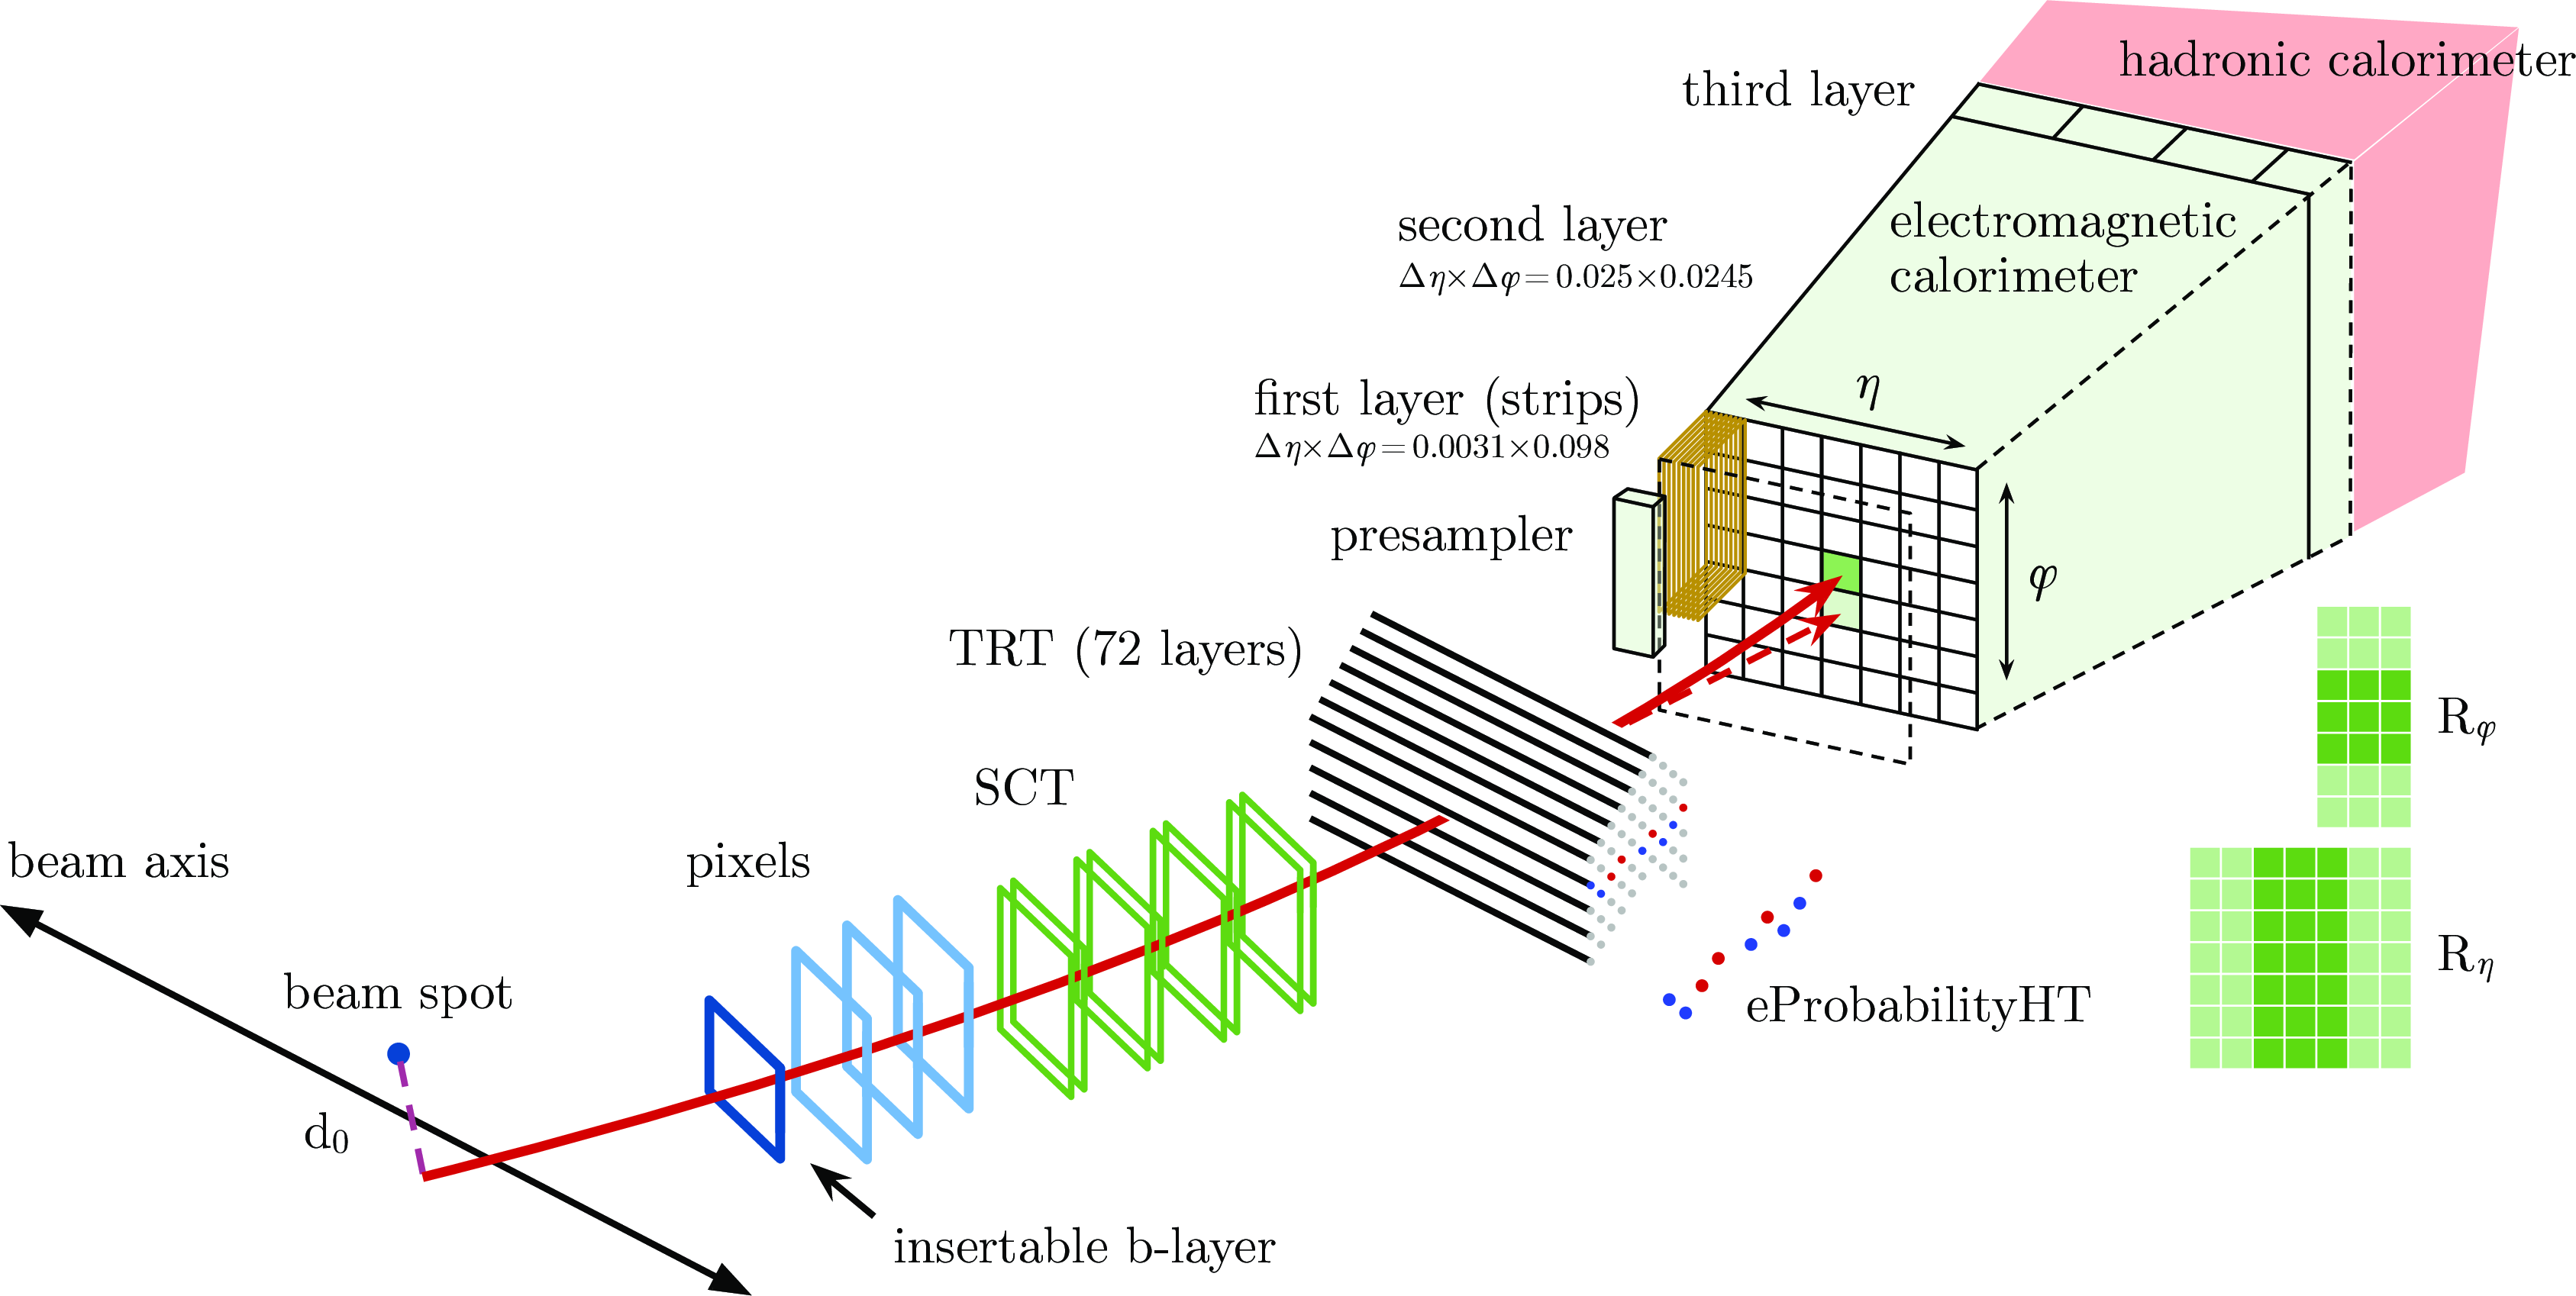
\includegraphics[width=1.2\textwidth]{figs/egamma/electron_variables.png}}
  \caption[Depiction of an electron traversing the ATLAS detector.
          The TRT extends to $|\eta|<2.0$, and the SCT and pixel detectors out to $|\eta|<2.47$.]
          {Depiction of an electron traversing the ATLAS detector.
          The TRT extends to $|\eta|<2.0$, and the SCT and pixel detectors out to $|\eta|<2.47$.
          Electron discriminating variables are described in Sections~\ref{sec:egamma:calvars} to \ref{sec:egamma:trackcalvars}.}
  \label{fig:egamma:LHvariablegraphic}
\end{figure}
For use in the electron identification, the likelihood discriminant, effectively the test statistic in a modified likelihood ratio, is constructed by creating a set of probability distribution functions (pdfs) from a list of $n$ electron identification variables with power for discriminating signal from background.
From the product of these pdfs the likelihood, $\mathcal{L}_{S}$ ($\mathcal{L}_{B}$), for signal (background) can be formed as is seen in Equation~\ref{eq:likelihoods} below.
%A given electron has a set of variable values $x$ associated with it.
\begin{equation}
\mathcal{L}_{S(B)}(\bf{X})=\prod_{i=1}^{n} P_{S(B),i}(x_{i})
\label{eq:likelihoods}
\end{equation}
$P_{S,i}(x_{i})$ is the value of the signal pdf for quantity $i$ at value $x_i$ and
$P_{B,i}(x_{i})$ is the corresponding value of the background pdf.
The signal is prompt electrons, while the background is the combination of jets that mimic the signature of prompt electrons, electrons from photon conversions in the detector material, and non-prompt electrons from the decay of hadrons containing heavy flavors.
The quantities selected for the LH are mostly uncorrelated, and any residual correlations are neglected.
The electron is given a score, or discriminant (or test statistic) value $d_{\mathcal{L}}$, based on the following equation, which combines information from this entire variable set:
For each electron candidate, a discriminant $d_{L}$ is formed: 
\begin{equation}
  \label{eq:egamma:discriminant}
d_{\mathcal{L}} = \frac{\mathcal{L}_{S}}{\mathcal{L}_{S} + \mathcal{L}_{B}};
\end{equation}
The electron LH identification is based on this discriminant.
The discriminant $d_L$ nominally has a sharp peak at unity (zero) for signal (background); this sharp peak makes it inconvenient to select operating points as it would require extremely fine binning.
An inverse sigmoid function is used to transform the distribution of the discriminant of Equation~\ref{eq:egamma:discriminant}:
\begin{equation*}
  \label{eq:inverse_sigmoid_transformation}
  d^\prime_{\mathcal{L}} = -\tau^{-1}\ln(d_{\mathcal{L}}^{-1} - 1),
\end{equation*}
where the parameter $\tau$ is fixed to 15~\cite{Hocker}.
As a consequence, the range of values of the transformed discriminant no longer varies between zero and unity.
This transformation results in distribution will be positive and peak near unity for signal and will be negative and broad for background. 
Operating points are then defined by a chosen value of the transformed discriminant: electron candidates with values of $d^\prime_{L}$ larger than this value are considered signal.
An example of the distribution of a transformed discriminant is shown in Figure~\ref{fig:egamma:discriminant} for prompt electrons from $Z$-boson decays and for background.
This distribution illustrates the effective separation between signal and background encapsulated in this single quantity.
By scanning over this distribution and computing the signal efficiency and corresponding background rejection for each sampled discriminant value the ROC curve in Figure \ref{fig:egamma:ROC} can be generated.
Note that the most optimal values are in the top right corner of the curve.  
The power of this technique is derived from the choice of the discriminating variables, which make up three categories: those which describe the shape and magnitude of the electron's energy in the calorimeters, those which describe the trajectory of the electron through the tracking detectors, and those which describe the matching between the tracks and the calorimeter clusters.  
\begin{figure}[t]
\centering
    \begin{subfigure}[b]{0.49\textwidth}
      \centering
      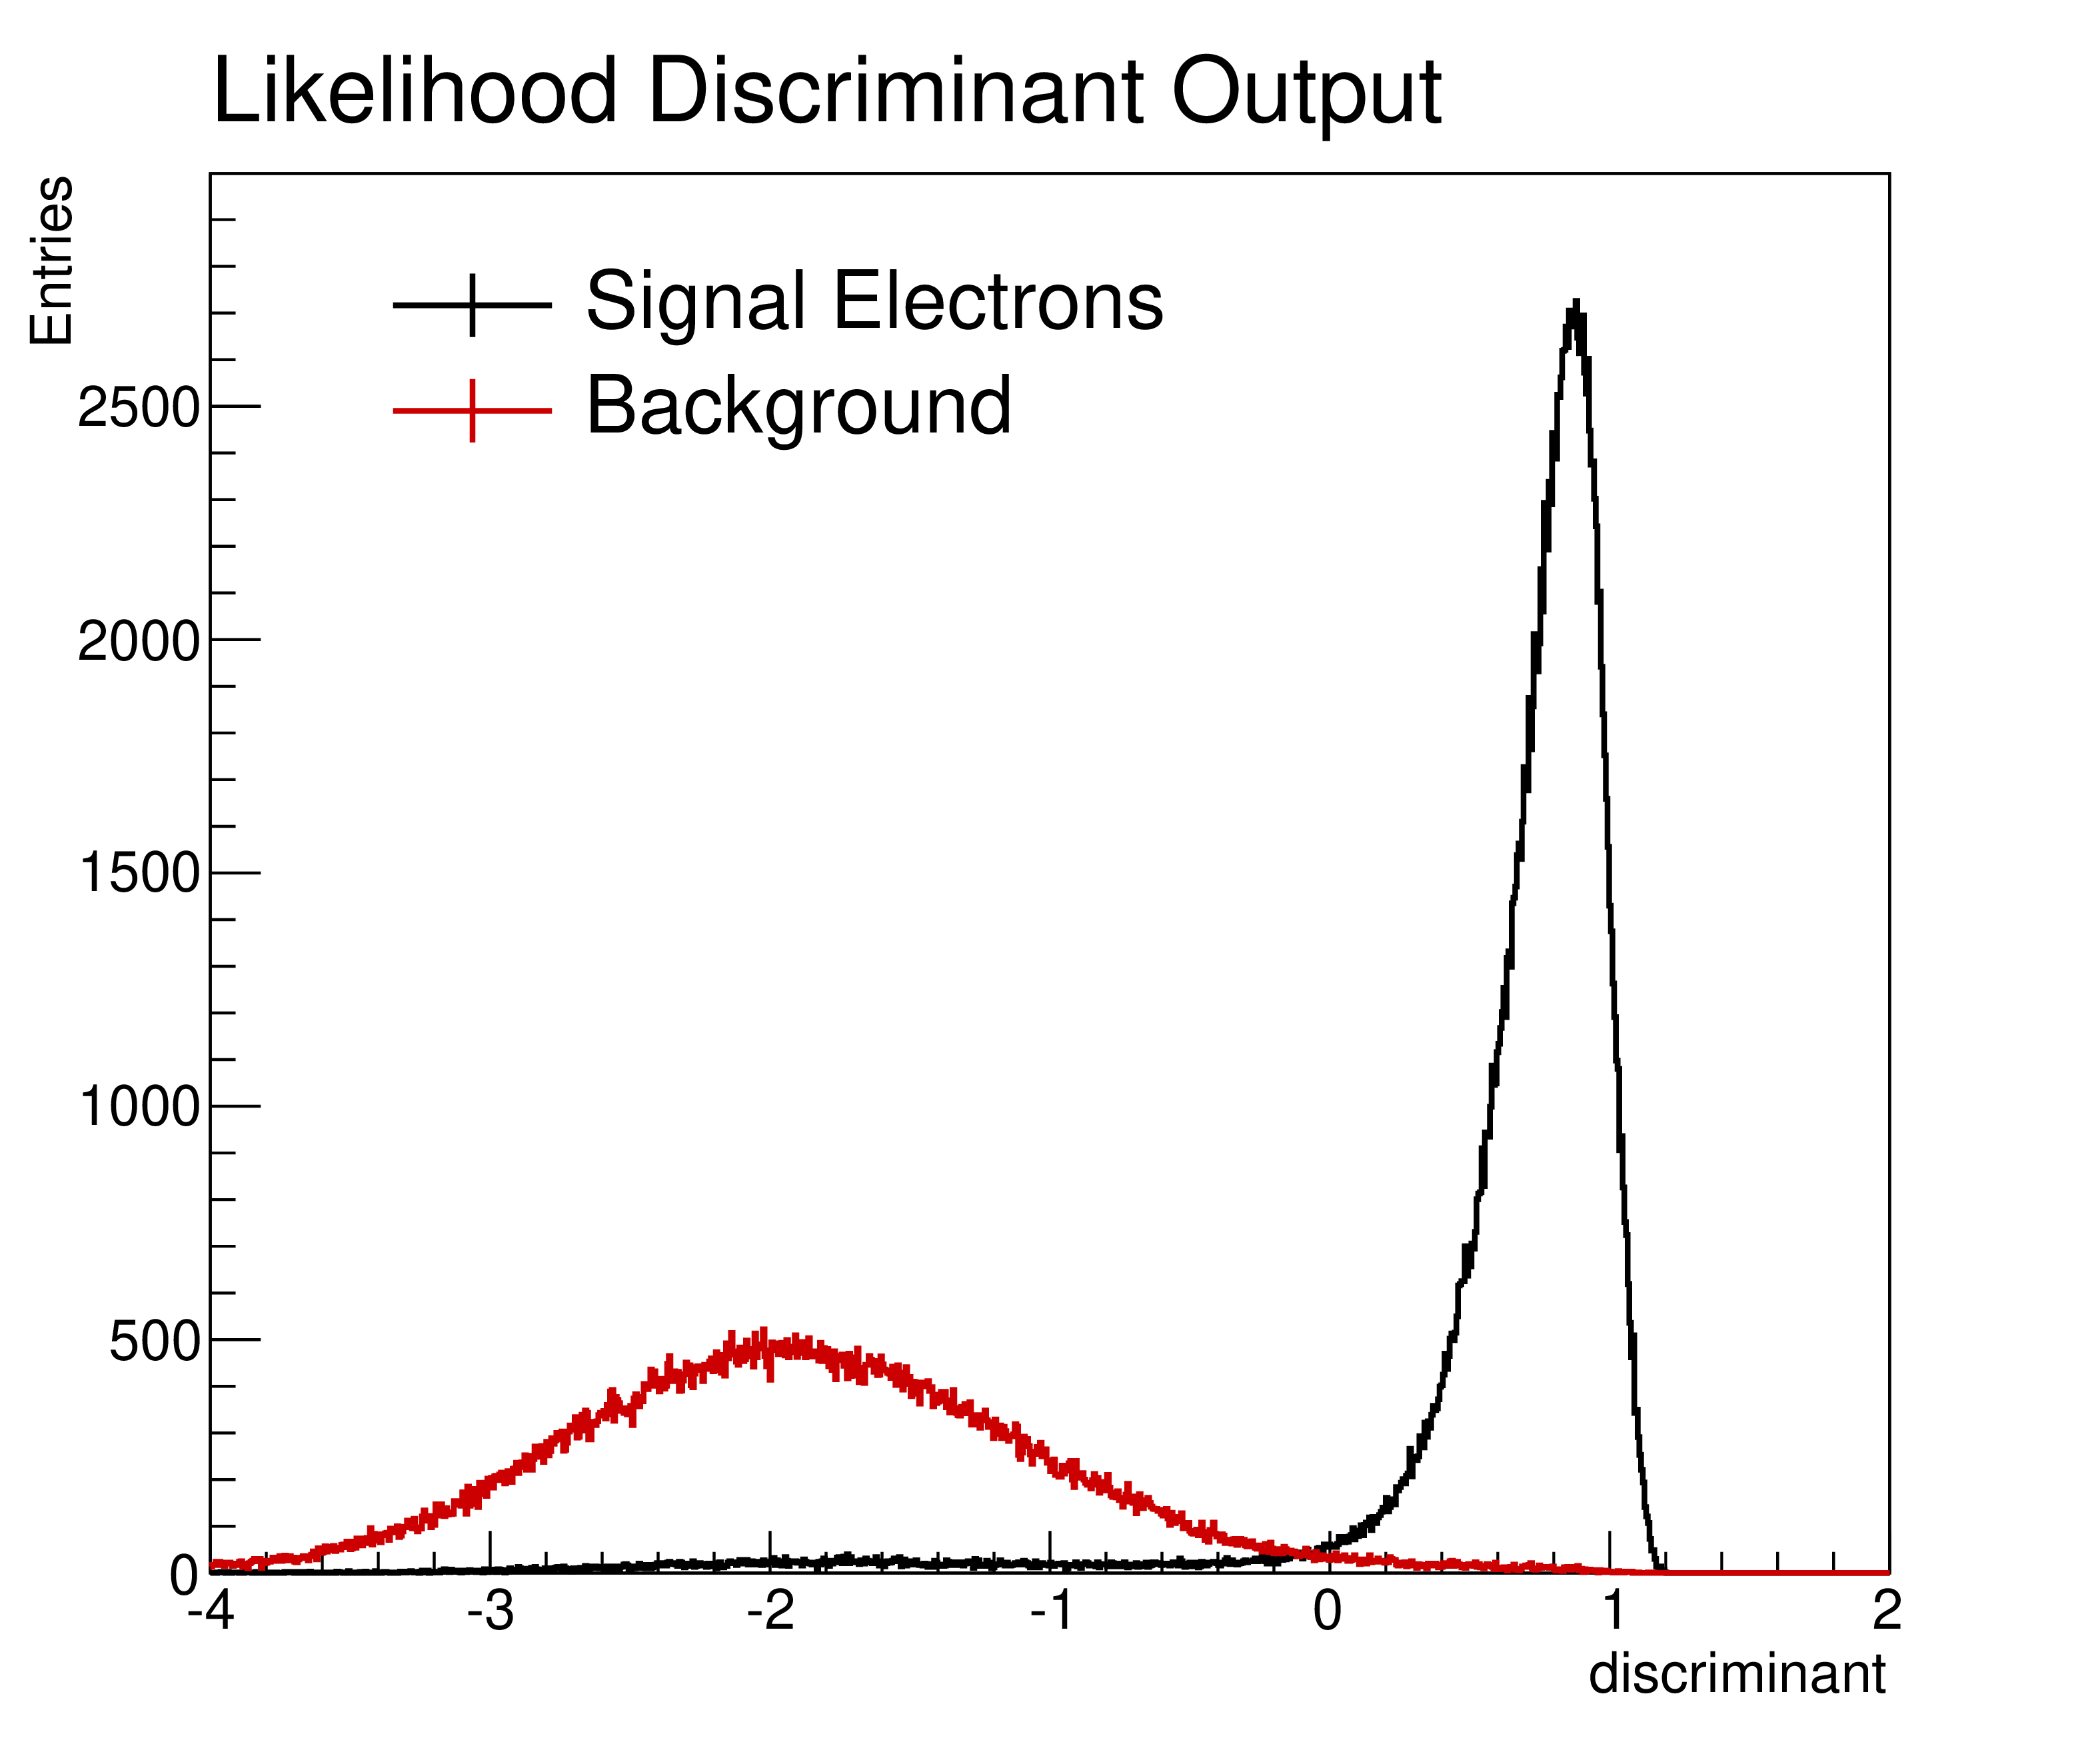
\includegraphics[width=1.0\textwidth]{figs/egamma/example_lh_output.png}
      \caption{}
      \label{fig:egamma:discriminant}
    \end{subfigure}
    \hfill
    \begin{subfigure}[b]{0.49\textwidth}
      \centering
      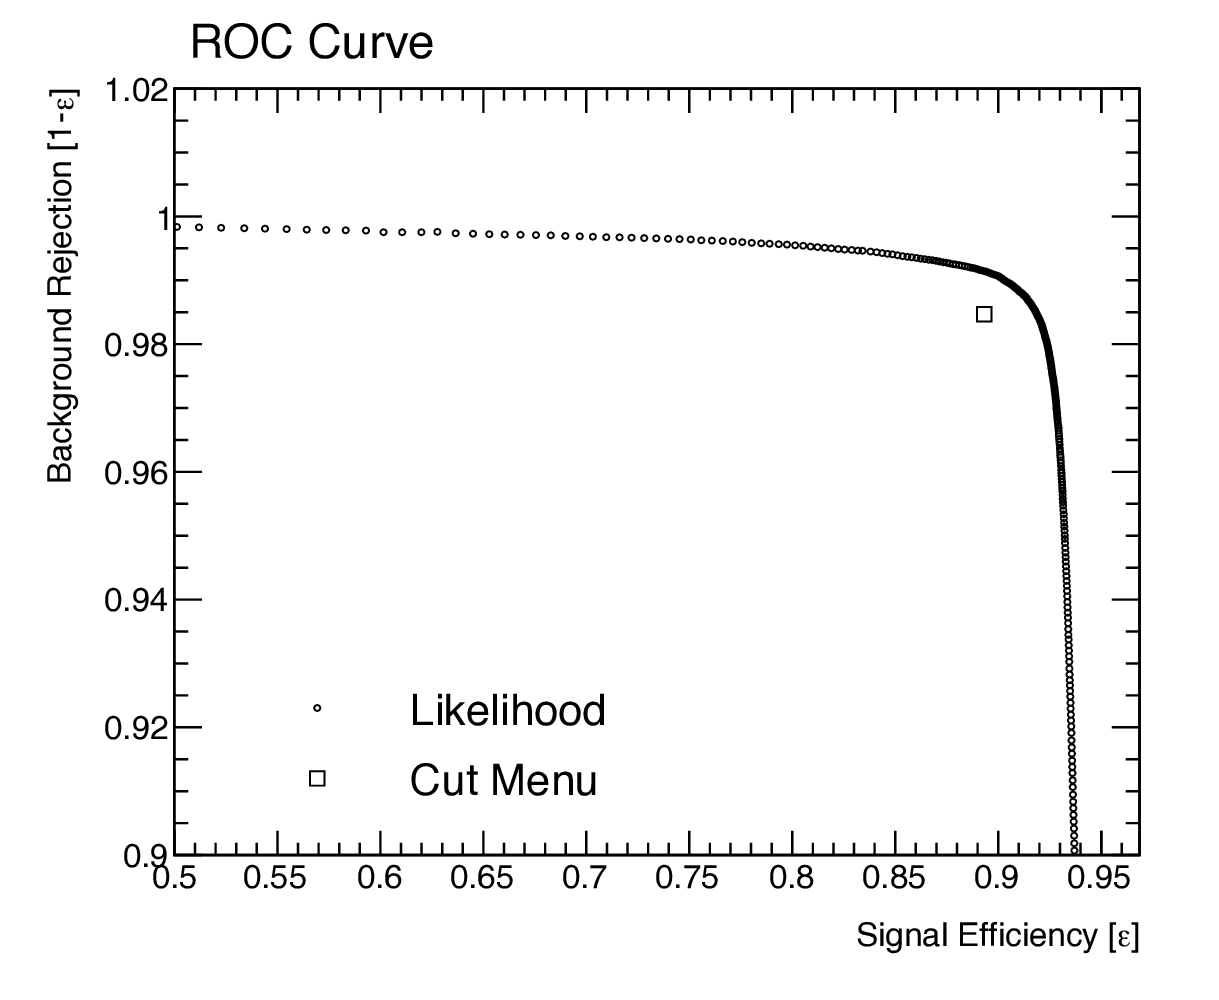
\includegraphics[width=1.0\textwidth]{figs/egamma/ROC.png}
      \caption{}
      \label{fig:egamma:ROC}
    \end{subfigure}
     \caption[]{
       The transformed LH-based identification discriminant $d^\prime_L$ for reconstructed electron candidates with good quality tracks with
    %%%  $30 < \Et < 35$~\GeV and $0.60 <|\eta|<0.8$.
       30~\GeV\ $<$ \Et\ $<$ 35~\GeV\ and \hbox{$|\eta|<0.6$}.
       The black histogram is for prompt electrons in a \Zee simulation sample, and the red (dashed-line) histogram is for backgrounds in a generic two-to-two process simulation sample.
       The histograms are normalised to unit area.
  }
\label{fig:egamma:discriminantROC}
\end{figure}

\subsection{LH Calorimeter Variables}
\label{sec:egamma:calvars}
Here the LH discriminating variables which characterize the shape and depth of the EM showers deposited in the EM and hadronic calorimters by an electron are described. 
%There are nine calorimeter variables that contribute to the LH.
The variable \rhadone\ is the ratio of \et\ in the first layer of the hadronic calorimeter to the \et ~in the EM calorimeter and is a measure of the energy leakage to the EM shower from the EM calorimeter to the hadronic calorimeter.
\rhadone\ is used to distinguish electrons and hadrons based on their shower depth.
For isolated electrons, the shower is expected to be well-contained within the EM calorimeter and \rhadone\ is expected to be centered very sharply around zero, while for background a long positive tail is expected.
This distribution can be see in Figure~\ref{fig:egamma:calorimeterDepth_pdfs}.
Other depth ratio variables inside the EM calorimeter, \fI\ and \fIII, seek to characterize the evolution of the shower as it traverses the EM calorimeter.
\fIII, is the ratio of the total energy in the EM calorimeter to the energy in the third layer. 
This variable encapsulates the expectation that an electron will deposit most of its energy in the first two layers of the EM calorimeter.
As shown in the \fIII\ distribution in Figure \ref{fig:egamma:calorimeterDepth_pdfs} the signal peaks close to zero and has a broader width than \rhadone.
The variable \fI\ is the ratio of the energy in the first layer of the EM calorimeter to the total energy in the calorimeter for the EM cluster of interest.
While this variable is not expected to sharply peak at any specific value, features picked up by \fI\ when used in conjunction with the entire suite of discriminating variables in the LH make it a powerful component.  
Its distribution for both signal and background is shown in Figure~\ref{fig:egamma:calorimeterDepth_pdfs}.
%The next set of variables target the second layer of the EM calorimeter.
The energy width variables \weta, \rphi, and \reta\ distinguish narrow electron showers from diffuse hadronic showers.
The variable \weta\ is designed to measure the lateral shower width of the object, defined as \begin{equation*}
    w_{\eta 2} = \sqrt{(\Sigma E_i \eta_i^2)/(\Sigma E_i) -((\Sigma E_i\eta_i)/(\Sigma E_i))^2}
\end{equation*}
The \weta\ distribution for both signal and background is shown in Figure~\ref{fig:egamma:calorimeterWidth_pdfs}.
The variable \Rphi, the ratio of the energy of 3$\times$3 cells over the energy in 3$\times$7 cells centered at the electron cluster position handles the expectation that the cluster should have a narrow width in the $\phi$ direction.
While \reta, the ratio of the energy of 3$\times$7 cells over the energy in 7$\times$7 cells centered at the electron cluster position, handles the expectation that the cluster should also have a narrow width in the $\eta$ direction.
Finally, \deltaEmax, the difference between the two largest maxima (if two maxima exist) in the finely segmented strips layer of the cluster, divided
by the sum of the two maxima, is calculated to check for multiple incident particles.
All of these variables are summarized in Table \ref{tab:IDcuts}.

\subsection{LH Tracking Variables}
\label{sec:egamma:trackvars}
These are the variables that are associated with the tracking detectors and the track fit.
The variable \trackdO, the transverse impact parameter and \dOSignificance, the significance of the transverse impact parameter defined as the ratio of \trackdO\ to its uncertainty, help to distinguish electrons prompt electrons from those from the semileptonic decay of long-lived heavy flavor hadrons.
The \deltapoverp\ variable is associated with the GSF track fit characterizes the track's energy loss due to bremsstrahlung and can help discriminate electrons from charged hadrons that do not lose as much energy in the ID.
The TRT provides discrimination between electrons and heavier objects based on the principle of transition radiation.
Charged particles with larger $\gamma$-factors (light particles, electrons being the lightest charged particle) radiate more photons than those with lower $\gamma$-factors (more massive particles like muons, charged pions, protons) when traversing the radiator foil inside the TRT.
Those photons in turn induce high-threshold hits in the detector.
In Run-1, only the ratio of high-threshold hits to the total number of TRT hits along the reconstructed track, (\TR), was used from the TRT as a signature of transition radiation to distinguish electrons from hadrons.
However, beginning in 2012, leaks in the TRT gas system resulted in large losses of expensive xenon gas.
To cope with this problem, the gas in some TRT modules was switched from xenon to argon, which is less expensive, beginning in the 2015 data taking period. 
More and more modules have been switched since.
Figure~\ref{fig:egamma:TRTGas} shows the gas configuration for both 2015, 2016, 2017, and 2018 data taking years for both the barrel and endcap layers.
%Can't find analogous figure for 2017
The use of argon gas leads to less transition radiation being produced and therefore a lower probability for a high-threshold hit as compared to xenon.
To compensate for the subsequent loss of performance, a tool was developed to calculate a likelihood ratio between electrons and backgrounds based on the high threshold hit information.
The TRT likelihood method uses the high-threshold probability of each TRT hit to construct a discriminant variable, referred to here as \TRTPID.
The probability for each TRT hit to exceed the high level threshold depends on the straw gas type, the Lorentz factor $\gamma$ calculated from the track \pt\ under a particle type hypothesis, the TRT occupancy local to the track, and the geometry: detector partition, straw layer, track-to-wire distance and the hit coordinates (z for the barrel and radius for the endcaps).
The ratio of probabilities between the electron hypothesis and pion hypothesis is then this discriminating variable \TRTPID.
%The high threshold probability of each hit is determined as a function of the location of the straw in the detector and the track-to-wire distance of the hit; the probability is calculated separately for electron and pion hypotheses. 
These variables are summarized in Table \ref{tab:IDcuts}.


\subsection{LH Track-Cluster Matching Variables}
\label{sec:egamma:trackcalvars}
Variables that describe the quality of the match between the track and the cluster can be used to distinguish electrons from primarily converted photons or charged hadrons.
The variable \deltaeta, is the $\Delta\eta$ between the cluster position in the first layer and the extrapolated track.
The variable \deltaphires, is the $\Delta\phi$ between the cluster position in the second layer of the EM calorimeter and the momentum-rescaled track, extrapolated from the perigee, times the charge $q$.
These variables are summarized in Table \ref{tab:IDcuts}.

\subsection{Non-LH Variables}
\label{sec:egamma:nonLHvars}
In addition to the LH decision which is a function of the multivariate product of the pdfs associated with the variables just described in previous Sections \ref{sec:egamma:calvars} to  \ref{sec:egamma:trackcalvars}, there are several variables that are used directly as a selection criterion that the electron object must satisfy as well.
The track quality criteria variables $n_{\mathrm{Blayer}}$, $n_{\mathrm{Pixel}}$, and $n_{\mathrm{Si}}$ refer to a required number of track hits in the B-layer, Pixel detector, and Silicon Strips detector respectively. 
The next two variables were implemented to address inefficiencies of the LH at high \pt ~for the \Tight\ operating point.
%discussed in more detail in Section \ref{somehighptsection}.
These additional variables are \eoverp\ and \wstot, which are not included in the LH as pdfs due to their correlations with the other variables which are used, as well as concerns regarding their modeling in the MC (e.g. the resolution of \eoverp\ can degrade at high \pt, but this may not be properly represented in the MC, which would make it a sub-optimal variable to use as a pdf in the LH). 
These variables are summarized in Table \ref{tab:IDcuts} and appear in the table with a ``C'' in the ``Usage'' column.

\begin{table*}
%\caption{Definitions of electron discriminating variables, the types of backgrounds the variables help to discriminate against, and if a variable is used as a likelihood pdf ($\mathcal{L}$) or used as a rectangular cut (C). The $^{*}$ refers to the fact that the $E/p$ and \wstot variables are
%  only used for electrons with $\pt > 150~\GeV$ for the \Tight identification operating point (in software release 20.7), and are not used for the looser operating points.}
\caption[Type and description of the quantities used in the electron identification.]{Type and description of the quantities used in the electron identification.
The columns labelled ``Rejects'' indicate whether a quantity has significant discrimination power between prompt electrons and light-flavor (LF) jets, photon conversions ($\gamma$), or non-prompt electrons from the semileptonic decay of hadrons containing heavy-flavor (HF) quarks ($b$- or $c$-quarks).
In the column labelled ``Usage,'' an ``LH'' indicates that the pdf of this quantity is used in forming $\mathcal{L}_{S}$ and $\mathcal{L}_{B}$ (defined in Equation~\ref{eq:likelihoods}) and a ``C'' indicates that this quantity is used directly as a selection criterion. 
In the description of the quantities formed using the second layer of the calorimeter, 3$\times$3, 3$\times$5, 3$\times$7, and 7$\times$7 refer to areas of $\Delta\eta \times \Delta\phi$ space in units of $0.025 \times 0.025$.
}
\label{tab:IDcuts}
\scriptsize
\renewcommand{\arraystretch}{1.30}
\begin{center}
\begin{tabular}{|l|l|l|c|c|c|c|}
\hline
Type & Description & Name &  \multicolumn{3}{c|}{Rejects} & Usage  \\
 & & & LF & $\gamma$ & HF &\\
\hline
 Hadronic & Ratio of \et\ in the first layer of the hadronic calorimeter  & \rhadone & x & x &  & LH \\ 
 leakage & to \et\ of the EM cluster & & & & & \\
& (used over the range $|\eta| < 0.8$ or $|\eta| > 1.37$)  & & & & & \\
\cline{2-7}
  & Ratio of \et\ in the hadronic calorimeter &  & & & & \\
  &  to \et\ of the EM cluster & \rhad & x & x &  & LH  \\
 & (used over the range $0.8 <|\eta| < 1.37$) & & & & & \\
\hline
Third layer & Ratio of the energy in the third layer to the total energy & & & & &\\
of the EM   & in the EM calorimeter. This variable is only used for & & & & & \\
calorimeter & \et\ $< 80$~\GeV, due to inefficiencies at high \et, and is& \fIII & x & & & LH \\
                & also removed from the LH for $|\eta| > 2.37$, where it is& & & & & \\
                & poorly modelled by the simulation. & & & & & \\
\hline
Second layer & Lateral shower width, $\sqrt{(\Sigma E_{i} \eta_{i}^{2})/(\Sigma E_{i}) -((\Sigma E_{i}\eta_{i})/(\Sigma E_{i}))^{2}}$, & & & & & \\
of the EM & where $E_i$ is the energy and $\eta_{i}$ is the pseudorapidity of cell $i$  & \weta & x & x & & LH \\
calorimeter. & and the sum is calculated within a window of 3$\times$5 cells & & & & & \\
\cline{2-7}
& Ratio of the energy in 3$\times$3 cells over the energy in 3$\times$7 cells & \rphi & x & x &  & LH  \\
& centered at the electron cluster position & & & & & \\
\cline{2-7}
& Ratio of the energy in 3$\times$7 cells over the energy in 7$\times$7 cells  & \reta & x & x & x & LH  \\
& centered at the electron cluster position & & & & & \\
\hline
First layer & Shower width, $\sqrt{(\Sigma E_i (i-i_{\mathrm{max}})^{2})/(\Sigma E_{i})}$, where $i$ runs &   & & & & \\  
of the EM & over all strips in a window of $\Delta\eta \times \Delta\phi \approx 0.0625 \times 0.2$,   & \wstot & x & x & x & C \\
calorimeter & corresponding typically to 20 strips in $\eta$, and $i_{\mathrm{max}}$ is the & & & & &                  \\
		        & index of the highest-energy strip, used for \et\ $>$ 150~\gev\ only        &  & & & &   \\
\cline{2-7}
                     & Ratio of the energy difference between the maximum &    & & & &  \\
                     & energy deposit and the energy deposit in a secondary & \deltaEmax & x & x & & LH  \\
                     & maximum in the cluster to the sum of these energies & & & & &   \\
\cline{2-7}     
& Ratio of the energy in the first layer to the total energy  & \fI & x & & & LH  \\
& in the EM calorimeter &  & & & & \\
\hline
Track & Number of hits in the innermost pixel layer &   $n_{\mathrm{Blayer}}$ & & x & & C \\
%conditions & &   $ $  & & & & \\
%discriminates against photon conversions &   $ $  & & & & \\
\cline{2-7}
conditions & Number of hits in the pixel detector        &    $n_{\mathrm{Pixel}}$ & & x & & C \\
\cline{2-7}
                     & Total number of hits in the pixel and SCT detectors  &   $n_{\mathrm{Si}}$  & & x & & C \\
\cline{2-7}
                     & Transverse impact parameter relative to the beam-line
		     % cut-based: trackd0_physics:Transverse impact parameter with respect to the beam spot,
		     % LH: el_trackd0pvunbiased and el_tracksigd0pvunbiased
		                                                  &       \trackdO  & & x & x & LH \\
\cline{2-7}
                     & Significance of transverse impact parameter &       \dOSignificance  & & x & x & LH  \\
                     & defined as the ratio of \trackdO to its uncertainty                     &  & & & &              \\
\cline{2-7}
                     & Momentum lost by the track between the perigee &   \deltapoverp & x & & & LH \\
                     & and the last measurement point divided by the   & & & & & \\
                     & momentum at perigee & & & & & \\
\hline
%TRT                 & Total number of hits in the TRT      & $n_\mathrm{TRT}$          \\
%\cline{2-3}
%TRT                 & Ratio of the number of high-threshold hits to the total number of  hits in the TRT &    \TRTHighTHitsRatio  \\
%\cline{2-3}
TRT & Likelihood probability based on transition radiation &   \TRTPID & x & & & LH  \\
                          & in the TRT & & & & & \\
\hline
Track-- & $\Delta\eta$ between the cluster position in the first layer &   \deltaeta & x & x & & LH  \\
cluster &  and the extrapolated track & & & & &   \\
%\cline{2-3}
%  matching    & $\Delta\phi$ between the cluster position in the middle layer and the extrapolated & \deltaphires\\
%&   track, where the track momentum is rescaled to the cluster energy &  \\
%&   before extrapolating the track to the middle layer of the calorimeter  &  \\
%\cline{2-7}
%     & $\Delta\phi$ between the cluster position in the middle layer and & \deltaphi & x & x & & $\mathcal{LH}$  \\
%  & $ $and the track extrapolated from the perigee & & & & & \\
%\cline{2-7}
%&   Defined as  \deltaphi, but the track momentum is rescaled &   & & & &  \\
%&   to the cluster energy before extrapolating the track from  & \deltaphires & x & x & & $\mathcal{LH}$  \\
%&   the perigee to the middle layer of the calorimeter  & & & & &  \\
\cline{2-7}
matching &   $\Delta\phi$ between the cluster position in the second layer &   & & & &  \\
&   of the EM calorimeter and the momentum-rescaled  & \deltaphires & x & x & & LH  \\
&   track, extrapolated from the perigee, times the charge $q$  & & & & &  \\
\cline{2-7}
                    & Ratio of the cluster energy to the track momentum, &       $E/p$   & x & x & & C\\
                    & used for \et $>$ 150~\gev\ only & & & & &  \\
%\hline
%Conversions         & Veto electron candidates matched to reconstructed photon  conversions            &  isConv \\
\hline
\end{tabular}
\end{center}
\end{table*}

\begin{figure}[h]
\centering
  \begin{subfigure}[b]{0.495\textwidth}
    \centering
    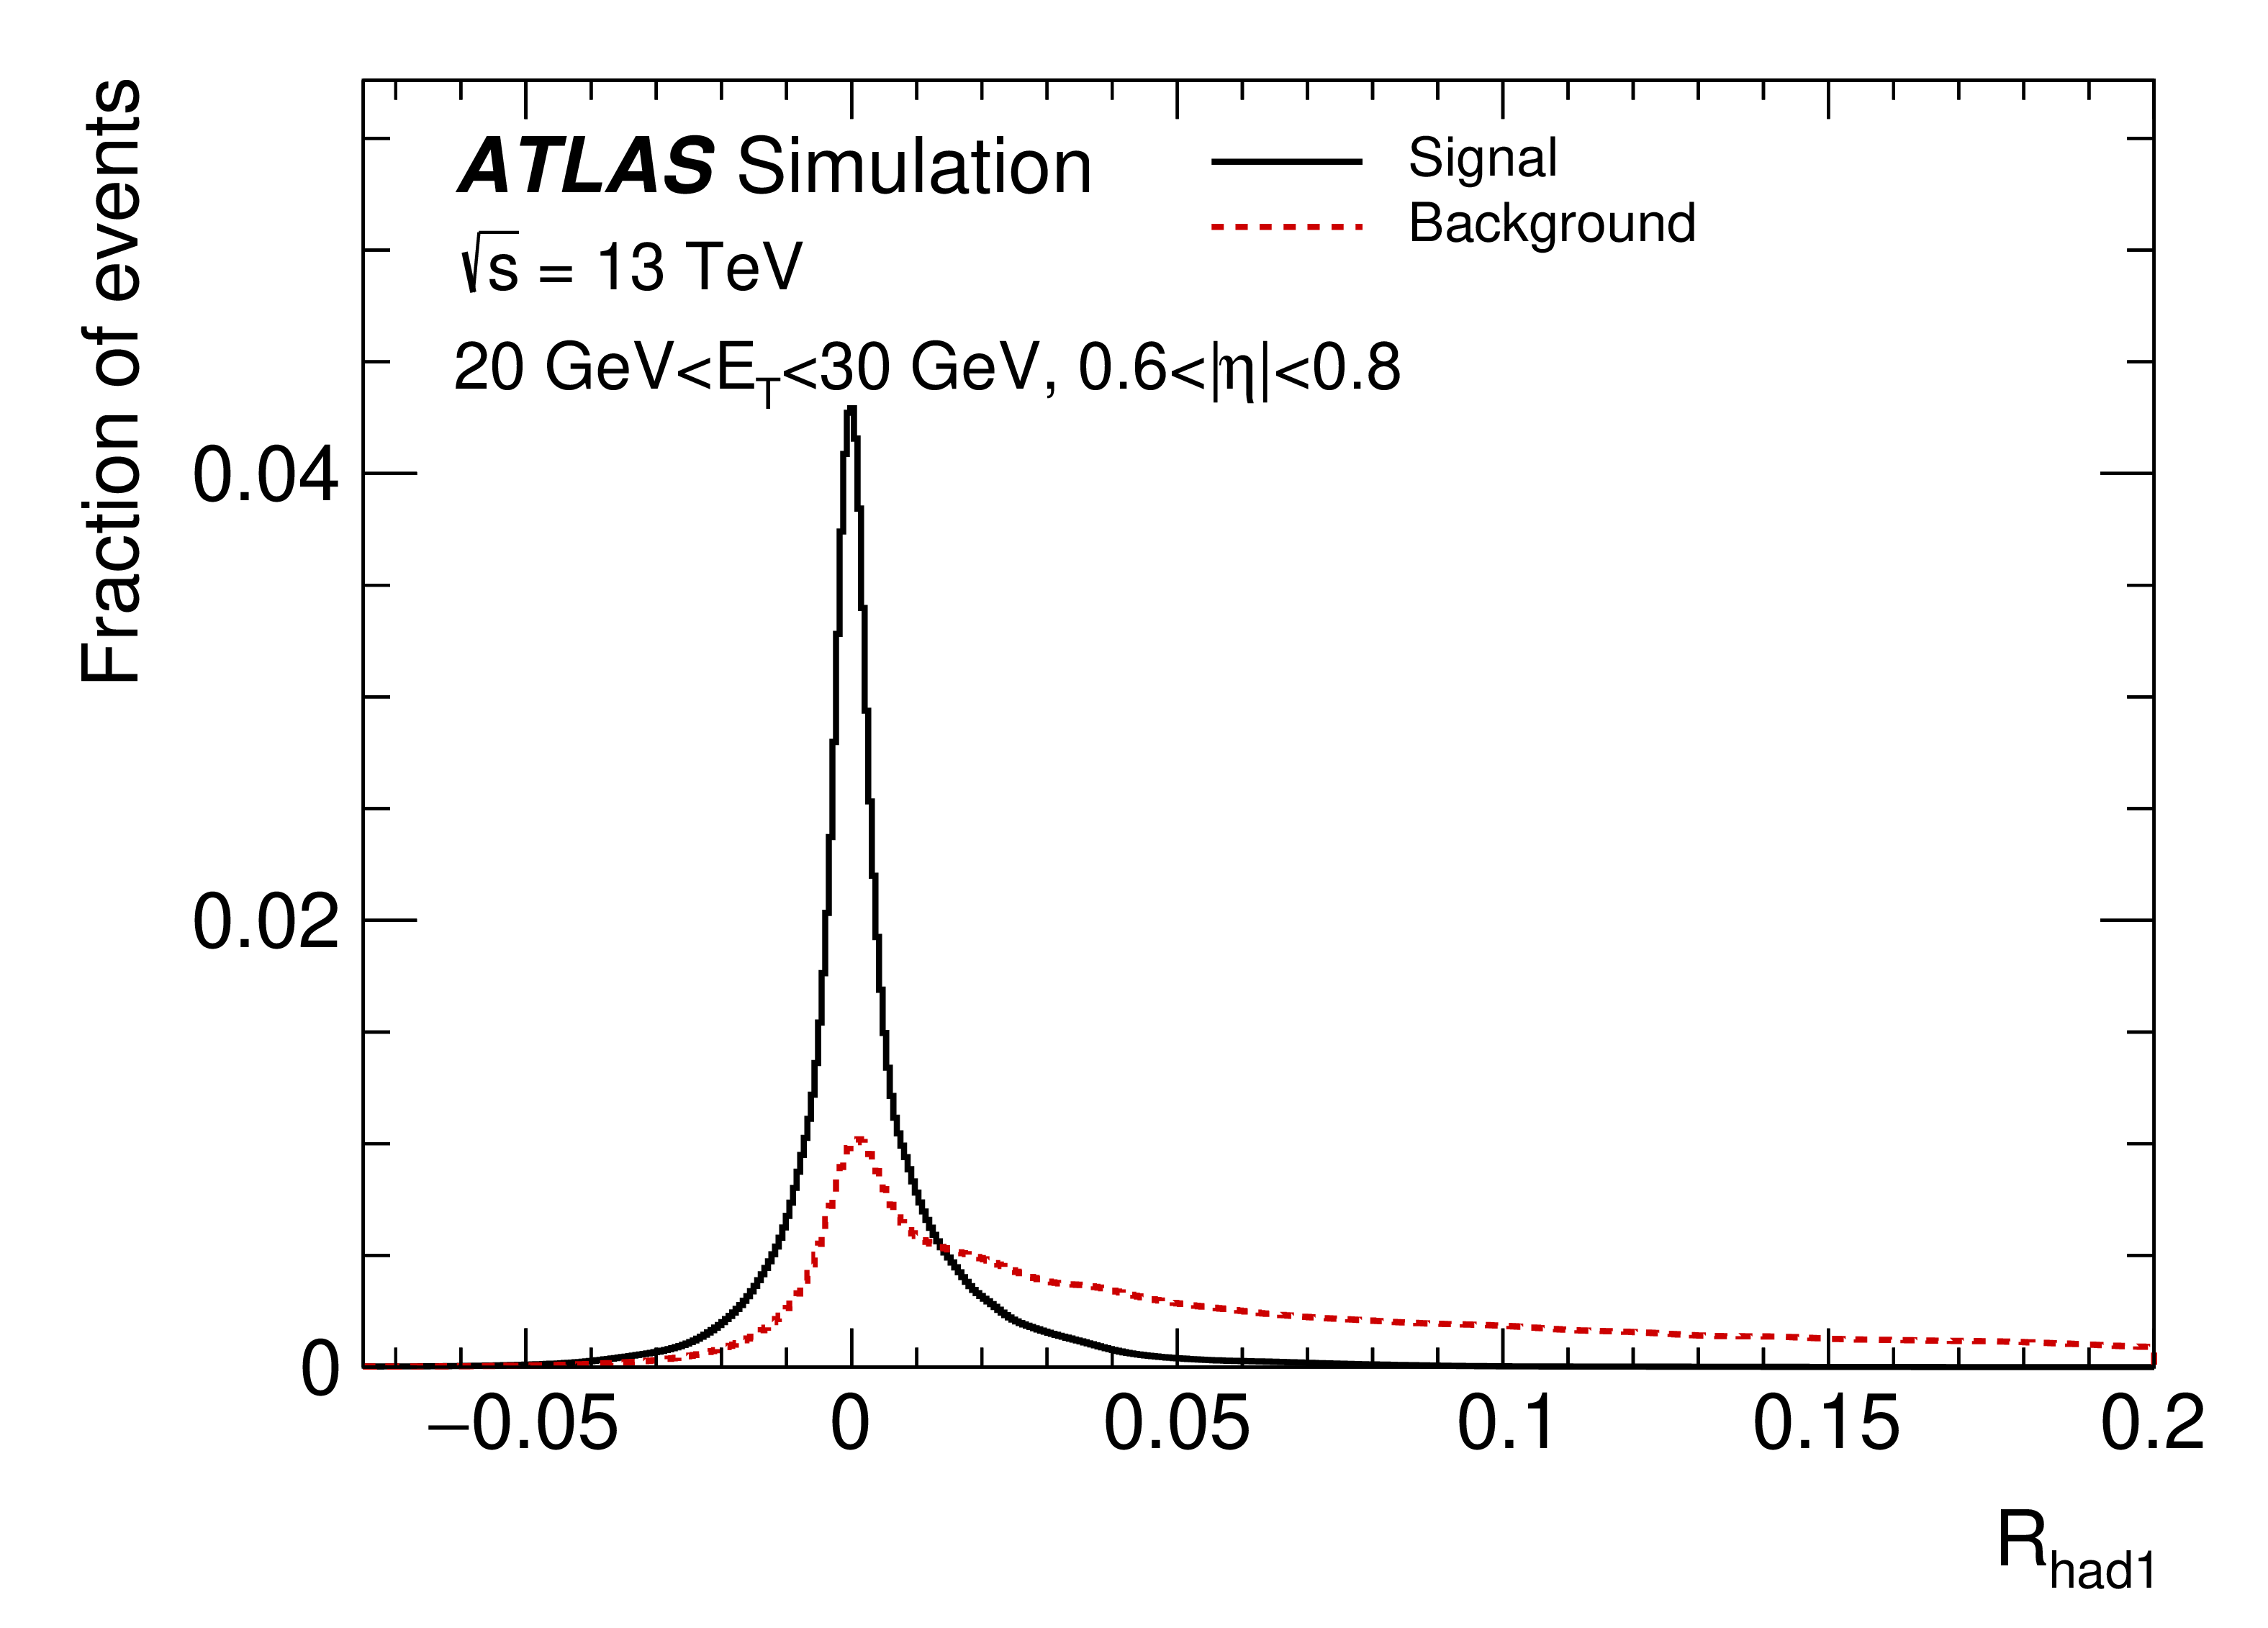
\includegraphics[width=1.0\textwidth]{figs/egamma/R_had1.png} 
    \label{fig:egamma:Rhad1}
  \end{subfigure}
  \hfill
  \begin{subfigure}[b]{0.495\textwidth}
    \centering
    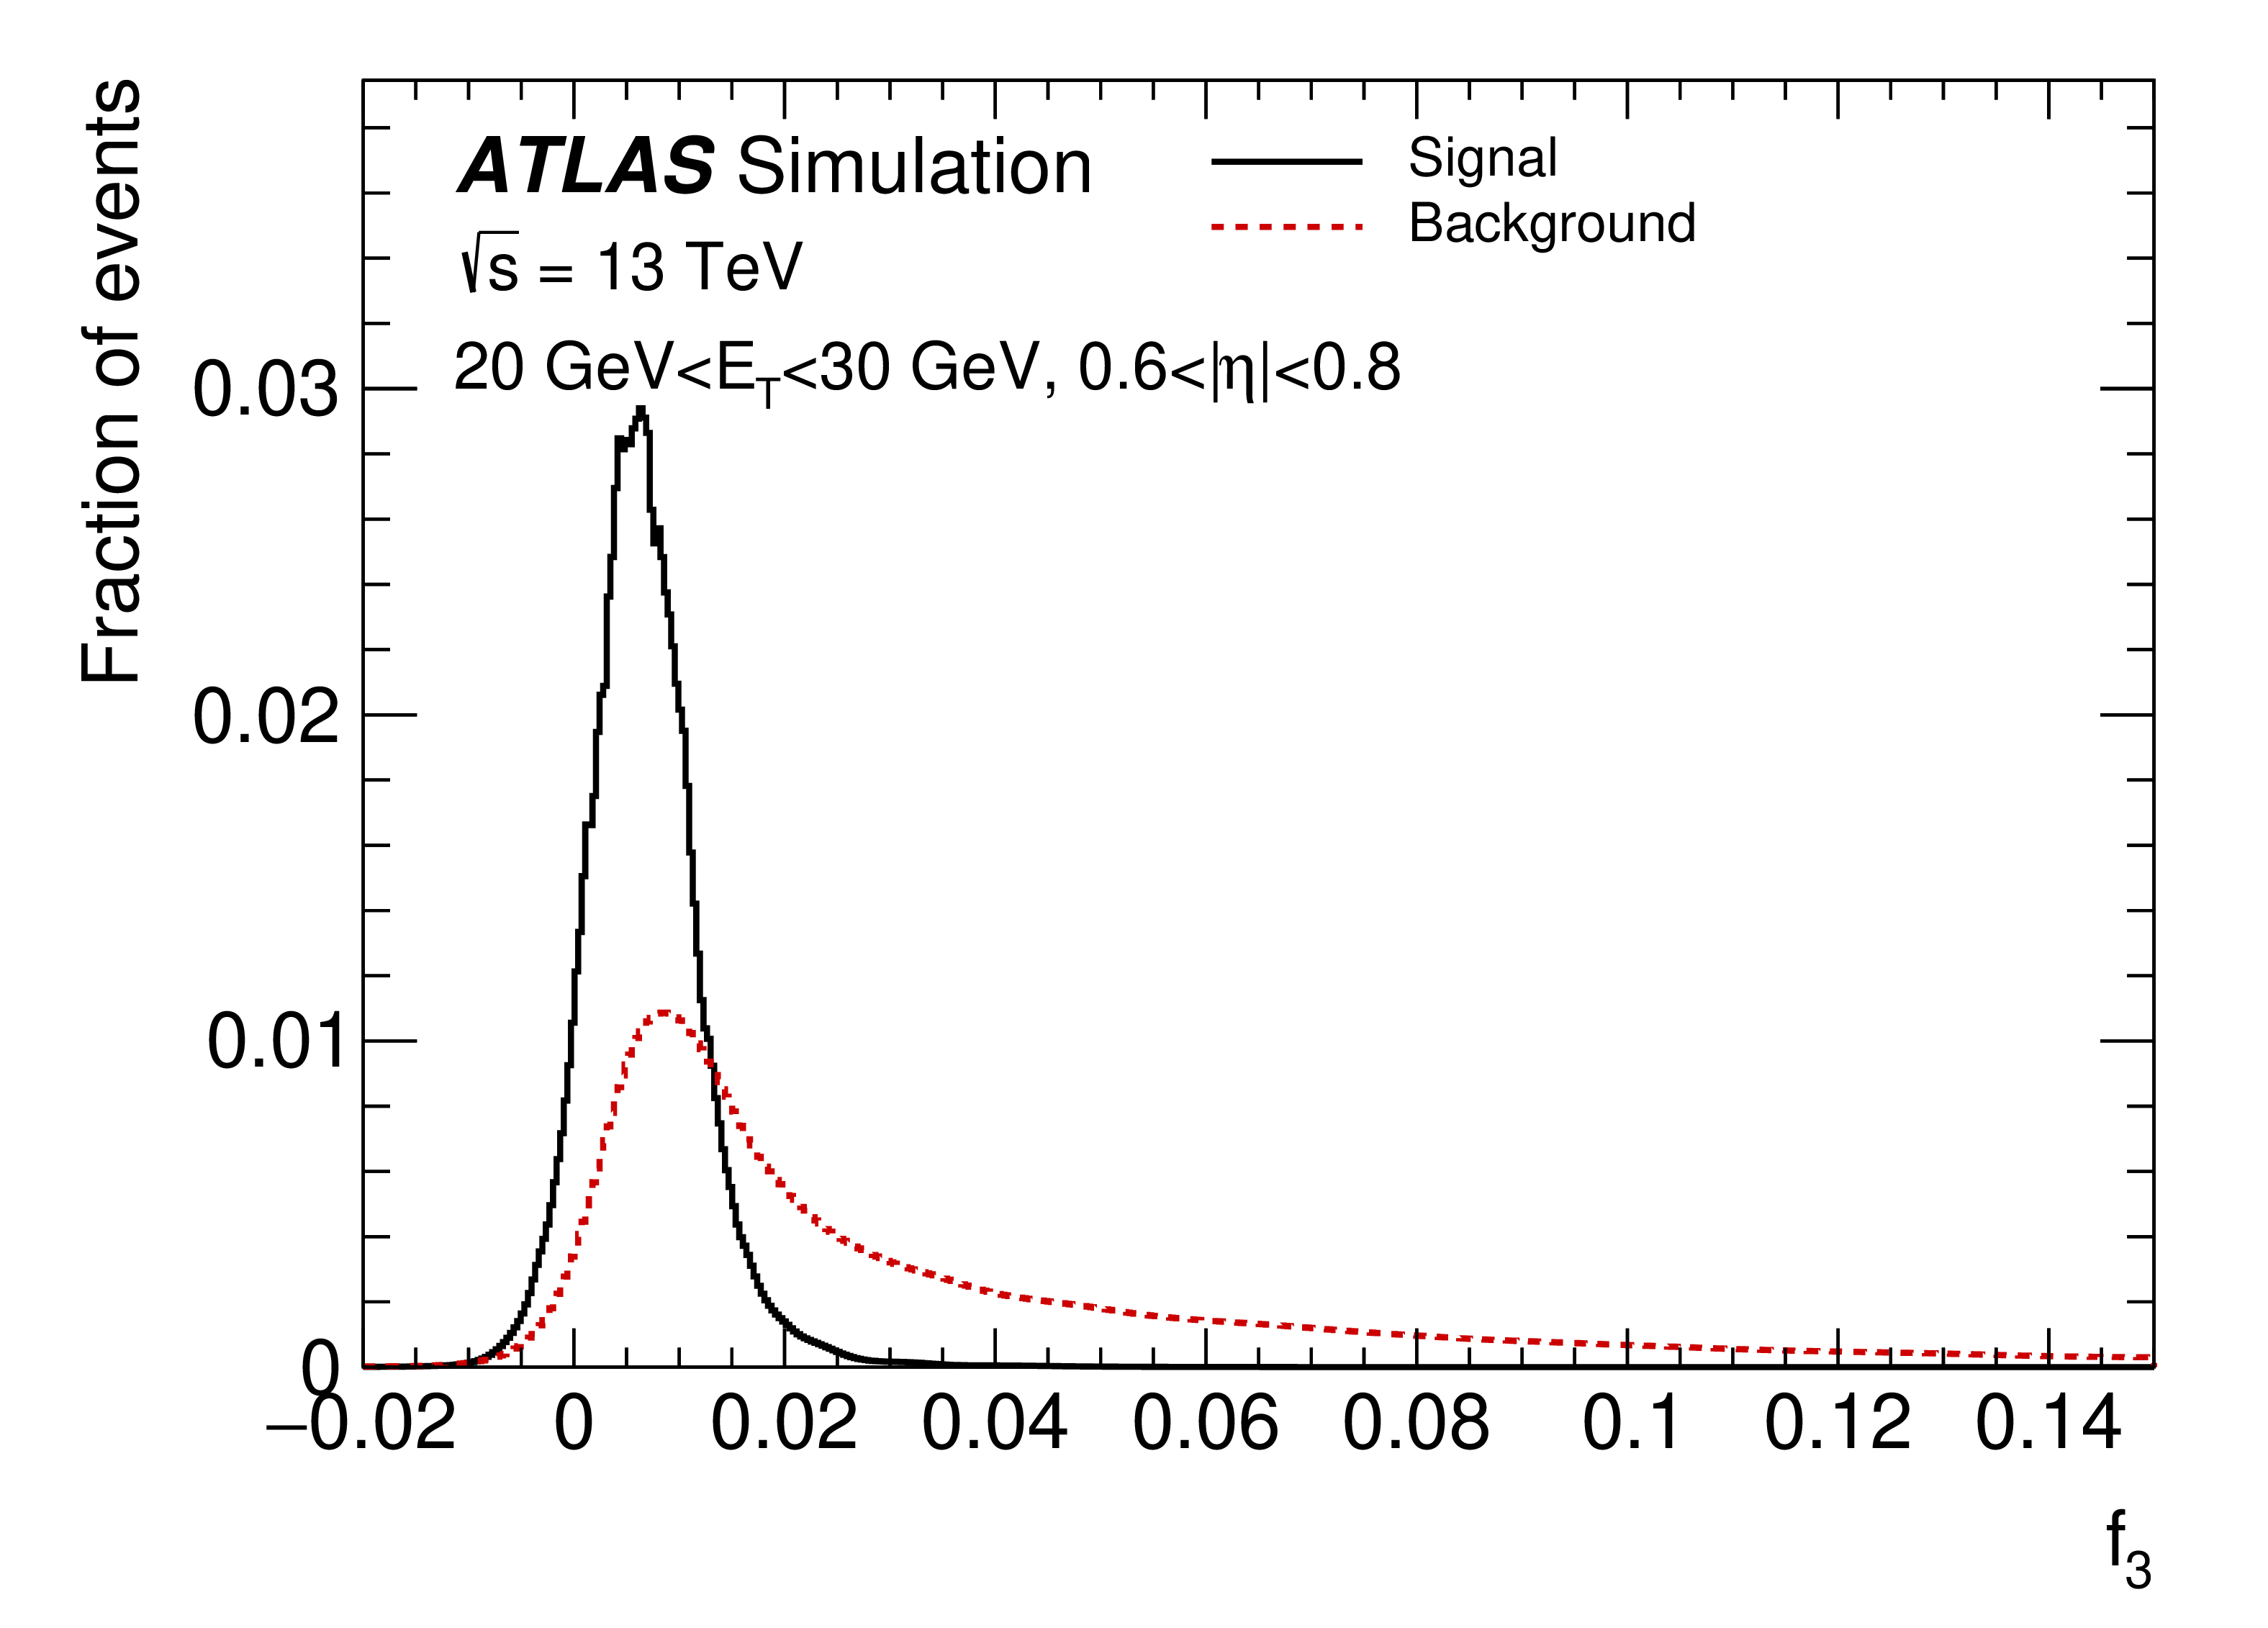
\includegraphics[width=1.0\textwidth]{figs/egamma/f3.png} 
    \label{fig:egamma:f3}
  \end{subfigure}
  \hfill
  \begin{subfigure}[b]{0.495\textwidth}
    \centering
    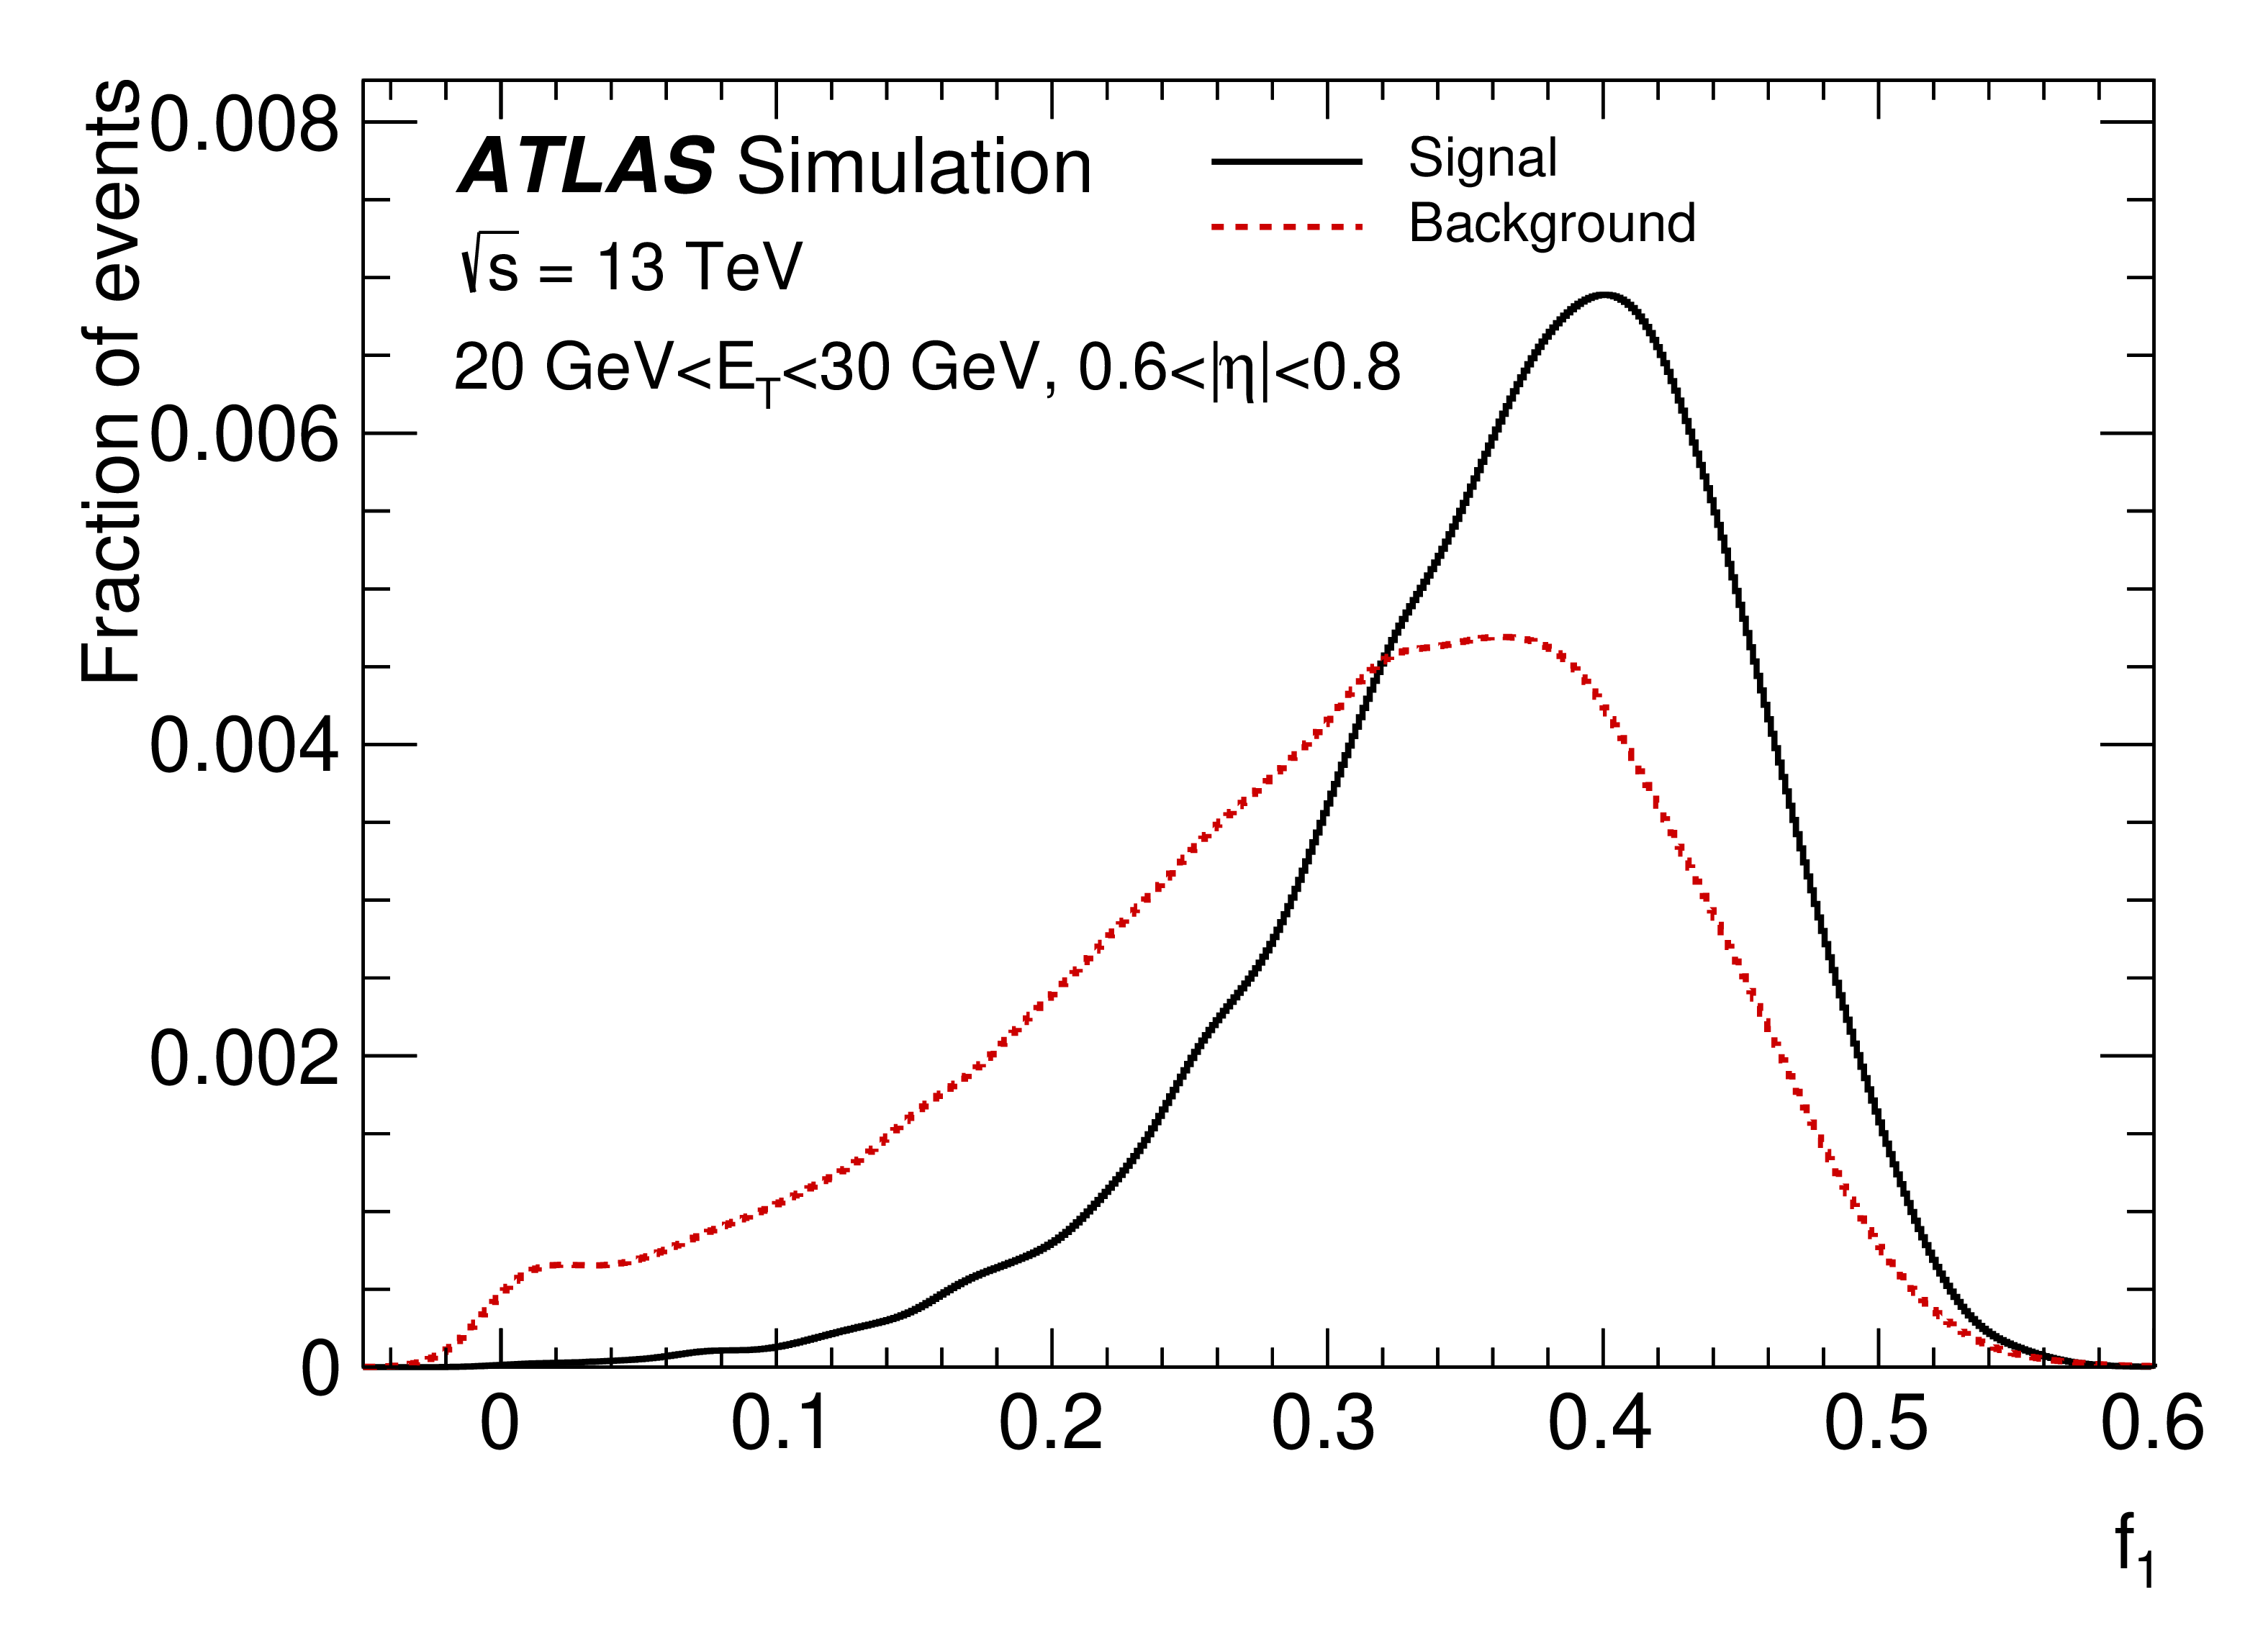
\includegraphics[width=1.0\textwidth]{figs/egamma/f1.png}
    \label{fig:egamma:f1}
  \end{subfigure}
  \caption[Example distributions of the calorimeter variables \rhadone, \fIII, \weta, \rphi, \reta, \deltaEmax, and \fI.]{Example distributions of the calorimeter variables \rhadone, \fIII, \weta, \rphi, \reta, \deltaEmax, and \fI.
    Defined in Table~\ref{tab:IDcuts} are shown for a typical \et/$\eta$ bin, 20~\GeV   $<$ \et\ $<$30~\GeV and $0.6<|\eta|<0.8$.
    %that would be inefficient if used in a cut-based identification, but which, nonetheless, have significant discriminating power against background and, therefore, can be used to improve a LH-based identification.
    The red-dashed distribution is determined from a background simulation sample and the black-line distribution is determined from a \Zee simulation sample.
    These distributions are for reconstructed electron candidates before applying any identification.
    They are smoothed using an adaptive KDE and have been corrected for offsets or differences in widths between the distributions in data and simulation 
    %as described in Section~\ref{sec:egamma:LHpdfs}
    ~\cite{Aaboud:2019ynx}.
}
\label{fig:egamma:calorimeterDepth_pdfs}
\end{figure}

\begin{figure}[h]
\centering
  \begin{subfigure}[b]{0.495\textwidth}
    \centering
    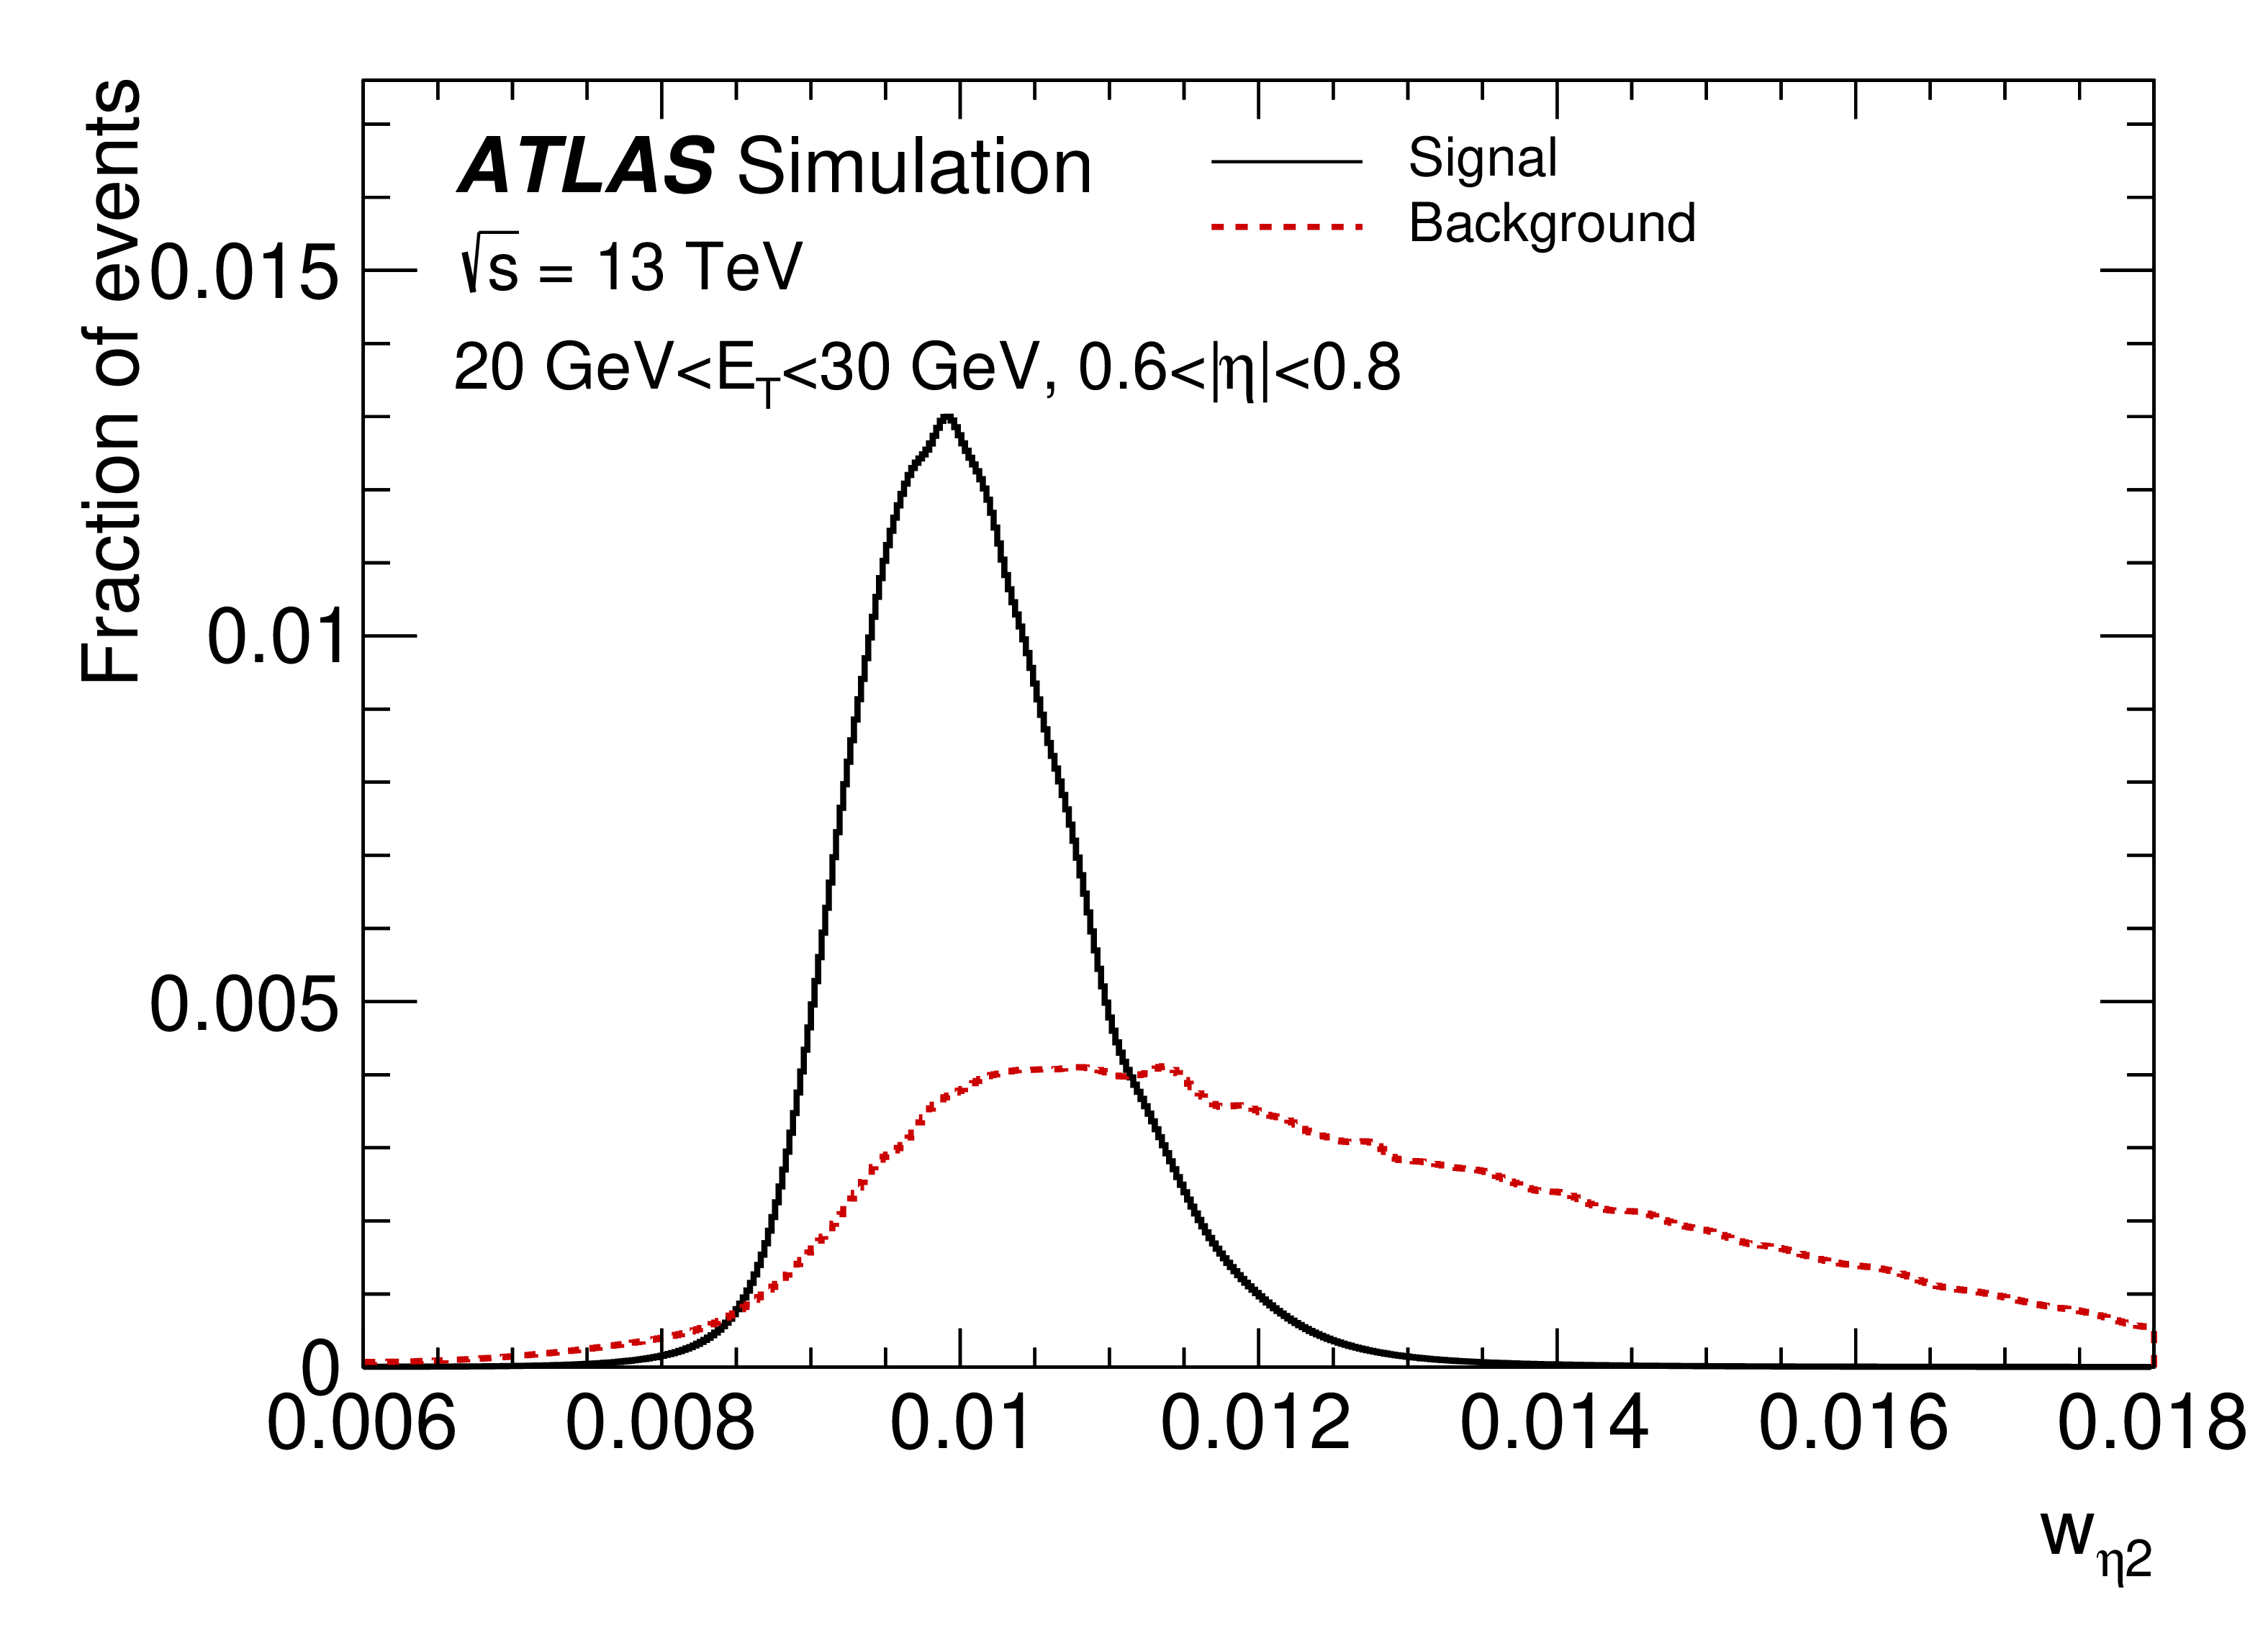
\includegraphics[width=1.0\textwidth]{figs/egamma/w_eta2.png} 
    \label{fig:egamma:weta2}
  \end{subfigure}
  \hfill
  \begin{subfigure}[b]{0.495\textwidth}
    \centering
    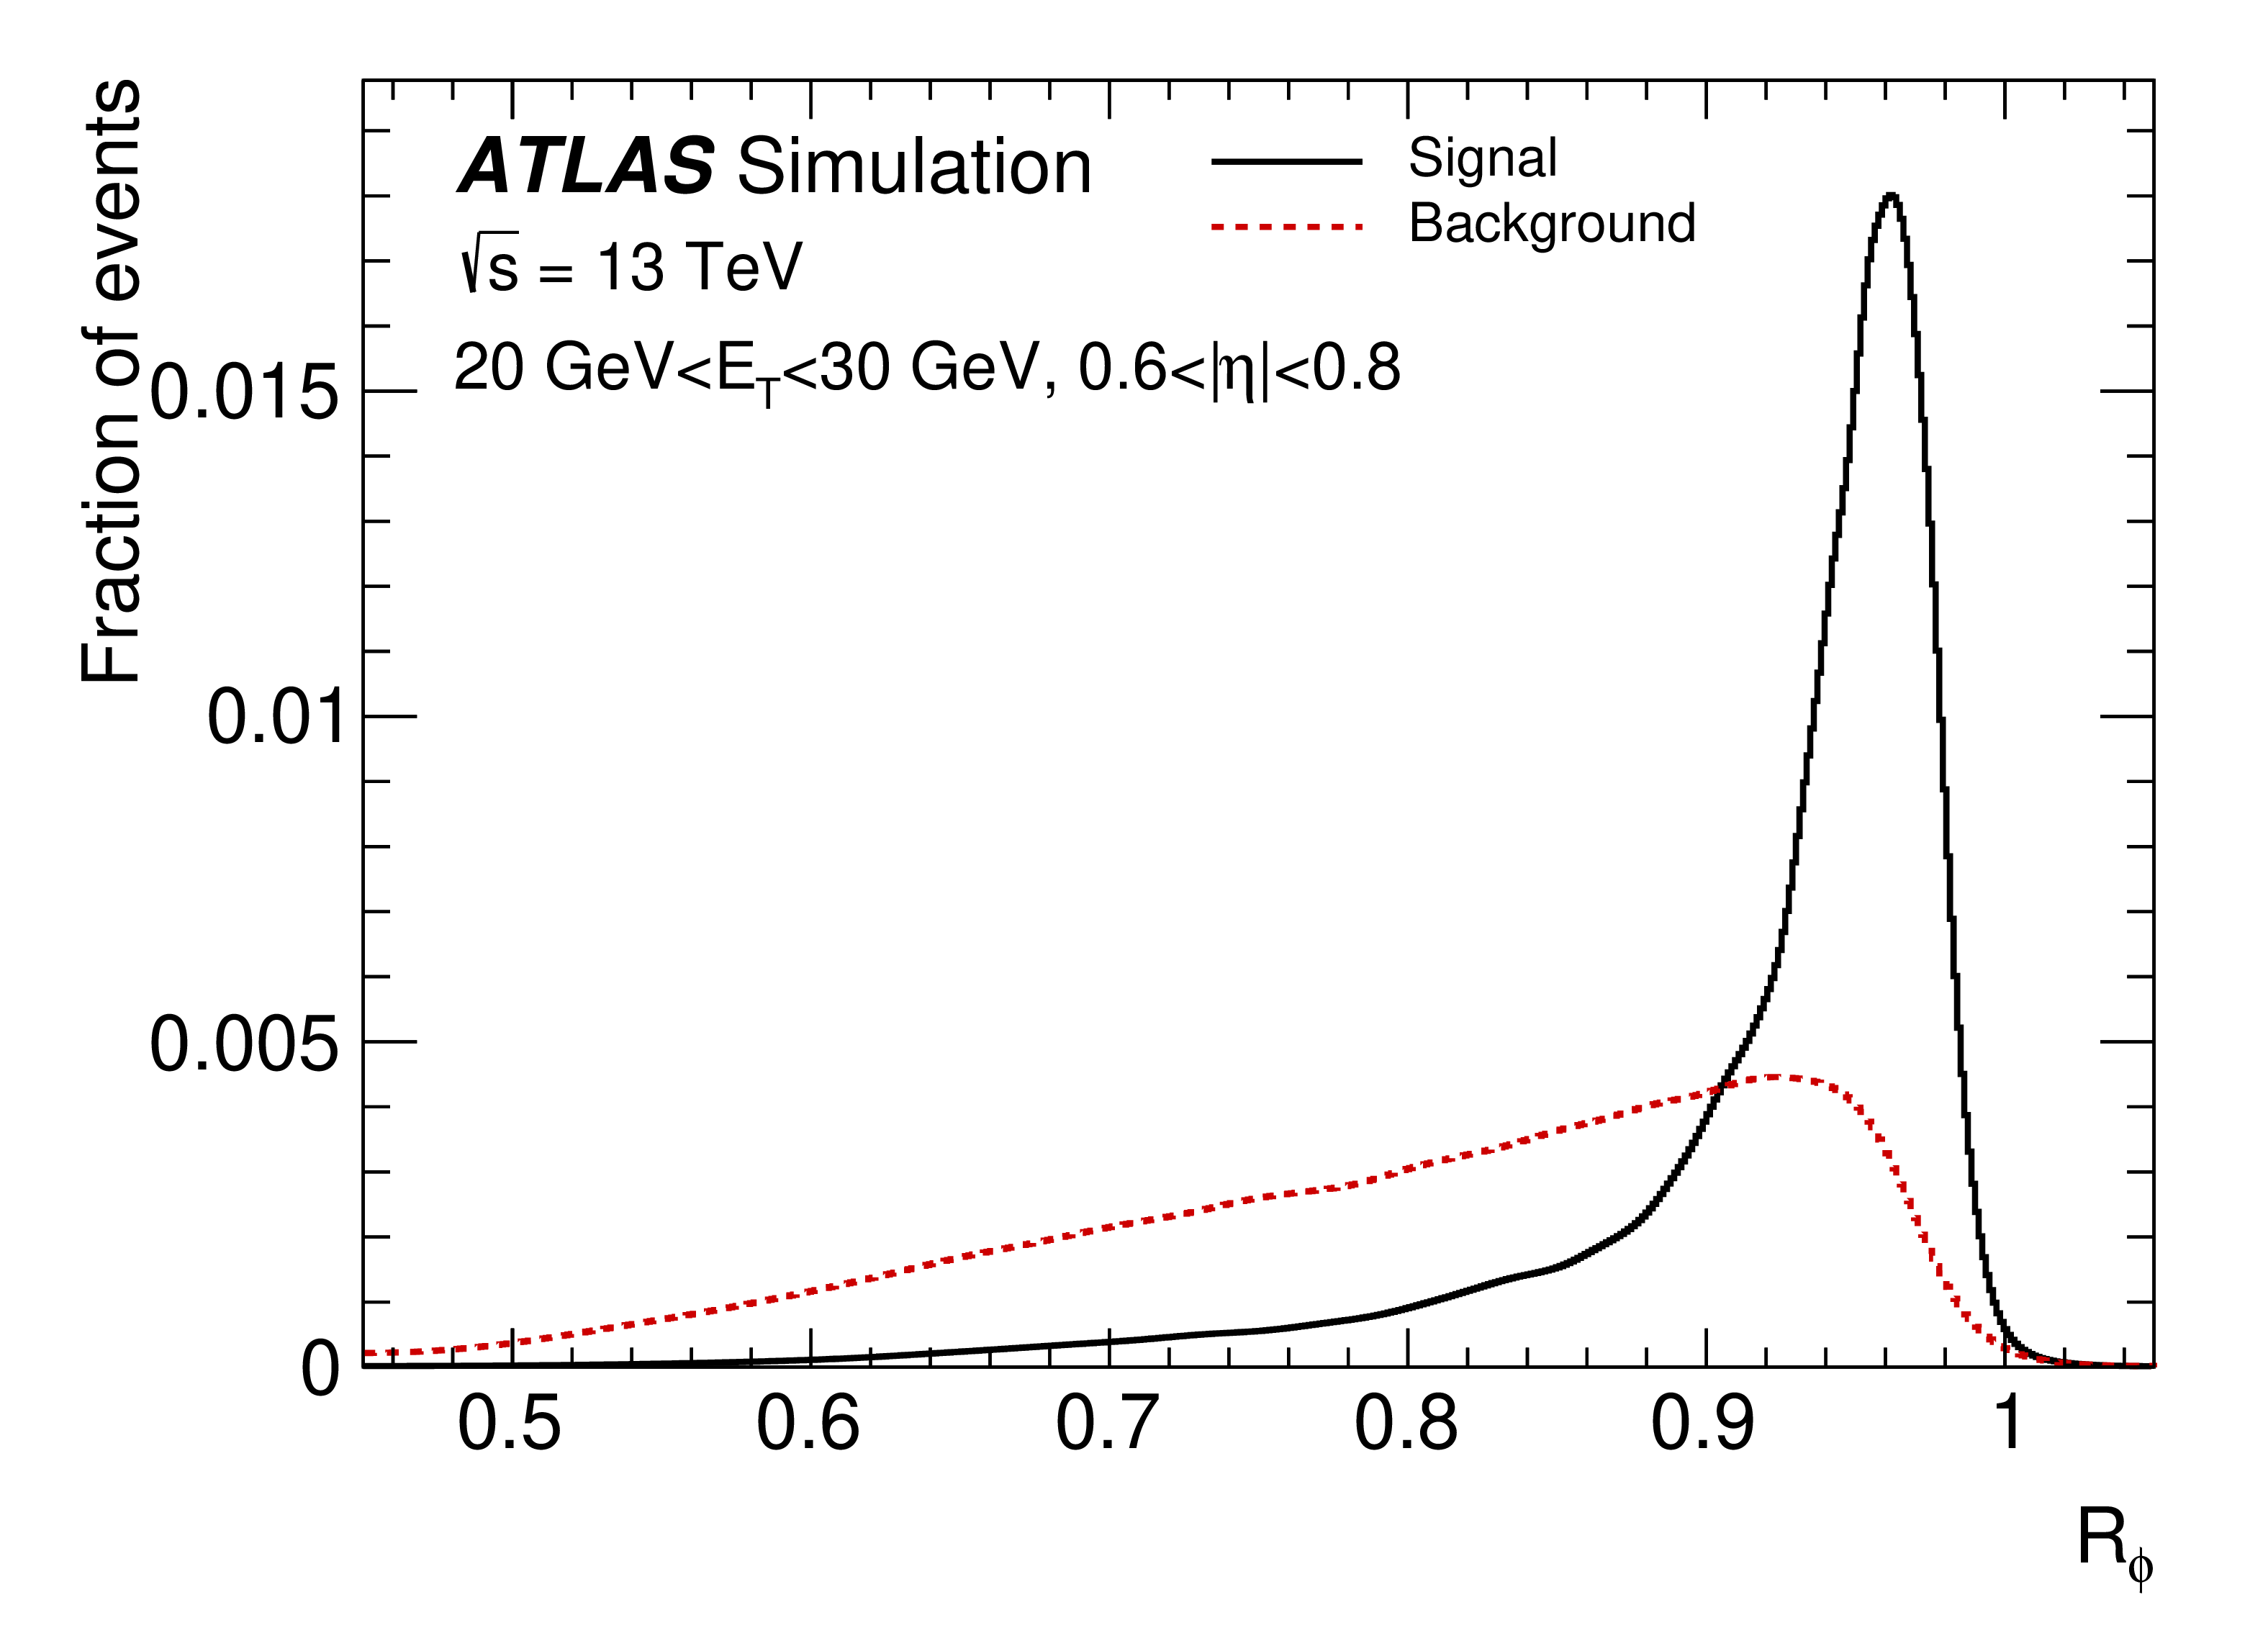
\includegraphics[width=1.0\textwidth]{figs/egamma/R_phi.png} 
    \label{fig:egamma:Rphi}
  \end{subfigure}
  \hfill
  \begin{subfigure}[b]{0.495\textwidth}
    \centering
    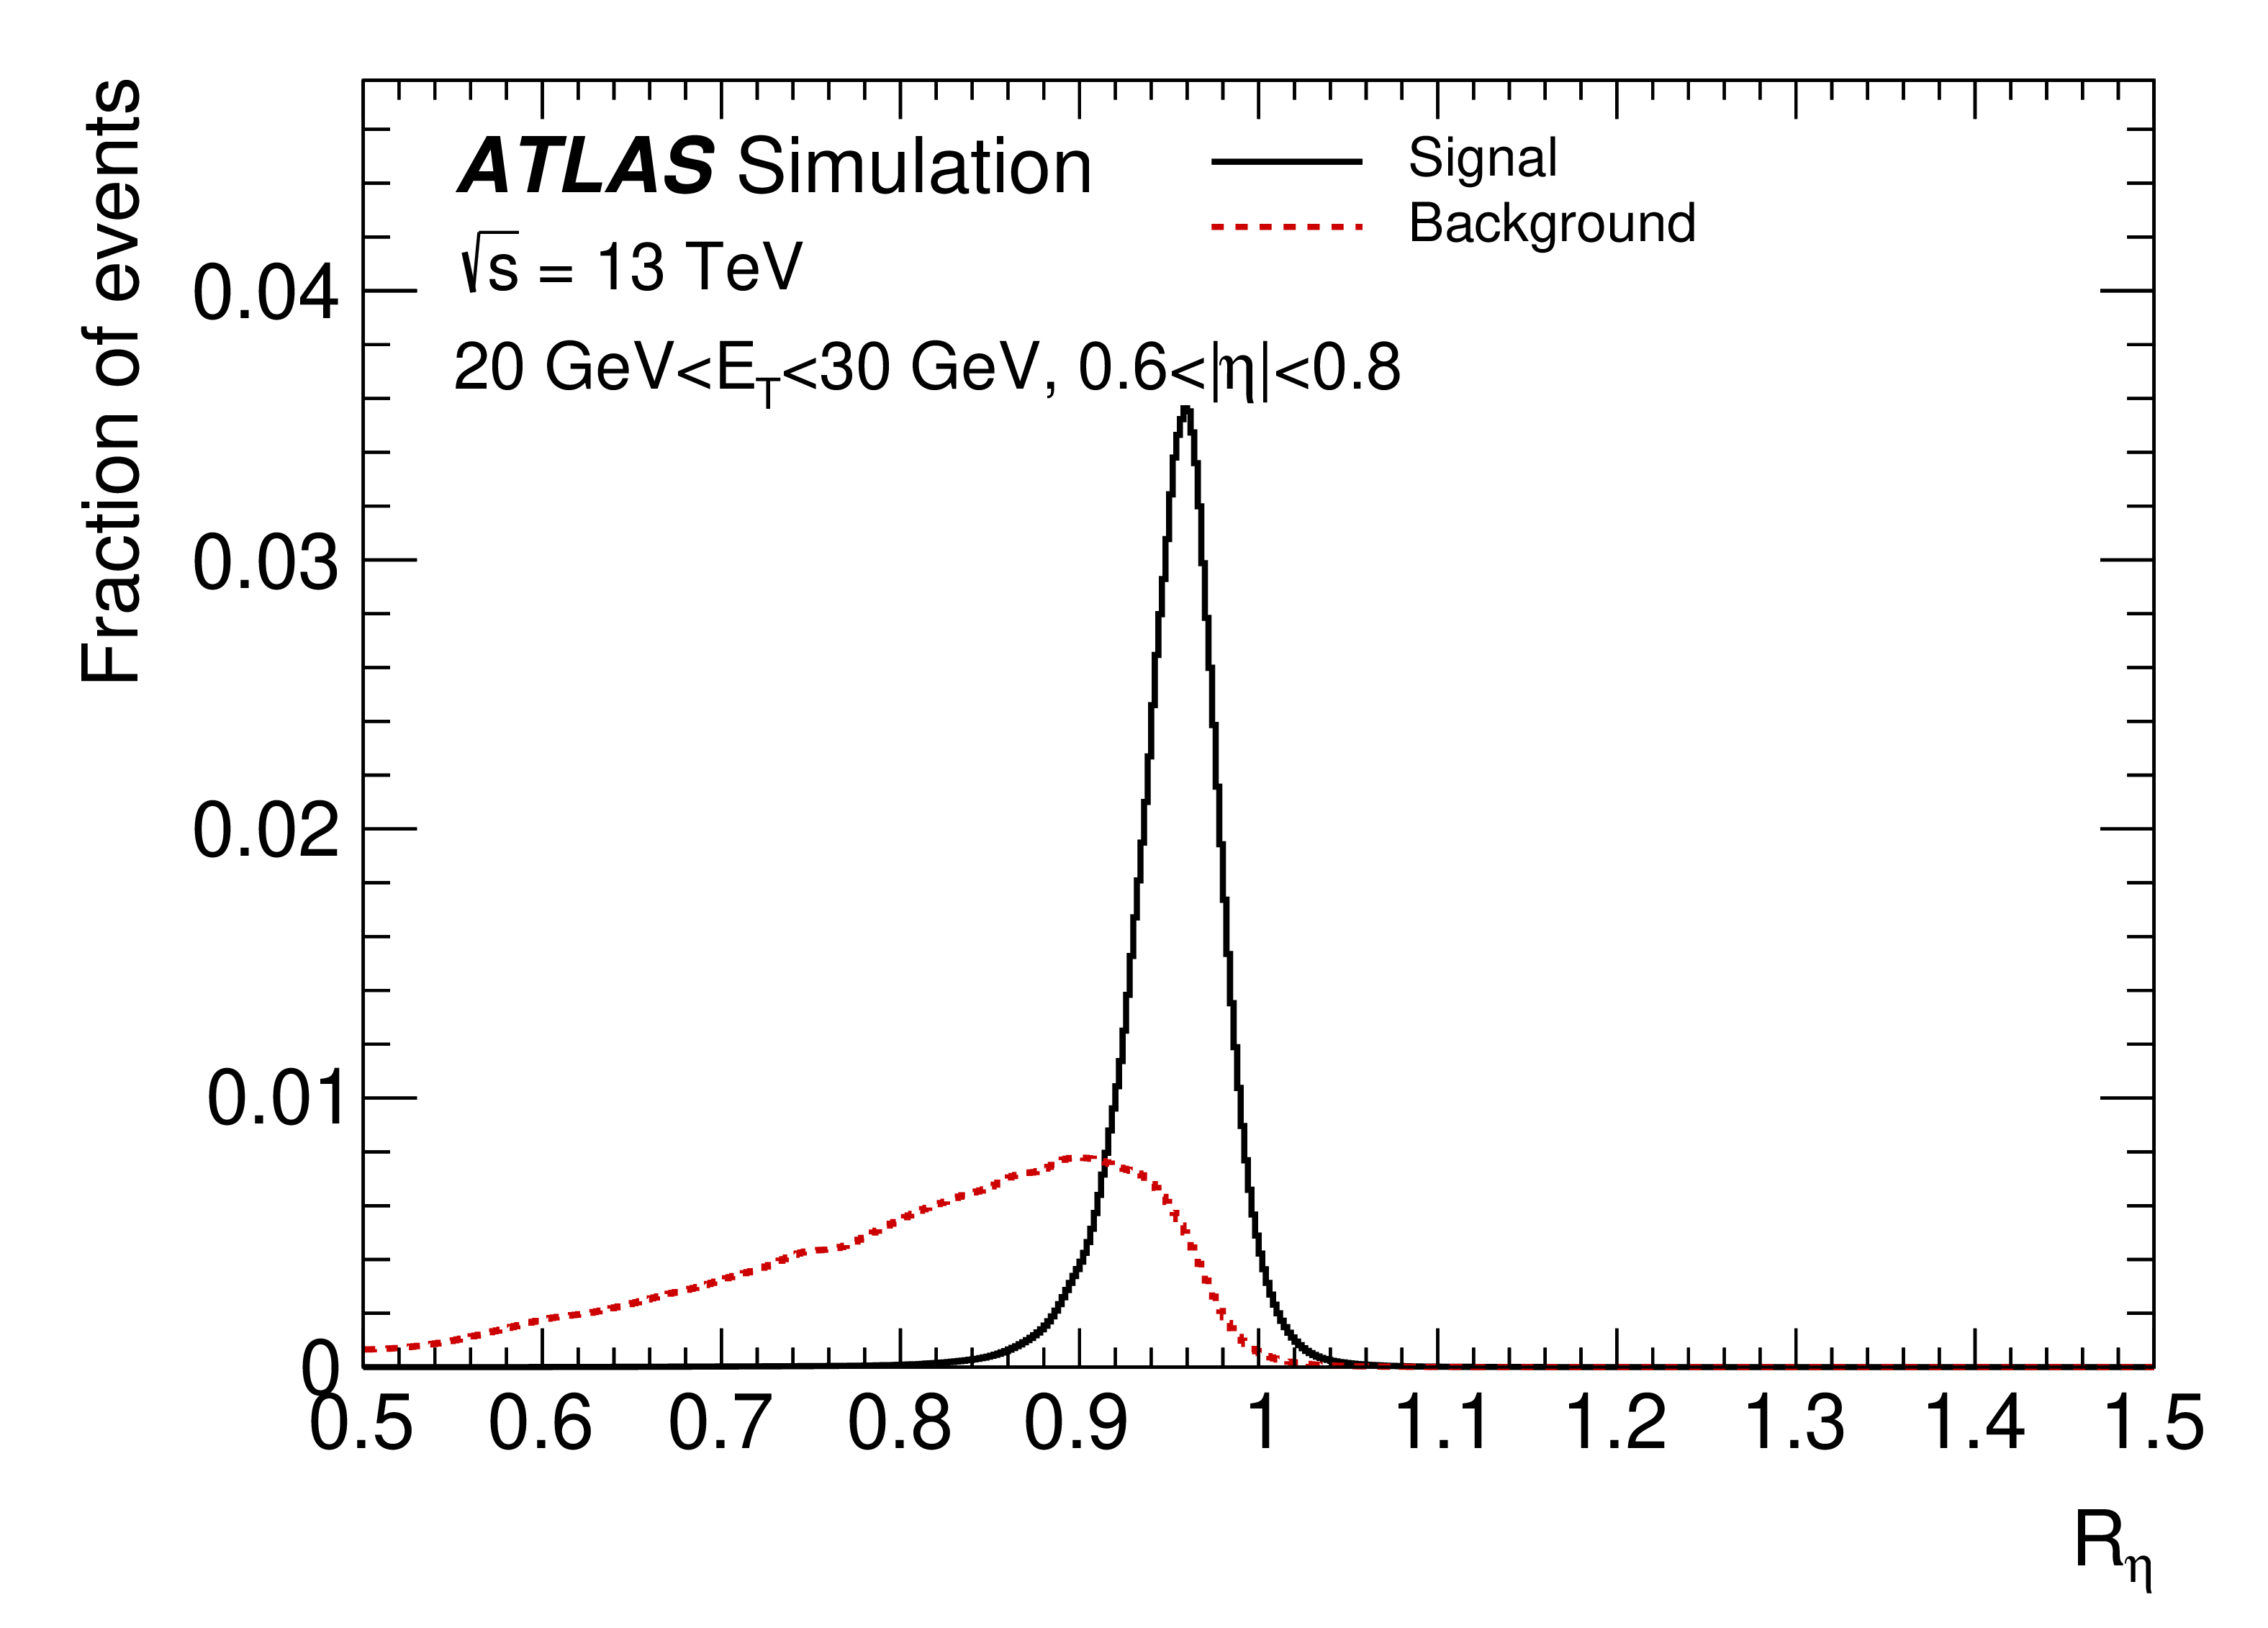
\includegraphics[width=1.0\textwidth]{figs/egamma/R_eta.png} 
    \label{fig:egamma:Reta}
  \end{subfigure}
  \hfill
  \begin{subfigure}[b]{0.495\textwidth}
    \centering
    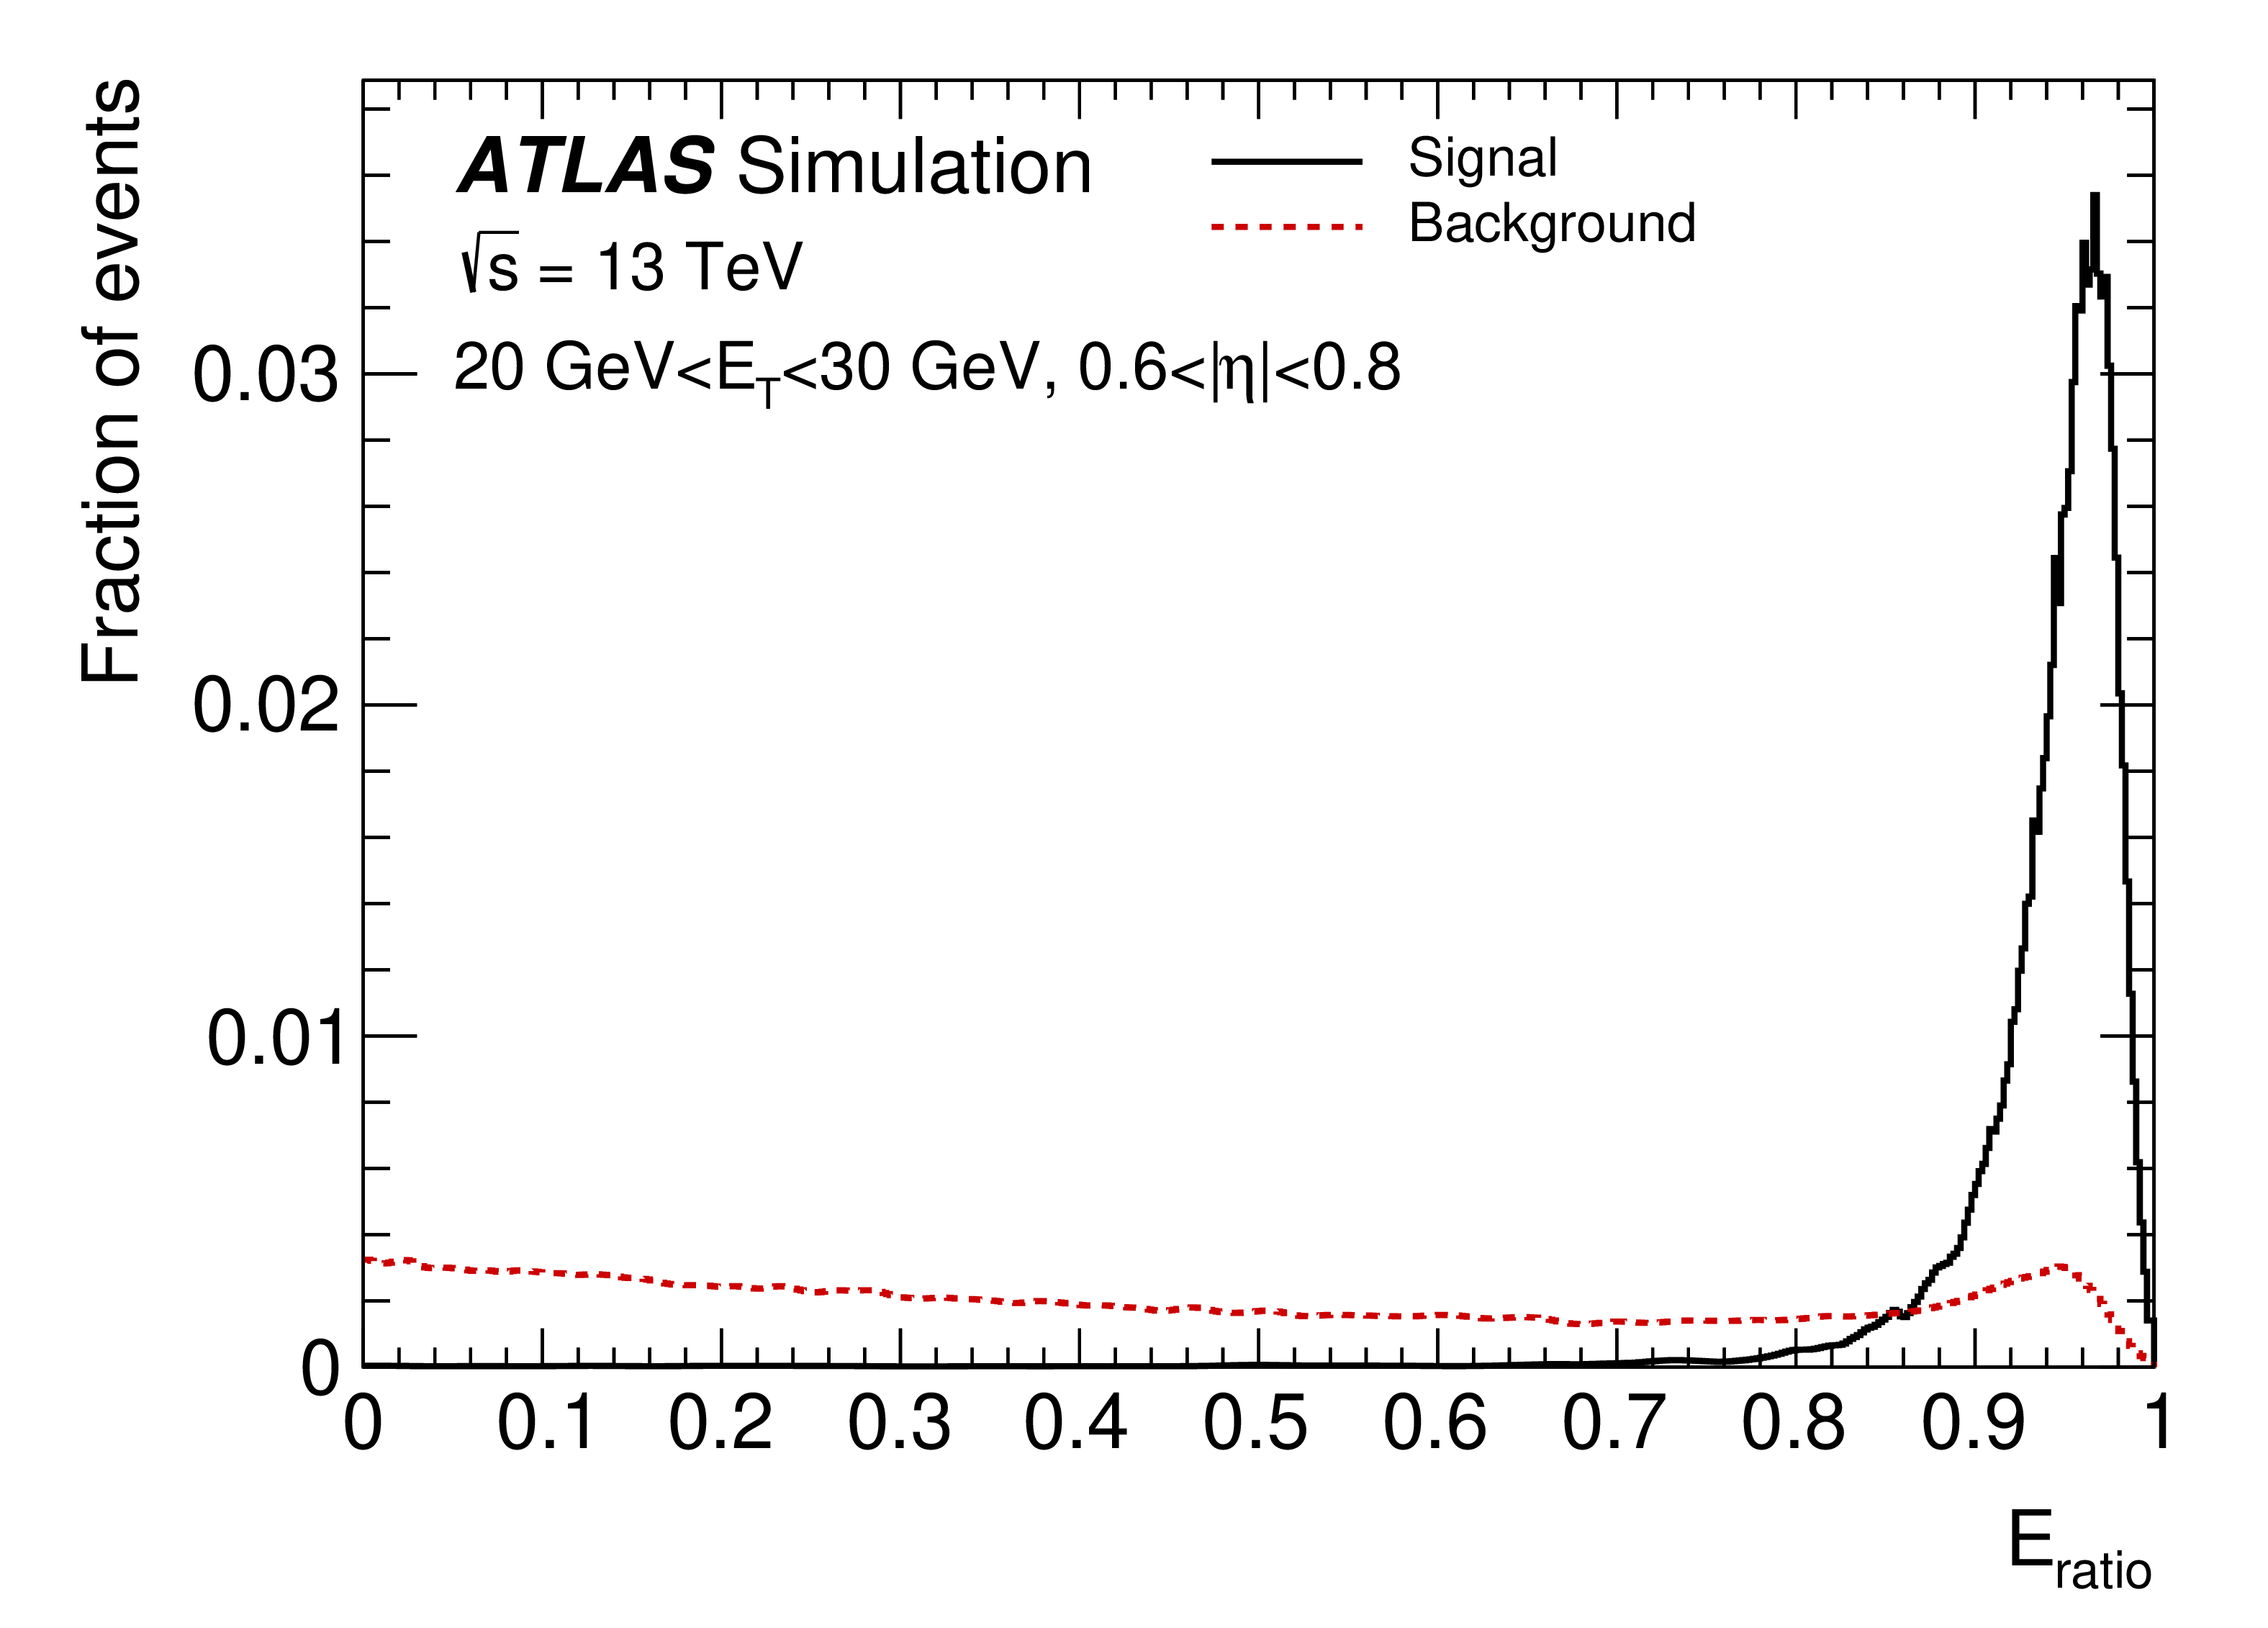
\includegraphics[width=1.0\textwidth]{figs/egamma/E_ratio.png} 
    \label{fig:egamma:Eratio}
  \end{subfigure}
  \hfill
  
  \caption[Example distributions of the calorimeter variables \rhadone, \fIII, and \fI.]{Example distributions of the calorimeter variables \rhadone, \fIII, and \fI.
    Defined in Table~\ref{tab:IDcuts} are shown for a typical \et/$\eta$ bin, 20~\GeV $<$ \et\ $<$ 30~\GeV and $0.6<|\eta|<0.8$.
    %that would be inefficient if used in a cut-based identification, but which, nonetheless, have significant discriminating power against background and, therefore, can be used to improve a LH-based identification.
    The red-dashed distribution is determined from a background simulation sample and the black-line distribution is determined from a \Zee simulation sample.
    These distributions are for reconstructed electron candidates before applying any identification.
    They are smoothed using an adaptive KDE and have been corrected for offsets or differences in widths between the distributions in data and simulation 
    %as described in Section~\ref{sec:egamma:LHpdfs}
    ~\cite{Aaboud:2019ynx}.
}
\label{fig:egamma:calorimeterWidth_pdfs}
\end{figure}

\begin{figure}[hp]
\centering
  \begin{subfigure}[b]{0.49\textwidth}
    \centering
    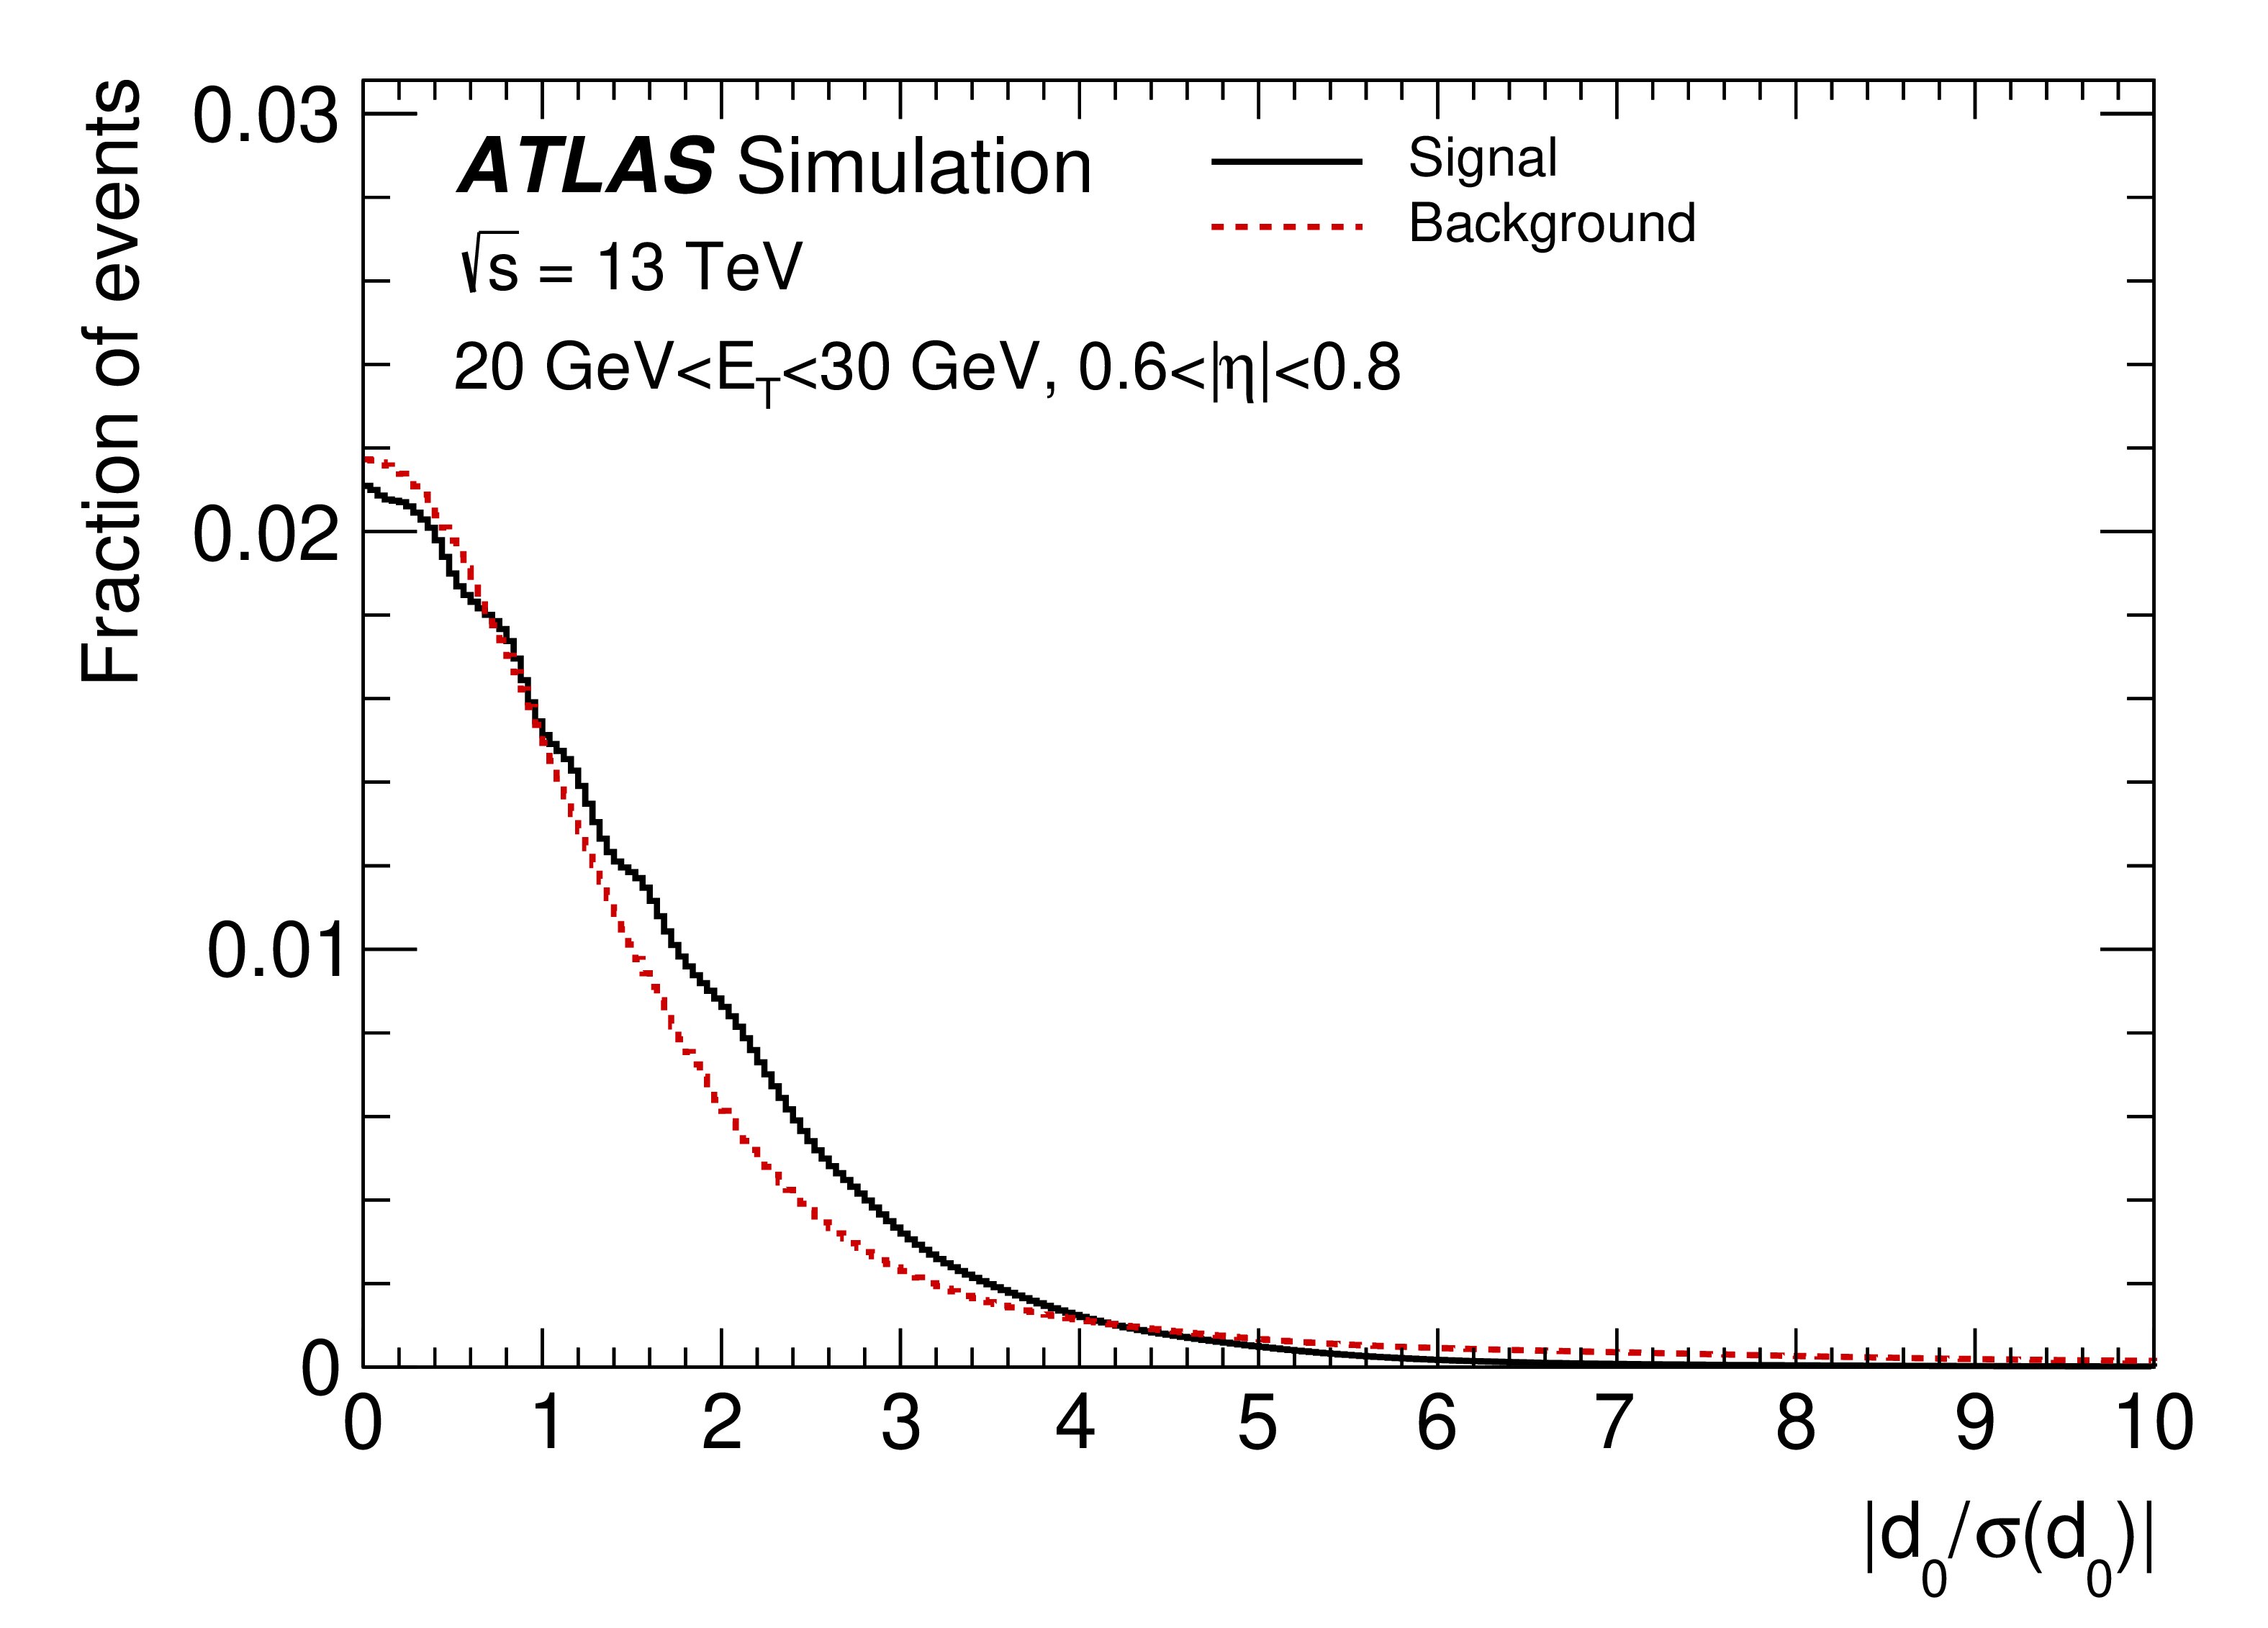
\includegraphics[width=1.0\textwidth]{figs/egamma/d0_sig.png} 
    \label{fig:egamma:d0_sig}
  \end{subfigure}
  \hfill
  \begin{subfigure}[b]{0.49\textwidth}
    \centering
    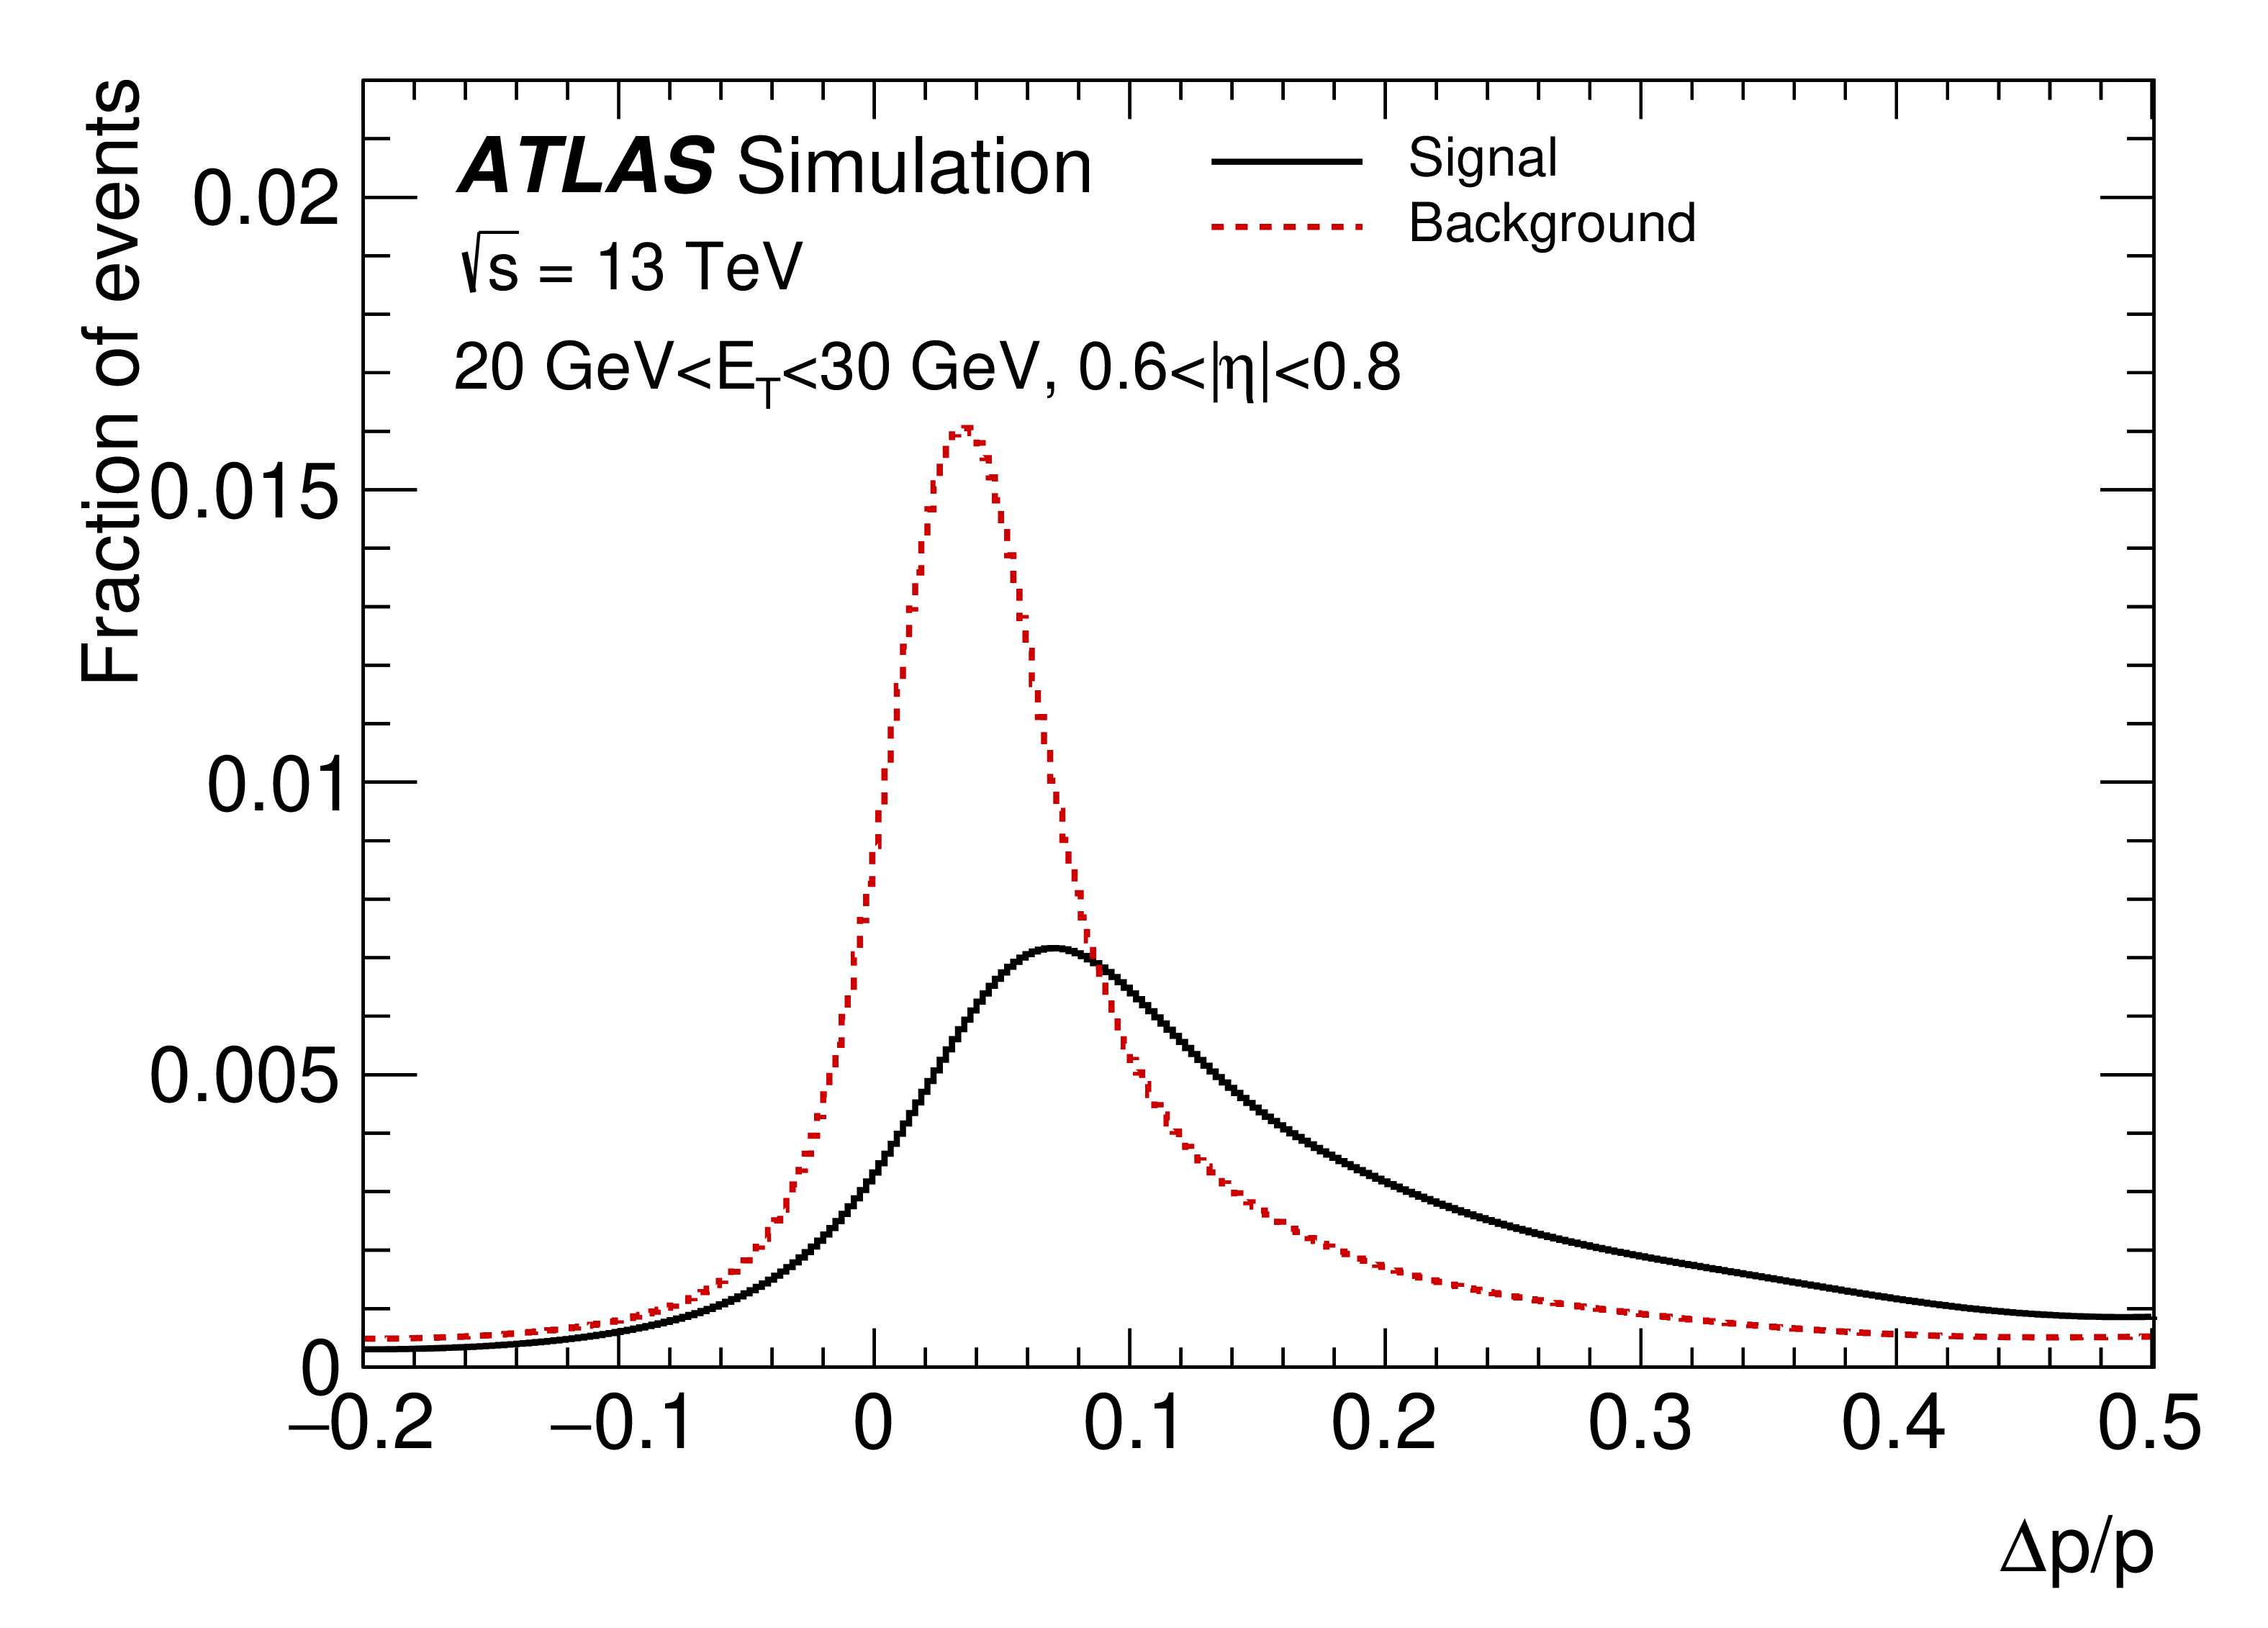
\includegraphics[width=1.0\textwidth]{figs/egamma/delatPoverp.png} 
    \label{fig:egamma:deltaPoverp}
  \end{subfigure}
  \hfill
  \begin{subfigure}[b]{0.49\textwidth}
    \centering
    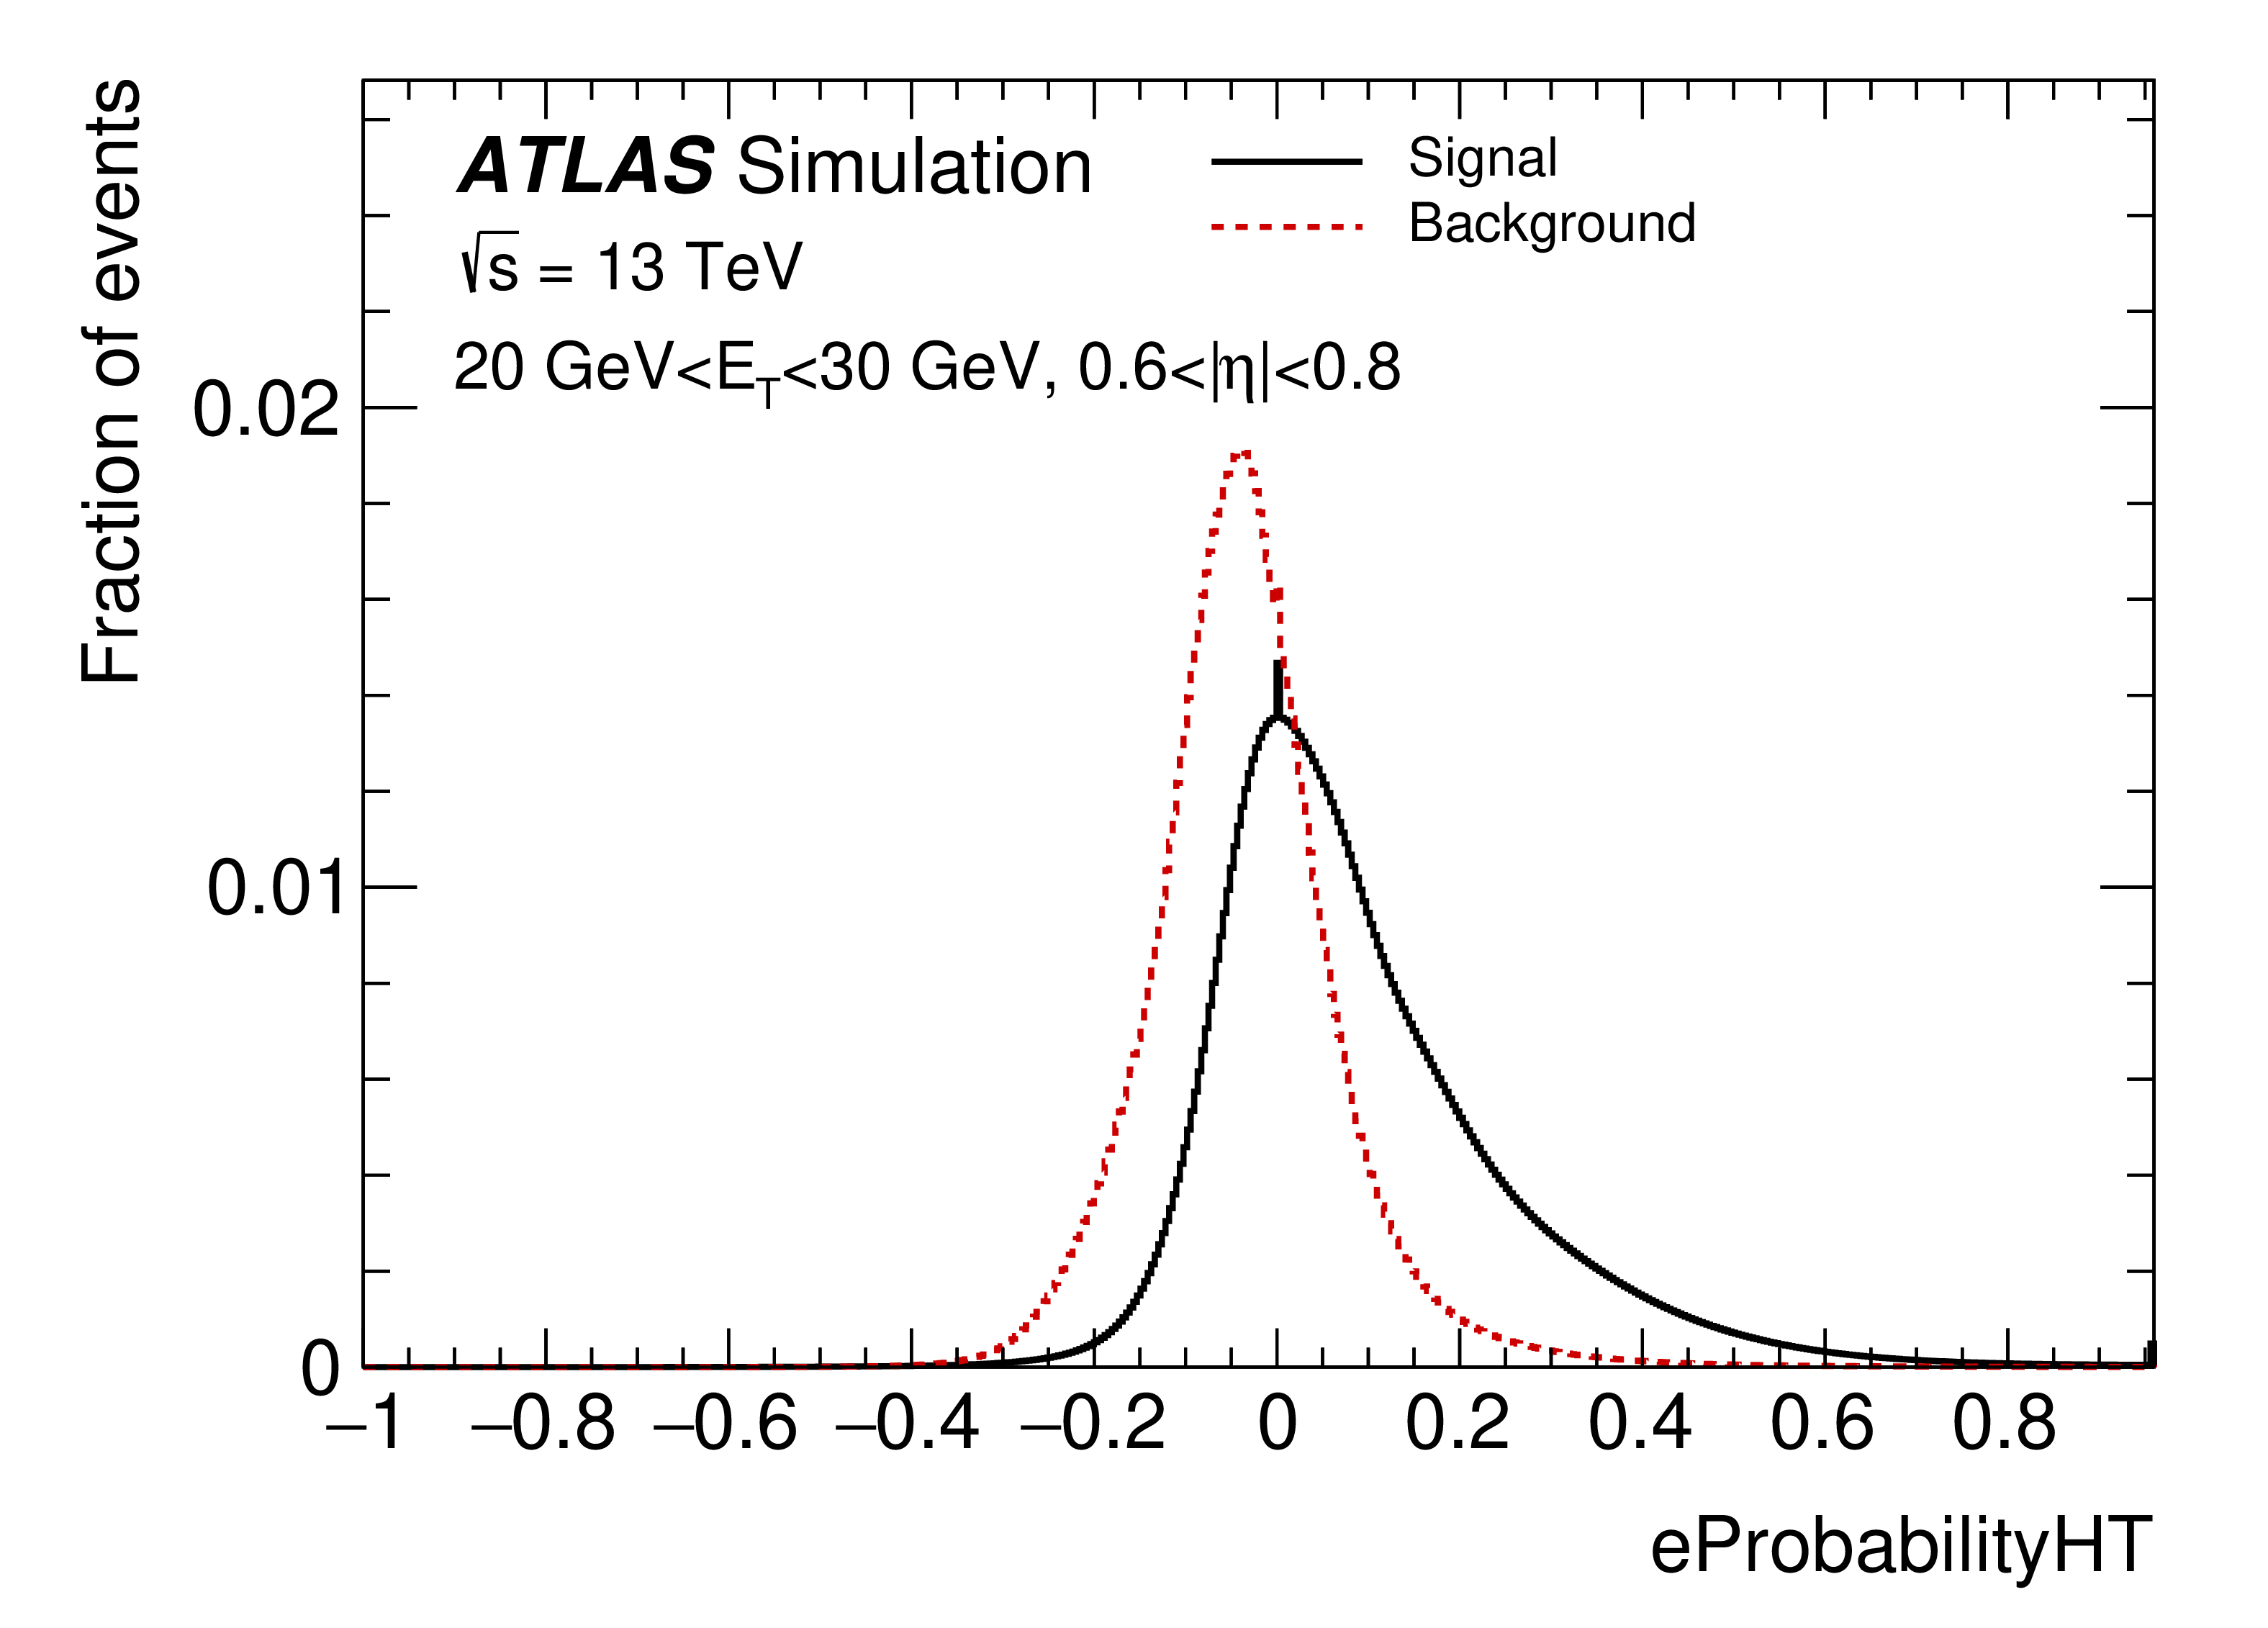
\includegraphics[width=1.0\textwidth]{figs/egamma/eProbHT.png} 
    \label{fig:egamma:eProbHT}
  \end{subfigure}
  \hfill
  \begin{subfigure}[b]{0.49\textwidth}
    \centering
    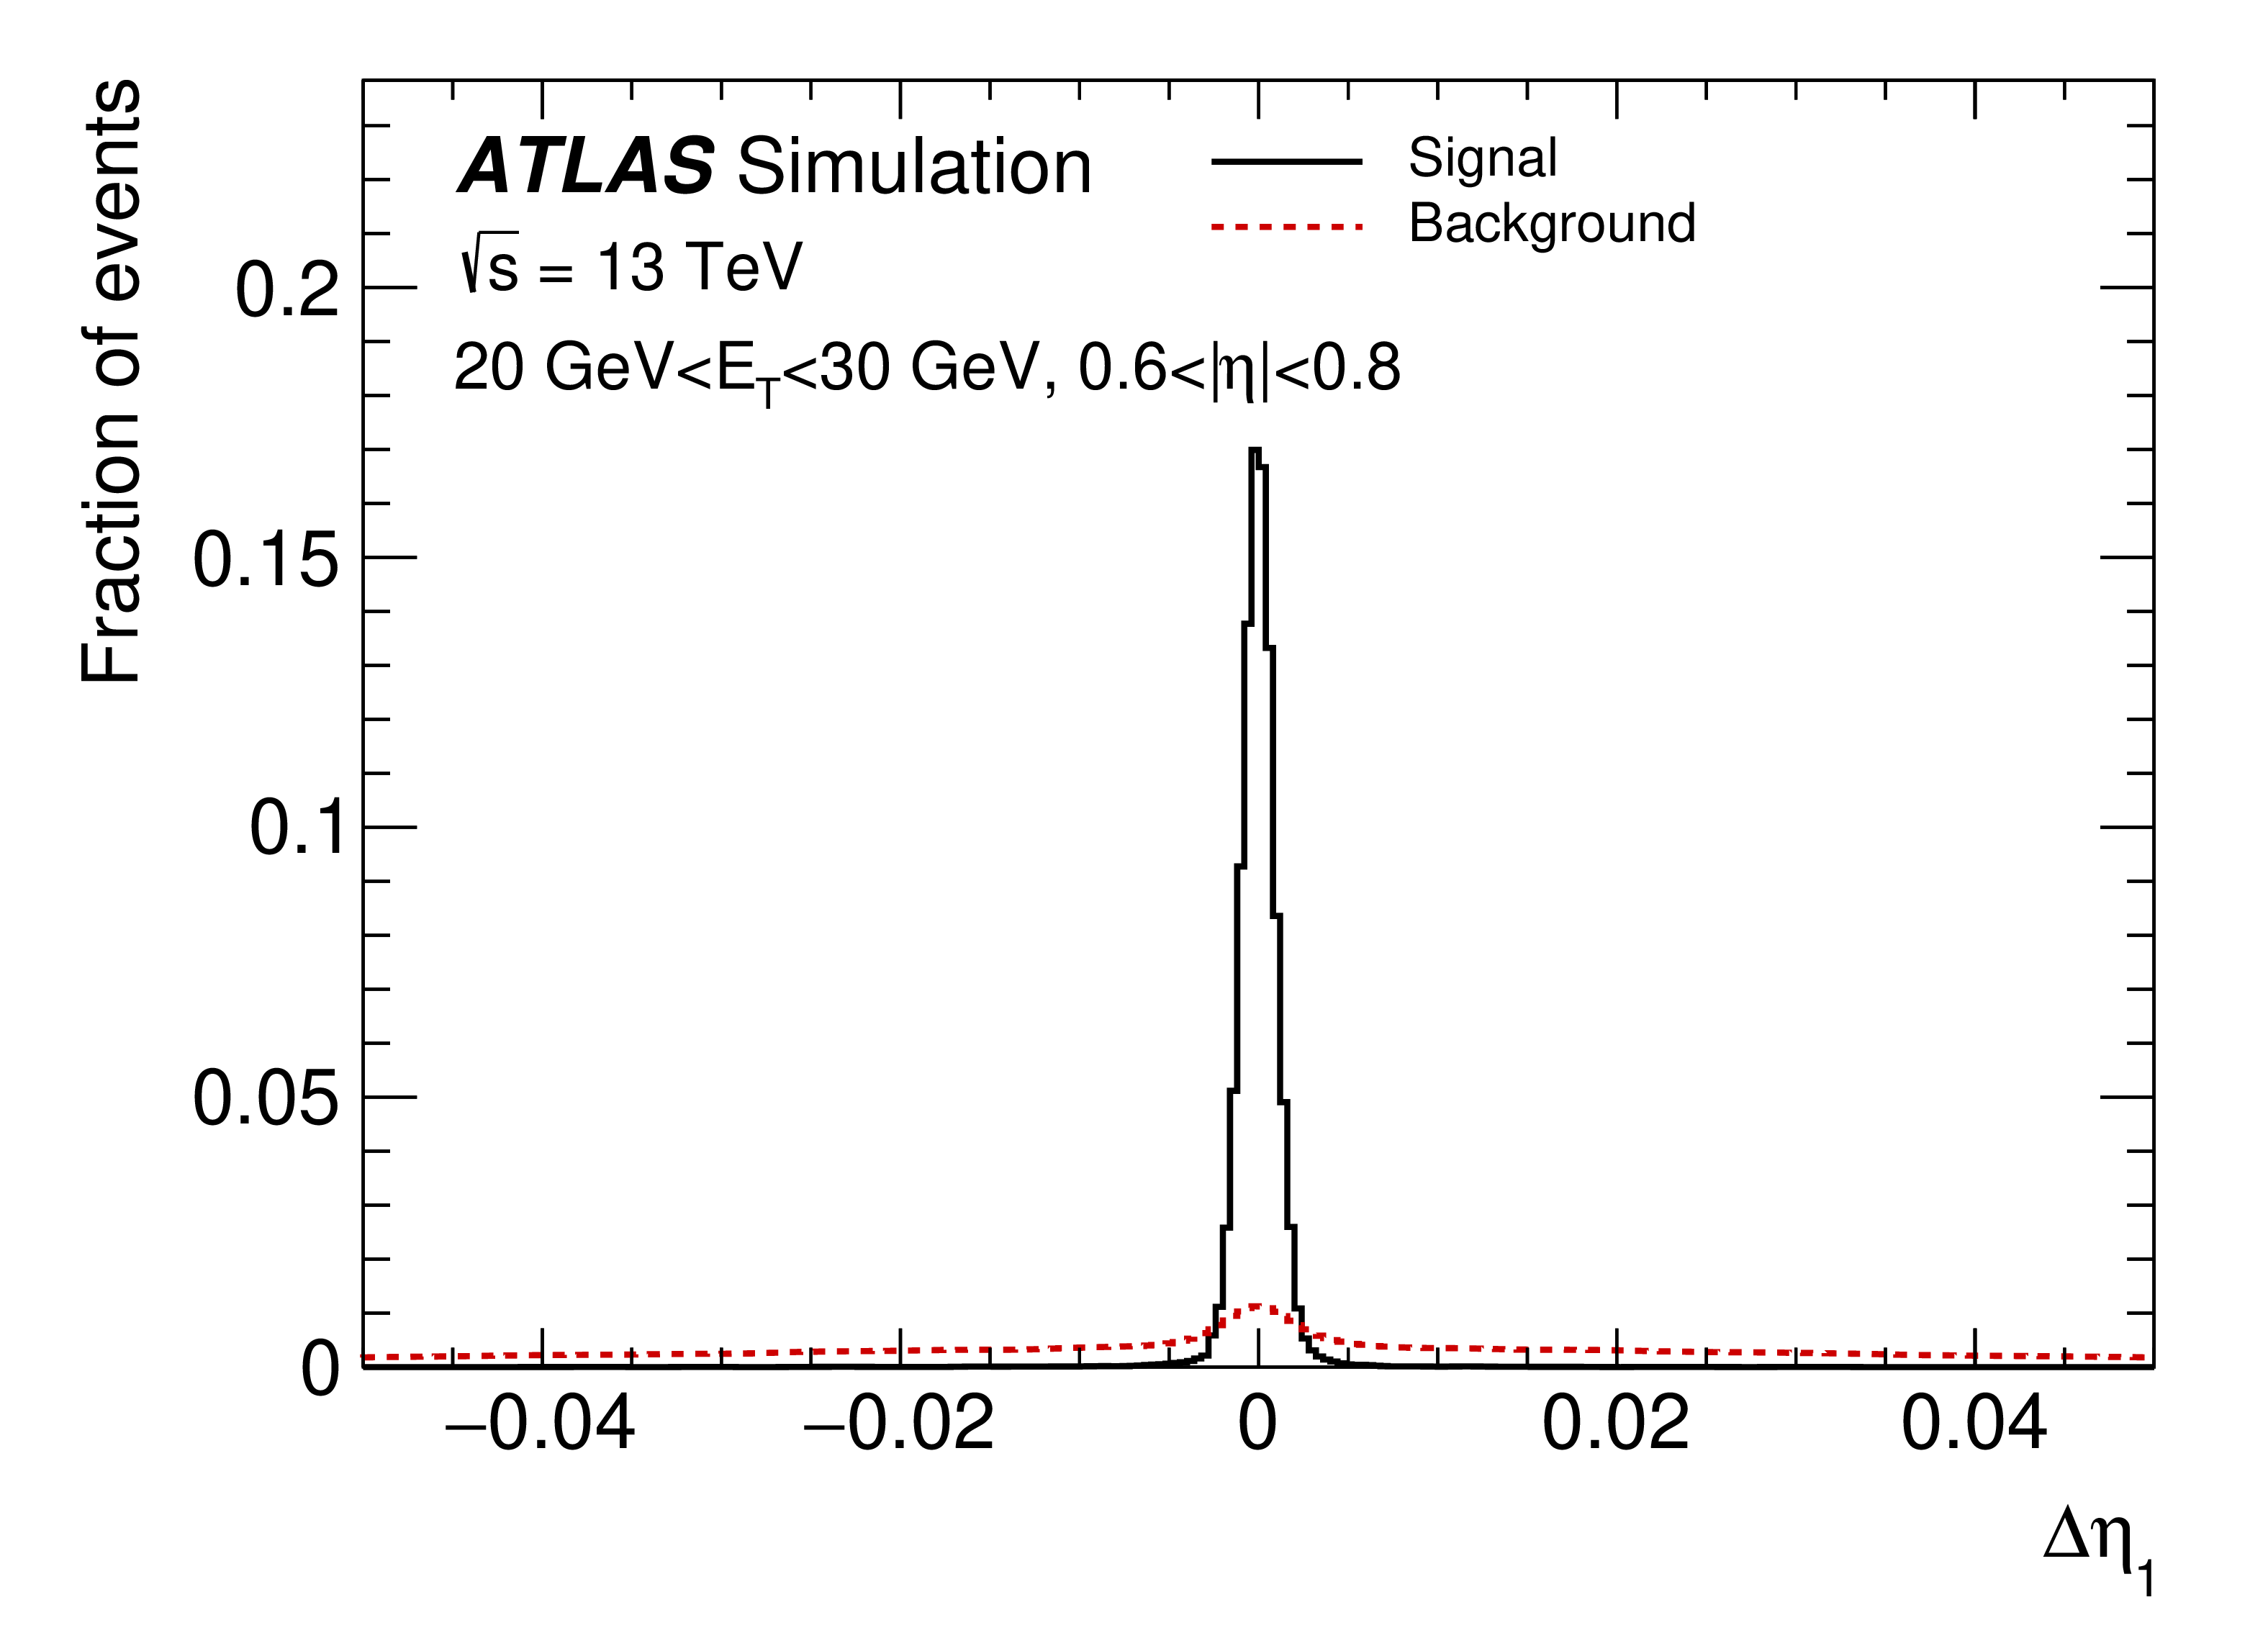
\includegraphics[width=1.0\textwidth]{figs/egamma/deltaEta_1.png} 
    \label{fig:egamma:deltaEta_1}
  \end{subfigure}
  \hfill
  \begin{subfigure}[b]{0.49\textwidth}
    \centering
    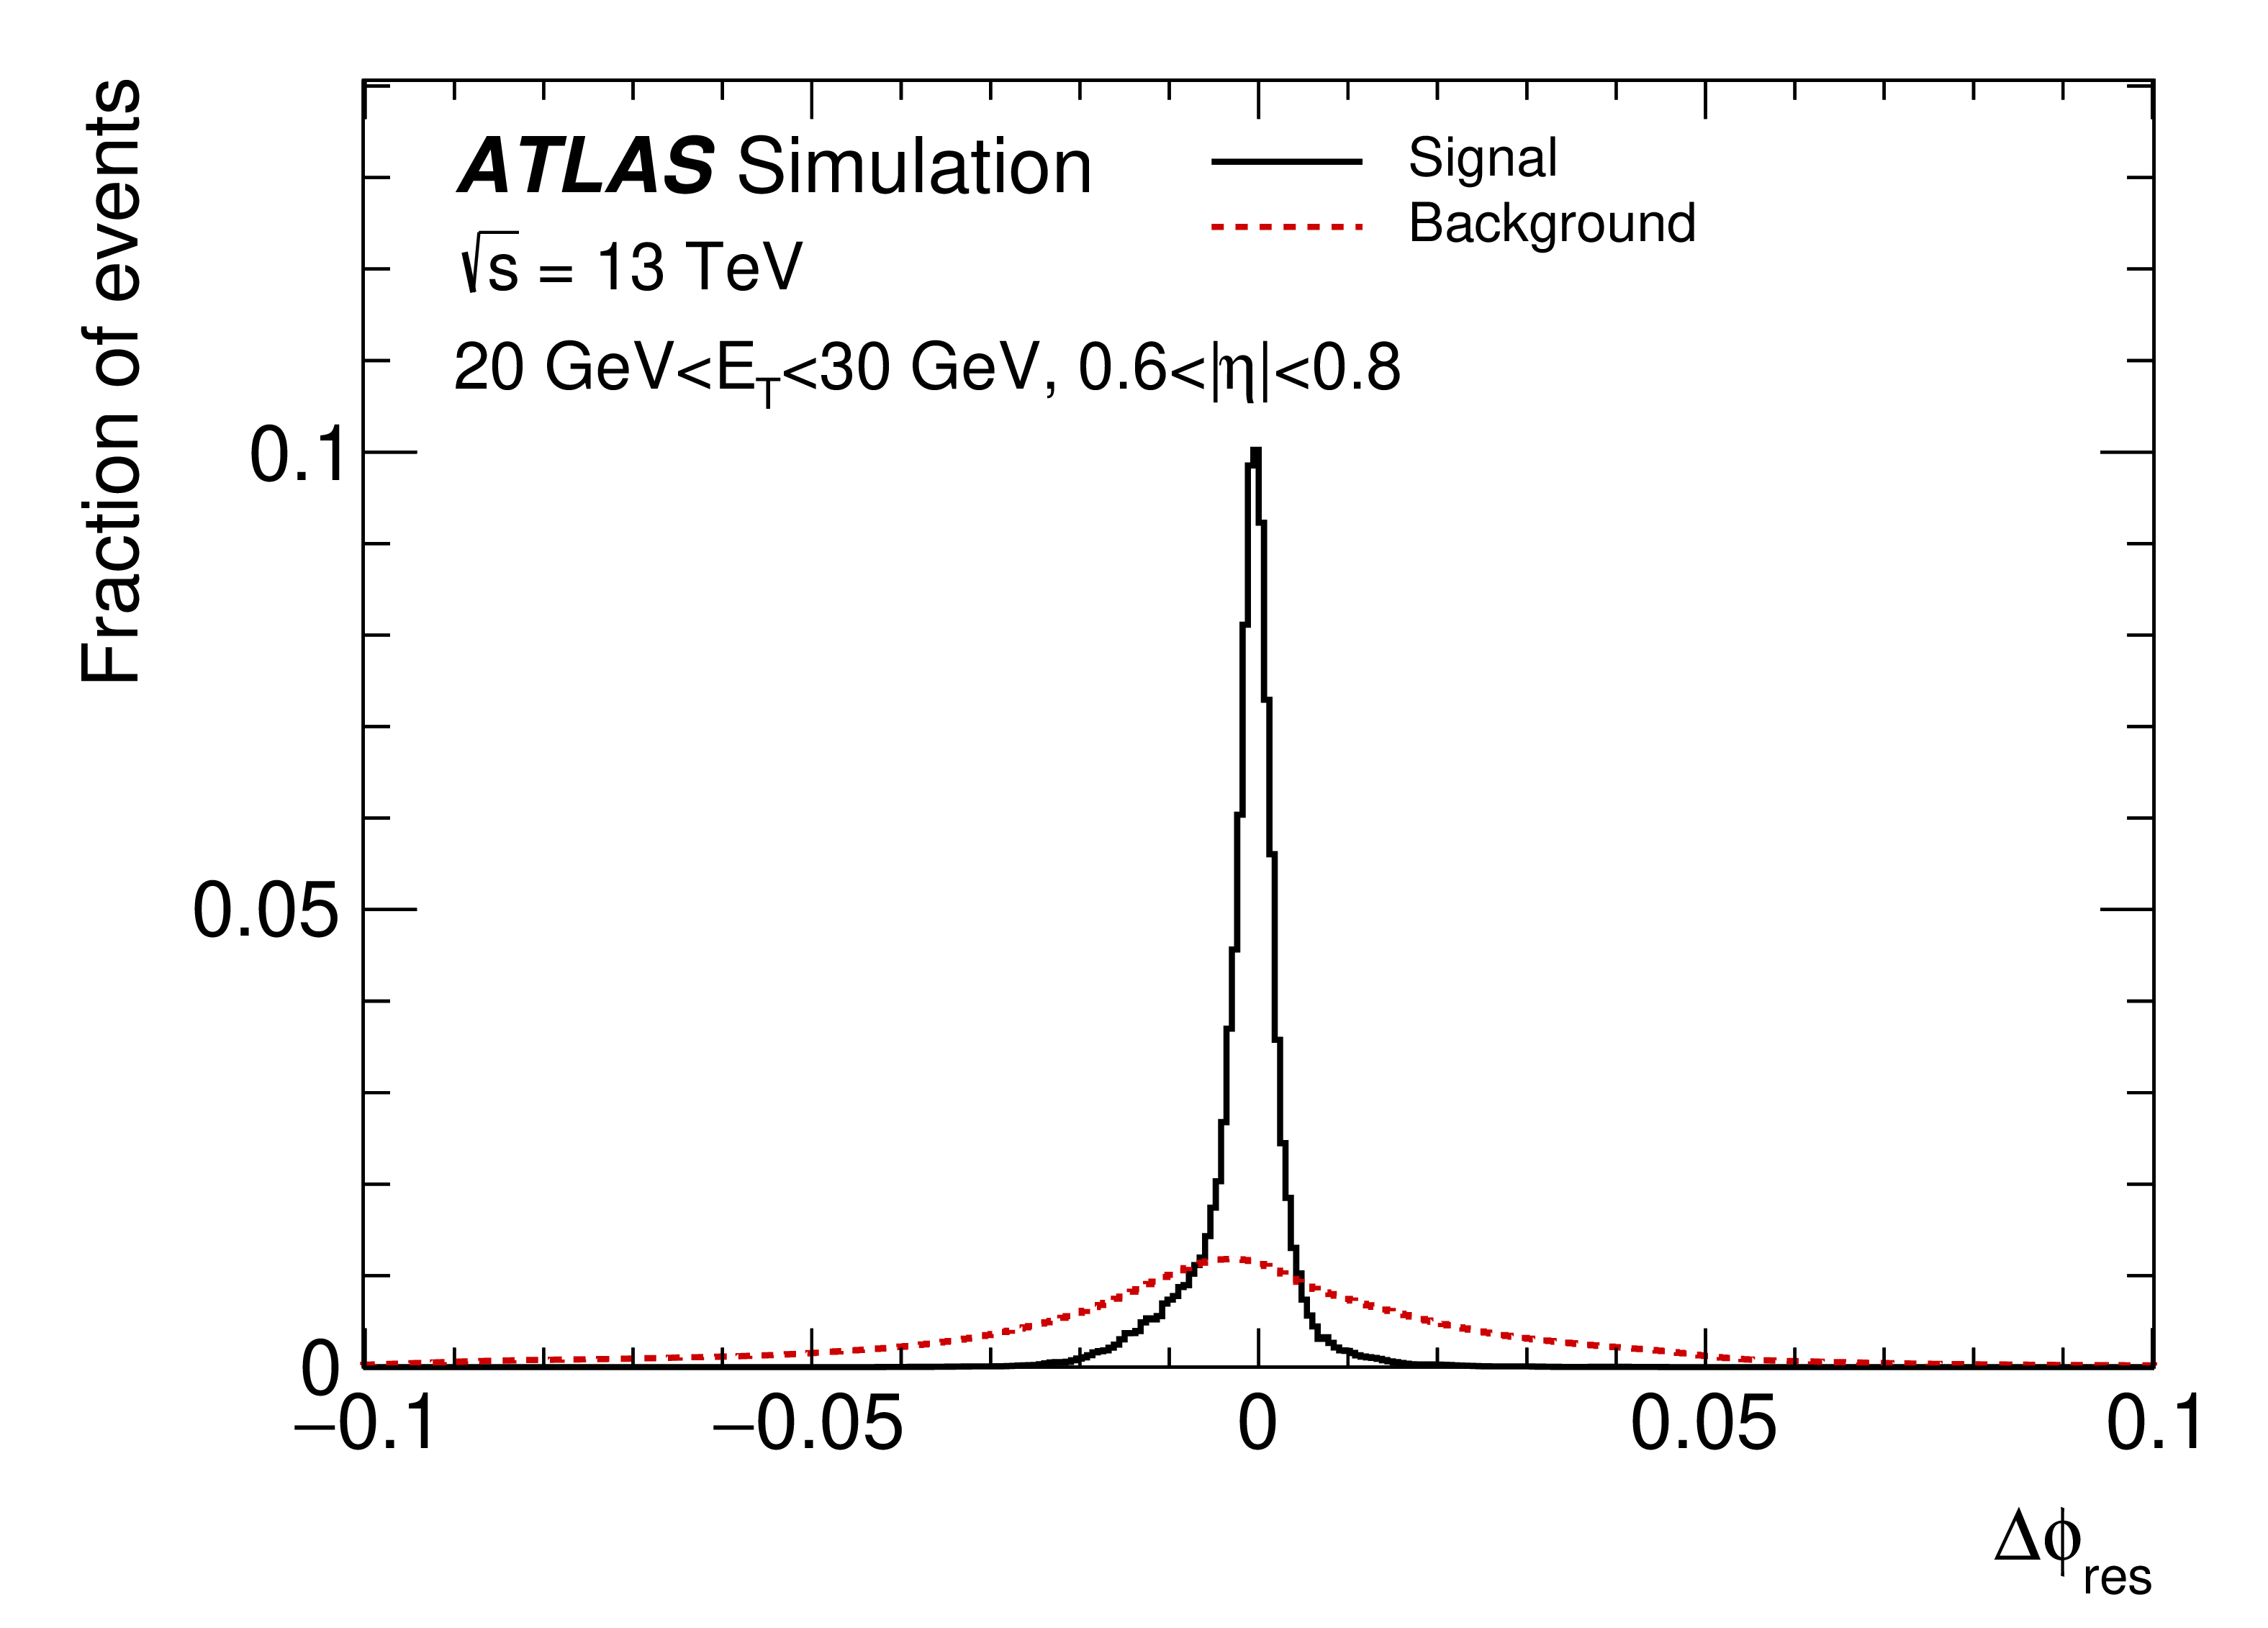
\includegraphics[width=1.0\textwidth]{figs/egamma/deltaPhi_res.png} 
    \label{fig:egamma:deltaPhi_res}
  \end{subfigure}
  \caption[Examples of distributions of tracking and track-cluster matching variables \dOSignificance, \deltapoverp, \TRTPID, \deltaeta, and \deltaphires.]{Examples of distributions of tracking and track-cluster matching variables \dOSignificance, \deltapoverp, \TRTPID, \deltaeta, and \deltaphires.
    All of which are defined in Table~\ref{tab:IDcuts} and shown for 20~\GeV $<$ \et\ $<$ 30~\GeV and $0.6<|\eta|<0.8$.
    %that would be inefficient if used in a cut-based identification, but which, nonetheless, have significant discriminating power against background and, therefore, can be used to improve a LH-based identification.
    The red-dashed distribution is determined from a background simulation sample and the black-line distribution is determined from a \Zee simulation sample.
    These distributions are for reconstructed electron candidates before applying any identification.
    They are smoothed using an adaptive KDE and have been corrected for offsets or differences in widths between the distributions in data and simulation
    %as described in Section~\ref{sec:egamma:LHpdfs}
    ~\cite{Aaboud:2019ynx}.
}
\label{fig:egamma:calorimeter_pdfs}
\end{figure}
\begin{figure}[tbp]
  \centering
  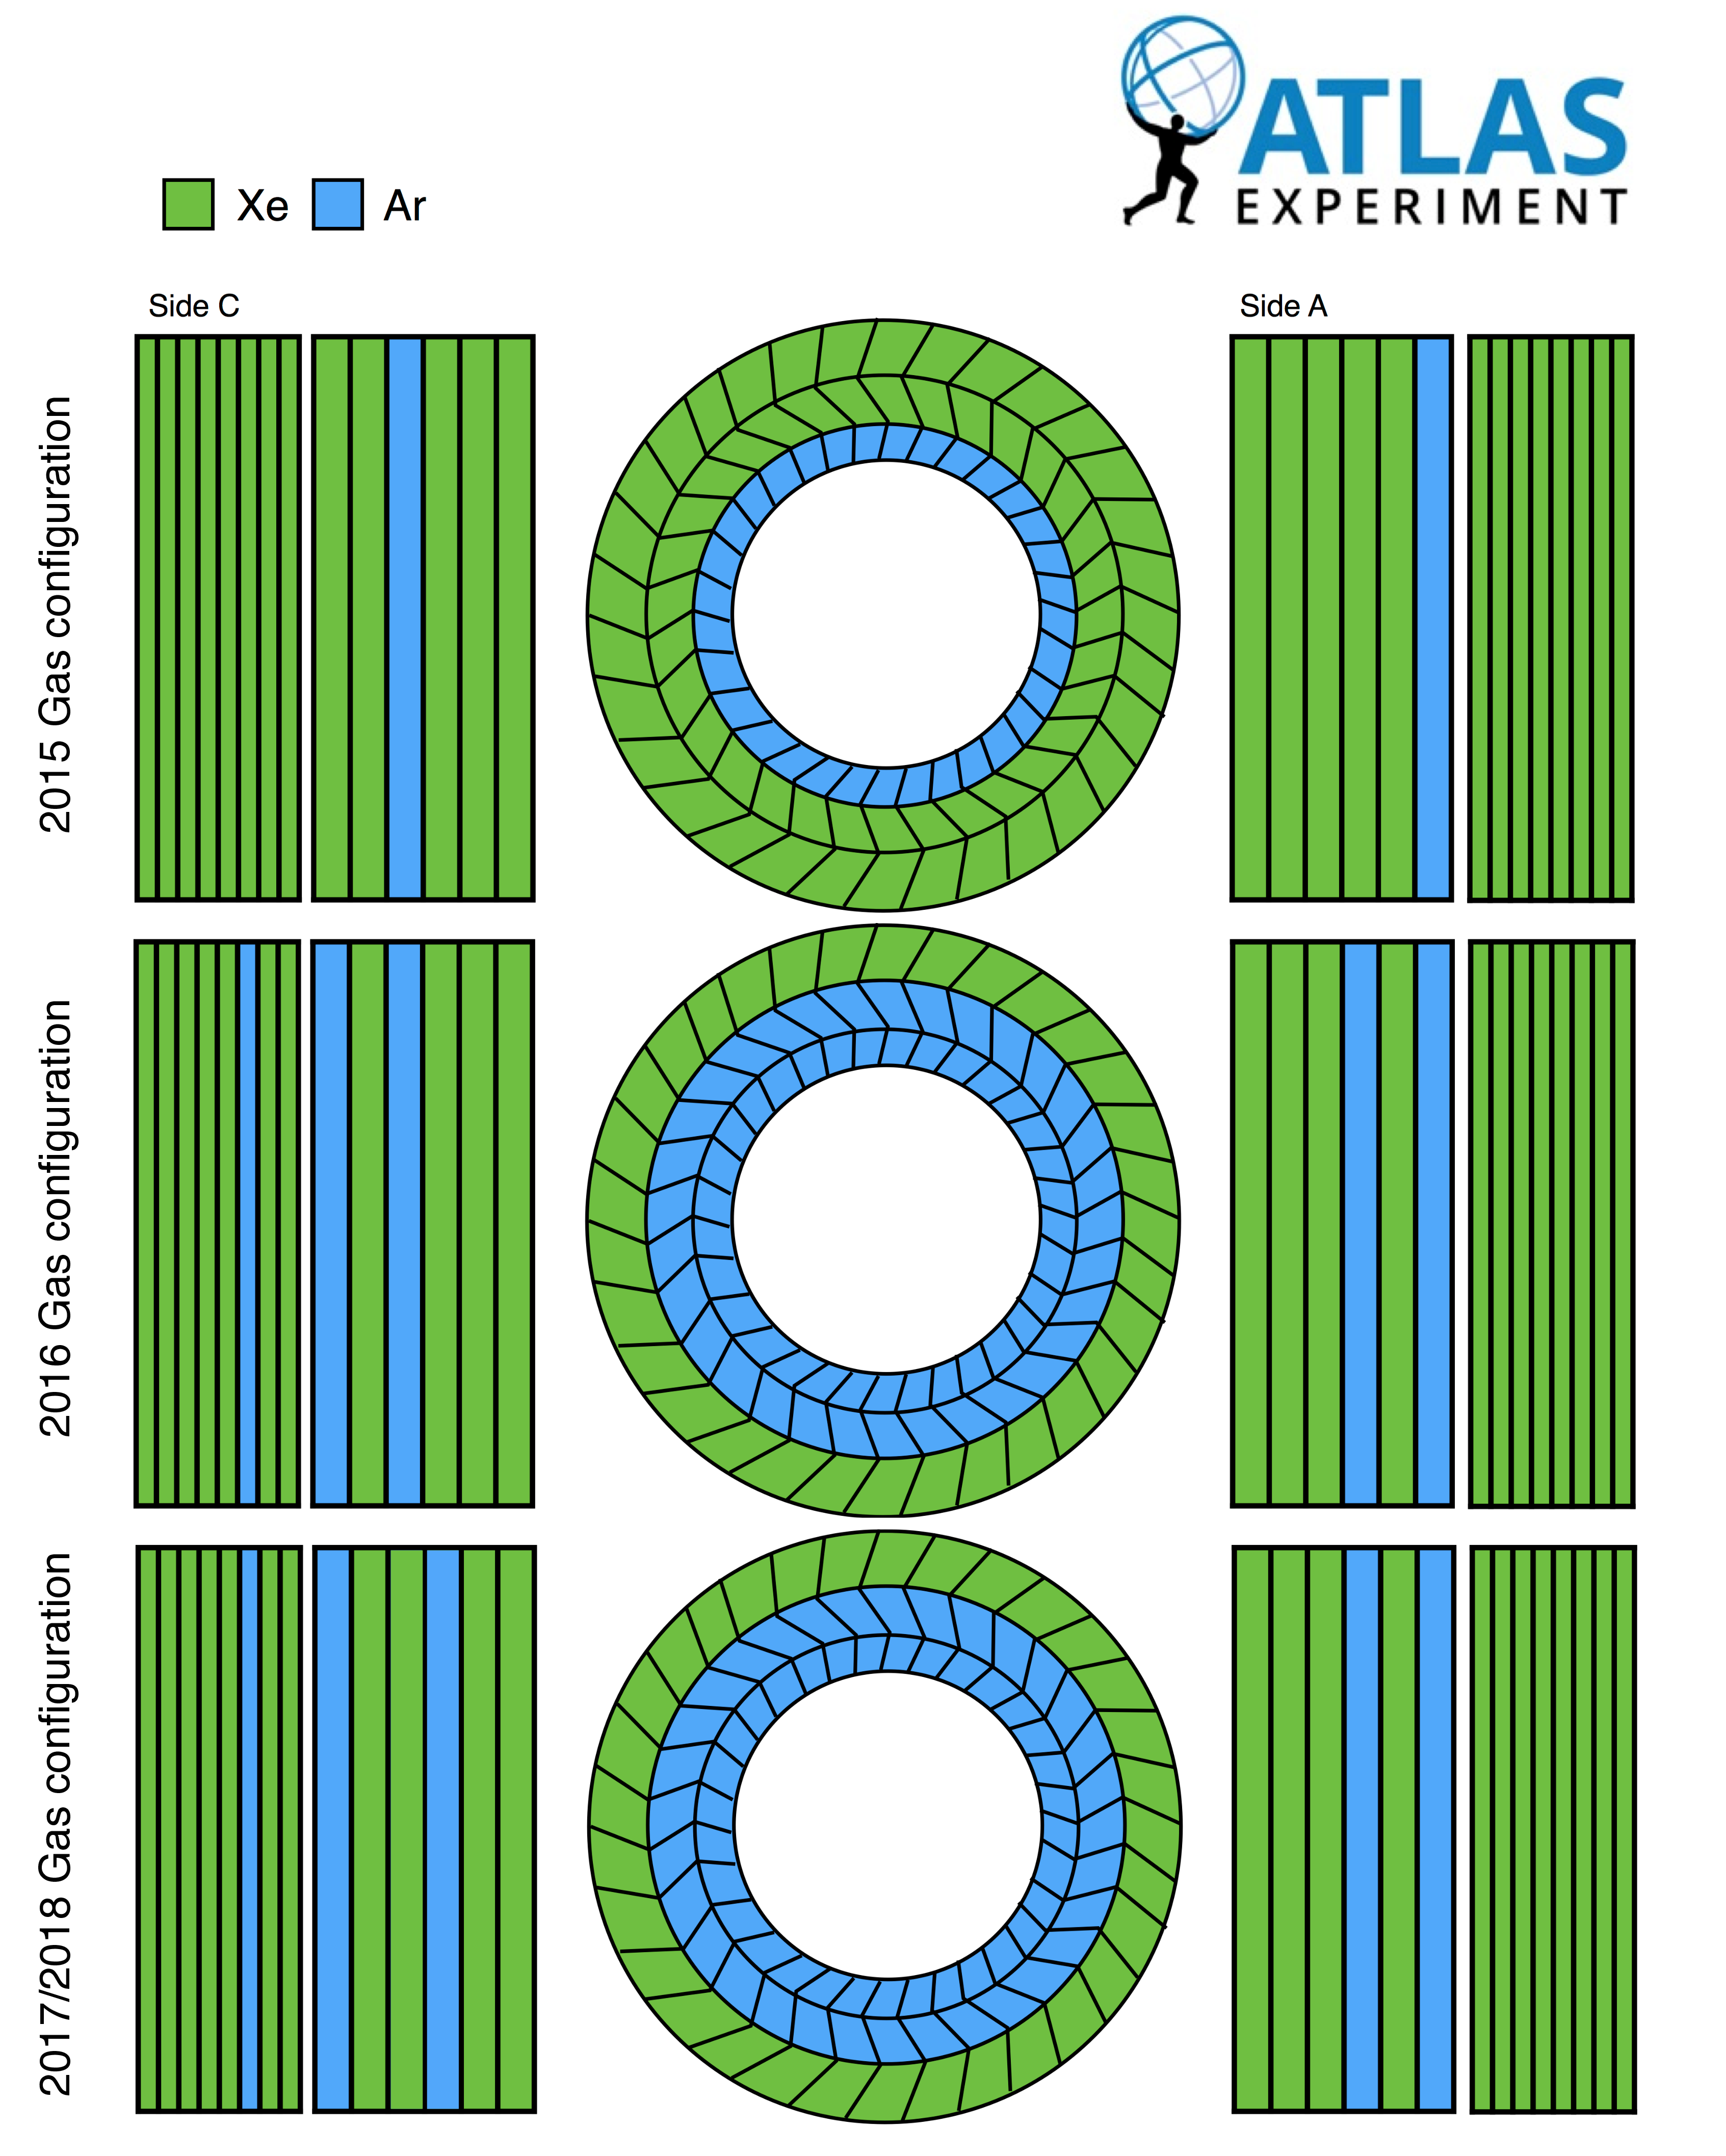
\includegraphics[width=0.80\textwidth]{figs/egamma/TRTGasConfig.png}
  %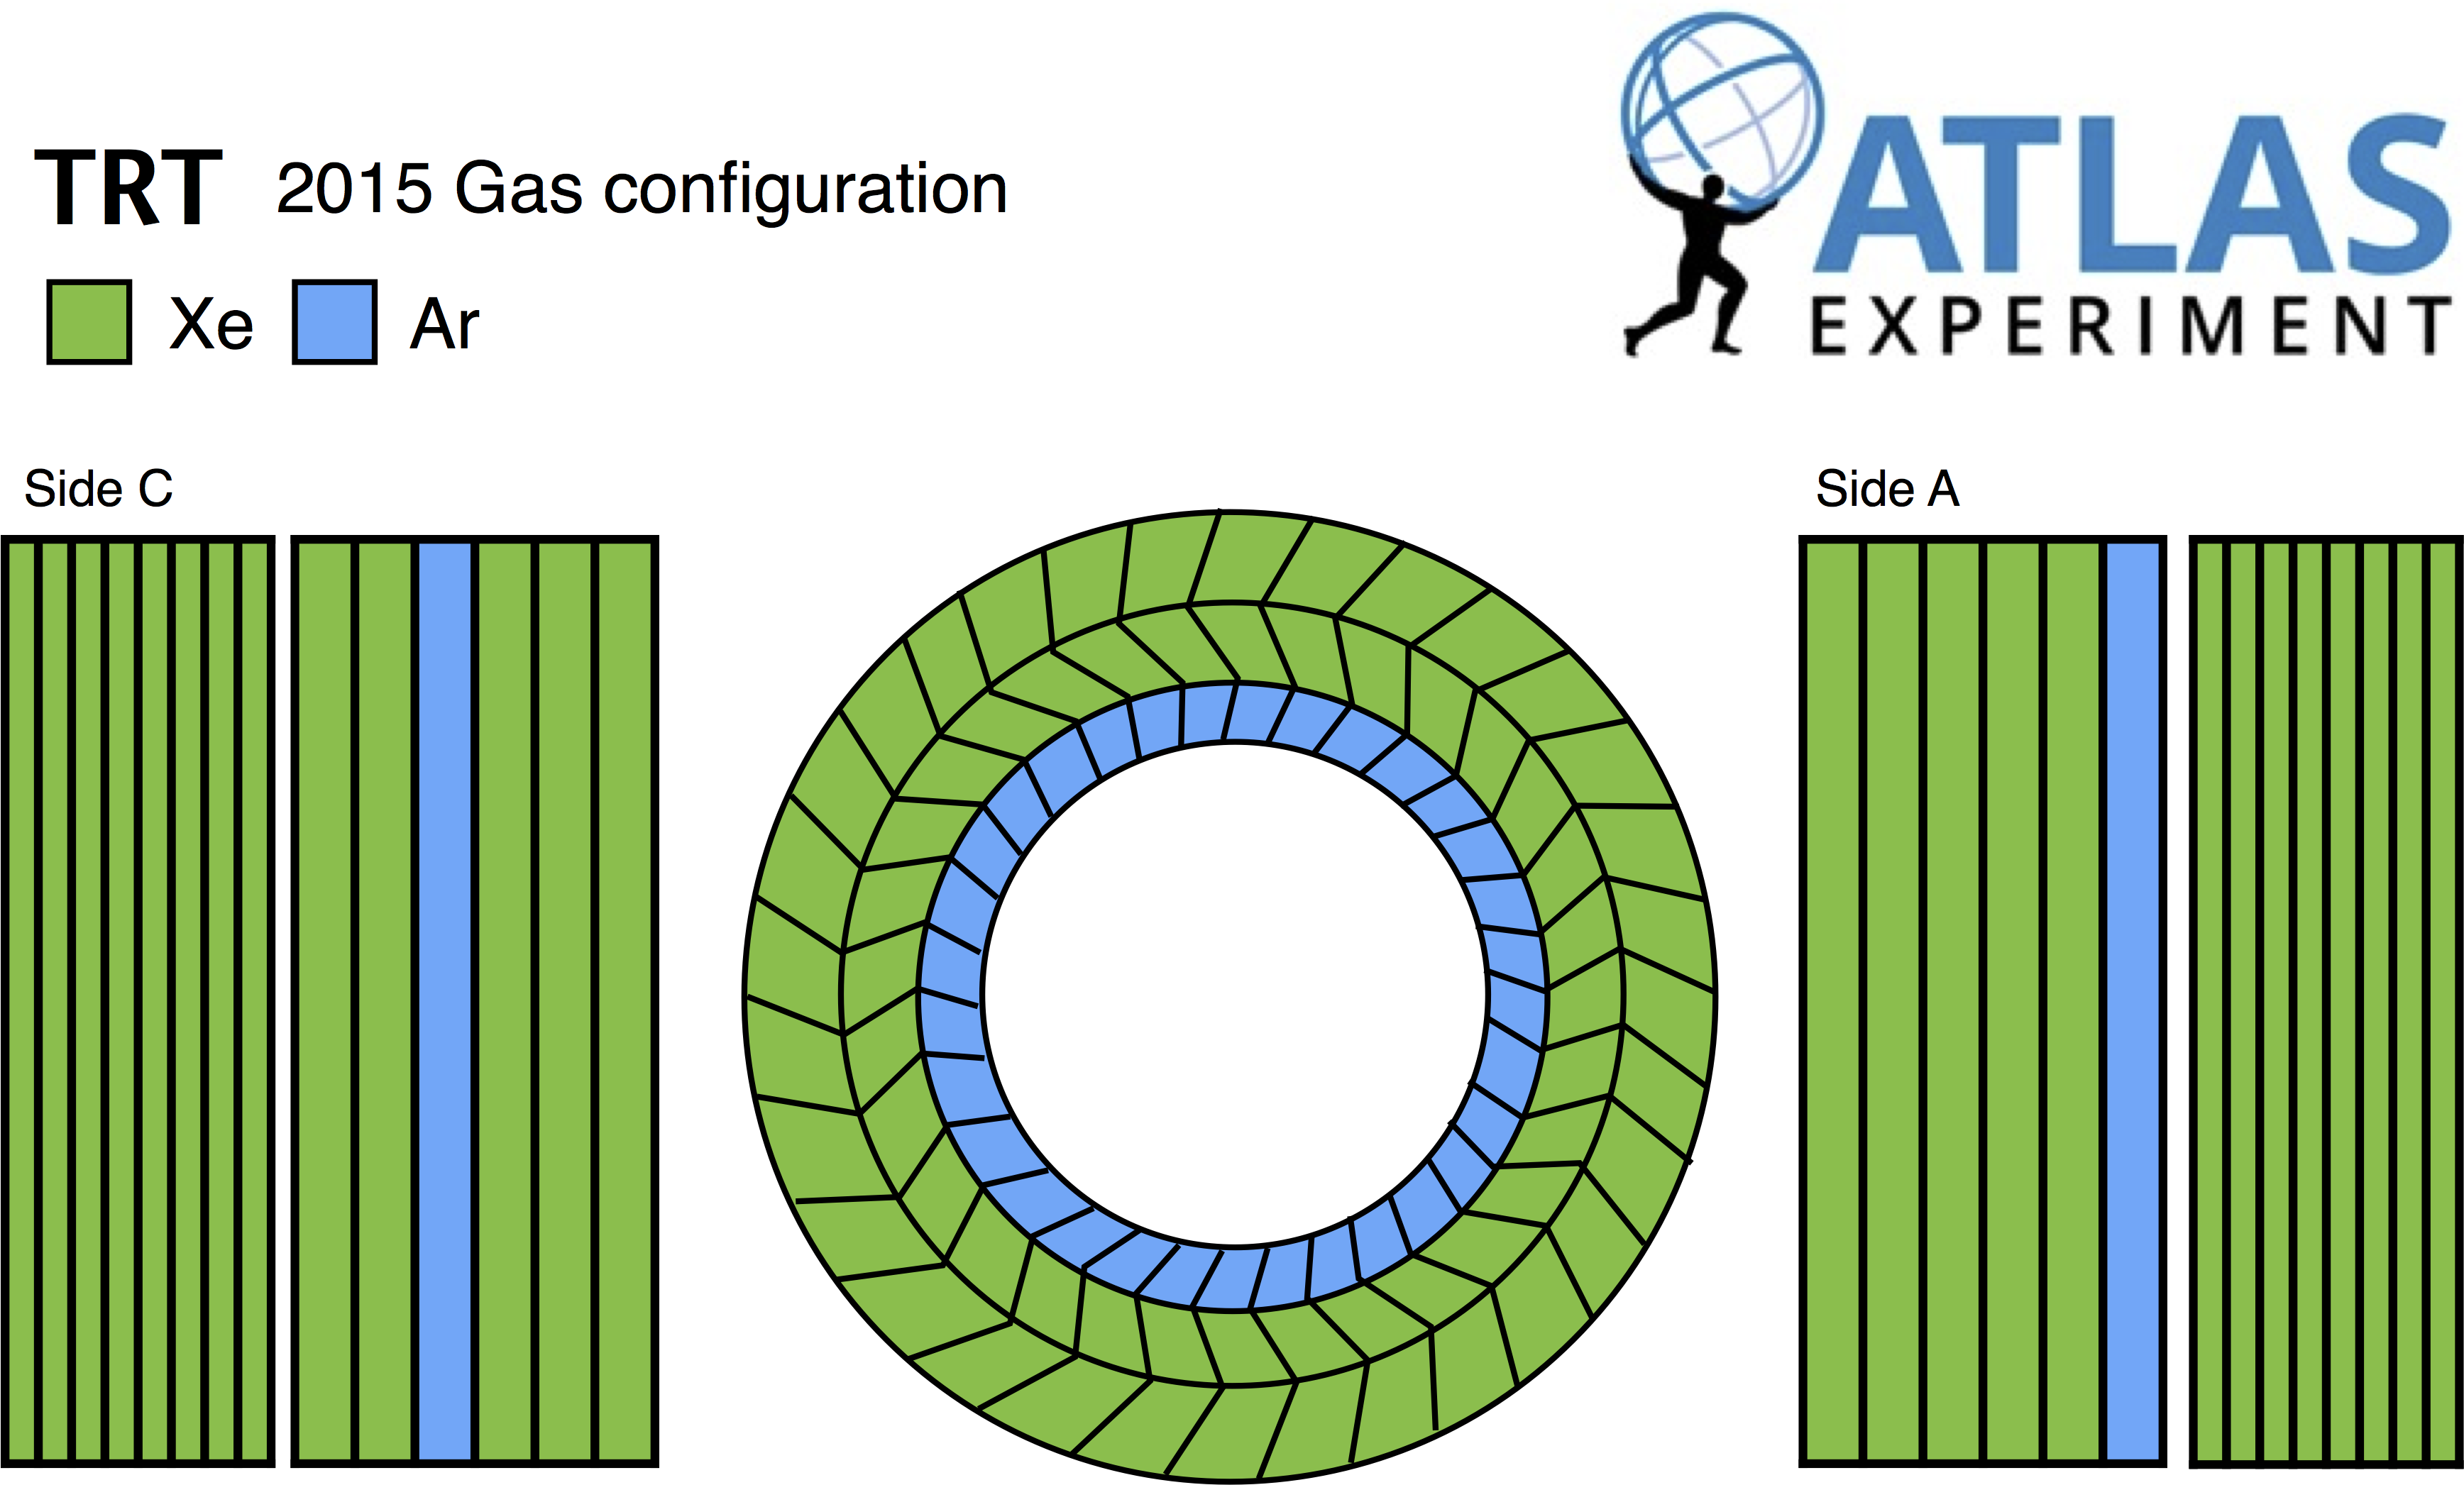
\includegraphics[width=0.90\textwidth]{figs/egamma/TRTGas2015-trim.png}
  %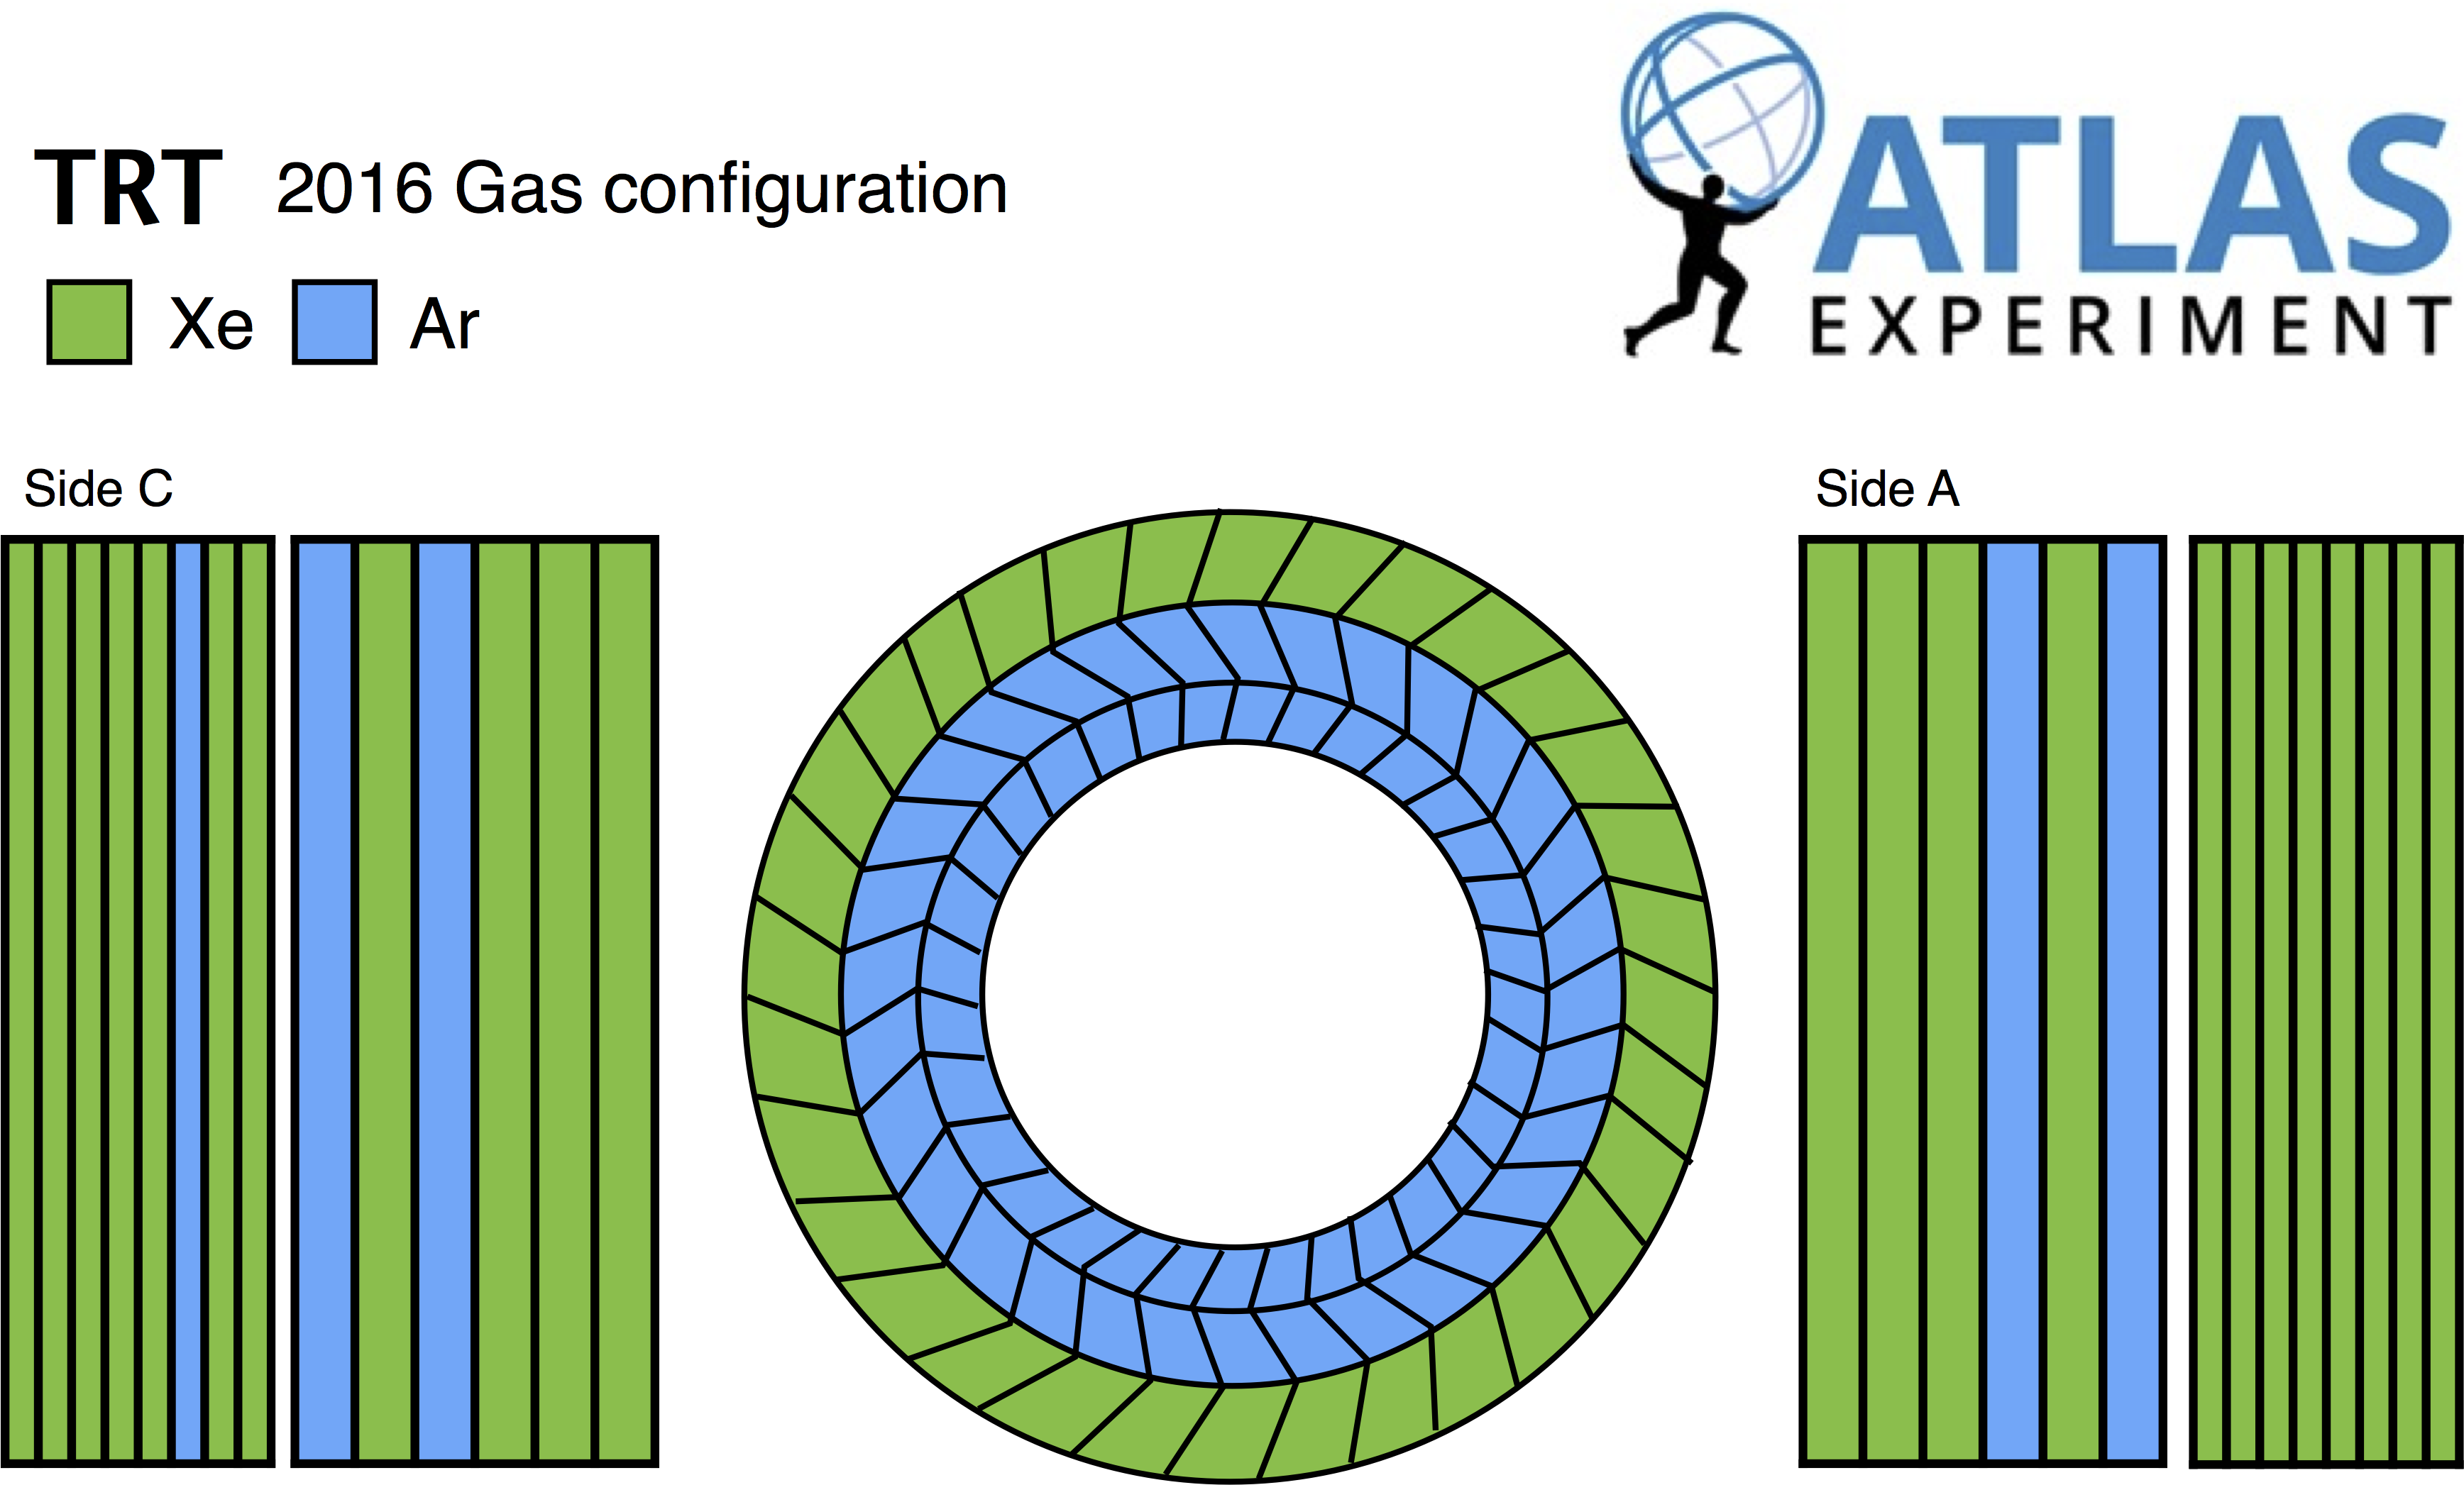
\includegraphics[width=0.90\textwidth]{figs/egamma/TRTGas2016-trim.png}
  % Optional first argument is what goes into the List of Figures, useful if main caption is long or contains references
  % Second argument here is the actual caption
  \caption[Cartoon illustrating the TRT gas configurations used in 2015 (top), 2016 (middle), and 2017/2018 (bottom).]{Cartoon illustrating the TRT gas configurations used in 2015 (top), 2016 (middle), and 2017/2018 (bottom). 
  Note that the concentric circles represent the TRT barrel layers while the rectangles represent each of the TRT endcap wheels \cite{TRTgas20152016}}
  \label{fig:egamma:TRTGas}
\end{figure}
%\subsection{The pdfs for the LH-identification}
%\label{sec:egamma:LHpdfs}
%Signal pdfs are built from either from MC or a relatively pure data sample of signal electrons.
%The goal is to build the signal pdfs from features that known electron, and not other object, signatures will have in the detectors.
%The signatures will vary depending on the energy of the electron and different paths it can take in the detector, and will therefore give us a distribution of values for a given discriminating variable obtained from a large training sample of electrons, effectively forming a pdf.
%This requires us to divide the likelihood, and therefore our pdfs, into the different $\et/\eta$ bins described in Section~\ref{sec:egamma:pdfbinning}.
%This is done for each variable in the suite of variables in Table \ref{tab:IDcuts} with an ``LH'' in it's last column.  


%building up feature rich distributions for the PDFs.  
%PDFs from electrons reconstructed in what most closely resembles the current detector geometry and conditions. 
%And so therein lies the argument to move from MC driven PDFs to data-driven PDFs, 
 %No one variable will uniquely discriminate your object from all other objects. A discriminating variable is a variable that is chosen on it merits of being able to discern an \emph{attribute} of the desired object from that attribute of as many other objects as possible. So then to actually use this to identify the desired object we naturally pick a collection of variables that provide good discriminating power for different object attributes for our desired object, building up a set of discriminating variables and their corresponding PDFs. At this point we are essentially done. The final step is to apply some smoothing to the PDFs to suppress unwanted statistical fluctuations that occur due to limited statistics and/or binning of the histogram. The method will be described in a later section. At this point we have our final set of PDFs that can be used by the likelihood.
 
\subsection{Constructing the pdfs}

During my time in the e/gamma group, I was one of the experts responsible for constructing the pdfs.
There were lots of changes during Run-2, from MC-based pdfs used for 2015-16, data-driven pdfs used in the trigger in 2017, and data-driven pdfs used in both the trigger and offline in 2018.
%With future reprocessing of Run-2 data, ?? data-driven pdfs will be used for offline for all years?
Many studies were required to check the performance of the electron identification.  I will describe here the derivation of the data-driven pdfs.
The signal pdfs are data-driven, using two samples.
%In Run-1, a data-driven selection was used to define the likelihood pdfs and discriminant cut values.
%For the likelihood used in Run-2, this was not possible at the initial startup (since the $\rts = 13\TeV$ data had not yet been collected), so MC-based pdfs were instead used.
%There have been several opportunities to update to $\rts = 13\TeV$ data-driven pdfs, but as the HLT likelihood was also MC-based through 2016, the decision was made to retain the MC-based pdfs offline as well, to reduce online-to-offline inefficiencies.
%For 2017, data-driven pdfs were derived for the trigger, and in 2018 the LH became fully data-driven when data-driven pdfs were derived for the offline LH as well.
Signal electrons with \pt\ $>$ 15~\GeV are selected using a \Zee \tnp selection. Events are collected using the primary single electron triggers.
The tag electrons must satisfy the \TightLH\ identification and have \pt\ $>$ 25~\GeV.
The selected probe electrons must form an invariant mass with the tag which falls within 10~\GeV of the \Zboson mass.
Additionally, the probes must satisfy the \VeryLooseLH\ identification, which is required in order to reduce fake lepton background contamination in the sample of probes, without significantly biasing the distributions of the discriminating variables.
Signal electrons with \pt\ $>$ 15~\GeV are selected using a \Jpsi\ \tnp selection. 
Events are collected using the secondary di-electron triggers.
As with the \Zee\ \tnp selection, tag electrons must satisfy the \TightLH\ identification, but are only required to have \pt\ $>$ 4.5~\GeV.
The probe electrons must form an invariant mass with the tag which falls within a 0.5 ~\GeV window of the \Jpsi\ mass and must satisfy the \VeryLooseLH\ identification.
Additionally, the tag and probe must be separated by $\Delta R > 0.1$ to avoid overlapping tag-probe pairs.
A cut is also placed on the pseudo-proper time:
\[\tau=\frac{L_{xy}\cdot m^{J/\psi}}{p_T^{J/\psi}}, \qquad \mathcal{L}_{xy}=\mathbf{L}\cdot\mathbf{p_T^{J/\psi}}/ p_T^{J/\psi}\]
in order to remove the non-prompt \Jpsi\ contribution coming from b-hadron decays~\cite{PERF-2016-01}.
These selections are summarized in Tables~\ref{tab:DataDrivenSignalSelection} and \ref{tab:DataDrivenJPsiSelection}.
\begin{table}[h]
\footnotesize
\renewcommand{\arraystretch}{1.16}
\begin{center}
  \begin{tabular}{l}
\textbf{Selection for data-driven signal electron candidates above 15~\GeV} \\
\hline
    Single electron trigger fired \\
    %see Table~\ref{tab:PrimaryTriggers} \\
    %Good Runs List \\                                                 
\midrule
    Tag electron with \pt\ $>$ 25~\GeV \\
    Tag electron $|\eta| < 1.37$ OR $(|\eta| > 1.52$ AND $|\eta| < 2.47)$ \\
    Tag electron passes \Tight\ identification \\
    $\Delta$R(tag electron, trigger electron) $<$ 0.10 \\
    Tag electron passes LAr object quality requirement \\
\midrule
    Probe electron with \pt\ $>$ 15~\GeV \\
    Probe electron $|\eta| < 2.47$ \\
    Probe electron passes \VeryLoose\ identification \\
    Probe electron passes LAr object quality requirement \\
\midrule
    80~\GeV $<$ \mee\ $<$ 100~\GeV \\
    Tag electron and probe electron have opposite electric charge \\
\hline
\end{tabular}
\end{center}
  \caption{Summary of data-driven signal electron selection above 15~\gev}
\label{tab:DataDrivenSignalSelection}
\end{table}
\begin{table}[h]
\footnotesize
\renewcommand{\arraystretch}{1.16}
\begin{center}
  \begin{tabular}{l}
\textbf{Selection for data-driven signal electron candidates below 15~\GeV} \\
\hline
    Di-electron trigger fired \\
    %see Table~\ref{tab:JpsiTriggers} \\
    %Good Runs List \\ 
\midrule
    Tag electron with \pt\ $>$ 4.5~\GeV \\
    Tag electron $|\eta| < 1.37$ OR $(|\eta| > 1.52$ AND $|\eta| < 2.47)$ \\
    Tag electron passes \Tight\ identification \\
    $\Delta$R(tag electron, trigger electron) $<$ 0.10 \\
    Tag electron passes LAr object quality requirement \\
\midrule
    Probe electron with \pt\ $>$ 4.5~\GeV \\
    Probe electron $|\eta| < 2.47$ \\
    Probe electron passes \VeryLoose\ identification \\
    Probe electron passes LAr object quality requirement \\
\midrule
    2.8~\GeV $<$ \mee $<$ 3.3~\GeV \\
    Tag electron and probe electron have opposite electric charge \\
    $\Delta$R(tag electron, probe electron) $>$ 0.10 \\
    $-1 < \tau < 0.2$\\
\hline
\end{tabular}
\end{center}
  \caption{Summary of data-driven signal electron selection below 15~\gev}
\label{tab:DataDrivenJPsiSelection}
\end{table}

Background events are collected using the prescaled single electron support triggers.
These triggers require an electron to pass a \pt\ threshold, but do not apply any identification requirement at the HLT.
Note that jets are frequently also reconstructed as electrons, due to the requirements imposed on the tracking hits and calorimeter energy deposition during the reconstruction stage.
Thus, this sample primarily contains dijet events, which is the process with the largest production cross-section at the LHC.
However, this is a very inclusive selection, and thus includes other processes as well.
To reduce potential contamination from electroweak processes containing real, prompt electrons, the following requirements are applied:
\begin{itemize}
\item{If \MET\ $>$ 25~\GeV, veto the event (reduce contamination from \Wenu\ decays)}
\item{If \mT\ $>$ 40~\GeV, veto the event (reduce contamination from \Wenu\ decays)}
\item{If a second electron (which passes \Medium\ and has \pt $>$ 4~\GeV) exists 
  in the event and forms an invariant mass within 70~\GeV $<$ \mee\ $<$ 110~\GeV, 
    veto the event (reduce contamination from \Zee\ decays). 
    Note that no charge requirements are placed on these electrons, 
    to suppress the (admittedly small) contamination from charge-flip \Zee electrons}
\end{itemize}
These selections are summarized in Table~\ref{tab:DataDrivenBackgroundSelection}.
\begin{table}[h]
\footnotesize
\renewcommand{\arraystretch}{1.26}
\begin{center}
  \begin{tabular}{l}
\textbf{Selection for data-driven background electron candidates} \\
\hline
    Prescaled single electron supporting trigger fired\\
    %see Table~\ref{tab:SupportTriggers} \\
\midrule
    Electron candidate with \pt\ $>$ 4~\GeV \\
    Electron candidate $|\eta| < 2.47$ \\
    Electron candiate has good track-quality ($n_{\mathrm{Pixel}} \geq 1$, $n_{\mathrm{Silicon}} \geq 7$) \\
    $\Delta$R(reco electron candidate, trigger electron) $<$ 0.10 \\
    Electron candidate passes LAr object quality requirement \\
\midrule
    \MET $<$ 25~\GeV \\
    \mT $<$ 40~\GeV \\
    (70~\GeV $<$ \mee\ $||$ \mee\ $>$ 110~\GeV) for events containing an additional \Medium\ electron \\
\hline
\end{tabular}
\end{center}
  \caption[Summary of data-driven background electron selection]{Summary of data-driven background electron selection}
\label{tab:DataDrivenBackgroundSelection}
\end{table}

%\begin{table}
%\footnotesize
%\renewcommand{\arraystretch}{1.3}
%\begin{center}
%  \begin{tabular}{l}
%\textbf{Primary single electron triggers} \\
%\hline
%HLT\_e26\_lhtight\_nod0\_ivarloose \\
%HLT\_e60\_lhmedium\_nod0 \\
%HLT\_e140\_lhloose\_nod0 \\
%HLT\_e300\_etcut \\
%\hline
%\end{tabular}
%\end{center}
%  \caption{List of primary electron triggers (unprescaled) in 2016}
%\label{tab:PrimaryTriggers}
%\end{table}

%\begin{table}
%\footnotesize
%\renewcommand{\arraystretch}{1.3}
%\begin{center}
%  \begin{tabular}{l}
%\hline
%\textbf{Prescaled \Jpsi supporting di-electron triggers}\\
%HLT\_e5\_lhtight\_nod0\_e4\_etcut\_Jpsiee \\
%HLT\_e9\_lhtight\_nod0\_e4\_etcut\_Jpsiee \\
%HLT\_e14\_lhtight\_nod0\_e4\_etcut\_Jpsiee \\
%HLT\_e9\_etcut\_e5\_lhtight\_nod0\_Jpsiee \\
%HLT\_e14\_etcut\_e5\_lhtight\_nod0\_Jpsiee \\
%\hline
%\end{tabular}
%\end{center}
%  \caption{List of \Jpsi supporting di-electron triggers (prescaled) in 2016}
%\label{tab:JpsiTriggers}
%\end{table}

%\begin{table}
%\footnotesize
%\renewcommand{\arraystretch}{1.3}
%\begin{center}
%  \begin{tabular}{l}
%\textbf{Prescaled single electron supporting triggers} \\
%\hline
%    HLT\_e5\_etcut \\
%    HLT\_e10\_etcut\_L1EM7 \\
%    HLT\_e15\_etcut\_L1EM7 \\
%    HLT\_e20\_etcut\_L1EM12 \\
%    HLT\_e25\_etcut\_L1EM15 \\
%    HLT\_e30\_etcut\_L1EM15 \\
%    HLT\_e40\_etcut\_L1EM15 \\
%    HLT\_e50\_etcut\_L1EM15 \\
%    HLT\_e60\_etcut \\
%    HLT\_e70\_etcut \\
%    HLT\_e80\_etcut \\
%    HLT\_e100\_etcut \\
%    HLT\_e120\_etcut \\
%\hline
%\end{tabular}
%\end{center}
%  \caption{List of prescaled single electron supporting triggers in 2016}
%\label{tab:SupportTriggers}
%\end{table}

\subsubsection{Binning in $E_{\mathrm{T}}$ and \(\eta\)}
\label{sec:egamma:pdfbinning}
The shape of the discriminating variable distributions vary according to the detector geometry, whose features in $\eta$ are dictated by the cylindrical nature of its barrel subdetectors, the transition to endcap detectors, the space dedicated to structure and services, and the amount of material before the calorimeters.
The identification is split in $\eta$ to account for these variations such that the discriminant variables have negligible variation within an $\eta$ slice (for a constant \et).
The bin thresholds chosen are shown in Table \ref{tab:etabins} below and graphically depicted in Figure \ref{fig:egamma:LHetaBinning} where these geometry and material transitions can be seen explicitly.
Variable distributions also vary as a function of object \et; thus, the phase space is split further into \et\ bins, typically in 5 GeV increments.
The \et\ bin thresholds used are shown in Tables~\ref{tab:etbins}.
To avoid large discontinuities near \et\ bin edges when using a finer granularity than what is shown in Table~\ref{tab:etbins}, a linear interpolation between neighboring \et\ bins is used to extract an interpolated pdf value as well as an interpolated discriminant cut value.
\begin{table*}[h]
\begin{center}
  \begin{tabular}{cccccccccc}
\hline
\multicolumn{10}{c}{Bin boundaries in $|\eta|$}\\
\hline
0.0& 0.6& 0.8& 1.15& 1.37& 1.52& 1.81& 2.01& 2.37& 2.47 \\
\hline
\end{tabular}
\end{center}
\caption[Boundaries in absolute cluster pseudorapidity used to define the nine bins for the LH pdfs and LH discriminant requirements.]{Boundaries in absolute cluster pseudorapidity used to define the nine bins for the LH pdfs and LH discriminant requirements.}
\label{tab:etabins}
\end{table*}
\begin{table*}[h]
\begin{center}
\begin{tabular}{l|ccccccccccccc}
\hline
\multicolumn{14}{c}{Bin boundaries in \Et\ [\GeV]}\\
\hline
pdfs         & 4.5& 7& 10& 15& 20&   & 30&   & 40&   &   &    & $\infty$ \\
Discriminant & 4.5& 7& 10& 15& 20& 25& 30& 35& 40& 45& 80& 150& $\infty$ \\
\hline
\end{tabular}
\end{center}
\caption[Boundaries in electron transverse energy used to define the seven bins for the LH pdfs and the twelve bins for LH discriminant requirements.]{Boundaries in electron transverse energy used to define the seven bins for the LH pdfs and the twelve bins for LH discriminant requirements.}
%  The twelve bins in the table correspond to the data accumulated in 2016.
%  For the 2015 data the bin boundaries at 80~\GeV\ and 150~\GeV\ were 100~\GeV\ and 125~\GeV.
%}
\label{tab:etbins}
\end{table*}
\begin{figure}[h]
  \centering
  %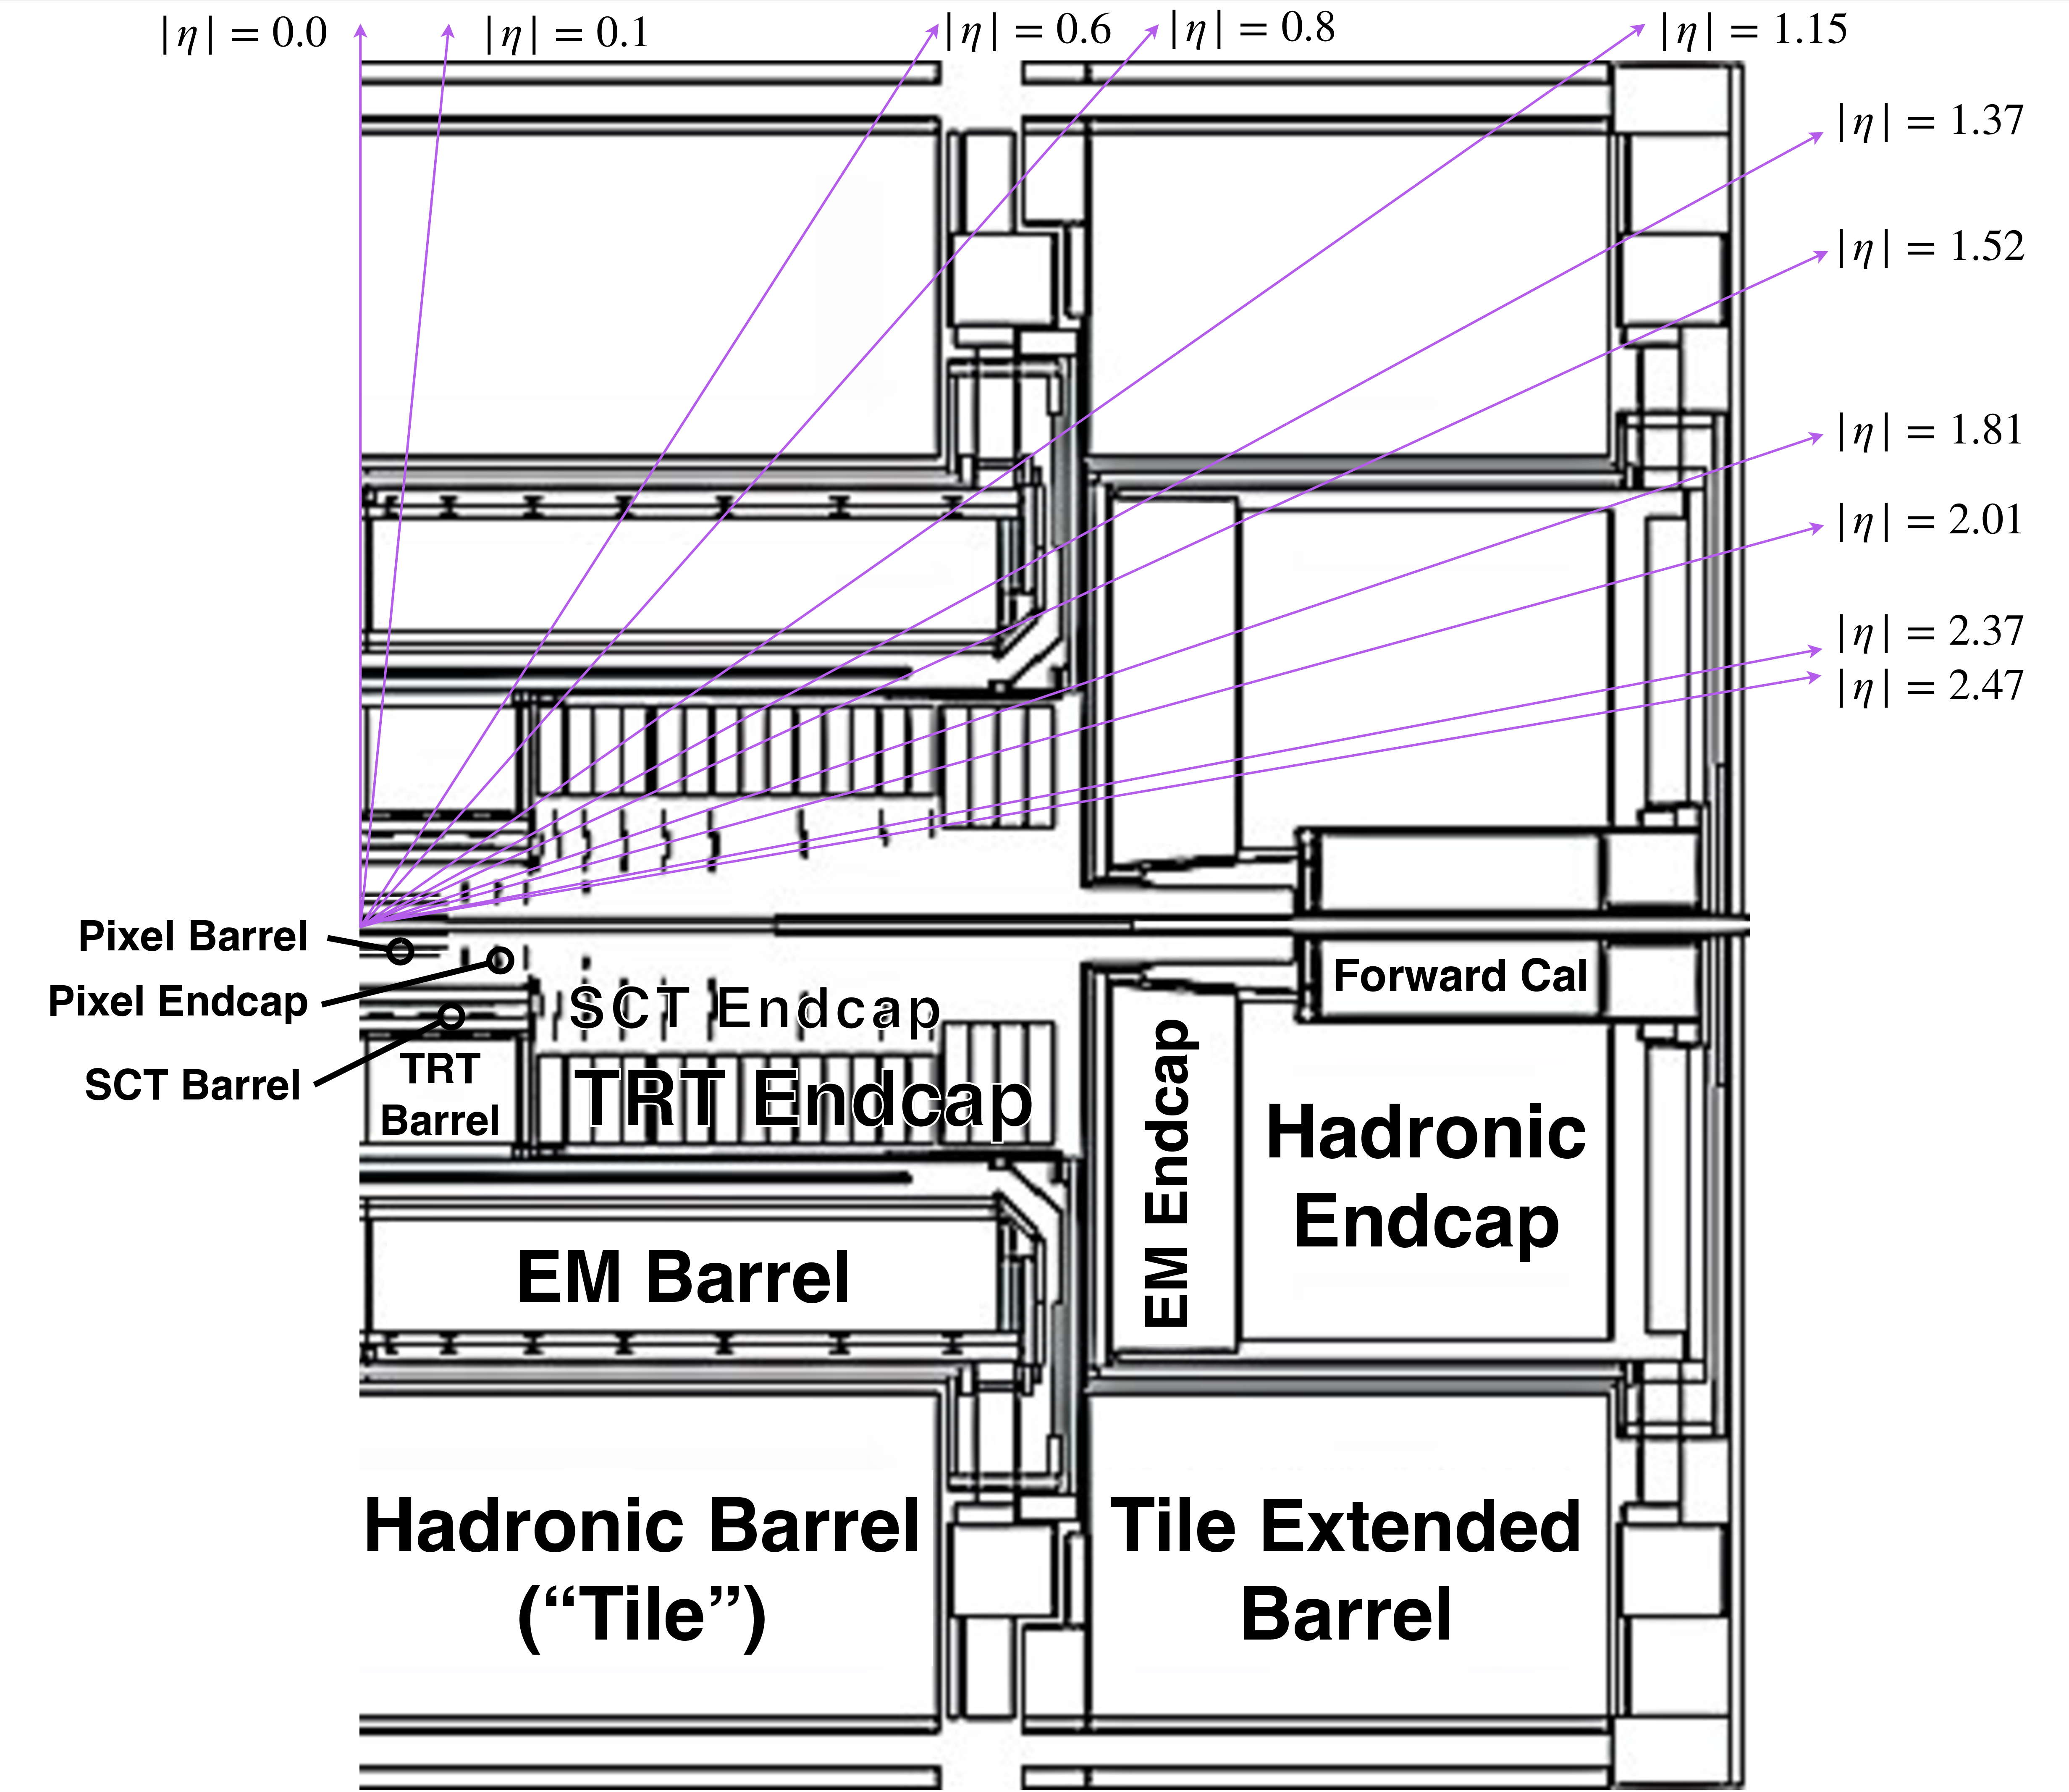
\includegraphics[width=1.0\textwidth]{figs/egamma/LHpdfEtaBinning.pdf}
  \makebox[\textwidth][c]{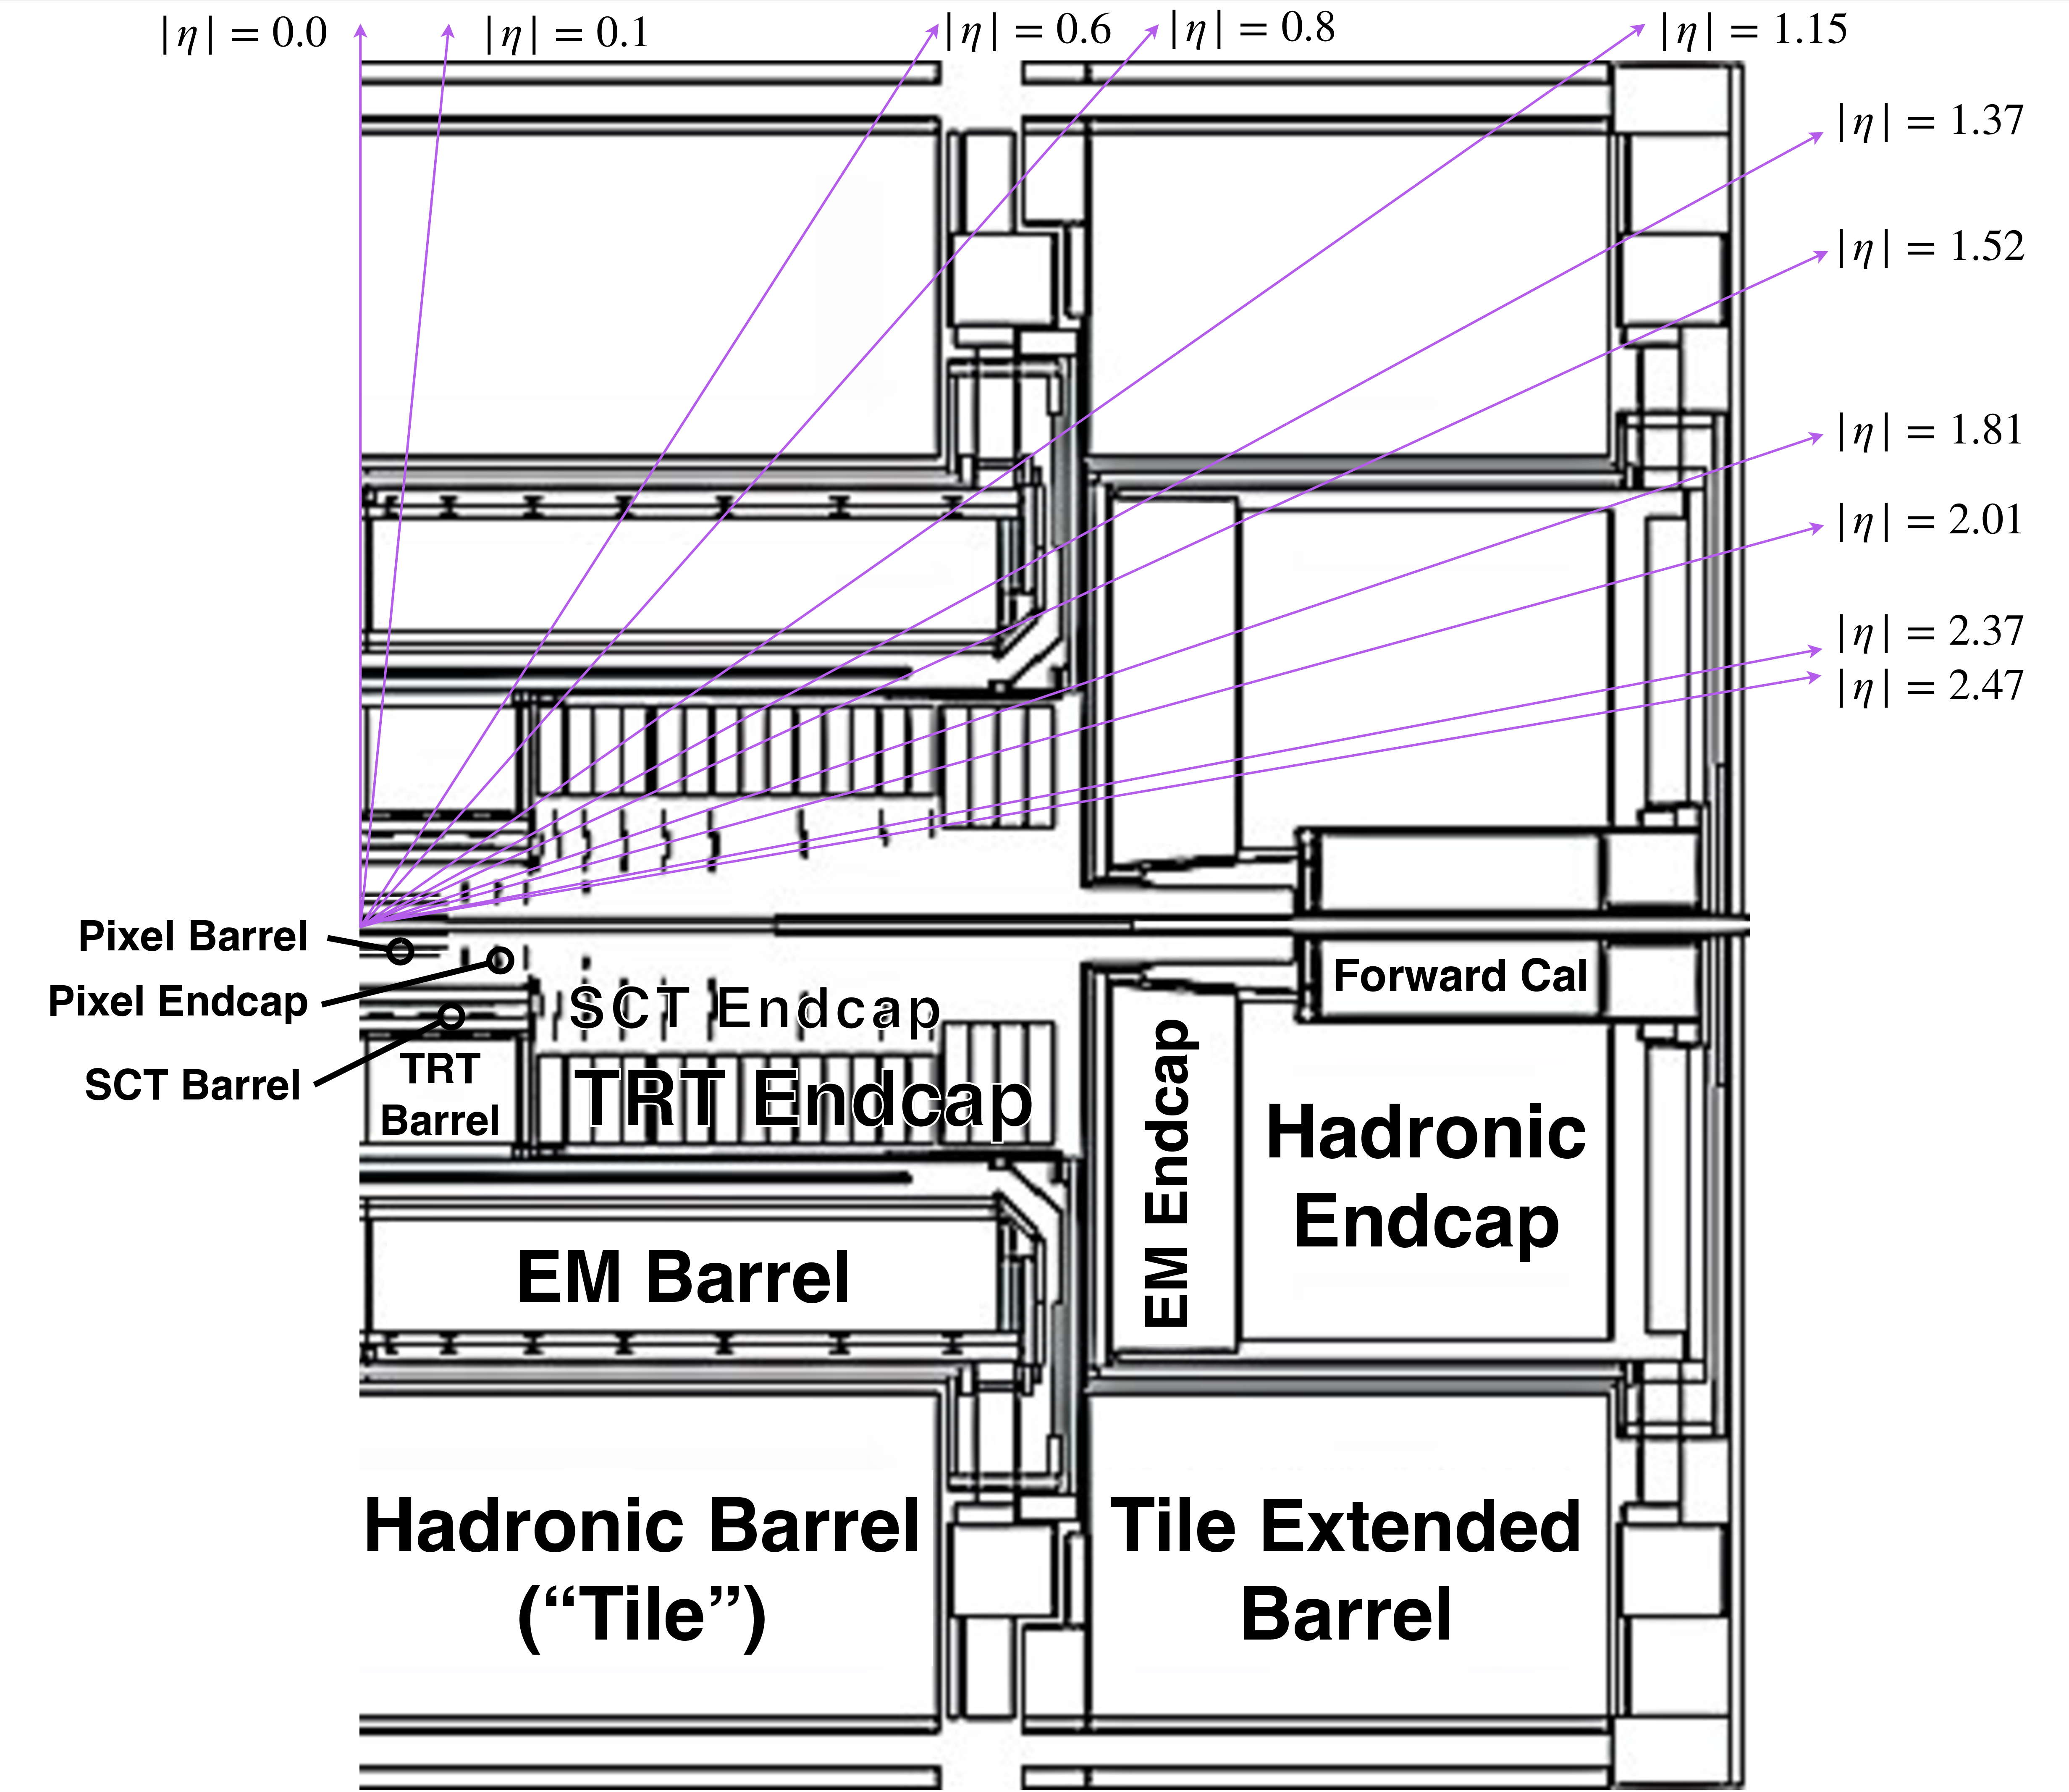
\includegraphics[width=1.2\textwidth]{figs/egamma/LHpdfEtaBinning.png}}
  \caption[Cartoon of the middle cross-section of one side of the calorimeters and ID showing the $\eta$ regions the LH is binned in.]
          {Cartoon of the middle cross-section of one side of the calorimeters and ID showing the $\eta$ regions the LH is binned in.}
  \label{fig:egamma:LHetaBinning}
\end{figure}


\subsubsection{Smoothing: Adaptive Kernel Density Estimation (KDE)}
%The pdfs are created from finely binned histograms of the individual discriminating variables. 
%To avoid non-physical fluctuations in the pdfs arising from the limited statistics of the simulations samples, the histograms are smoothed using an adaptive kernel density estimation (KDE) implemented in the TMVA toolkit~\cite{Hocker:2007ht}.
To first approximation, pdfs can be obtained by simply building a histogram of each variable using the signal and background samples as described in the previous section. However, logistical issues of bin granularity and limited statistics could adversely affect the performance of the likelihood. 
The electron likelihood should be constructed from pdfs containing only meaningful physical features.
Random statistical fluctuations, particularly in the pdfs of likelihoods covering regions of $\eta$/\et\ where signal or background statistics are low, can cause suboptimal behavior, such as nearly identical electrons being assigned vastly different discriminant values.
Likewise, the pdfs should be nonzero everywhere, to avoid undefined or unphysical results. Thus, raw histogram pdfs must be transformed to solve these issues.
Adaptive kernel density estimation (KDE) is used to convert the histogrammed signal and background samples into pdf inputs for the likelihood.
The KDE method smooths a variable distribution in the following manner: first, the value in each bin in the variable’s distribution is treated as a  $\delta$-function. 
Each $\delta$ function then replaced by a ``kernel'' function (in this case a Gaussian distribution) with a tunable width parameter, and the collection of Gaussian distributions are summed to form the final pdf.
The adaptive KDE method follows the same procedure, but the Gaussian width parameter is increased in regions of low event yields as is illustrated in Figure~\ref{fig:egamma:AKDE}) \cite{Hocker}.
The pdfs developed for the electron likelihood tool were created using the TMVA adaptive KDE tool.
In practice, the tool uses very finely binned histograms to approximate the $\delta$ functions of an unbinned dataset, in order to increase the algorithm speed, without loss of performance.
Figure \ref{fig:egamma:KDEexample} illustrates the adaptive KDE method at work in an example \reta\ distribution where we see nonphysical features being smoothed out by the method.
\begin{figure}[h]
\centering
    \begin{subfigure}[b]{0.49\textwidth}
      \centering
      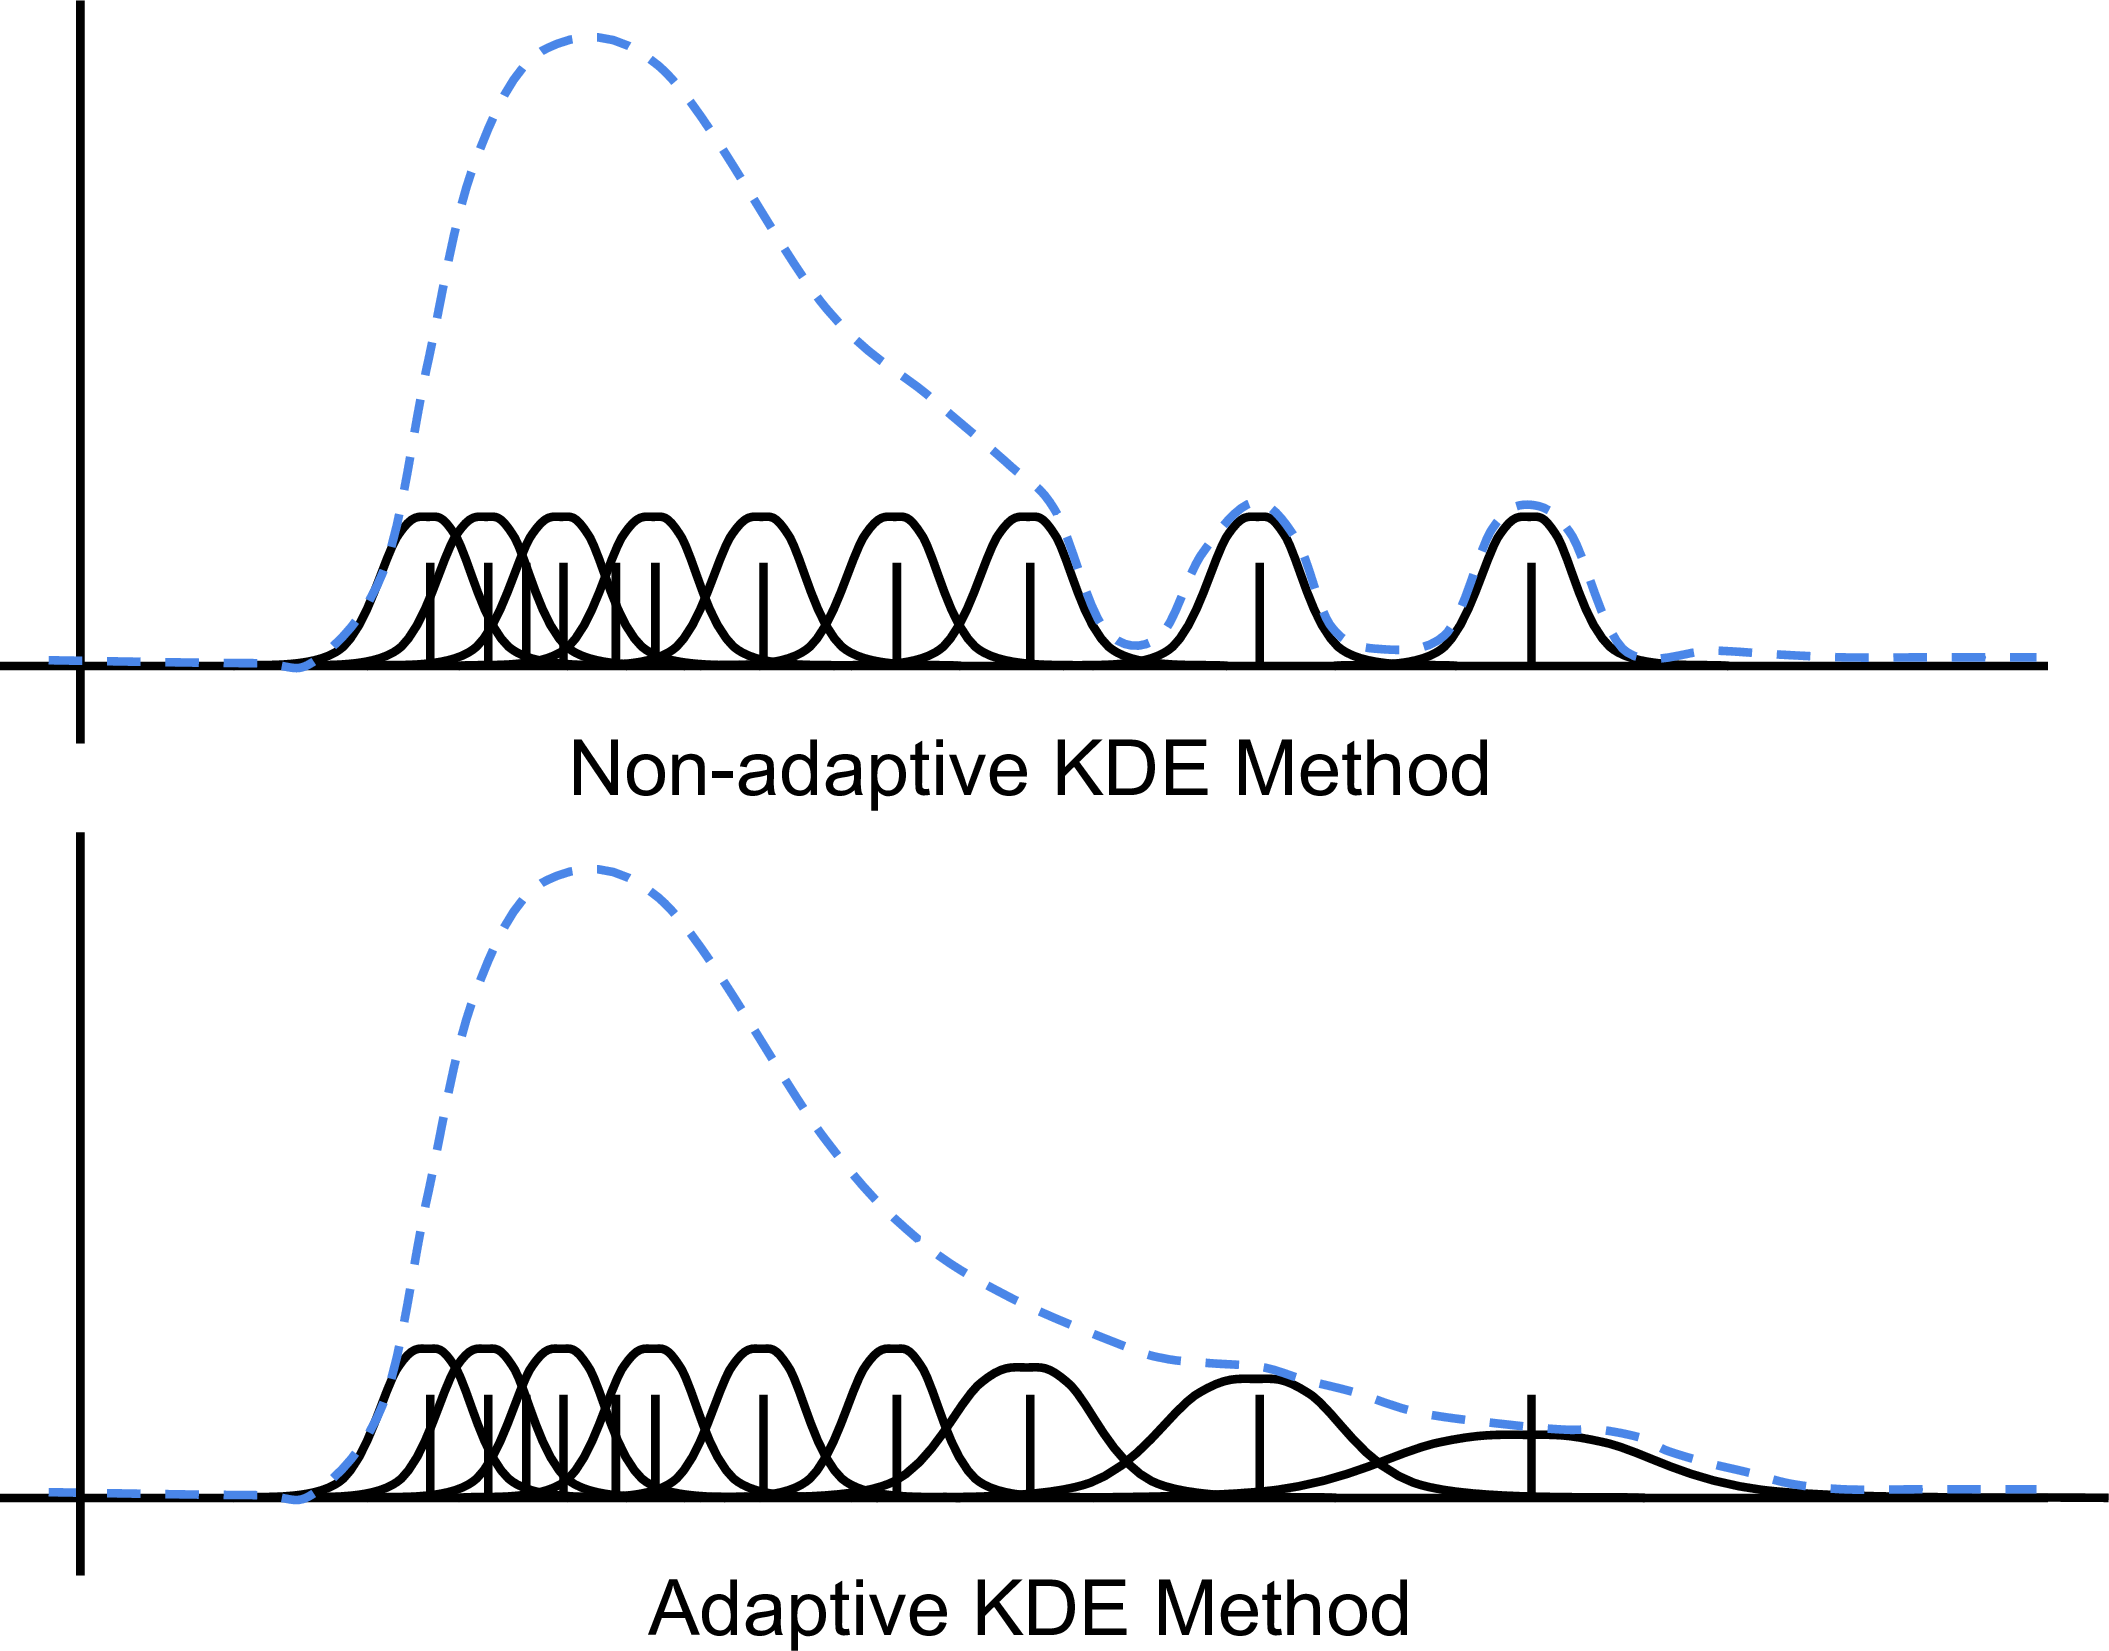
\includegraphics[width=.98\textwidth]{figs/egamma/KDEMethod.png}
      \caption{}
      \label{fig:egamma:AKDE}
    \end{subfigure}
    \hfill
    \begin{subfigure}[b]{0.49\textwidth}
      \centering
      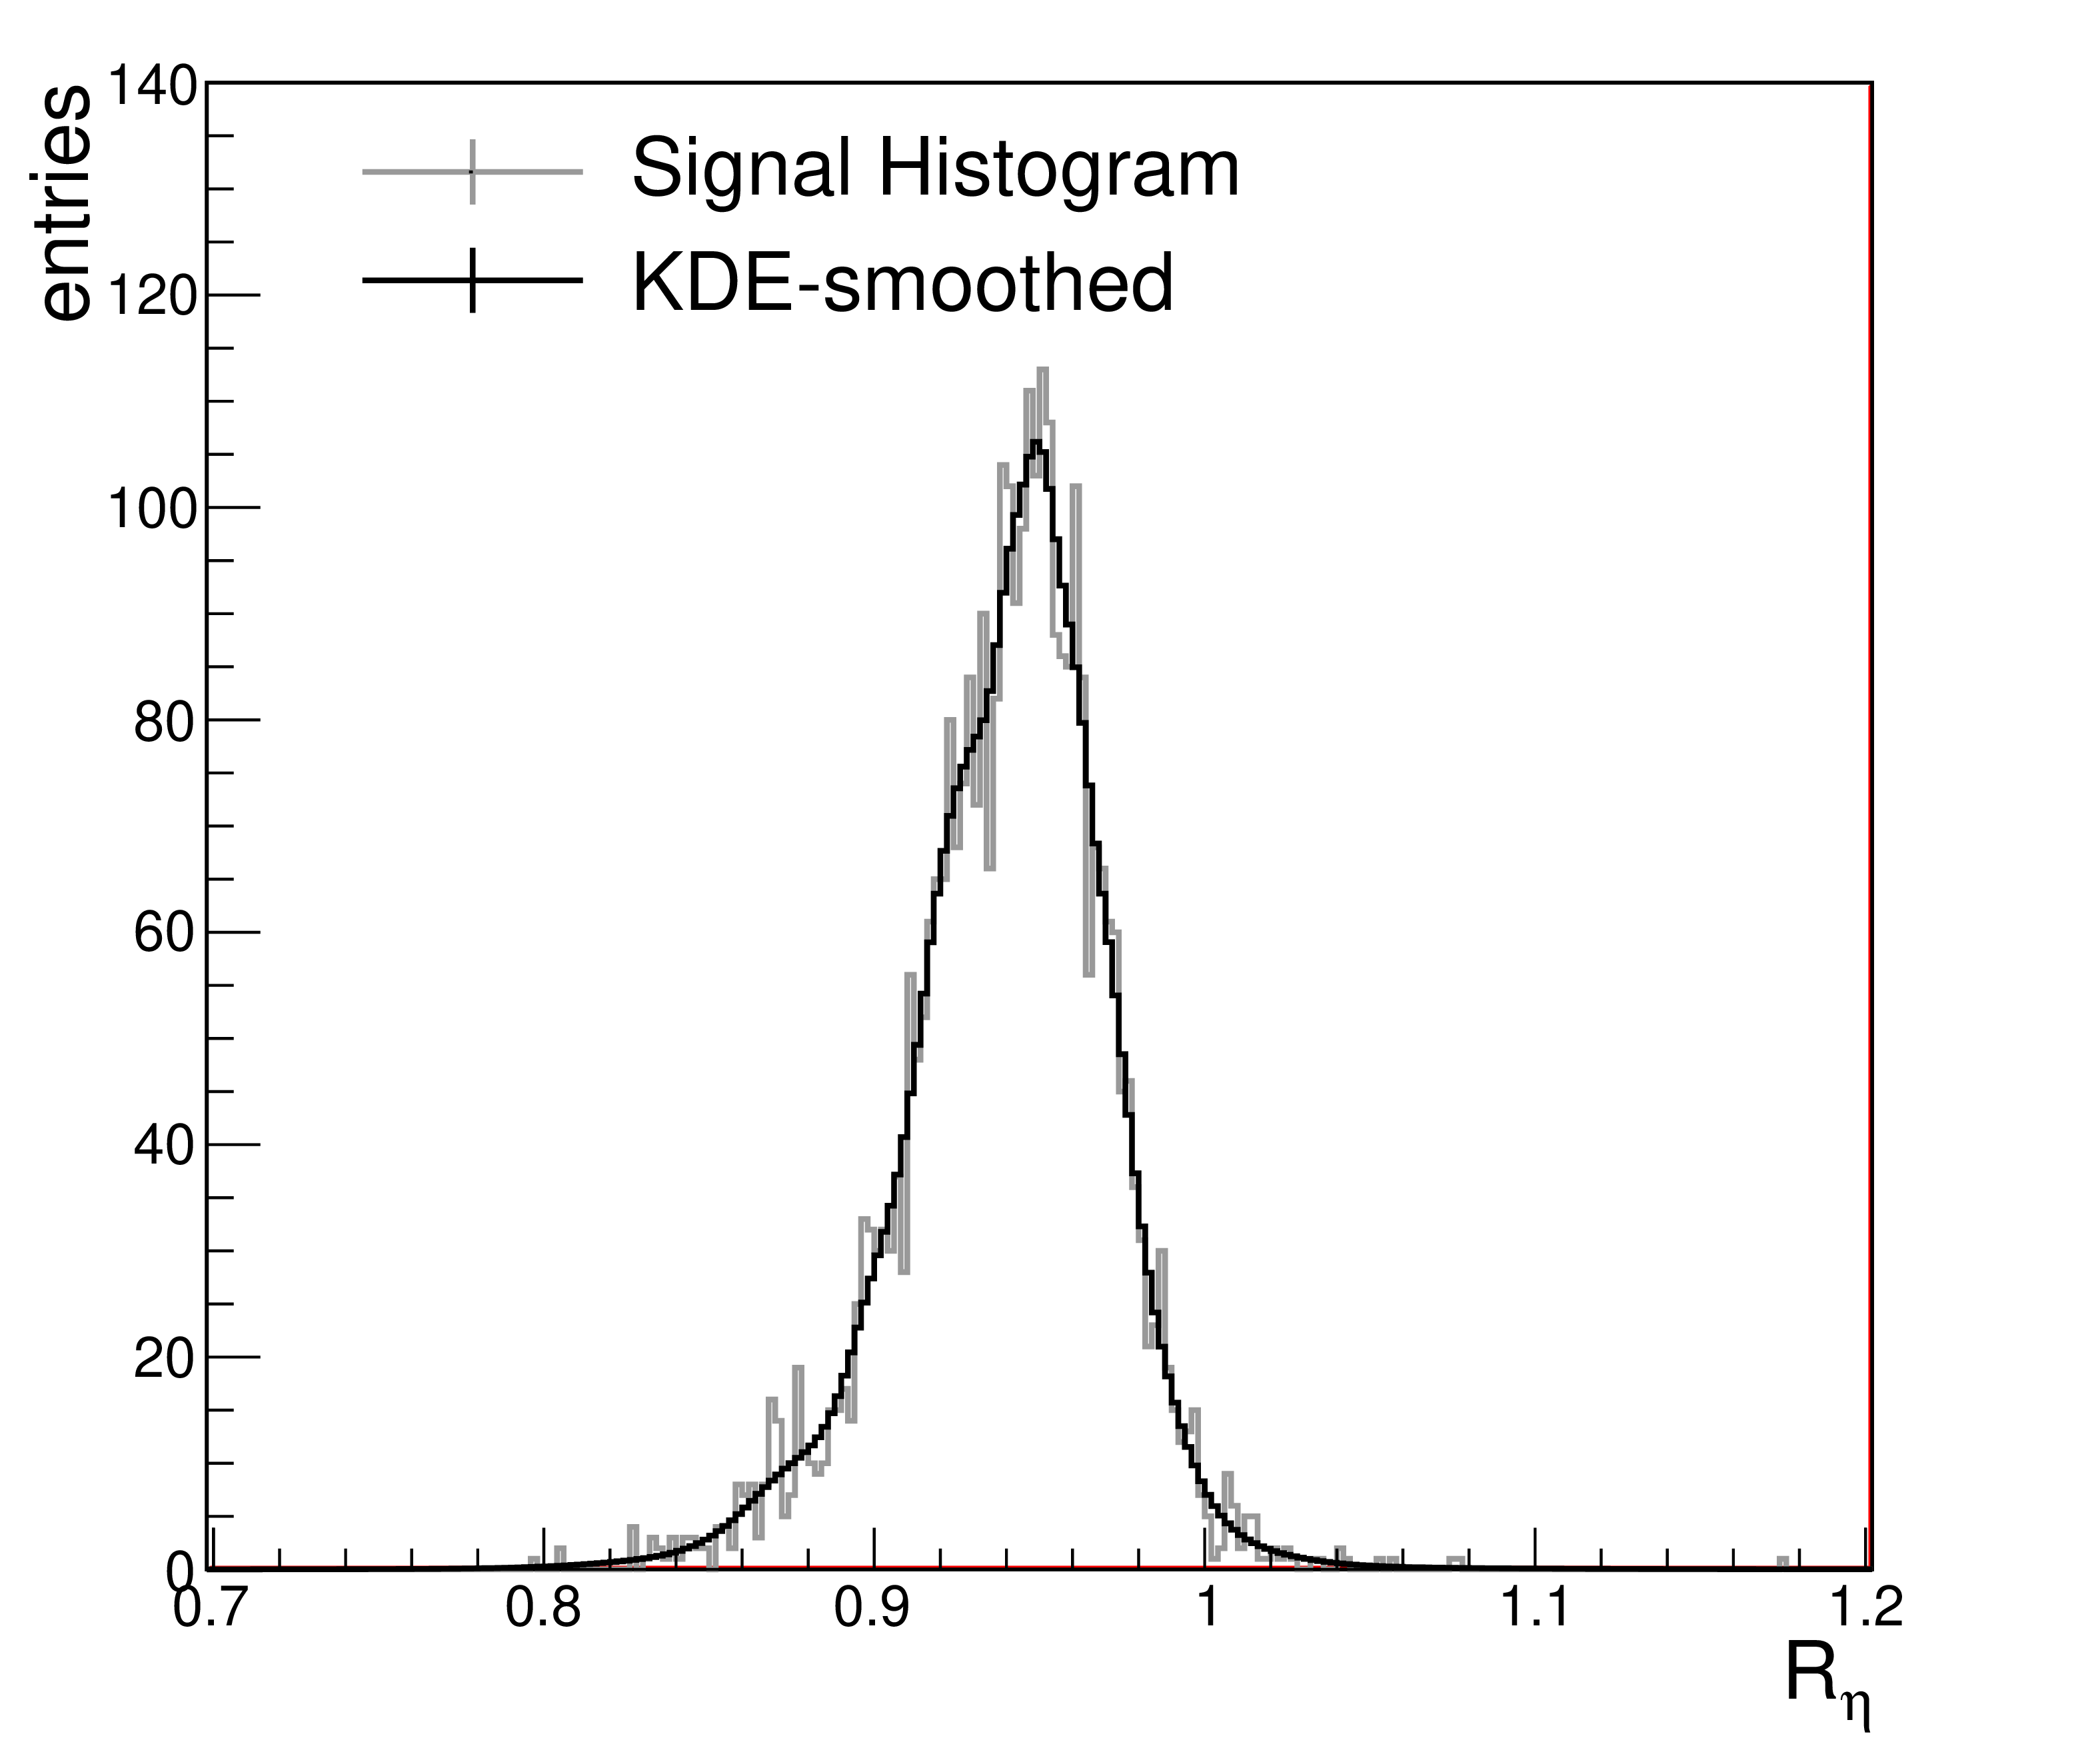
\includegraphics[width=.98\textwidth]{figs/egamma/new_kde_example.png}
      \caption{}
      \label{fig:egamma:KDEexample}
    \end{subfigure}
     \caption[The KDE method. In (a), an illustration of the advantage of the adaptive KDE pdf smoothing technique in regions with low statistics.  In (b), an example of a variable distribution and its adaptive KDE-smoothed pdf]{The KDE method. In (a), an illustration of the advantage of the adaptive KDE pdf smoothing technique in regions with low statistics.  In (b), an example of a variable distribution and its adaptive KDE-smoothed pdf~\cite{Brendlinger:2228644}.}
\label{fig:egamma:KDE}
\end{figure}
\subsection{Being Efficient in a Changing Environment}
During my time working in the e/gamma group, it was also important to adjust selection criteria to adapt to busier environments. 

%Alluded to several times in the text already, and more explicitly referenced in Section \ref{sec:egamma:LHpdfs}, is the concept of adjusting selection criteria in order to remain optimal and retain efficiency as a function of the electron's kinematics.
%For the electron identification this amounts to creating completely independent likelihoods in orthogonal regions in  \et\ and $\eta$ phase space called ``bins''.
%%%, i.e. in a particular \et/$\eta$ bin an entire set of pdfs is built from electrons that meet the particular \et and $\eta$ selection criteria for that bin.
%Additionally each bin has a linear loosening of it's discriminant value decision as a function of the pileup activity.

\subsubsection{Pileup Dependence of Discriminating Variables}
\label{sec:egamma:pileup}
%The average number of interactions per bunch crossing in $2017$ increased to $37.8$ from $25$ in $2016$ (and staying roughly the same in 2018 at 36.1, Figure \ref{fig:detector:pileupprofile}).
The wide range of pileup during Run 2 (see Figure~\ref{fig:detector:pileupprofile}) affects the discriminating variables used in the likelihood calculation.
% as could be imagined when visually comparing a pileup of 25 in Figure \ref{fig:detector:pileup25} to a pileup of 65 in Figure \ref{fig:detector:pileup65} back in Section \ref{sec:detector:lhc}.
The hadronic leakage variable, \rhad\ and the middle layer of the EM calorimeter variable, \reta, are the most affected by increases in pileup.
The shapes of these variables become wider and more elongated as is shown in Figure \ref{fig:egamma:rhadretahimu}.
Thereby becoming more background shaped in a high pileup environment, hence reducing the discriminating power of these variables.
These two variables are among the most powerful, as shown in $n-1$ likelihood studies Figure \ref{fig:egamma:nminusoneroccurve}, and thus indispensable in the likelihood variable menu.
\begin{figure}[h]
  \centering
    \begin{subfigure}[b]{0.49\textwidth}
      \centering
      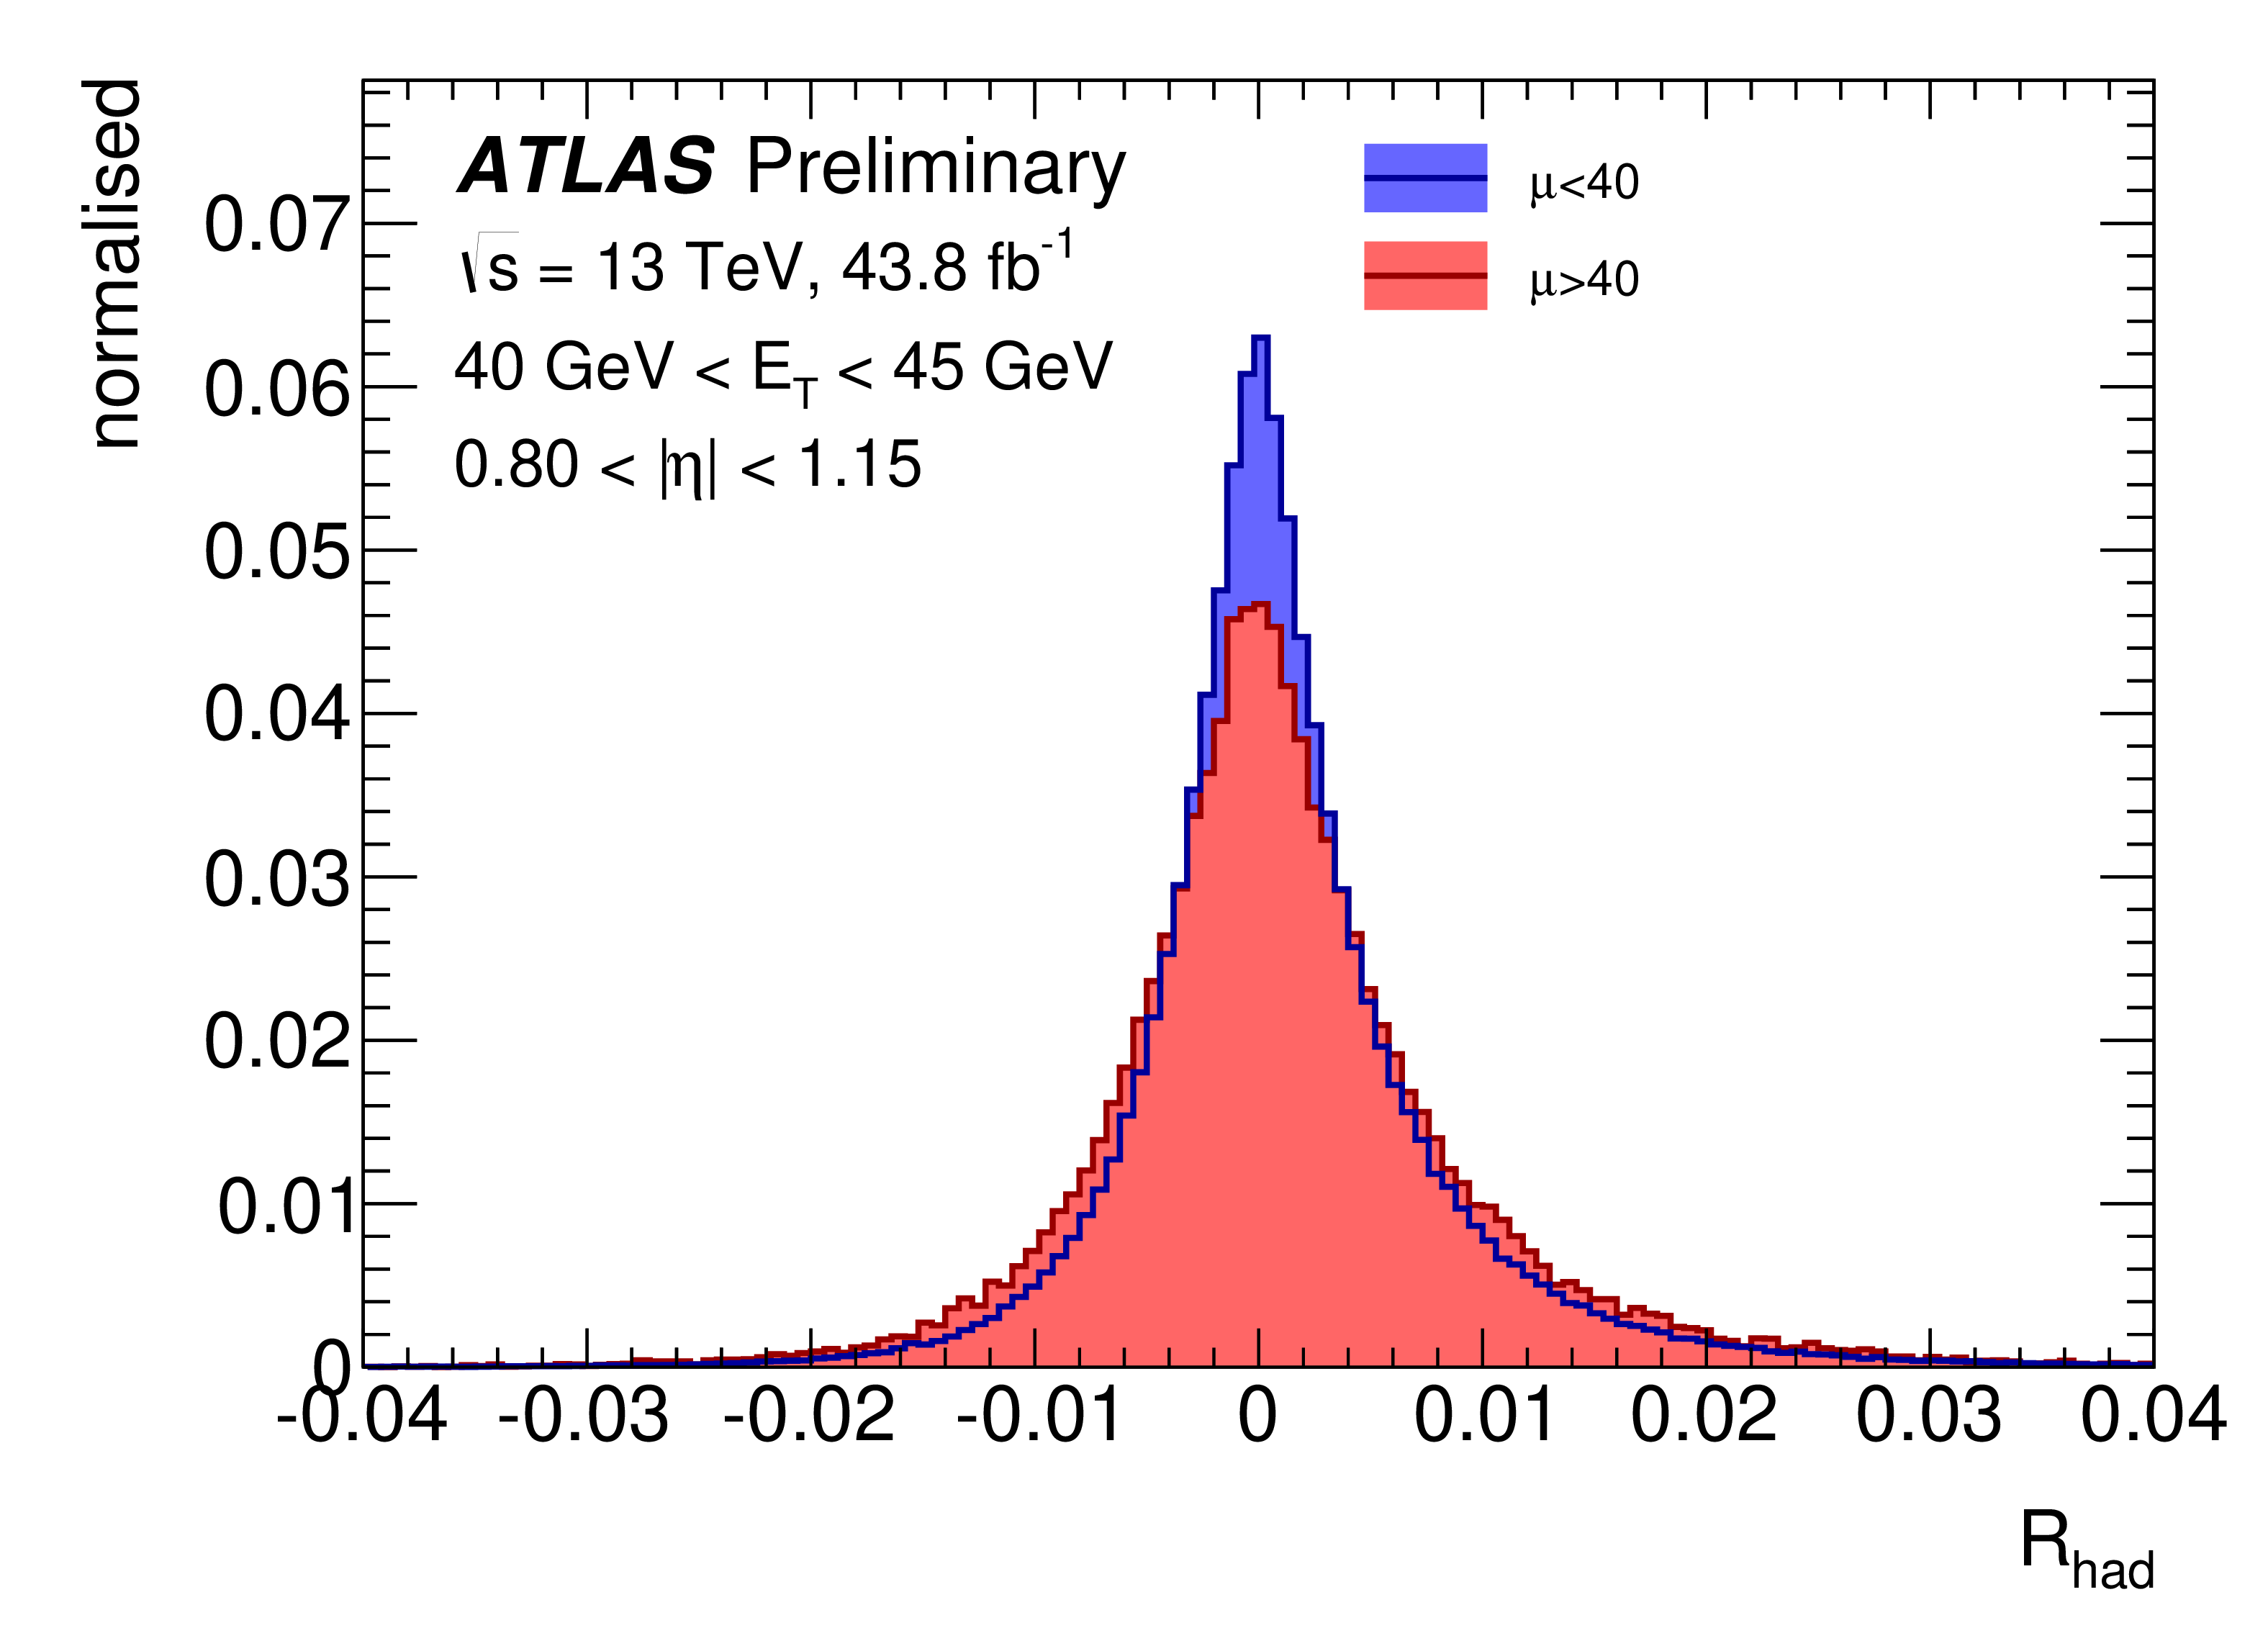
\includegraphics[width=1.02\textwidth]{figs/egamma/rhad_hilomu.png}
      \caption{}
      \label{fig:egamma:rhad_hilomu}
    \end{subfigure}
    \hfill
    \begin{subfigure}[b]{0.49\textwidth}
      \centering
      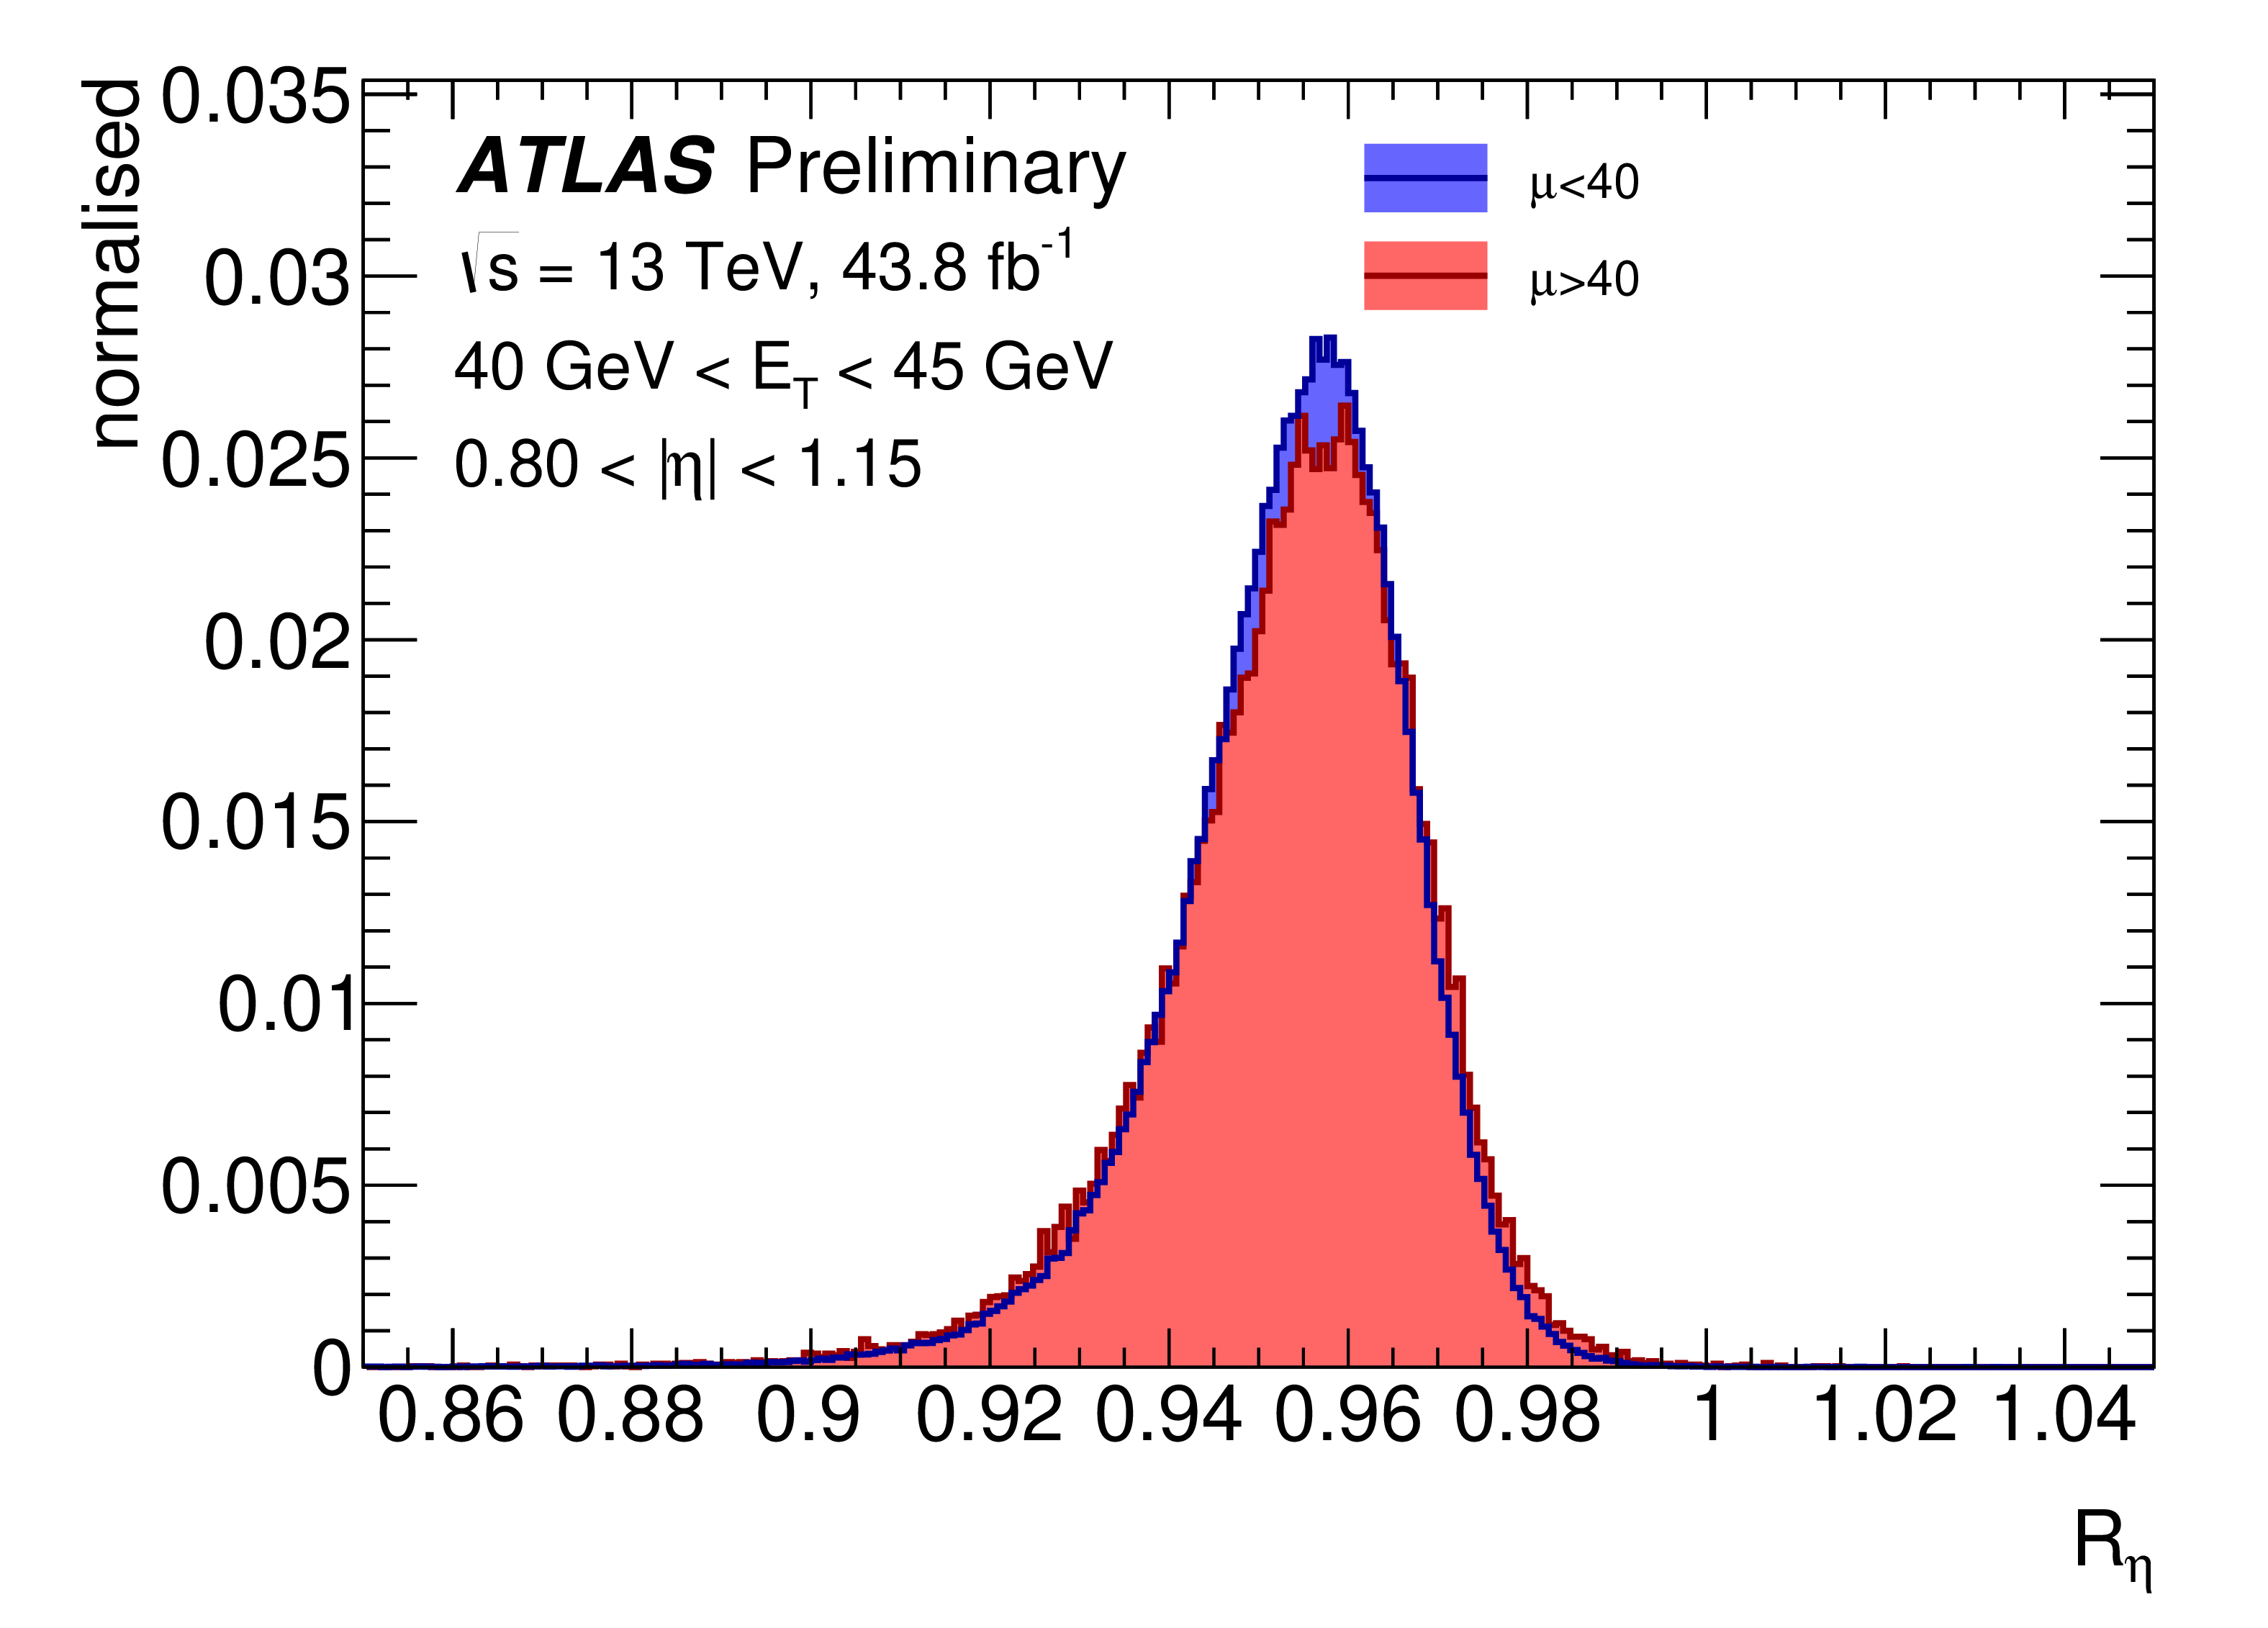
\includegraphics[width=1.02\textwidth]{figs/egamma/rphi_hilomu.png}
      \caption{}
      \label{fig:egamma:rphi_hilomu}
    \end{subfigure}
    \caption[Electron variable distributions \rhad\ and \reta\ showing high pileup's  effect on the shapes of the distributions]{Electron variable distributions for the variables \rhad\ and \reta\ are shown for electrons with 40~\GeV $<$ \et\ $<$ 45~\GeV and $0.80 < |\eta| < 1.15$.
    They have been obtained from 43.8~\ifb of data recorded in 2017 at \rts\ = 13~\TeV that were selected with $\mu >40$ (red) or $\mu<40$ (blue).
    Events were selected with a tag-and-probe method and applying a very loose selection on the likelihood discriminant used in the electron ID menu in order to reject contributions from background events.}
\label{fig:egamma:rhadretahimu}
\end{figure}
\begin{figure}[h]
\centering
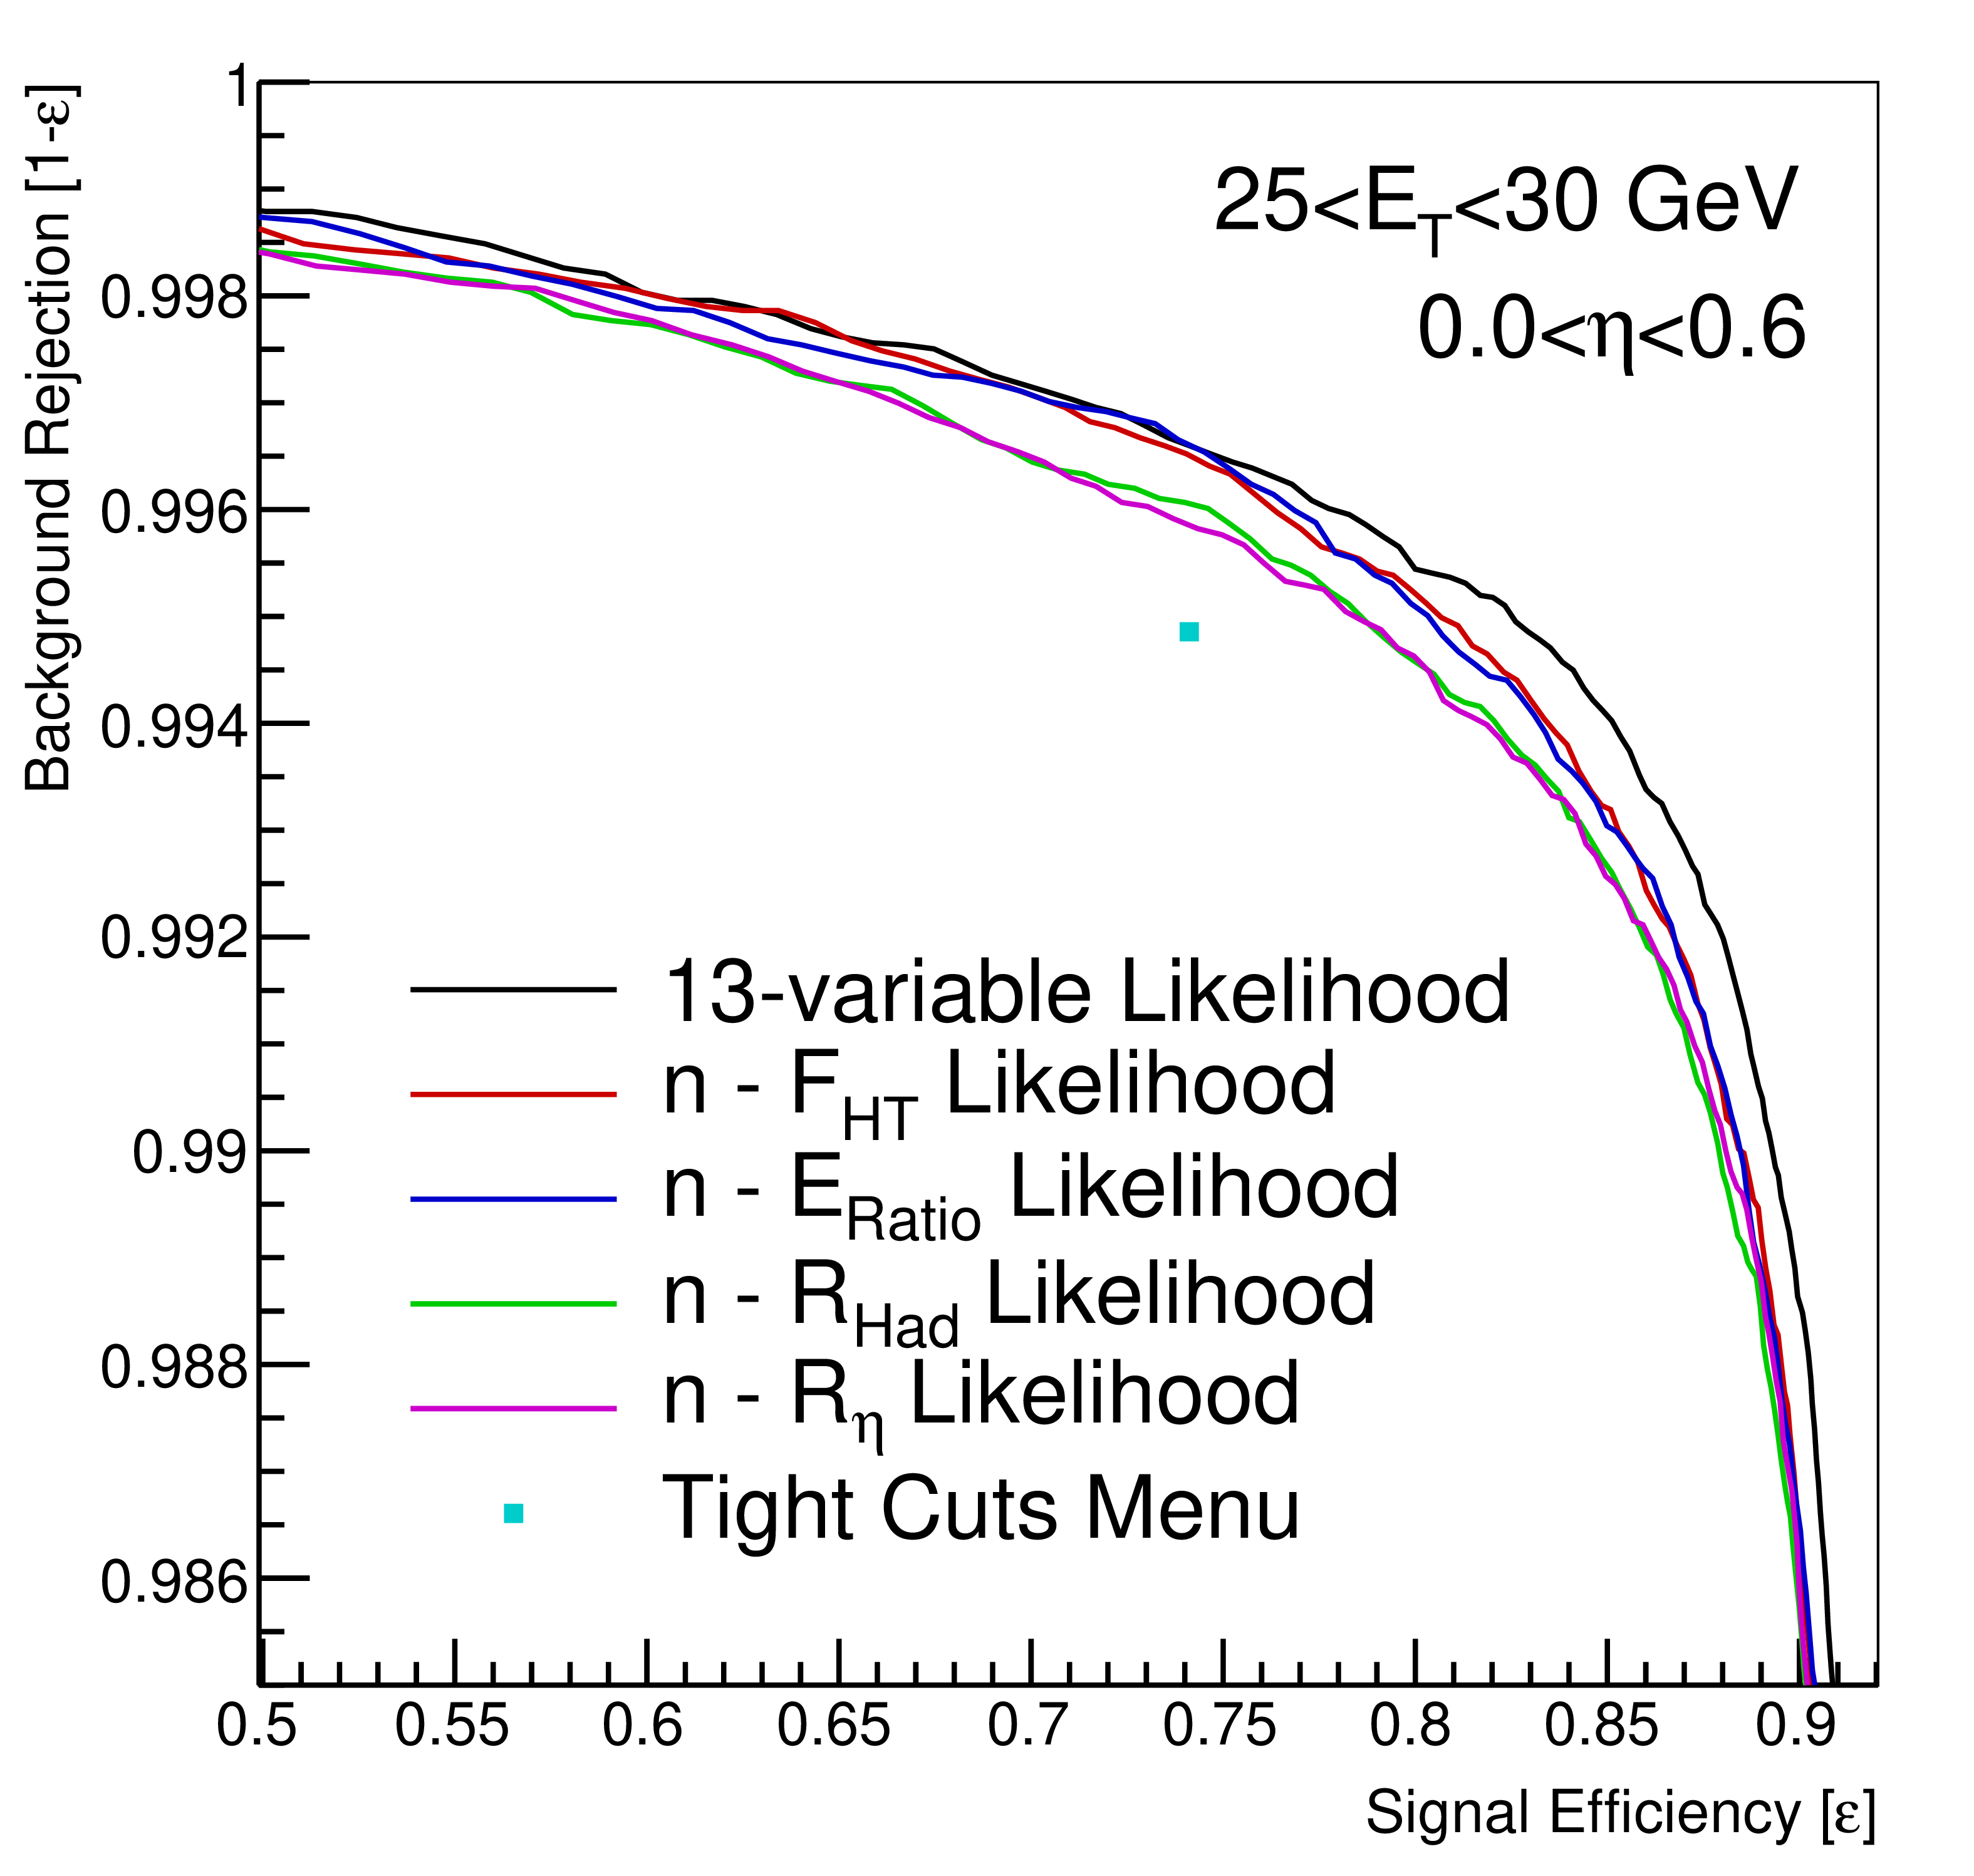
\includegraphics[width=.80\textwidth]{figs/egamma/nminus1_plot.png}
\caption[Electron LH variables $n-1$ ROC curve showing signal efficiency/background rejection response of LH when single variables are removed from the LH.]{The $n-1$ method used to optimize the choice of variables to use in the electron likelihood.
Individual variables are removed from the nominal list of likelihood variables, and the likelihood recalculated to assess the relative power of each variable.
The example shows the importance of \TRTHighTHitsRatio, \deltaEmax, \rhad\ and \reta; the performance of the likelihood decreases when each is removed.
The \Tight ~cut-based operating point is shown for comparison \cite{Brendlinger:2228644}.}
\label{fig:egamma:nminusoneroccurve}
\end{figure}
The distributions of the remaining electron discriminating variables are not largely affected by the increase in pileup. % Figures to be added
%The electron identification efficiencies at low $E_T$ show discrepancies between the high and low pile-up environments. At $\et = 15~\GeV$ low pile-up data has an electron identification efficiency of $0.68$ where as high pile-up data has an electron identification efficiency of $0.65$. At high \et, the difference between the efficiencies in high and low pile-up environments narrows. At $\et = 70~\GeV$, low pile-up data has an electron identification efficiency of $0.91$ where as high pile-up data has an electron identification efficiency of $0.90$. The impact of high pile-up on the electron identification efficiencies decreases with increasing transverse energy, \et~(Figure \ref{eff_et}).
%Additionally, the electron identification efficiencies for a high pile-up environment are consistently lower than those in a low pile-up environment across the full range of pseudo-rapidity (Figure \ref{eff_eta}).
This effect corresponds to the likelihood discriminant being systematically \emph{lower} in higher pileup conditions, leading to a negative efficiency slope as a function of the number of primary vertices, \nvtx.

In Run 1, this effect was corrected by making the discriminant cut linearly dependent on the number of vertices with the form $d(n_{\mathrm{vtx}}) = d_{\mathcal{L}} - a\cdot n_{\mathrm{vtx}}$ in each \et/$\eta$ bin.
Introducing this discriminant dependence on \nvtx\ softens the resulting effect of \nvtx ~on the signal efficiency.
It should be noted that the \rhad\ and \reta\ distributions are broader in the background, and thus the background response is less dependent on \nvtx.
As a result, correcting the signal efficiency causes the background to develop an \nvtx\ dependence, with worse rejection at higher \nvtx.
%In fact, a perfectly corrected signal efficiency in the \Tight\ regime results in an untenably strong \nvtx\ dependence in background rejection, as 
This is illustrated by the black markers in Figure \ref{fig:egamma:nvtxDepBackground}.
\begin{figure}[h]
\centering
    \begin{subfigure}[b]{0.49\textwidth}
      \centering
      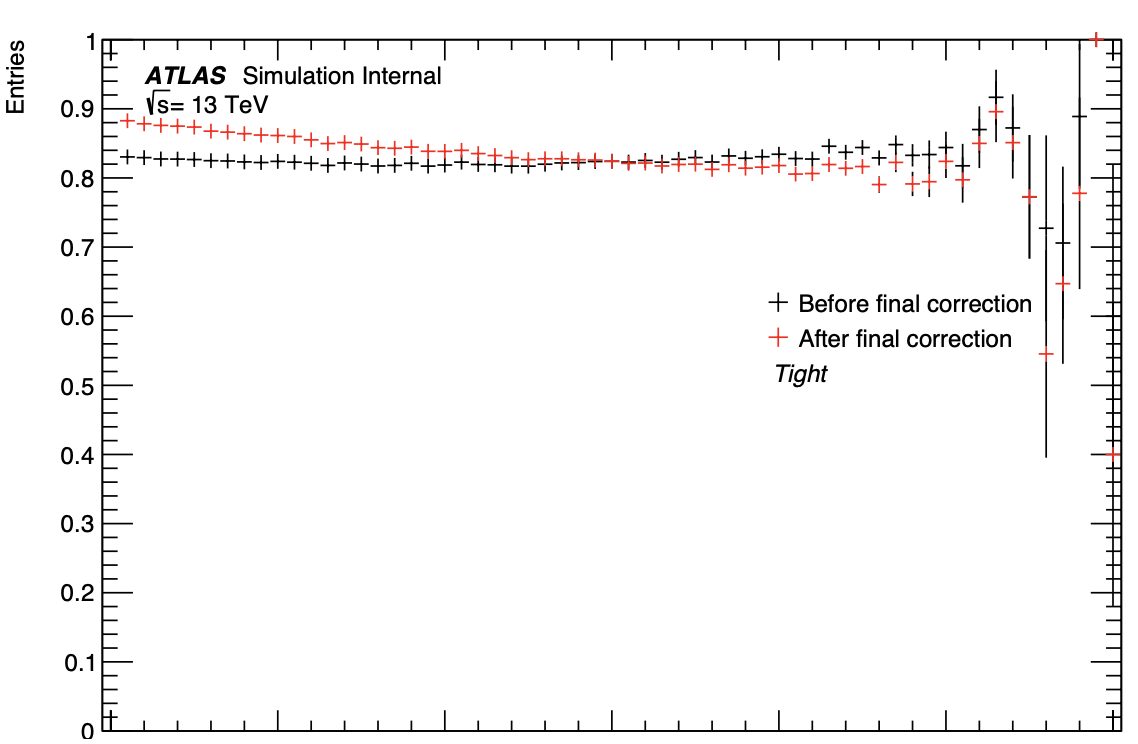
\includegraphics[width=1.0\textwidth]{figs/egamma/nvtxdepSignal.png}
      \caption{}
      \label{fig:egamma:nvtxDepSignal}
    \end{subfigure}
    \hfill
    \begin{subfigure}[b]{0.49\textwidth}
      \centering
      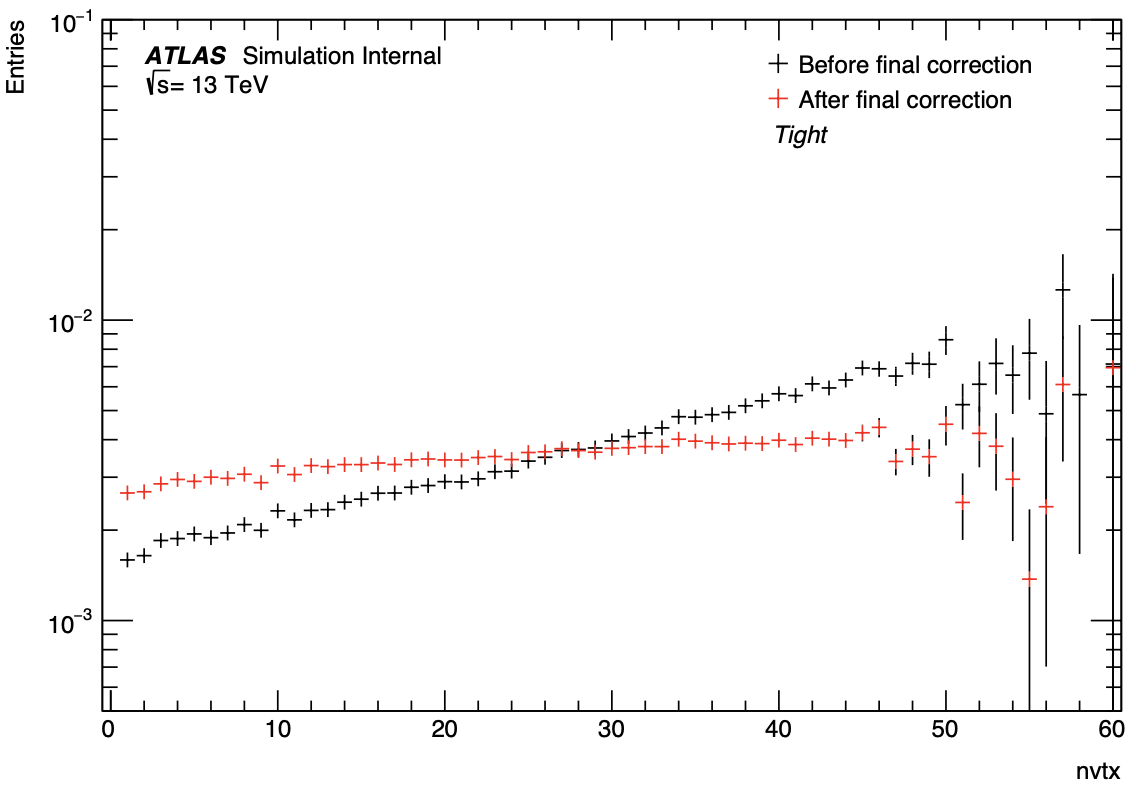
\includegraphics[width=1.0\textwidth]{figs/egamma/nvtxdepBackground.png}
      \caption{}
      \label{fig:egamma:nvtxDepBackground}
    \end{subfigure}
    \caption[Illustration of the identification efficiency dependence of (a) signal and (b) background on \nvtx\ for the \Tight\ operating point.]{Illustration of the identification efficiency dependence of (a) signal and (b) background on \nvtx\ for the \Tight\ operating point. 
    %The black points are the using exactly the discriminant as transformed by the method detailed in Section \ref{sec:egamma:pileup} whereas the red points are after a final by-hand correction in order to balance the competing effect of a large positive background dependence on \nvtx. 
    %The correction is applied directly to $a$ so the subset nature of the LH is maintained.
    }
    \label{fig:egamma:nvtxDep}
\end{figure}
%The chosen values for $d_{\mathcal{L}}$ balance these competing effects (red markers in Figure \ref{fig:egamma:nvtxDep}) and the resulting behavior matches that of the corresponding 2012 cut-based menus.
An additional correction is applied to balance these competing effects and is shown by the red markers in Figure~ \ref{fig:egamma:nvtxDep}.
In the end, these \nvtx\ dependent cuts on the likelihood output are only applied for \Medium\ and \Tight\ operating points. 
The dependence of the efficiency on the pile-up for the \Loose\ and \VeryLoose\ operating points were deemed to be small enough to not warrant a correction.
However, this meant that on rare occasions, the operating points were not perfect subsets of one another, since \Medium\ and \Tight\ could become looser than \Loose\, for instance, as seen in Figure \ref{fig:egamma:subset}.
\begin{figure}[h]
\centering
    \begin{subfigure}[b]{0.49\textwidth}
      \centering
      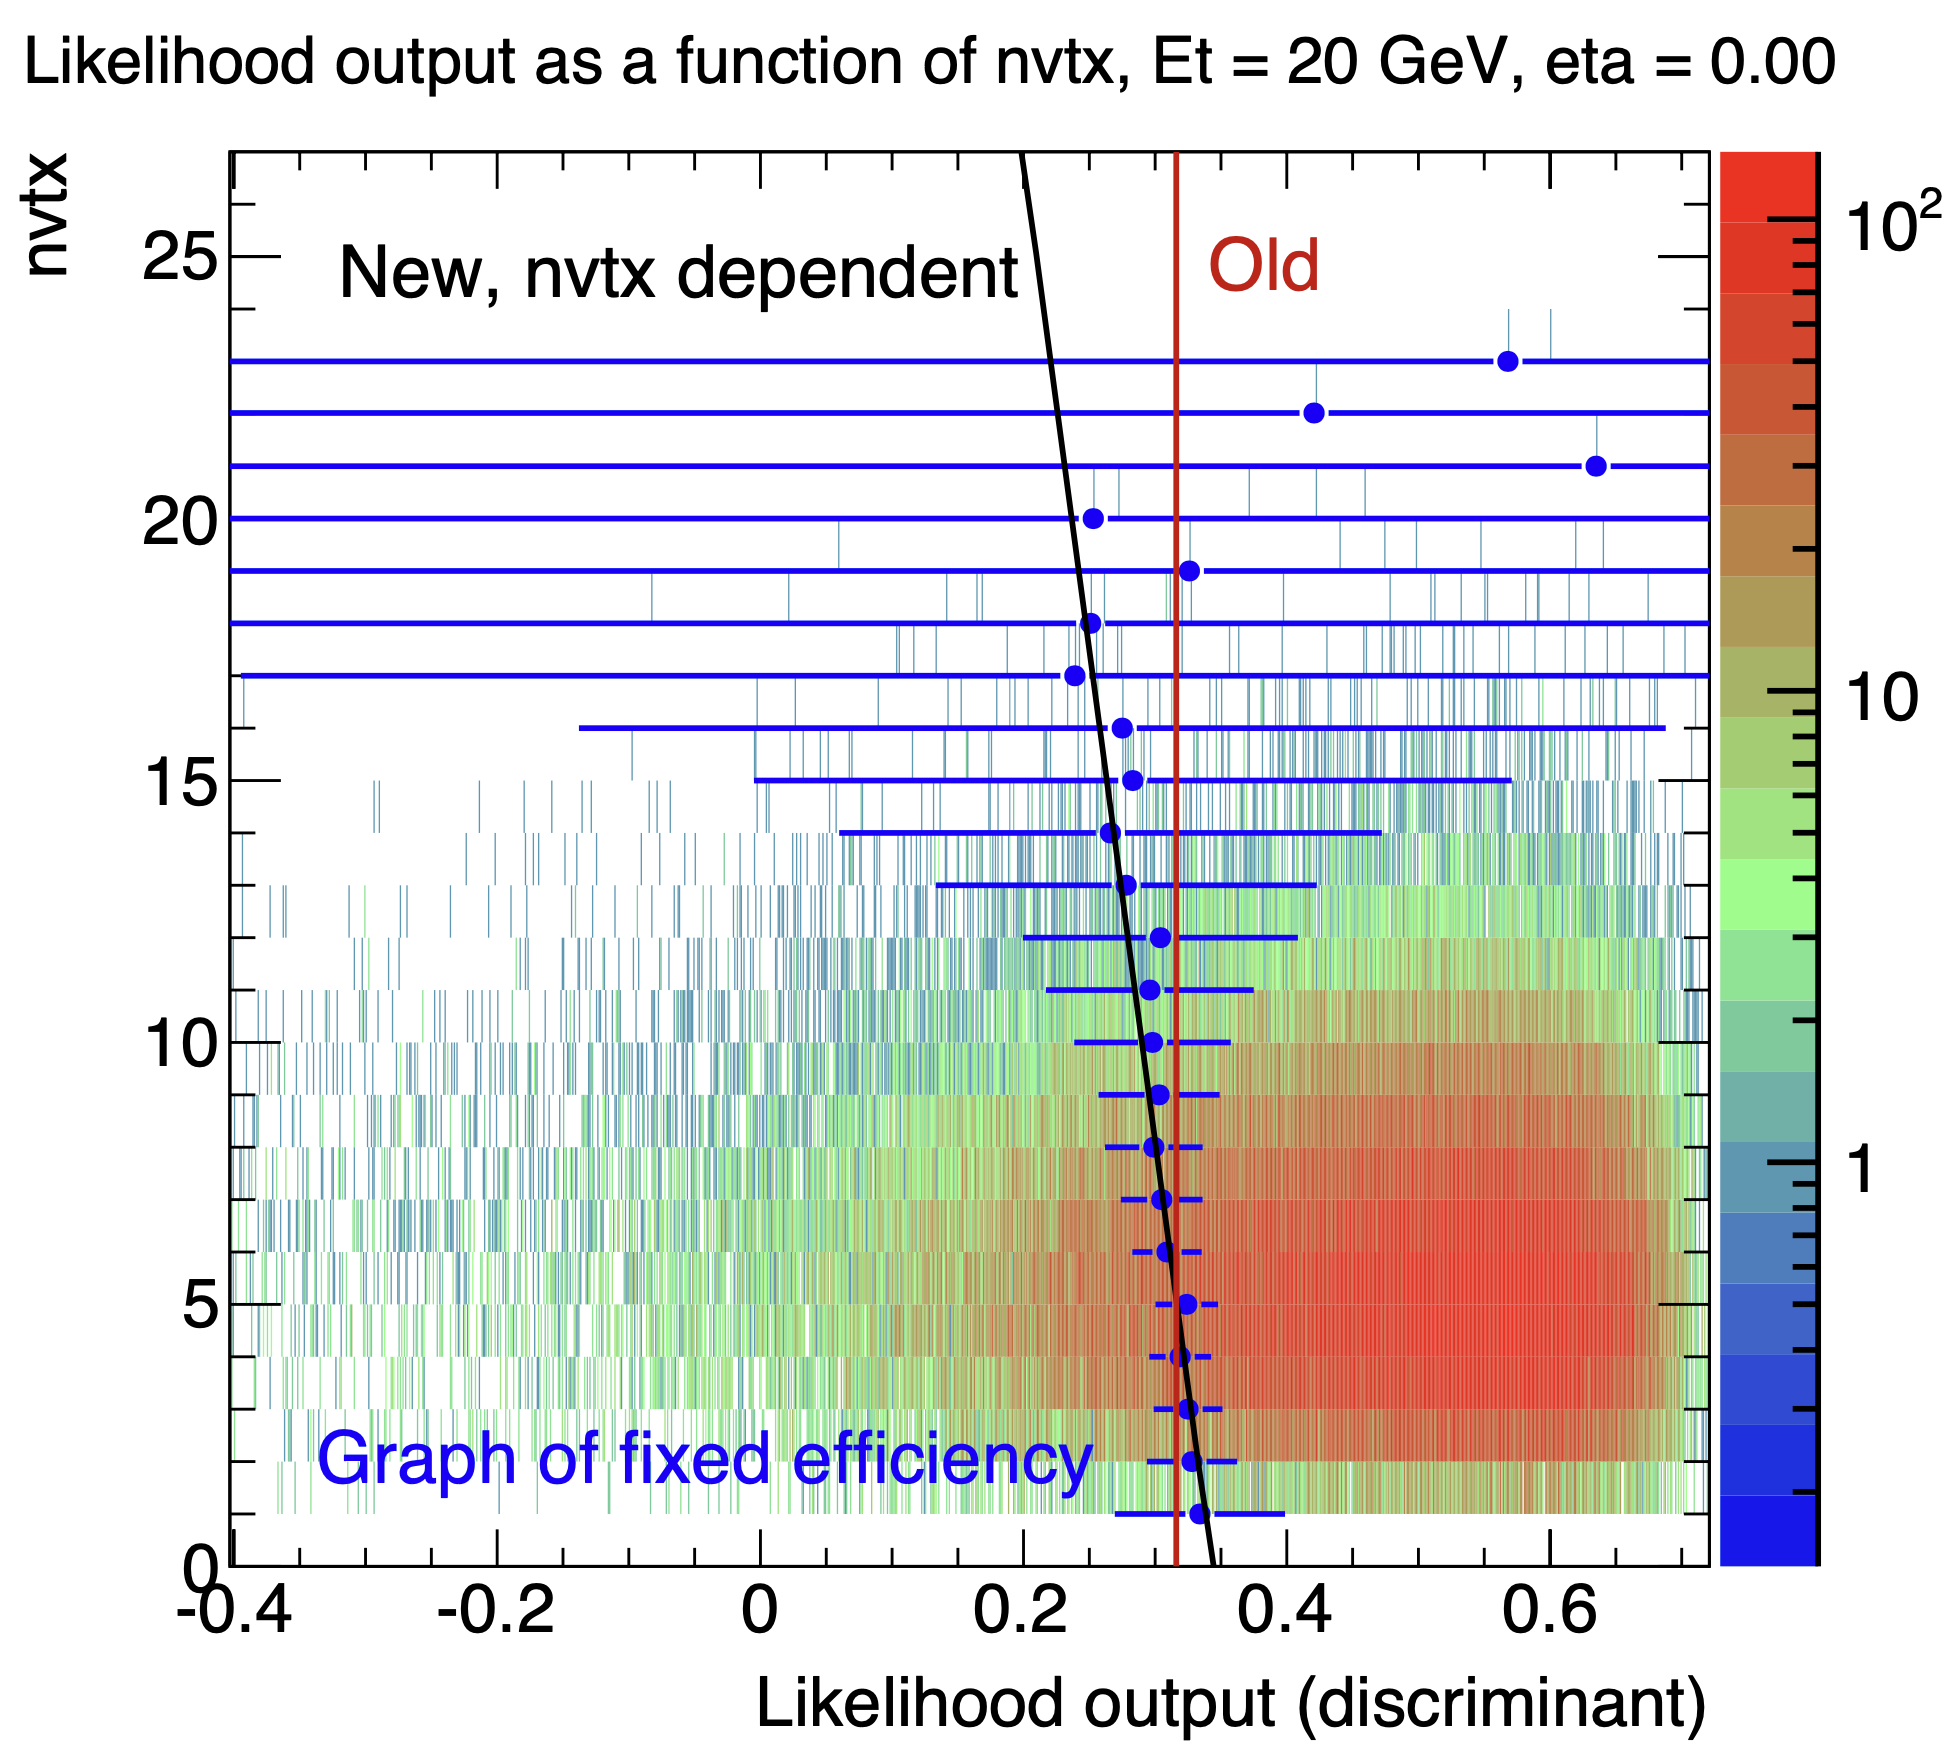
\includegraphics[width=1.0\textwidth]{figs/egamma/equiEfficiency.png}
      \caption{}
      \label{fig:egamma:equiEfficiency}
    \end{subfigure}
    \hfill
    \begin{subfigure}[b]{0.49\textwidth}
      \centering
      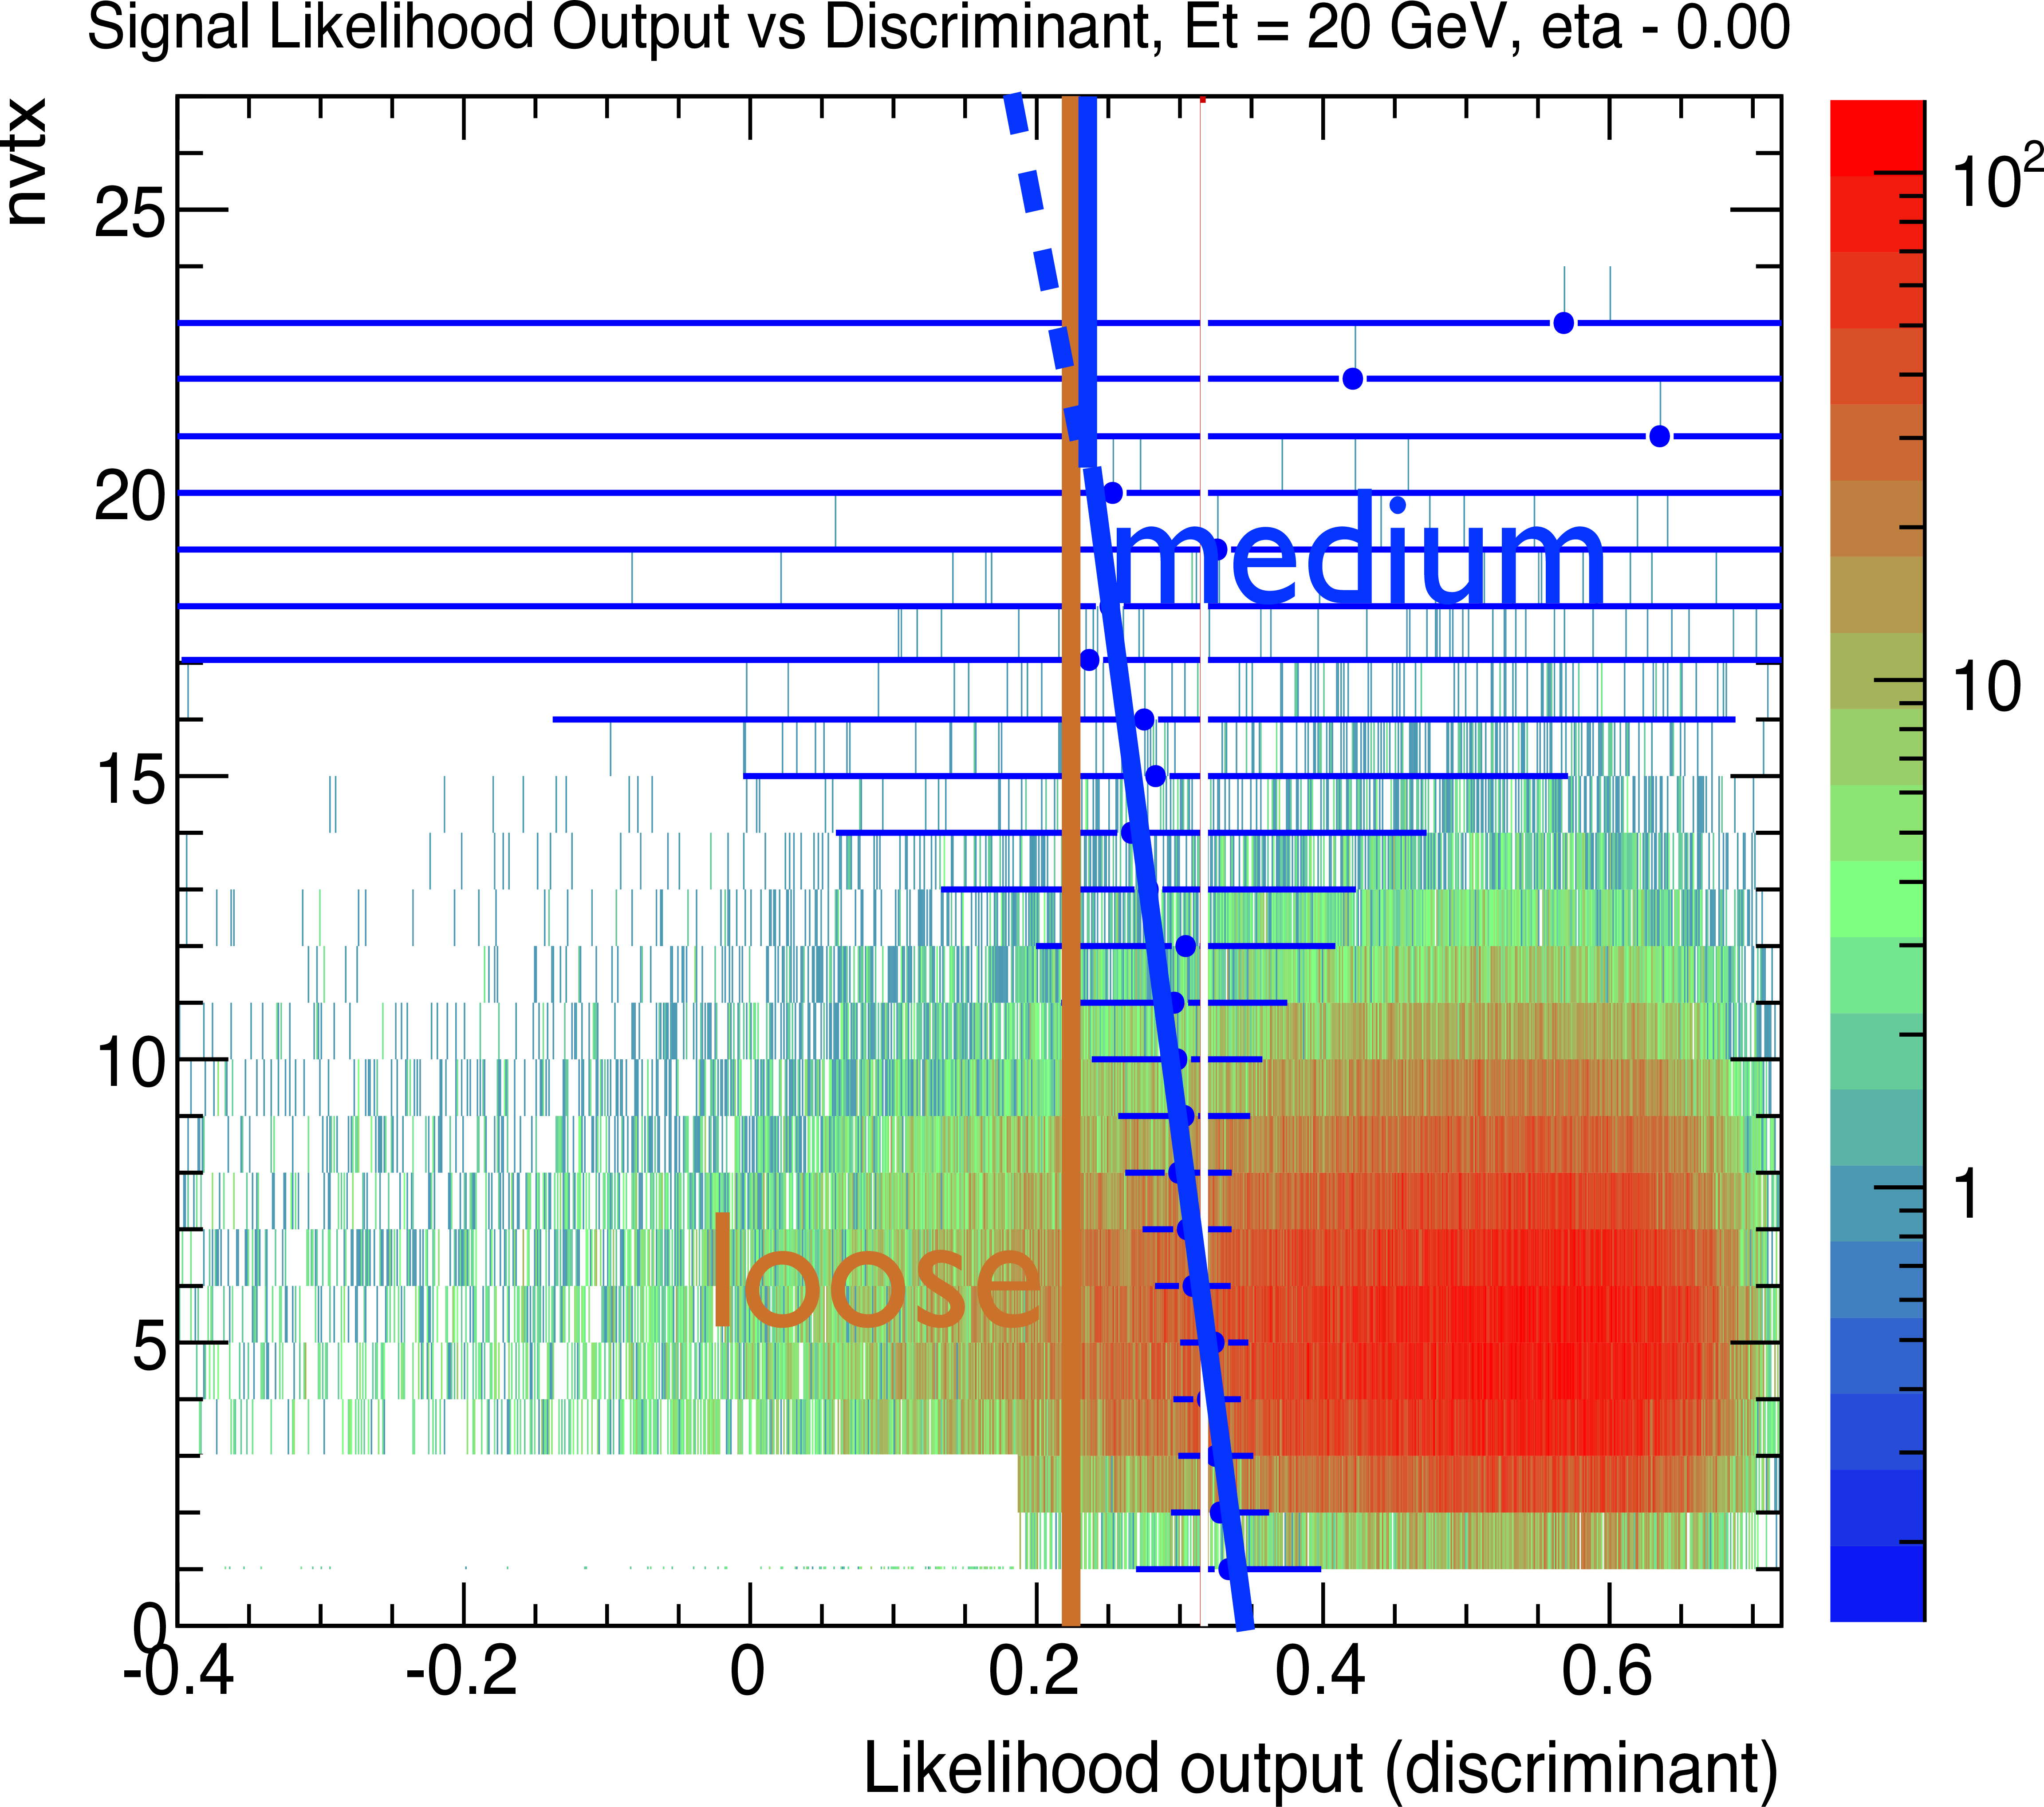
\includegraphics[width=1.0\textwidth]{figs/egamma/nvtx.png}
      \caption{}
      \label{fig:egamma:subset}
    \end{subfigure}
    \caption[Example of the pileup correction used in Run-1 where the z-axis shows the number of entries in each bin.]{Example of the pileup correction used in Run-1 where the z-axis shows the number of entries in each bin. 
    (a) Shows what a flat discriminant cut looks like and as well as a discriminant cut adjusted as a function of \nvtx to maintain a constant signal efficiency.
    (b) The blue dashed line shows that with large pileup, the \Medium\ operating point could be looser than the \Loose\ operating point, so they are not perfect subsets.
    The solid blue line shows what is desired, namely, for \Medium\ to always be a subset of \Loose.}
    \label{fig:egamma:pile-up}
\end{figure}
While this was typically a $10^{-5}$ effect or less, it was not desirable to repeat this for Run-2.

A different strategy was employed in Run-2 to ensure that all of the tighter operating points are subsets of the looser operating points, for 2015.
Rather than directly loosening the discriminant cut value, the pileup correction was put directly into the discriminant itself.
In other words, the cut value used for each operating point is unaffected (the cuts do not change with pileup so they are subsets by construction), but with increasing pileup, the value of the discriminant changes instead. 
Mathematically, this is done as follows:
\begin{equation}
    d_{\mathrm{{\scriptsize T}\tiny{IGHT},new}}(n_{\mathrm{vtx}}) = d_{\mathrm{{\scriptsize T}\tiny{IGHT},old}} - a \cdot max(n_{\mathrm{vtx}}, n_{vtx,\text{max}})
\end{equation}
Where tight refers to the \Tight\ operating point, so the result of a cut on $d_{\mathrm{{\scriptsize T}IGHT,new}}(n_{\mathrm{vtx}})$ is identical to the Run-1 pileup-corrected cut.
To cut this off at some value of \nvtx, rather than to loosen the discriminant indefinitely, $n_{\mathrm{vtx}} {}_{,\text{max}}$ is defined as the largest value to use for the correction.
As an example, if $n_{\mathrm{vtx}} {}_{,\text{max}}$ = 50 (which it does for 2015, and increased to 100 in 2018), then the pileup correction used for all larger values of \nvtx\ will be identical, to avoid loosening the discriminant too much.
This is illustrated for $n_{\mathrm{vtx}} {}_{,\text{max}}$ = 50 as the solid blue line in Figure \ref{fig:egamma:subset}.
\begin{figure}[h]
\centering
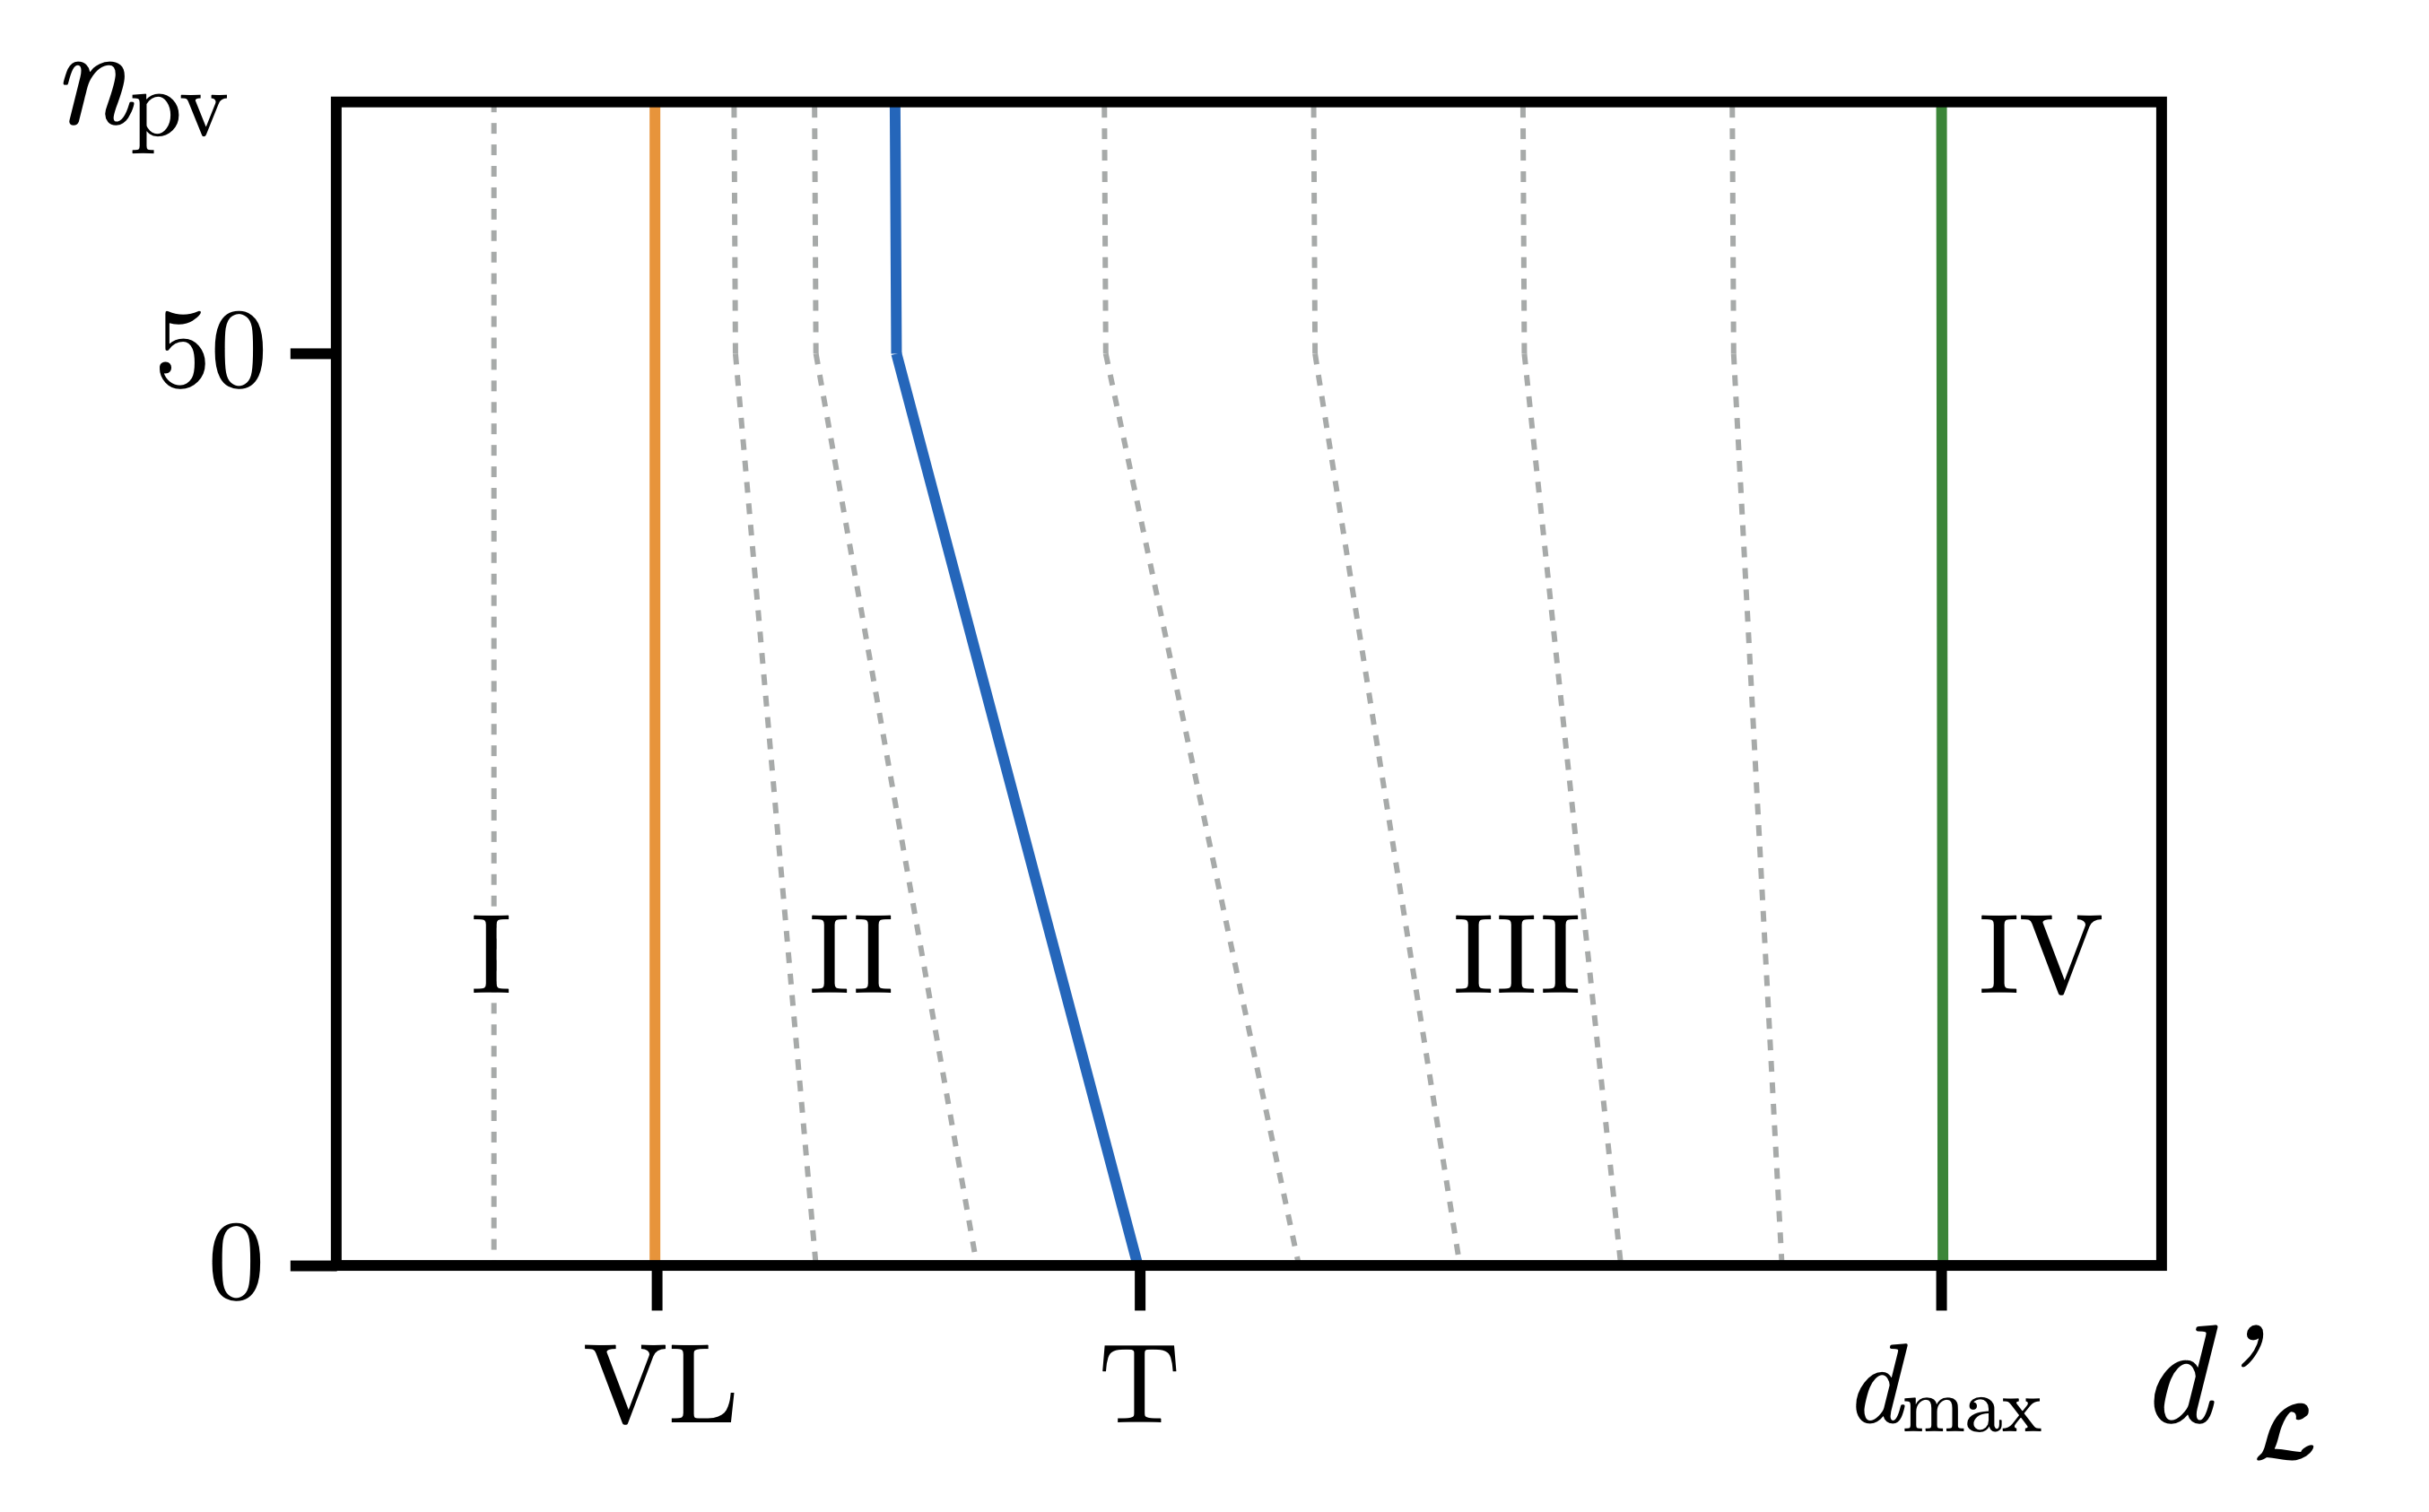
\includegraphics[width=.80\textwidth]{figs/egamma/pileupCorrection.png}
\caption[The regions I, II, III, and IV illustrate the piece-wise transform described in Section~\ref{sec:egamma:pileup}]{Sketch of the phase space carved out by the \nvtx\ dependant discriminant decisions which define the operating points \Tight\ (blue line) and \VeryLoose\ (orange line).
The regions I, II, III, and IV illustrate the piece-wise transform described in this section~\cite{Brendlinger:2228644}.}
\label{fig:egamma:piecewise}
\end{figure}
Then we define the new discriminant with a piece-wise function, continuous at each boundary condition, so:
\makebox[\textwidth]{\parbox{1.4\textwidth}{%
\begin{equation*}
\renewcommand{\arraystretch}{1.3}
 d_\text{new}(n_{vtx}) = 
  \left\lbrace
  \begin{array}{llc}
     d, & d < d_{\text{V{\tiny ERY}L{\tiny OOSE}}}  & \text{(I)} \\
     d_{\text{V{\tiny ERY}L{\tiny OOSE}}} + (d - d_{\text{V{\tiny ERY}L{\tiny OOSE}}}) \times \frac{d_{\text{{\scriptsize T}\tiny{IGHT},old}} - d_{\text{{\scriptsize V}\tiny{ERY}{\scriptsize L}\tiny{OOSE}}}}{d_{\text{{\scriptsize T}\tiny{IGHT},new}} - d_{\text{{\scriptsize V}\tiny{ERY}{\scriptsize L}\tiny{OOSE}}}}, & d_{\text{V{\tiny ERY}L{\tiny OOSE}}} \leq d < d_{\text{ T{\tiny IGHT},new}}  & \text{(II)} \\
     d_{\text{ T{\tiny IGHT},old}} + (d - d_{\text{T{\tiny IGHT},new}}) \times \frac{d_{\text{max}} - d_{\text{{\scriptsize T}\tiny{IGHT}}}}{d_{\text{max}} - d_{\text{{\scriptsize T}\tiny{IGHT},new}}}, & d_{\text{T{\tiny IGHT},new}} \leq d < d_{\text{max}}  & \text{(III)} \\
     d, & d_{\text{max}} \leq d  & \text{(IV)}
   \end{array}
   \right.
\end{equation*}
}}
Where $d_{\mathrm{\text{V{\tiny ERY}L{\tiny OOSE}}}}$ is the \VeryLoose\ operating point where no pileup correction is desired, $d_{\text{max}}$ is the largest discriminant value for which the transform should take place, which was chosen to be 2.0.
This new method of pileup correction was found to perform similarly to the correction performed in Run-1, while fixing the effect of the operating points not being subsets of one another.
%Other options were available to achieve the same effect, but this was deemed to be the simplest to technically implement, while remaining flexible enough to add additional operating points.
One small difference this introduces is that \Loose\ now depends on pileup (as \VeryLoose\ is the reference point used for loose), but the correction is smallest for the looser operating points.
Figure~\ref{fig:egamma:piecewise} illustrates how the phase space is carved out corresponding to the Roman numerals in the piece-wise equation above.

\subsubsection{Alternative pileup measures: TRT Local Track Occupancy}\label{sec:egamma:TRTTrackOcc}
In an effort to better model the local pileup activity around an electron I investigated if parameterizing the pileup correction in terms of the newly available TRT local track occupancy variable, which measures activity around the electron, could provide improved performance in replacing the event-by-event offline measure of the number of primary vertices \nvtx.
Additional motivation for the TRT local track occupancy lies in its availability \emph{online} as well.
As the availability of pileup measure information is limited online since event reconstruction is required to determine the number of primary vertices, \nvtx.
%This variable must be substituted at the HLT with a different variable.
The nominal replacement is the average number of collision vertices $\langle \mu \rangle$, measured online by a set of luminosity detectors (one dedicated detector LUCID, the Beam Conditions Monitor, and measurements from the Tile and Forward calorimeters and the ID) it is the average over all BCIDs in a Luminosity Block\footnote{The time unit in which ATLAS luminosity data is recorded, an interval during which the luminosity is supposed to remain constant} (one minute of data taking). The TRT local track occupancy could then mitigate inefficiencies arising from the use of different variables online and offline.
The local TRT occupancy is measured in 192 regions (32 sectors in phi for the barrel, endcap A and endcap B regions on each side of the detector).
For each track, the number of hits in each region is weighted by the local TRT occupancy\footnote{The occupancy is number of TRT straws which have a low-level hit within a validity gate divided by the total number of live TRT straws in the region considered} to calculate the local occupancy around the track.  
%First defining the general TRT occupancy:
%\begin{equation}
%    \frac{\text{number of TRT straws which have a low-level hit within a validity gate}}{\text{total number of live TRT straws}}
%\end{equation}
%The Local Track Occupancy is then given by the following equation:
%\begin{equation}
%    \text{Local Track Occupancy} = \textstyle \frac{\sum_{i=region}^{192} L_{i} \cdot n_{i}}{\sum_{i=region}^{192} n_{i}}
%\end{equation}
%Where $L_{i}$ is the occupancy in a region defined as the number of straws registering a hit in the region divided by the total number of straws in that region.
%Where $L_{i}$ is the occupancy in a region.
%There are 192 regions defined by 32 $\phi$ sectors in all 6 partitions (barrel, endcap type-A and endcap type-B for both sides)
%And $n_i$ is the number of track hits in that region.
\begin{figure}[h]
\centering
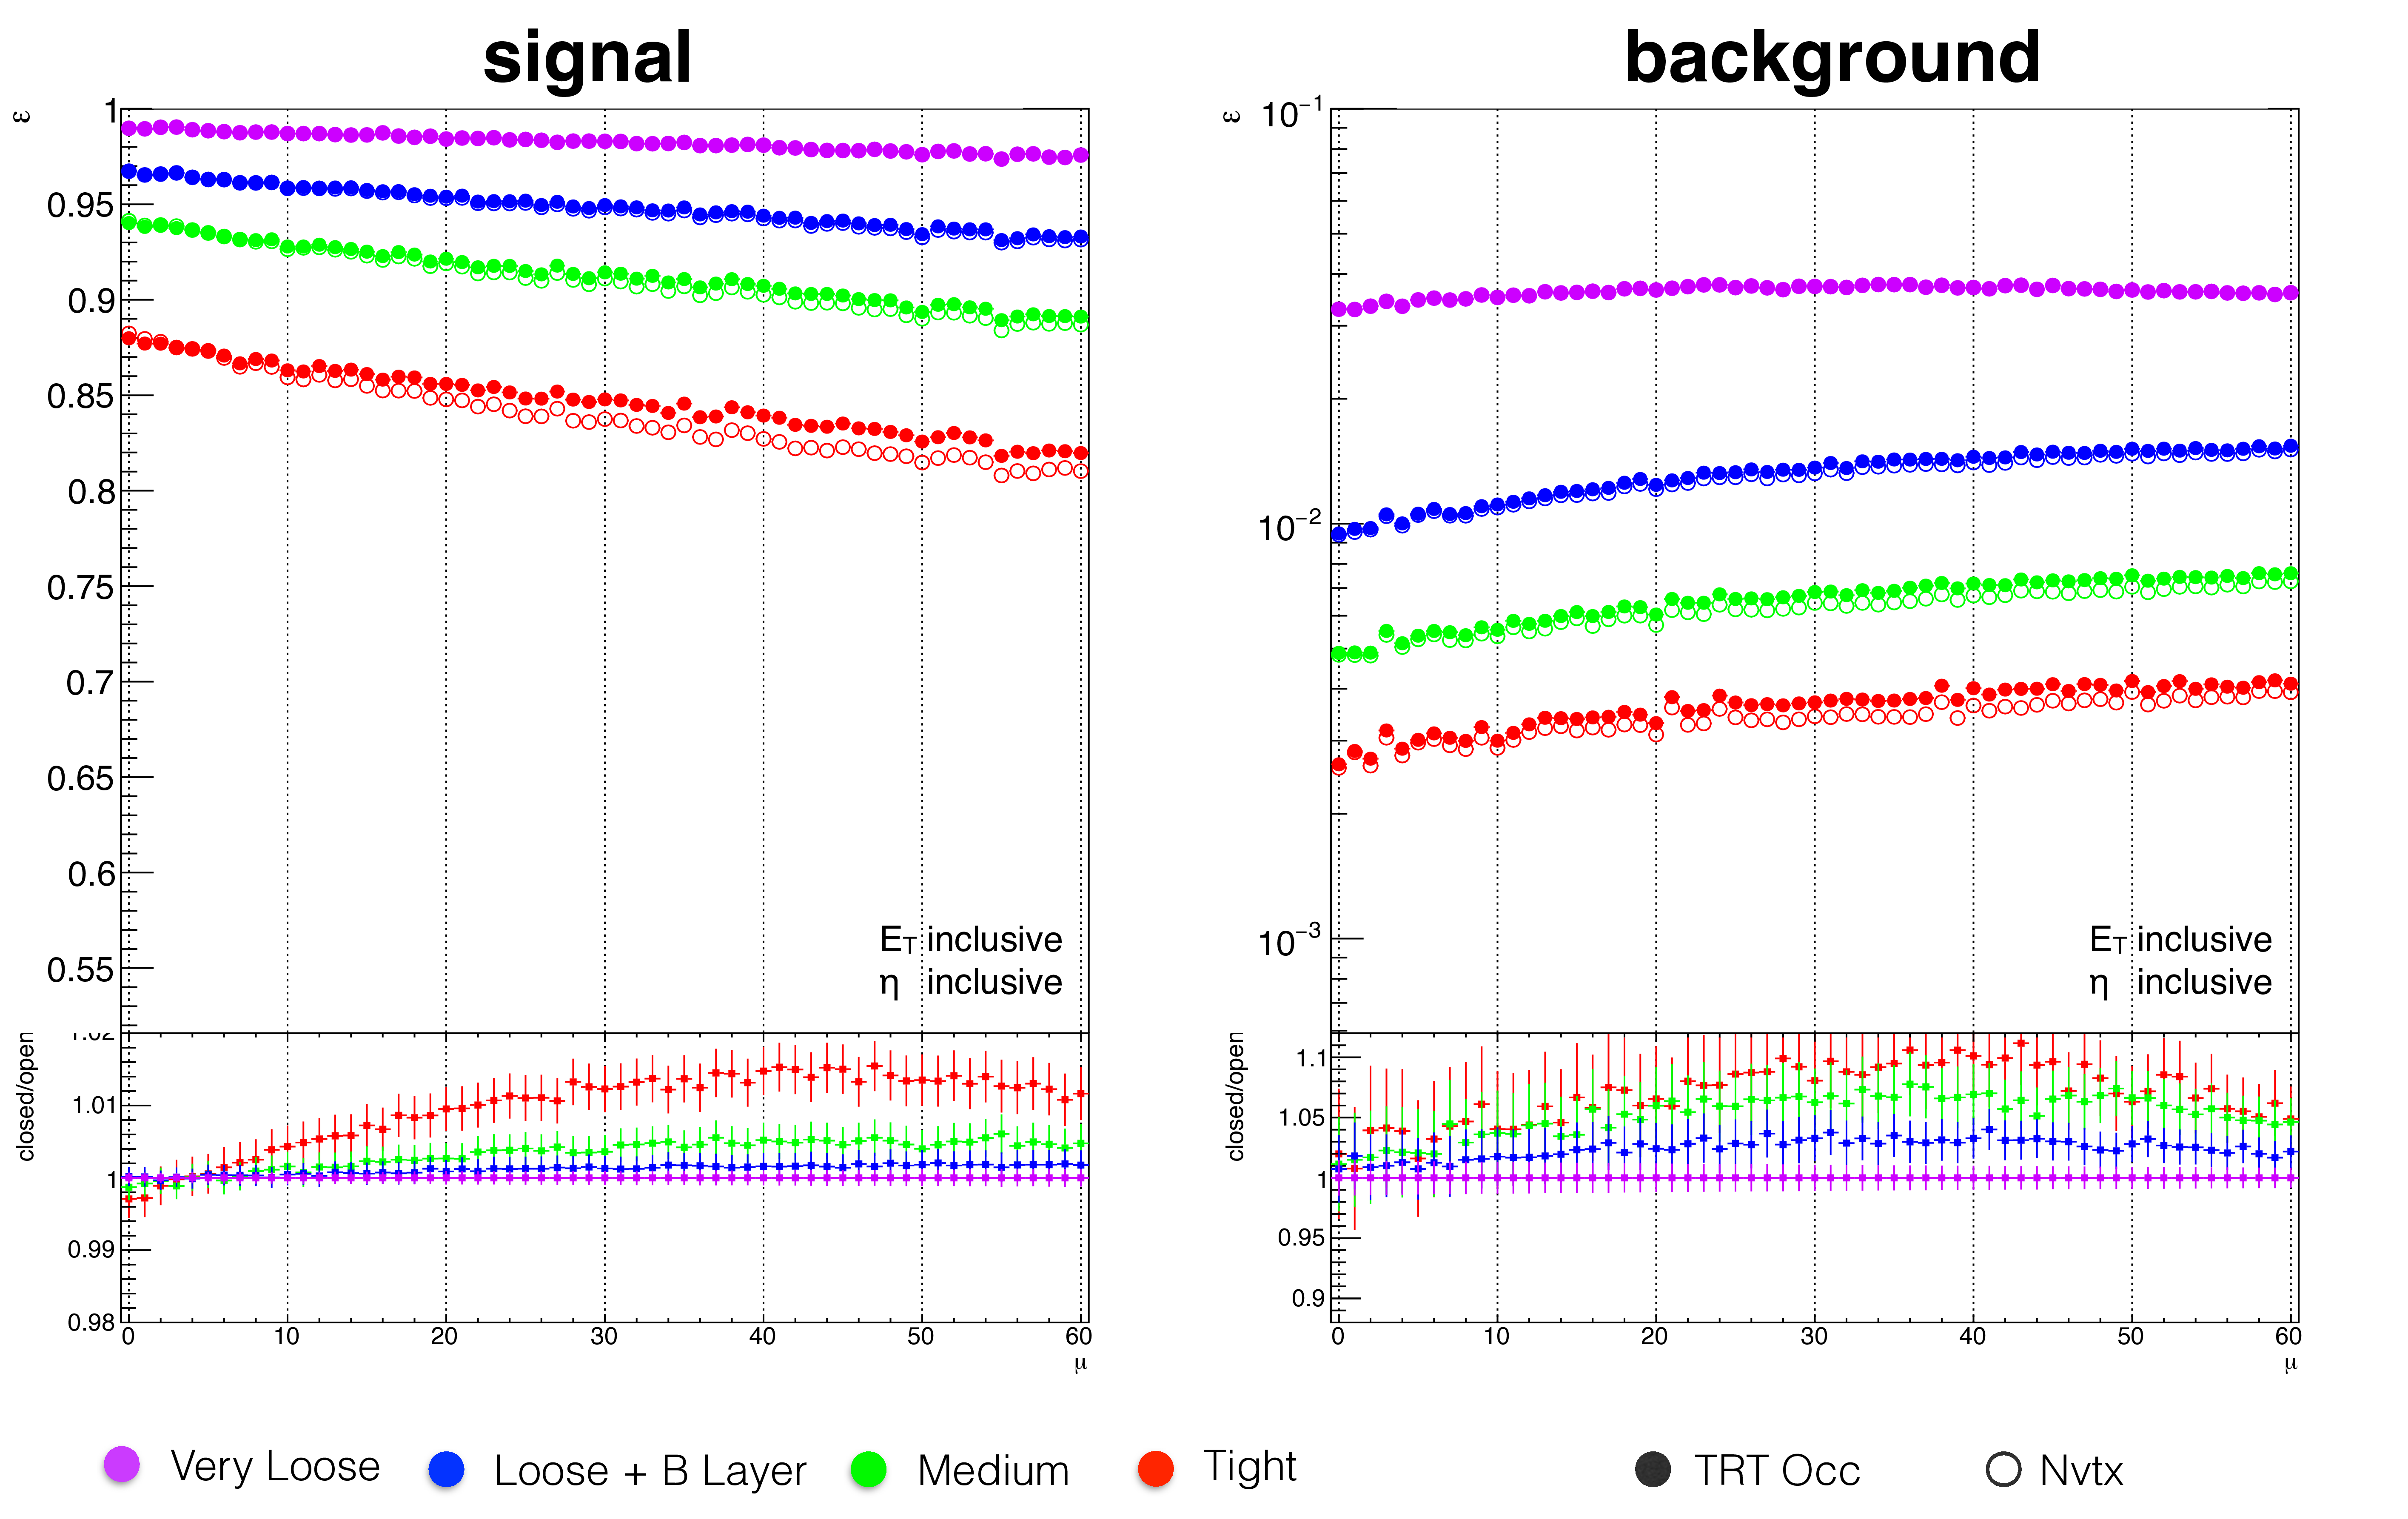
\includegraphics[width=.95\textwidth]{figs/egamma/TRTLocalTrackOcc.png}
\caption[Signal (a) and background (b) identification efficiencies as a function of the nominal electron LH discriminant pileup measure \nvtx\ and the alternate variable local TRT track occupancy.]{Signal (a) and background (b) identification efficiencies as a function of the nominal electron LH discriminant pileup measure \nvtx\ and the alternate variable local TRT track occupancy are shown for nominal LH menu \Tight, \Medium, \Loose, and \VeryLoose\ operating points.
In the bottom panels the efficiencies for the local TRT track occupancy to \nvtx\ is shown.
}
\label{fig:egamma:TRTLocalTrackOcc}
\end{figure}
The TRT local track occupancy was implemented in the relevant software tools in the same manner as \nvtx\ and $\mu$ with several technical caveats.
Firstly, the TRT acceptance only covers an $|\eta|<2.01$ requiring the original measures to be used for the most forward two $\eta$ bins. 
Second `silicon-only'' tracks are possible where no TRT hits are registered for the electron object leading to an undefined local track occupancy which not desirable, again the original measures are defaulted to in this special case. 
In Figure~\ref{fig:egamma:TRTLocalTrackOcc} the local track occupancy is compared to \nvtx\ in MC, both signal and background efficiencies are shown as a function of $\mu$.
%The signal is a combination of sample of \Zee\ and \Jee\ MC for the high (\Et$>$15~\gev) and low (\et$<$15~\gev) \et\ regions respectively.
%A dijet MC sample is used for background.
%Unfortunately no clear advantage in signal efficiency to background rejection was seen when using the Occupancy over \nvtx\ as a replacement for the offline pileup correction.
At most an improvement of 1\% is seen in signal efficiency for the \Tight\ operating point, while in background an overall reduction in background rejection is seen, climbing to nearly a 10\% loss in rejection power for large $\mu$.
This result can be understood as for signal the TRT Local track occupancy variable is correlated with pileup, so the signal efficiency improves slightly, but for background there is a stronger correlation with more activity from the other particles from a jet.
While the TRT local track occupancy was attractive as a variable available online and offline, the increase in background efficiency was extremely unattractive as it would have increased the trigger rate.

\subsection{Tuning the Electron LH}\label{sec:egamma:tuning}
A so-called ``\tune'' is defined as a set of operating points all relying on the same set of pdfs. 
The defining of an operating point is then determined by tuning to a discriminant value that results in a desired identification efficiency.
And just as kinematic bins are necessary for the pdfs, these are needed for the discriminant requirements as well.
The $|\eta|$ and \Et\ bins used for the likelihood discriminant requirements are shown in Table~\ref{tab:etabins} and the second row of Table~\ref{tab:etbins} respectively.
Note that fewer \Et\ bins are used for the pdfs than for the discriminant requirements; this is to allow for a smoother increase of electron efficiency with \et\ than would otherwise occur.
As a general improvement to the electron likelihood with respect to Run 1, an interpolation procedure was implemented to interpolate the pdfs and discriminant cut values between the \et\ bins defined for the operating points.
This procedure, first introduced for analysis of 2015–2016 data, allows for better continuity of electron identification efficiency as a function of \et\ when using \et\ bins that are finer than that used for the identification optimization (which have a bin width of 5~\GeV or larger for \et\ $>$ 10~\GeV).
The discriminant tuning procedure is then done in each bin independently using MC, in order to get a pure enough sample of electrons, that are modified with data-to-simulation shift and width corrections.
Examples of these corrections are illustrated in Figure ~\ref{fig:egamma:data_MC_comparison_shifts}
\begin{figure}[t]
\centering
\begin{subfigure}[b]{0.49\textwidth}
\centering
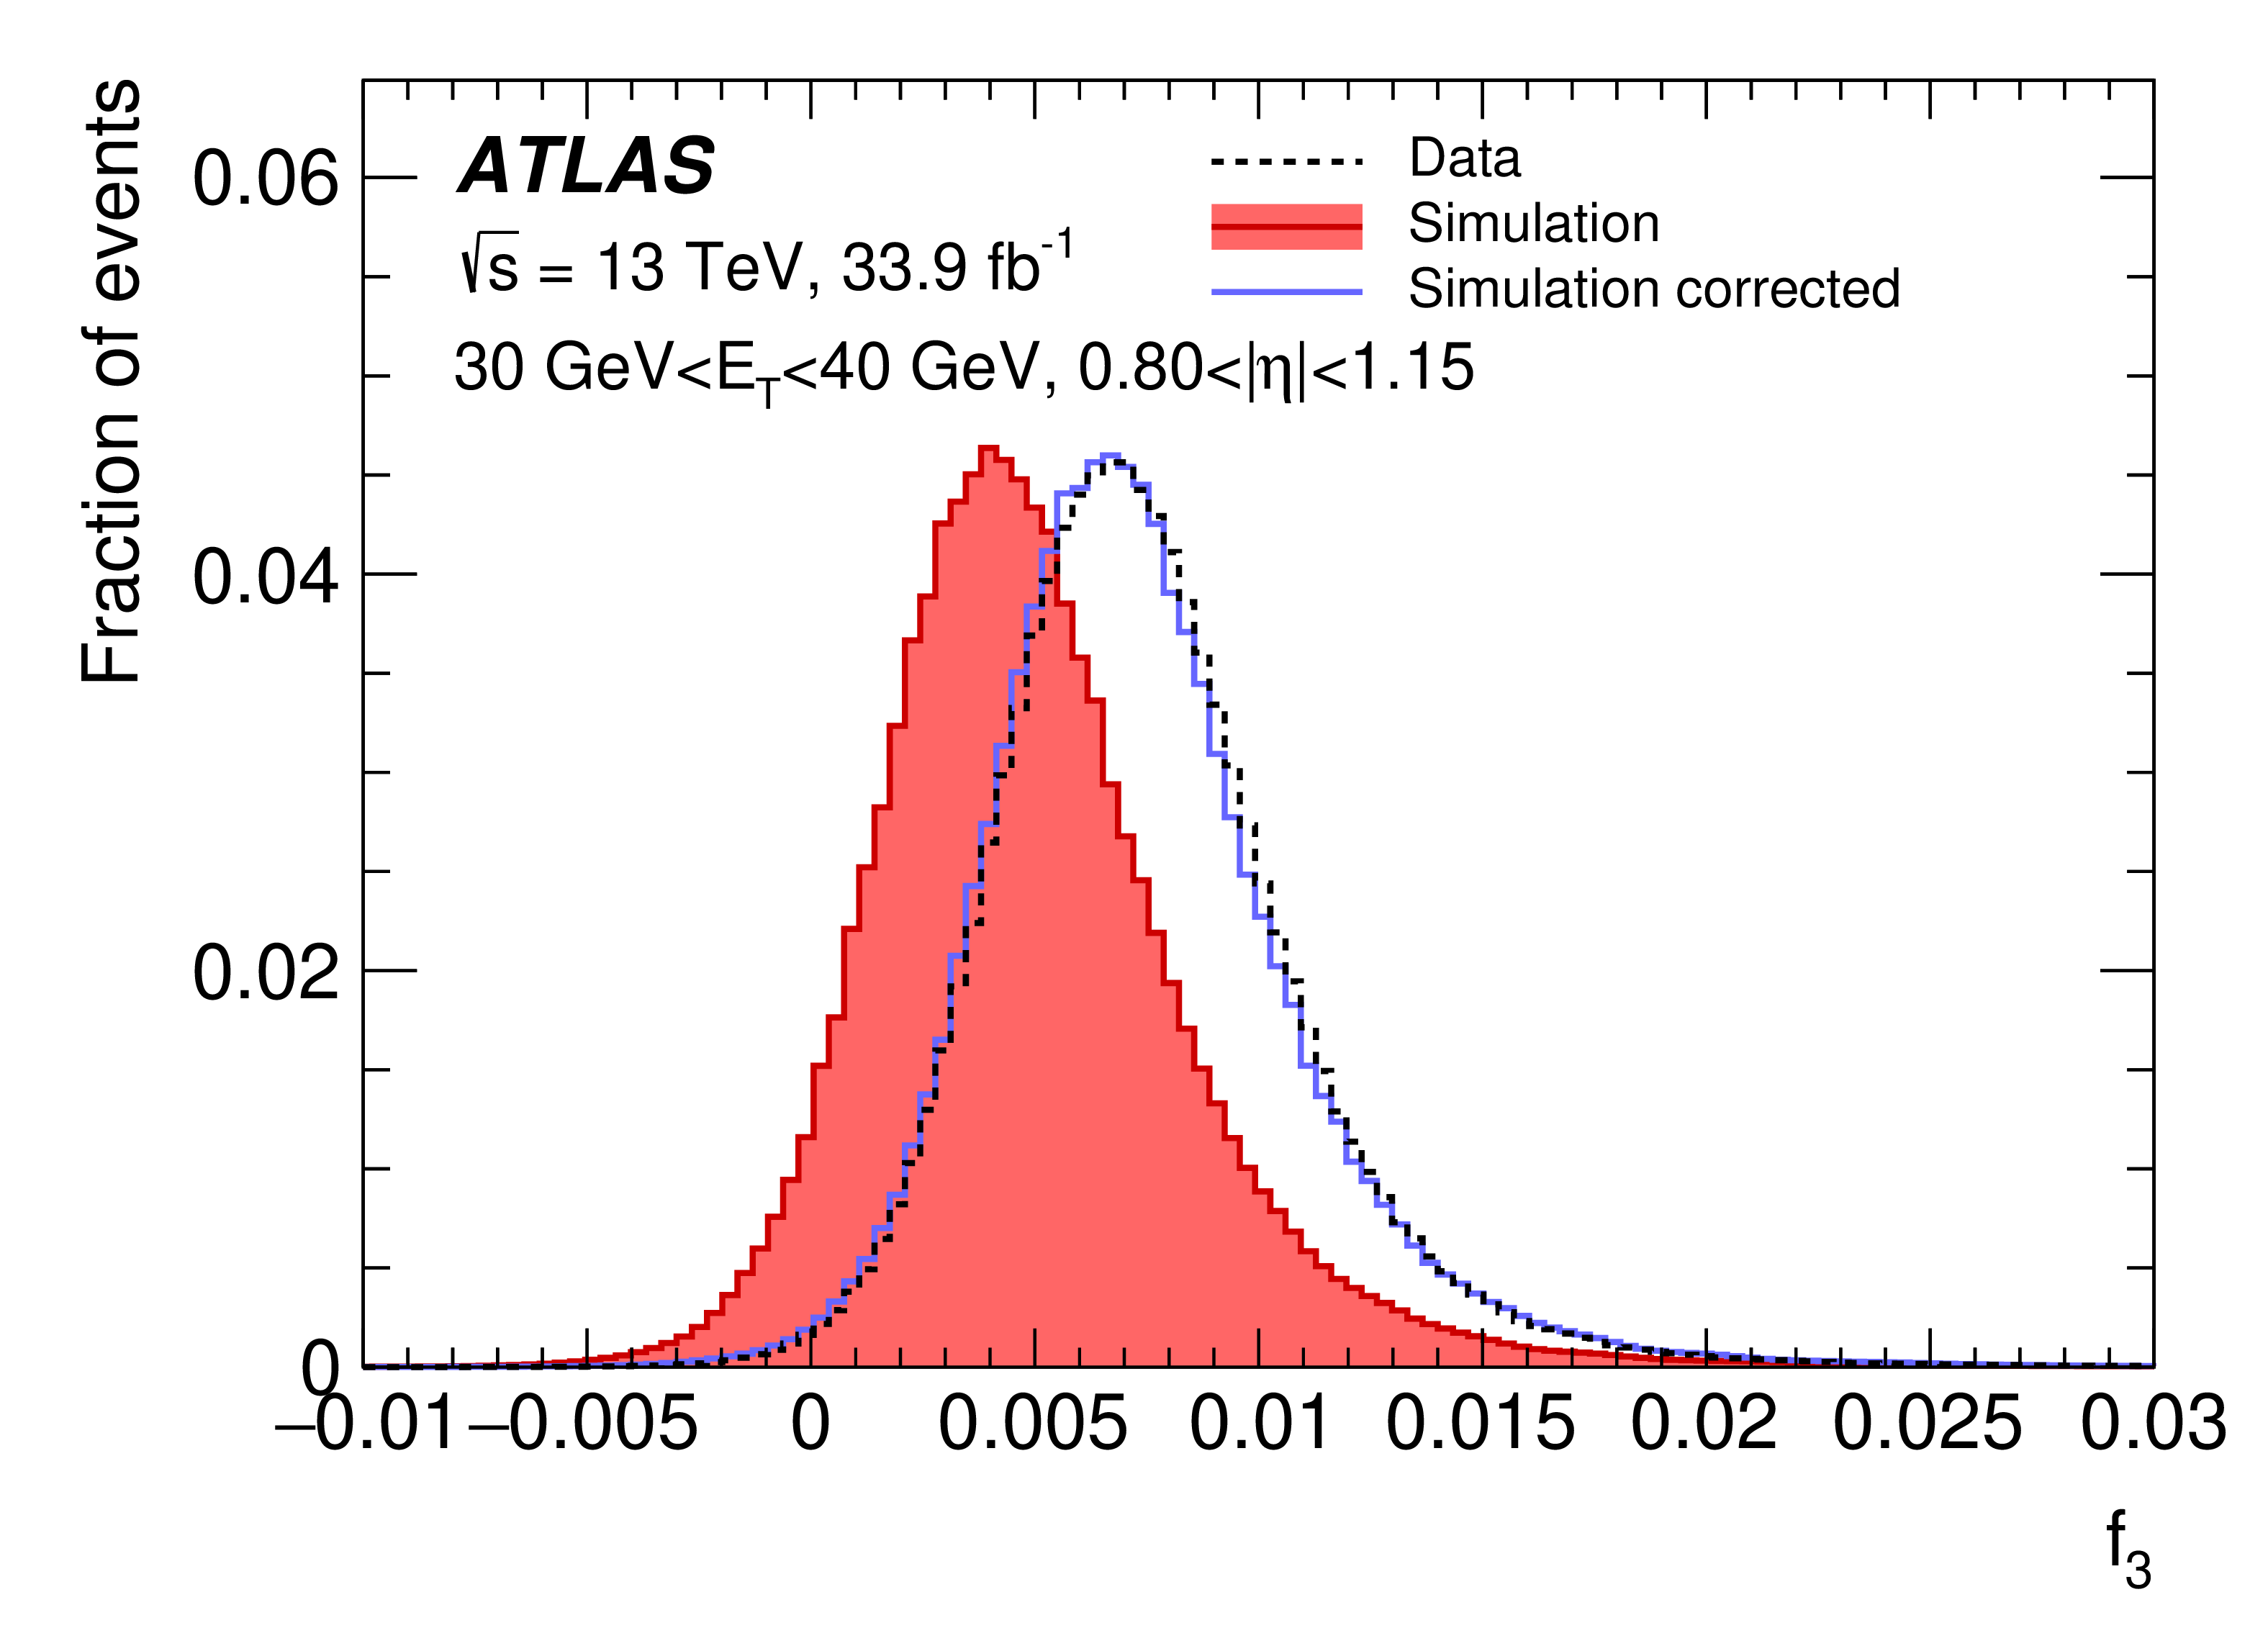
\includegraphics[width=1.00\textwidth]{figs/egamma/f3_DataVSMC.png}
\caption{}
\end{subfigure}
\hfill
\begin{subfigure}[b]{0.49\textwidth}
\centering
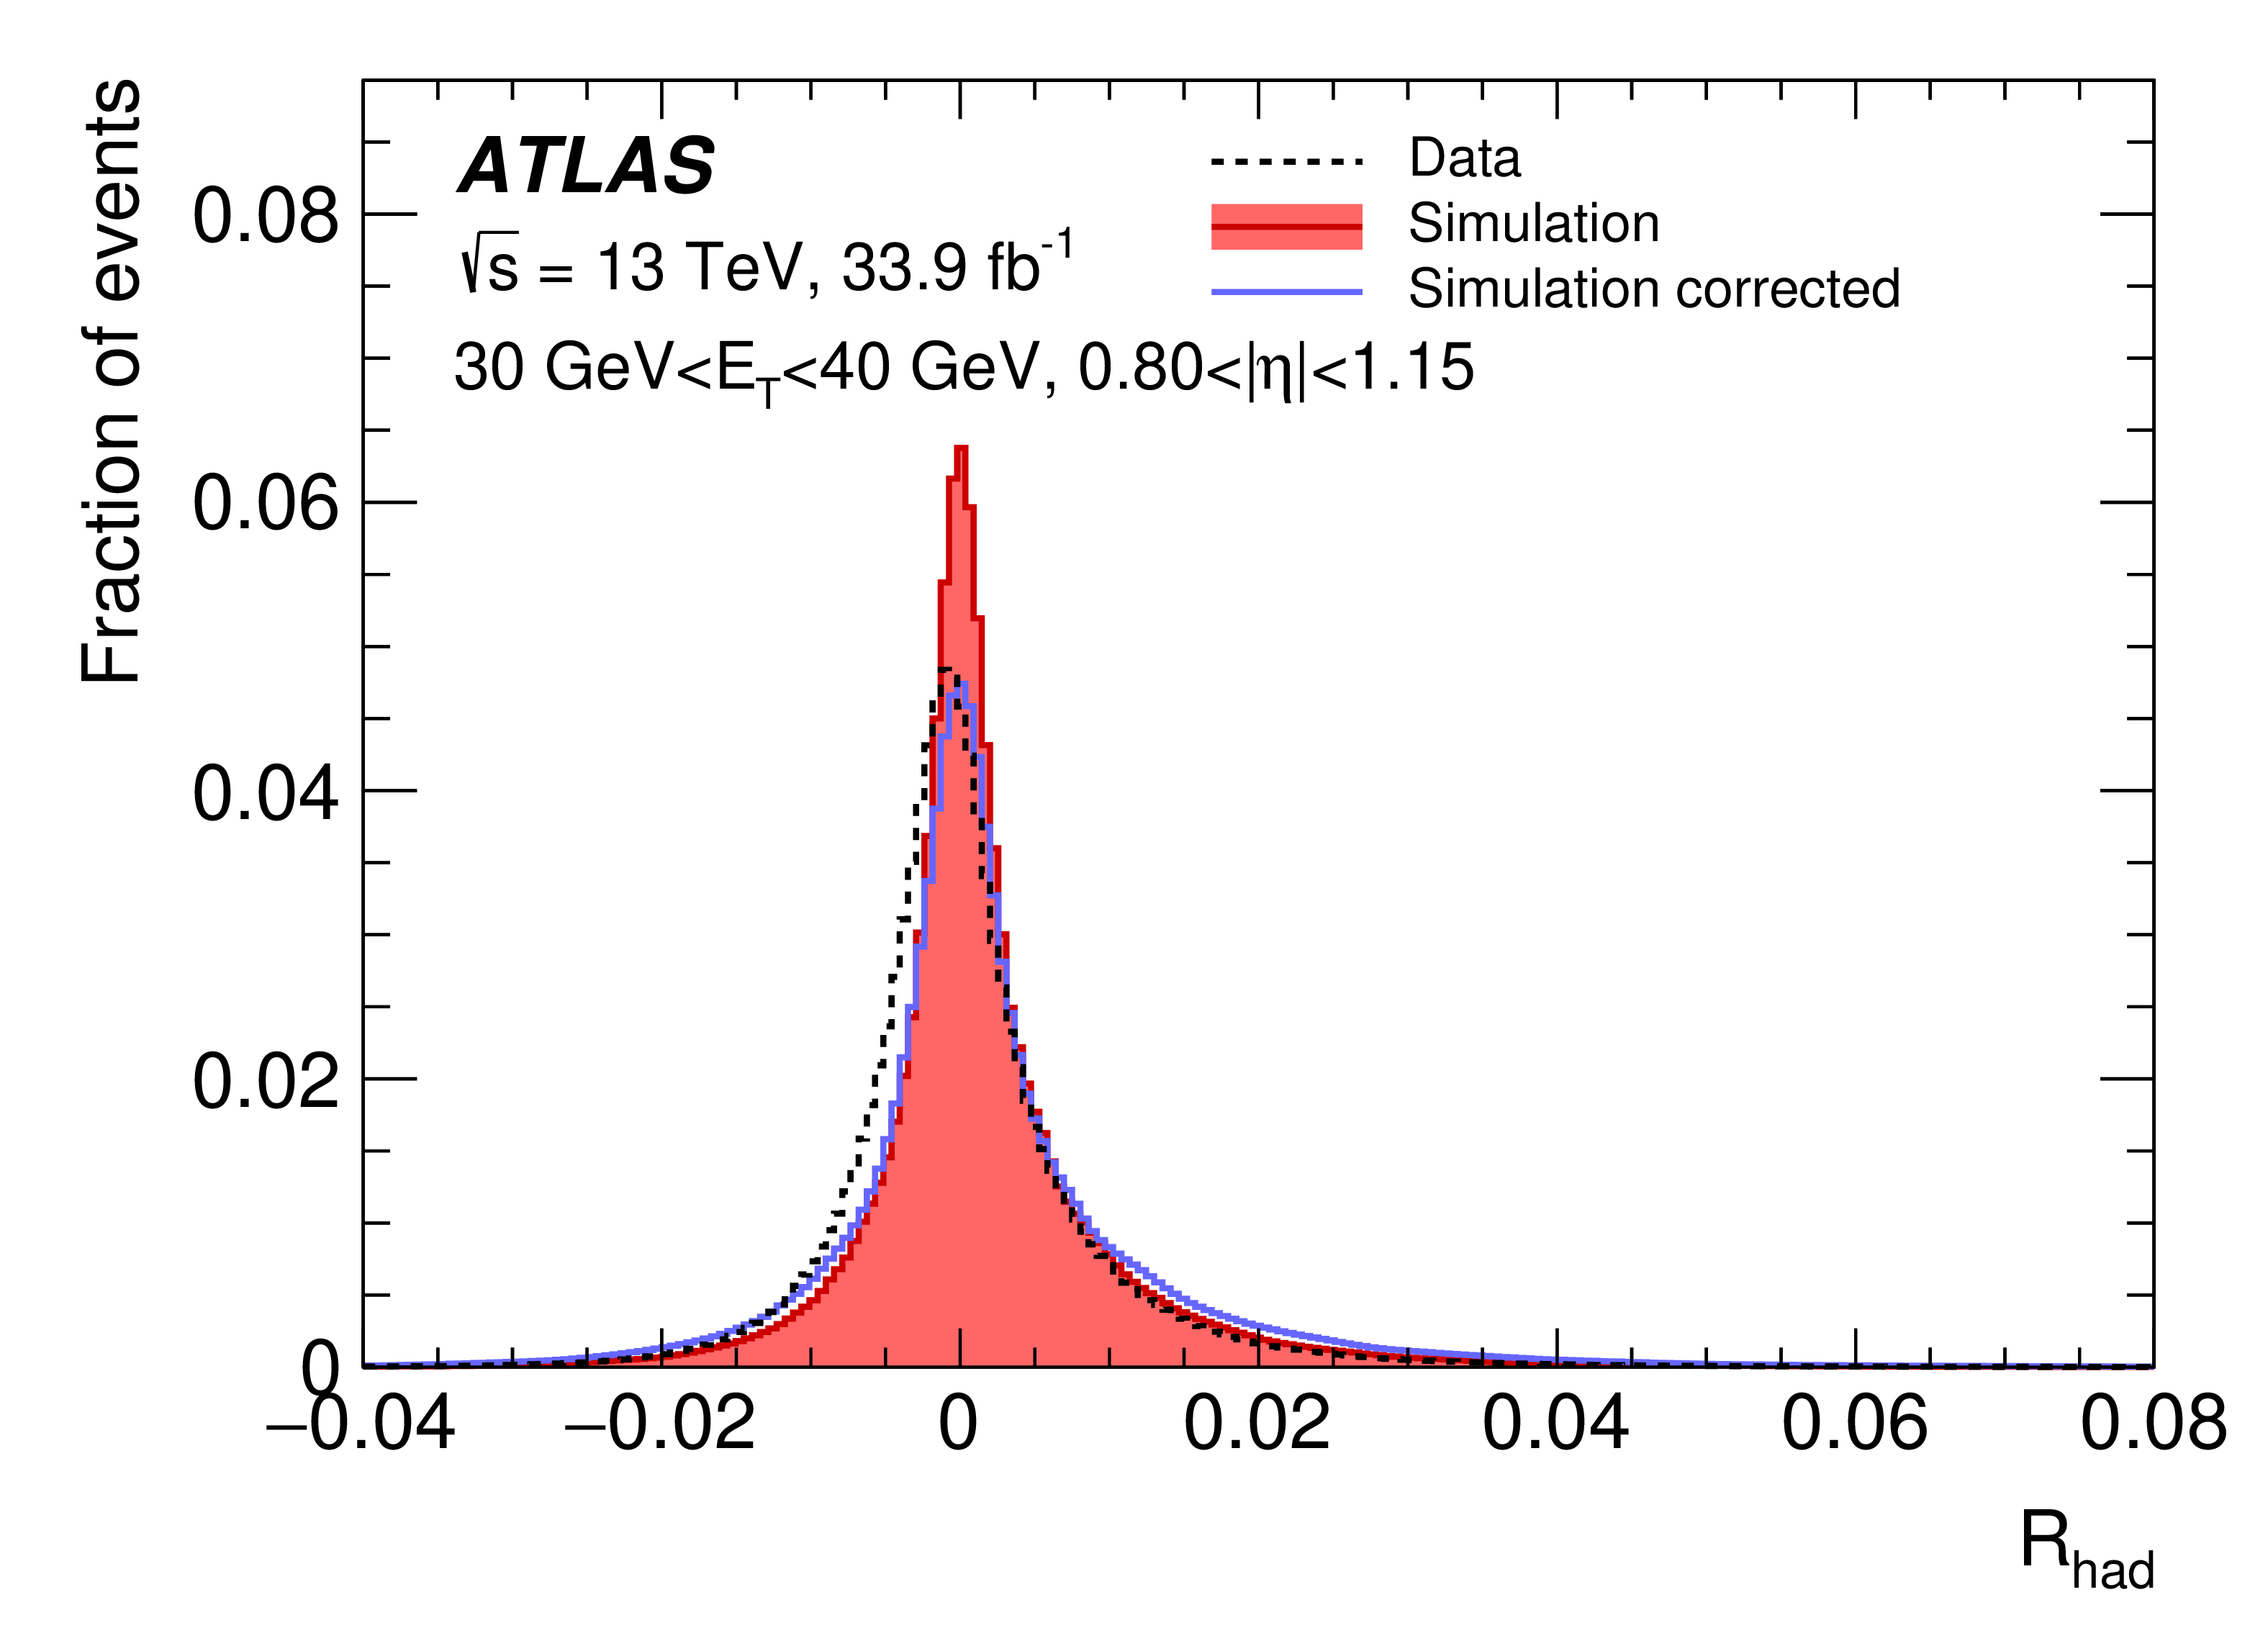
\includegraphics[width=1.00\textwidth]{figs/egamma/R_had_DataVsMC.png}
\caption{}
\end{subfigure}
\caption[Example pdfs illustrating shift and width corrections applied to MC for discriminant tuning procedure]{The \fIII (a) and \rhad (b)
  pdf distributions in data and simulation for prompt electrons that satisfy 30~\GeV $<$ \et $<$ 40~\GeV and $0.80 < \left|\eta\right| < 1.15$.
  The distributions for both simulation and data are obtained using the \Zee\ \tnp method.
  KDE smoothing has been applied to all distributions.
  The simulation is shown before (shaded histogram) and after (open histogram) applying a constant shift (\fIII, (a)) and a width-scaling factor (\rhad, (b)). 
  Although some $\left|\eta\right|$ bins of \fIII additionally
  have a width-scaling factor, this particular $\left|\eta\right|$ bin only has a constant shift applied.
}
\label{fig:egamma:data_MC_comparison_shifts}
\end{figure}

For a flat efficiency the procedure is fairly straight forward.
A large MC sample of reco level electron objects are fed into the Electron LH in order to populate a discriminant distribution for a given bin, a discriminant cut value is then chosen such that a desired selection efficiency is achieved.
This procedure becomes more nuanced when the discriminant loosening parameter, $a$, detailed in the previous section must be determined as well.
For this case a two dimensional histogram in discriminant vs. \nvtx\ is populated and bin by bin in \nvtx\ the discriminant value most closely resulting in the desired efficiency is determined.
These equi-efficiency discriminant values are then fit to a line to determine the slope, $a$.
This is illustrated in Figure \ref{fig:egamma:equiEfficiency} with the blue points all corresponding to the desired efficiency and the black line the linear fit of those points.
Now as illustrated in Figure \ref{fig:egamma:nvtxDepSignal} by the black markers the desired flat efficiency is achieved as a function of \nvtx\ as desired, however as discussed in the previous section this leads to a large \nvtx\ dependence in the background efficiency as seen in Figure \ref{fig:egamma:nvtxDepBackground}.
This see-saw effect is then countered by by-hand iterations of reducing the slope $a$ such that a relatively flat signal efficiency is retained while also ameliorating the strong \nvtx\ dependence in background, this is illustrated by the red markers in Figure \ref{fig:egamma:nvtxDep}.


\subsection{LH-identification Operating Points}
%and their corresponding efficiencies}
As different ATLAS physics analyses desire different levels of electron signal efficiency and background rejection, several operating points are necessary.
There are four levels of officially maintained and recommended \tune\textrm{s} designed to encompass a broad variety of analyses.
These are the aforementioned \VeryLoose, \Loose, \Medium, and \Tight\ operating points.
%Four operating points are defined: \VeryLoose, \Loose, \Medium, and \Tight.
Each corresponds to a more stringent requirement on the likelihood discriminant value than the one before it, and thus a larger background rejection (and correspondingly,
a smaller signal efficiency).
In addition to requirements on the discriminant value, all of the operating points also impose requirements on simple track quantities.
\Loose, \Medium, and \Tight\ require at least two hits in the pixel detector and at least seven hits in the pixel and silicon strip detectors combined.
Furthermore, \Medium\ and \Tight\ also require a hit in the innermost pixel layer, which is useful for rejecting photon conversions.
In cases where the innermost pixel layer is non-operational, the next-to-innermost pixel layer is used instead.
A variation of the \Loose\ operating point called \LooseAndBLayer\ also exists, which uses the same criteria as Loose but also adds the requirement of a hit in the innermost pixel layer.
The \VeryLoose\ operating point primarily exists for fake electron background estimation, and thus only requires a ``good-quality'' track, which is defined as at least one hit in the pixel detector (which need not be a hit in the innermost pixel layer) and at least seven hits in the pixel and silicon strip detectors combined.
%The efficiencies of these electron identification operating points in simulated \Zee, \Jee, and dijet samples are shown in Figure~\ref{}. 

\subsection{The Trigger Electron LH} \label{sec:egamma:trigger}
%\textcolor{red}{\hrulefill \textsc{Unfinished Section. Still need to add my specific contributions}\hrulefill}\\
The time between a collision and the final ATLAS trigger decision is about 4 seconds.
In order to to meet this time requirement trigger reconstruction algorithms that are CPU-intensive must be altered with respect to their offline equivalents.
In the case of the electron/photon reconstruction and identification algorithms this affects several inputs and techniques nominally used offline.
The variable-sized supercluster algorithm described in Section \ref{sec:egamma:supercluster} was not used online in Run-2.
Neither is the GSF electron track refitting where instead the standard pion hypothesis track fitting must be used.
As a result the quality of the track reconstruction degrades, impacting the resolution of the $d_{0}$ and \dOSignificance\ tracking variables, as as well as the trackcluster matching variables \deltaphires\ and \deltaeta. %offical figure needed here
The variable \deltapoverp\, which is output by the GSF algorithm, is unavailable altogether at the HLT.
During the reconstruction of electromagnetic clusters in the LAr calorimeter, some cell-energy-level corrections are not available online, such as the correction for transient changes in LAr high-voltage~\cite{LARG-2009-01}, or differ in implementation, such as the bunch crossing position-dependent pileup correction~\cite{ATL-DAQ-PUB-2017-001, PERF-2017-03, Aad:2019wsl}.

%The availability of pileup measure information is also limited online.
%Full event reconstruction is required to determine the number of primary vertices; this variable, which is used offline to correct for the electron LH's pileup dependence (detailed in Section \ref{sec:egamma:pileup}), must be substituted at the HLT with a different variable.
%The reasonable replacement is the average number of collision vertices $\langle \mu \rangle$, measured online by a set of luminosity detectors (one dedicated detector LUCID, the Beam Conditions Monitor, and measurements from the Tile and Forward calorimeters and the ID.
%While the actual number of interactions in a bunch crossing fluctuates, and can depend on the location of the colliding bunch in the bunch train, the $\langle \mu \rangle$ is the average over all BCIDs in a lumiblock (one minute of data taking) and acts as a reasonable proxy for the in-time and out-of-time activity in the detector.

\subsubsection{Re-tuning the Trigger LH for Large Pileup Environments}
Re-tuning the LH is desired when a change in data taking conditions could adversely effect the performance of the LH.
In late 2017 during the historically high pileup runs it became urgent to re-optimize many recommendations as the $\mu$ for 2018 could be just as large (and potentially even larger).
For reference listed below are is fill scheme for the middle part of 2017 data taking and it's resulting peak $\mu$, as well as what the potential beam fill schemes for 2018 could be at the time (October 2017) and their expected maximum $\mu$:
\begin{itemize}
    \item 2017: 1.53$\times 10^{34}$ with 1860 bunches $\rightarrow$ $\mu$=58
    \item 2018: 2.0$\times 10^{34}$ with 2550 bunches $\rightarrow$ $\mu$=56 
    \item 2018: 2.2$\times 10^{34}$ \footnote{2.2$\times 10^{34}$ is LHC's ``limit'' – cooling of inner triplets} with 2550 bunches $\rightarrow$ $\mu$=61
    \item 2018 (8b4e): 2.2$\times 10^{34}$ with 1860 bunches $\rightarrow$ $\mu$=84 (maybe even higher)
\end{itemize}
The e/$\gamma$ Trigger working sub-group requested a re-tune of the Trigger LH to account for these potential large pileup environments expected in 2018.
For this re-tune a set of official high-$\mu$ MC samples were generated with a $\mu$-profile between 45-75.
Additionally this re-tune allowed for the entire LH (both online and offline) to be completely data-driven with the implementation of low \et\ data-driven pdfs\footnote{The low-\et Trigger LH pdfs were MC based for Run 2 prior} for this \tune.
Data-driven pdfs were derived using the full 2017 data set.
These pdfs, for both signal and background, are compared to the previous set of pdfs for high and low \et\ in Figures~\ref{fig:egamma:trig_pdfs_highet} and~\ref{fig:egamma:trig_pdfs_lowet} respectively.
\begin{figure}[p]
\centering
  \begin{subfigure}[b]{0.49\textwidth}
    \centering
    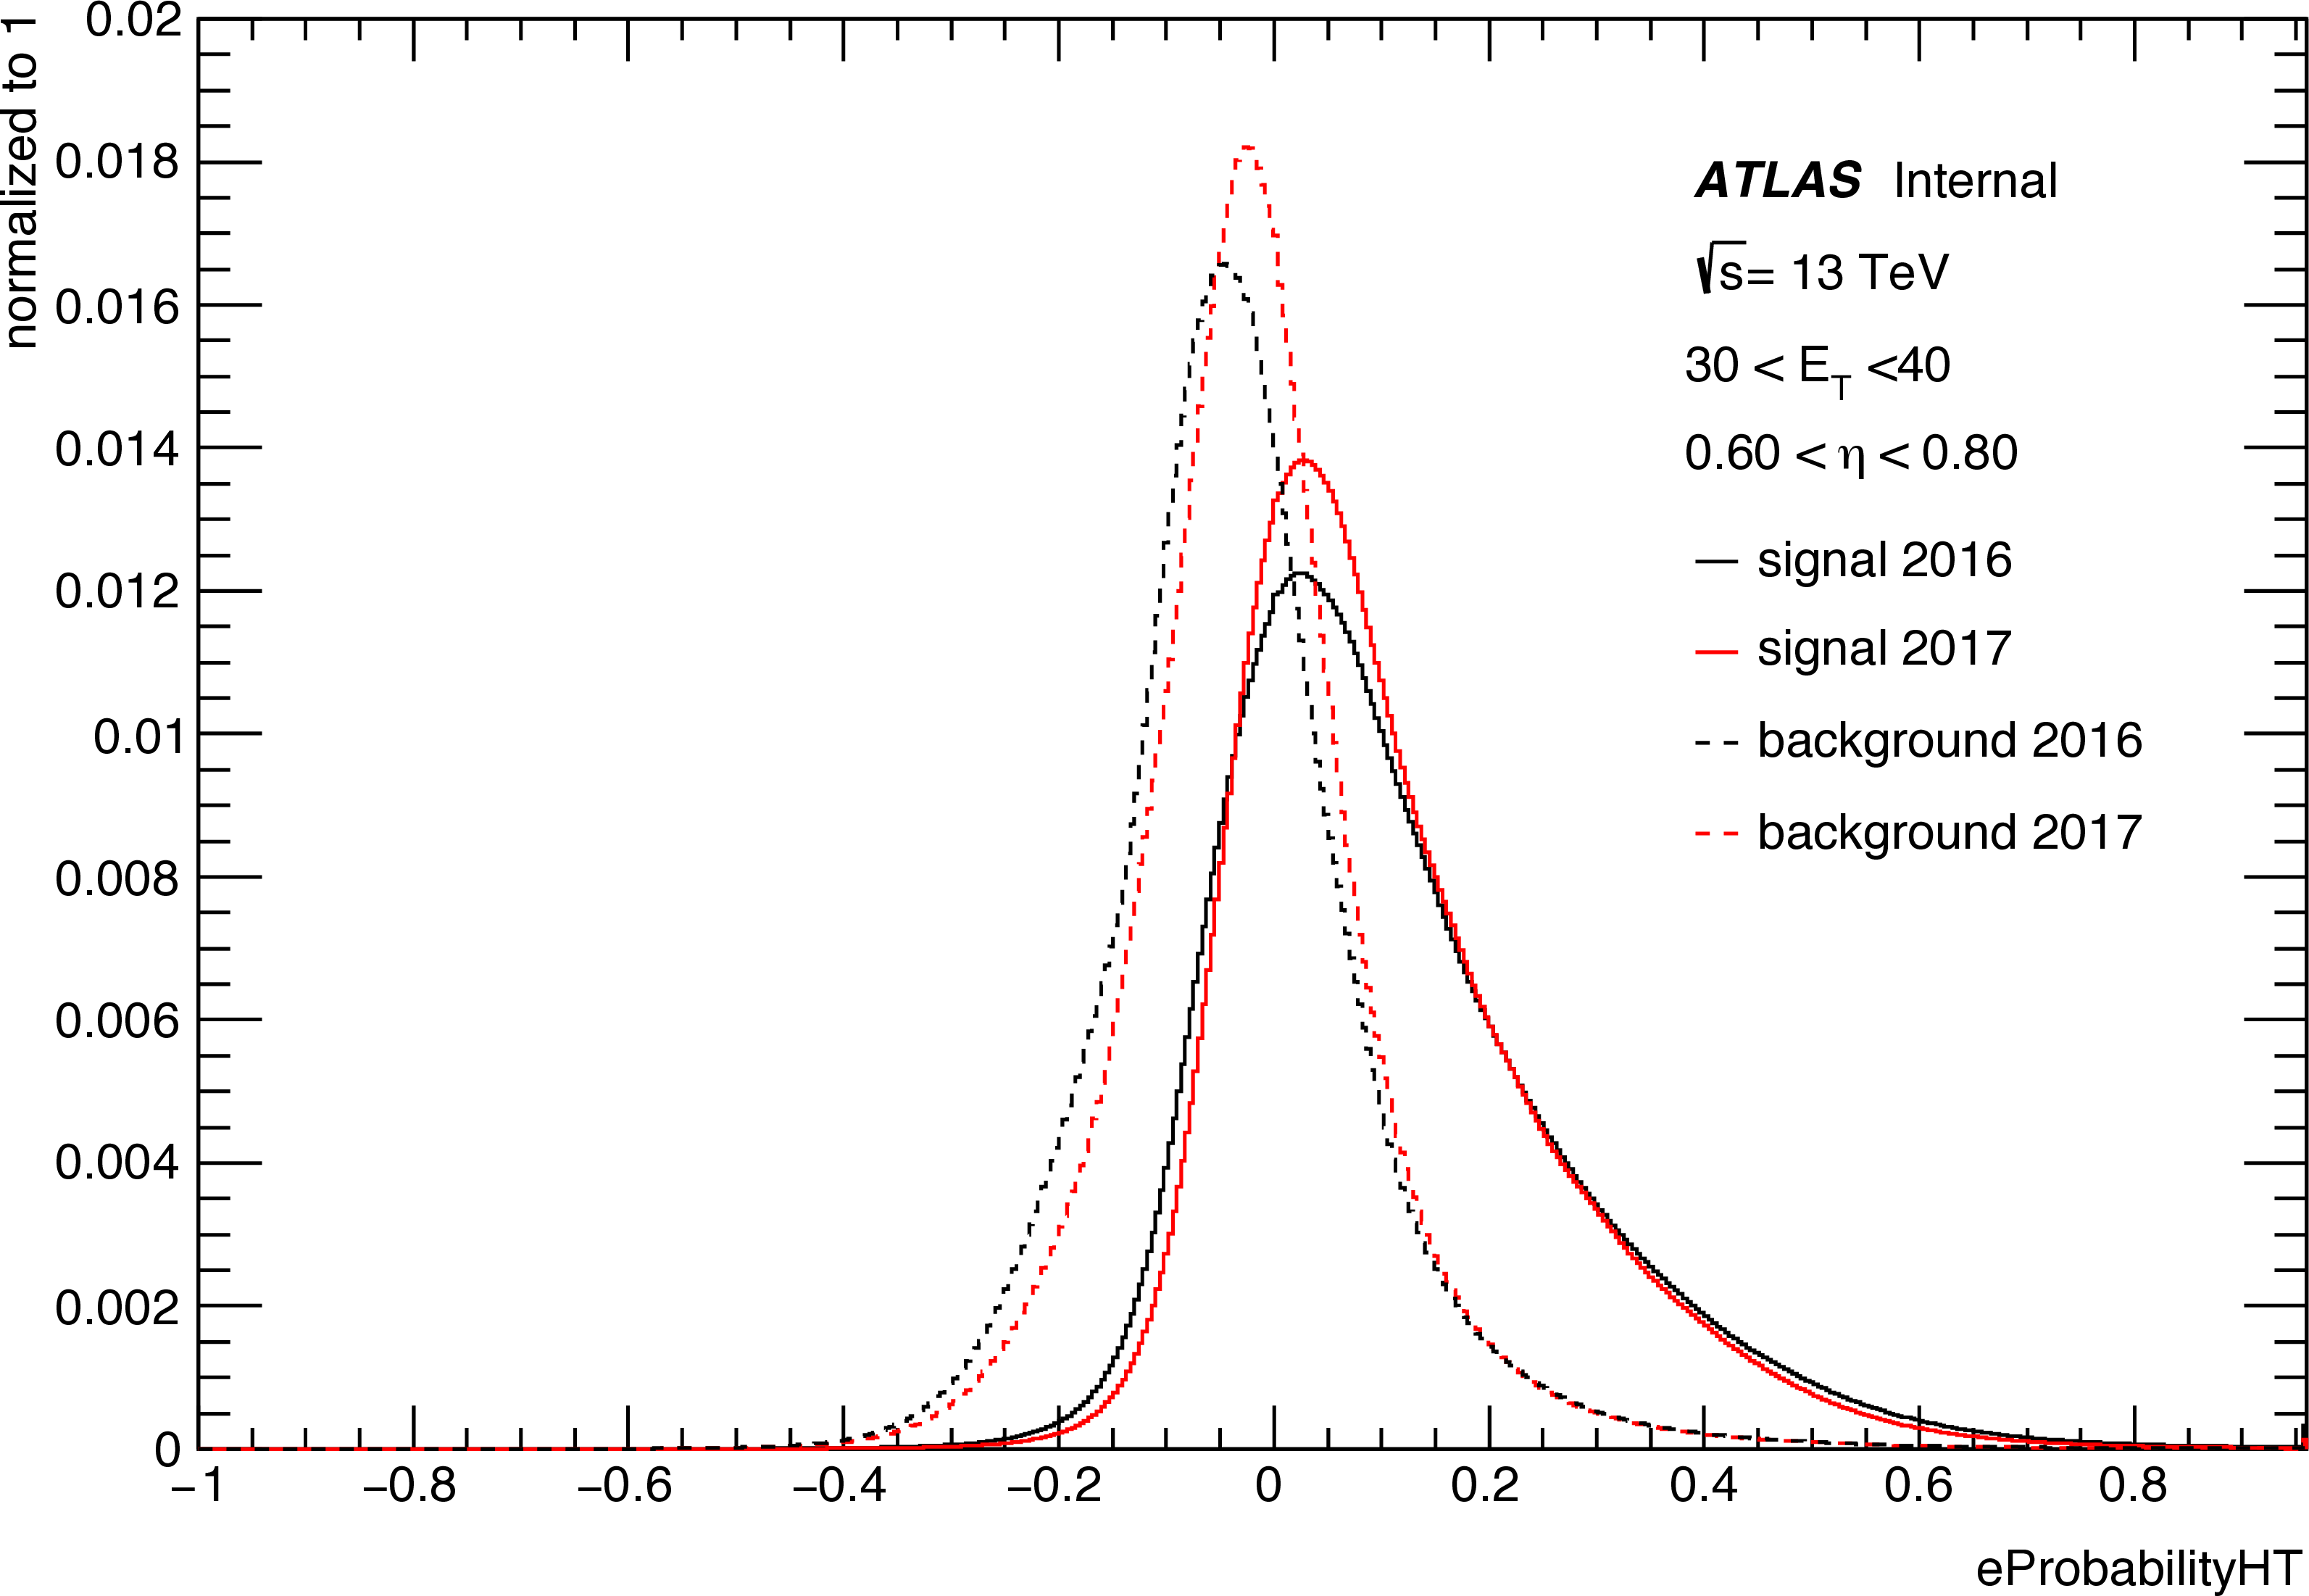
\includegraphics[width=1.0\textwidth]{figs/egamma/trig_eProb_highet.png} 
    \label{fig:egamma:trig_eProbHT}
  \end{subfigure}
  \hfill
  \begin{subfigure}[b]{0.49\textwidth}
    \centering
    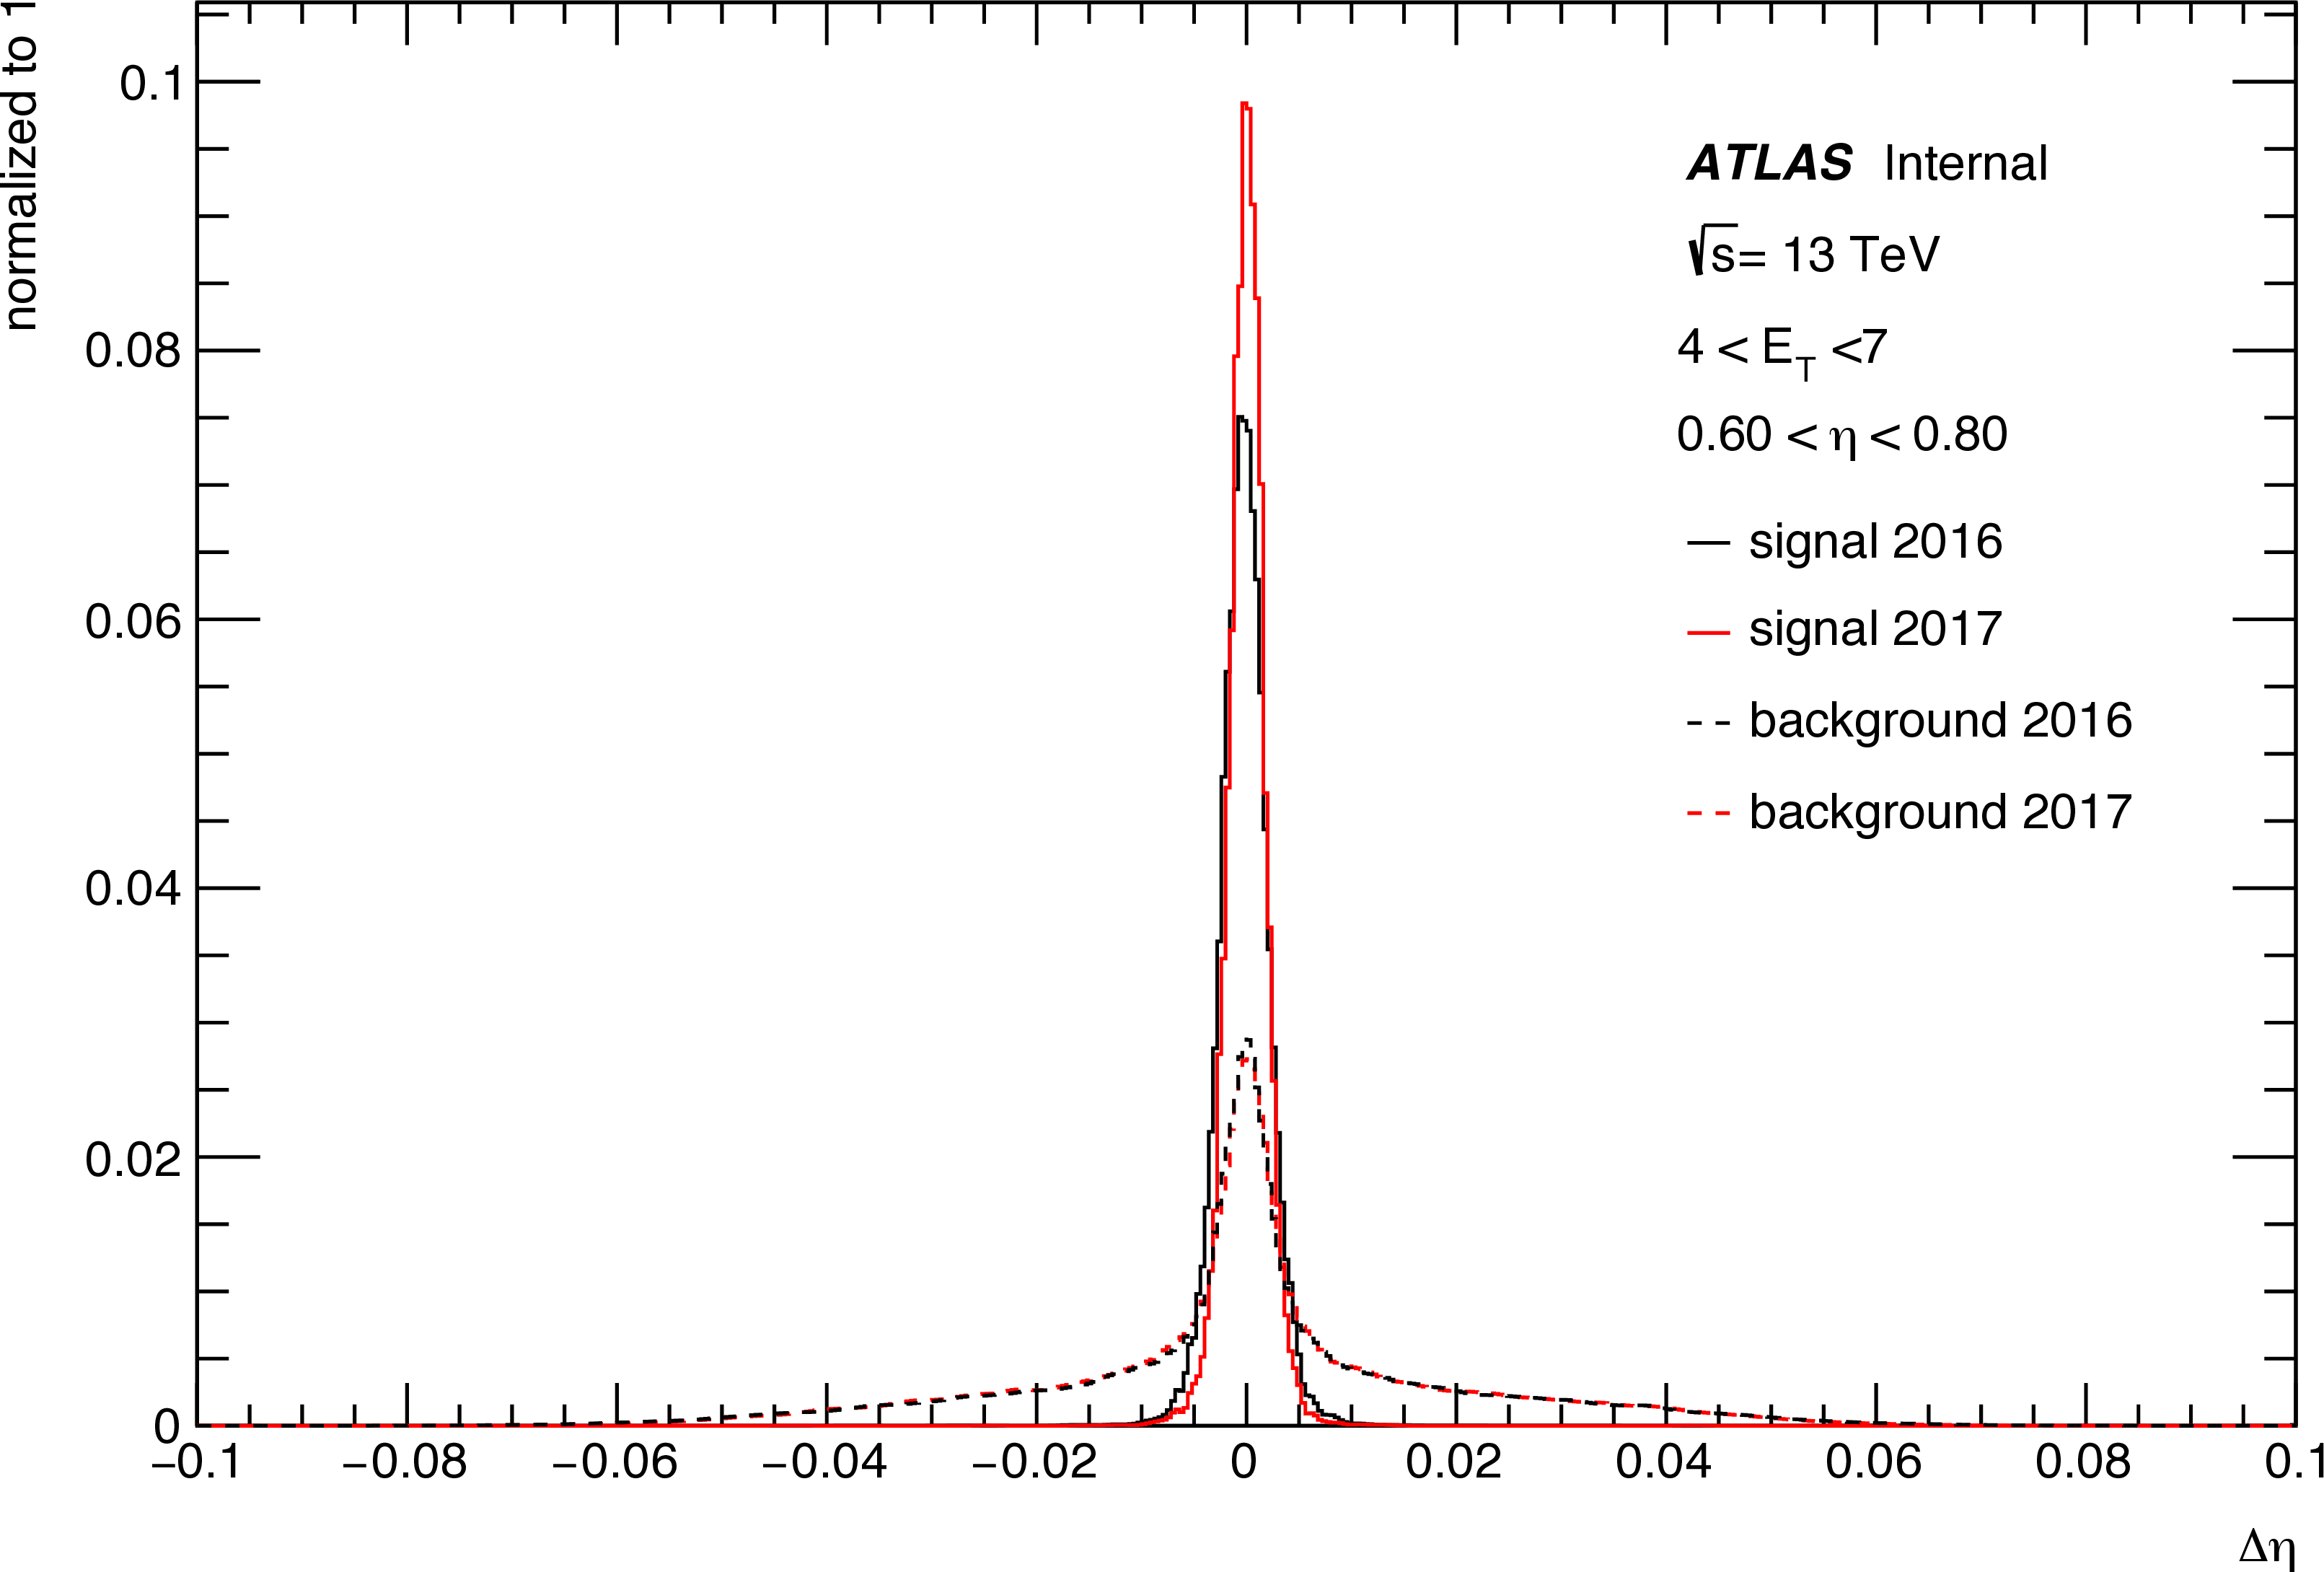
\includegraphics[width=1.0\textwidth]{figs/egamma/trig_deltaeta_highet.png} 
    \label{fig:egamma:trig_deltaEta_1}
  \end{subfigure}
  \hfill
  \begin{subfigure}[b]{0.49\textwidth}
    \centering
    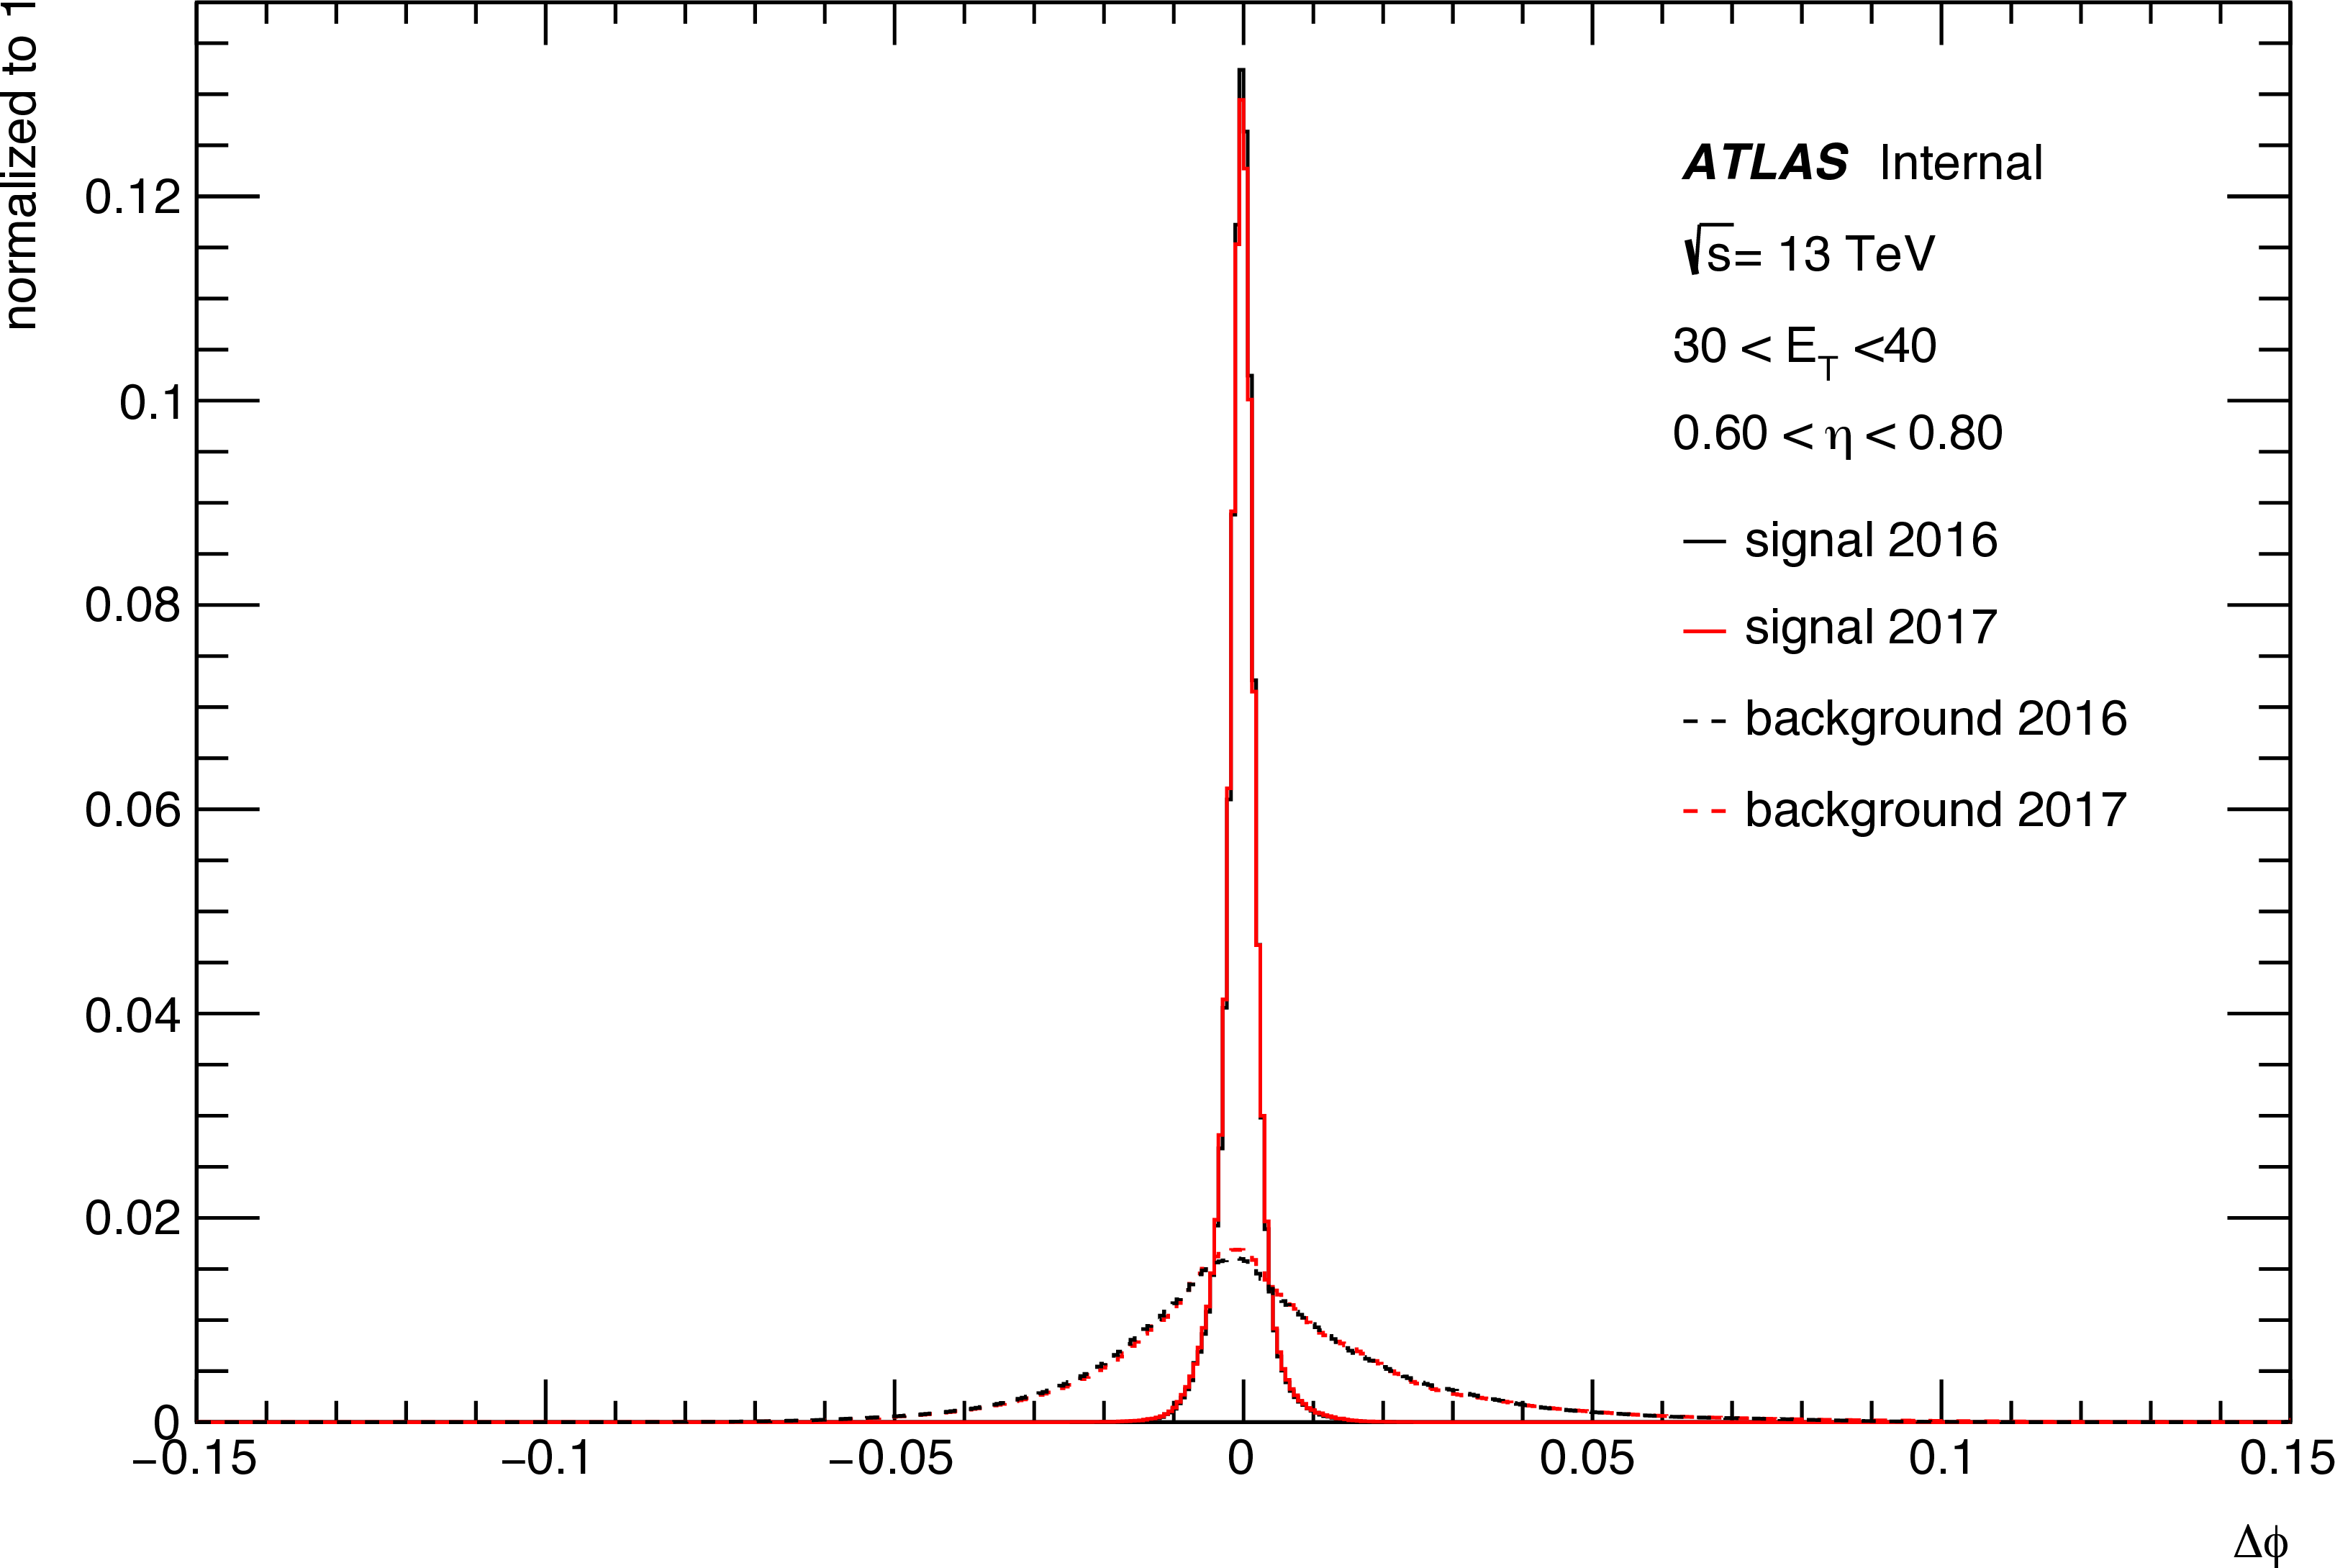
\includegraphics[width=1.0\textwidth]{figs/egamma/trig_deltaphi_highet.png} 
    \label{fig:egamma:trig_deltaPhi_res}
  \end{subfigure}
  \hfill
  \begin{subfigure}[b]{0.49\textwidth}
    \centering
    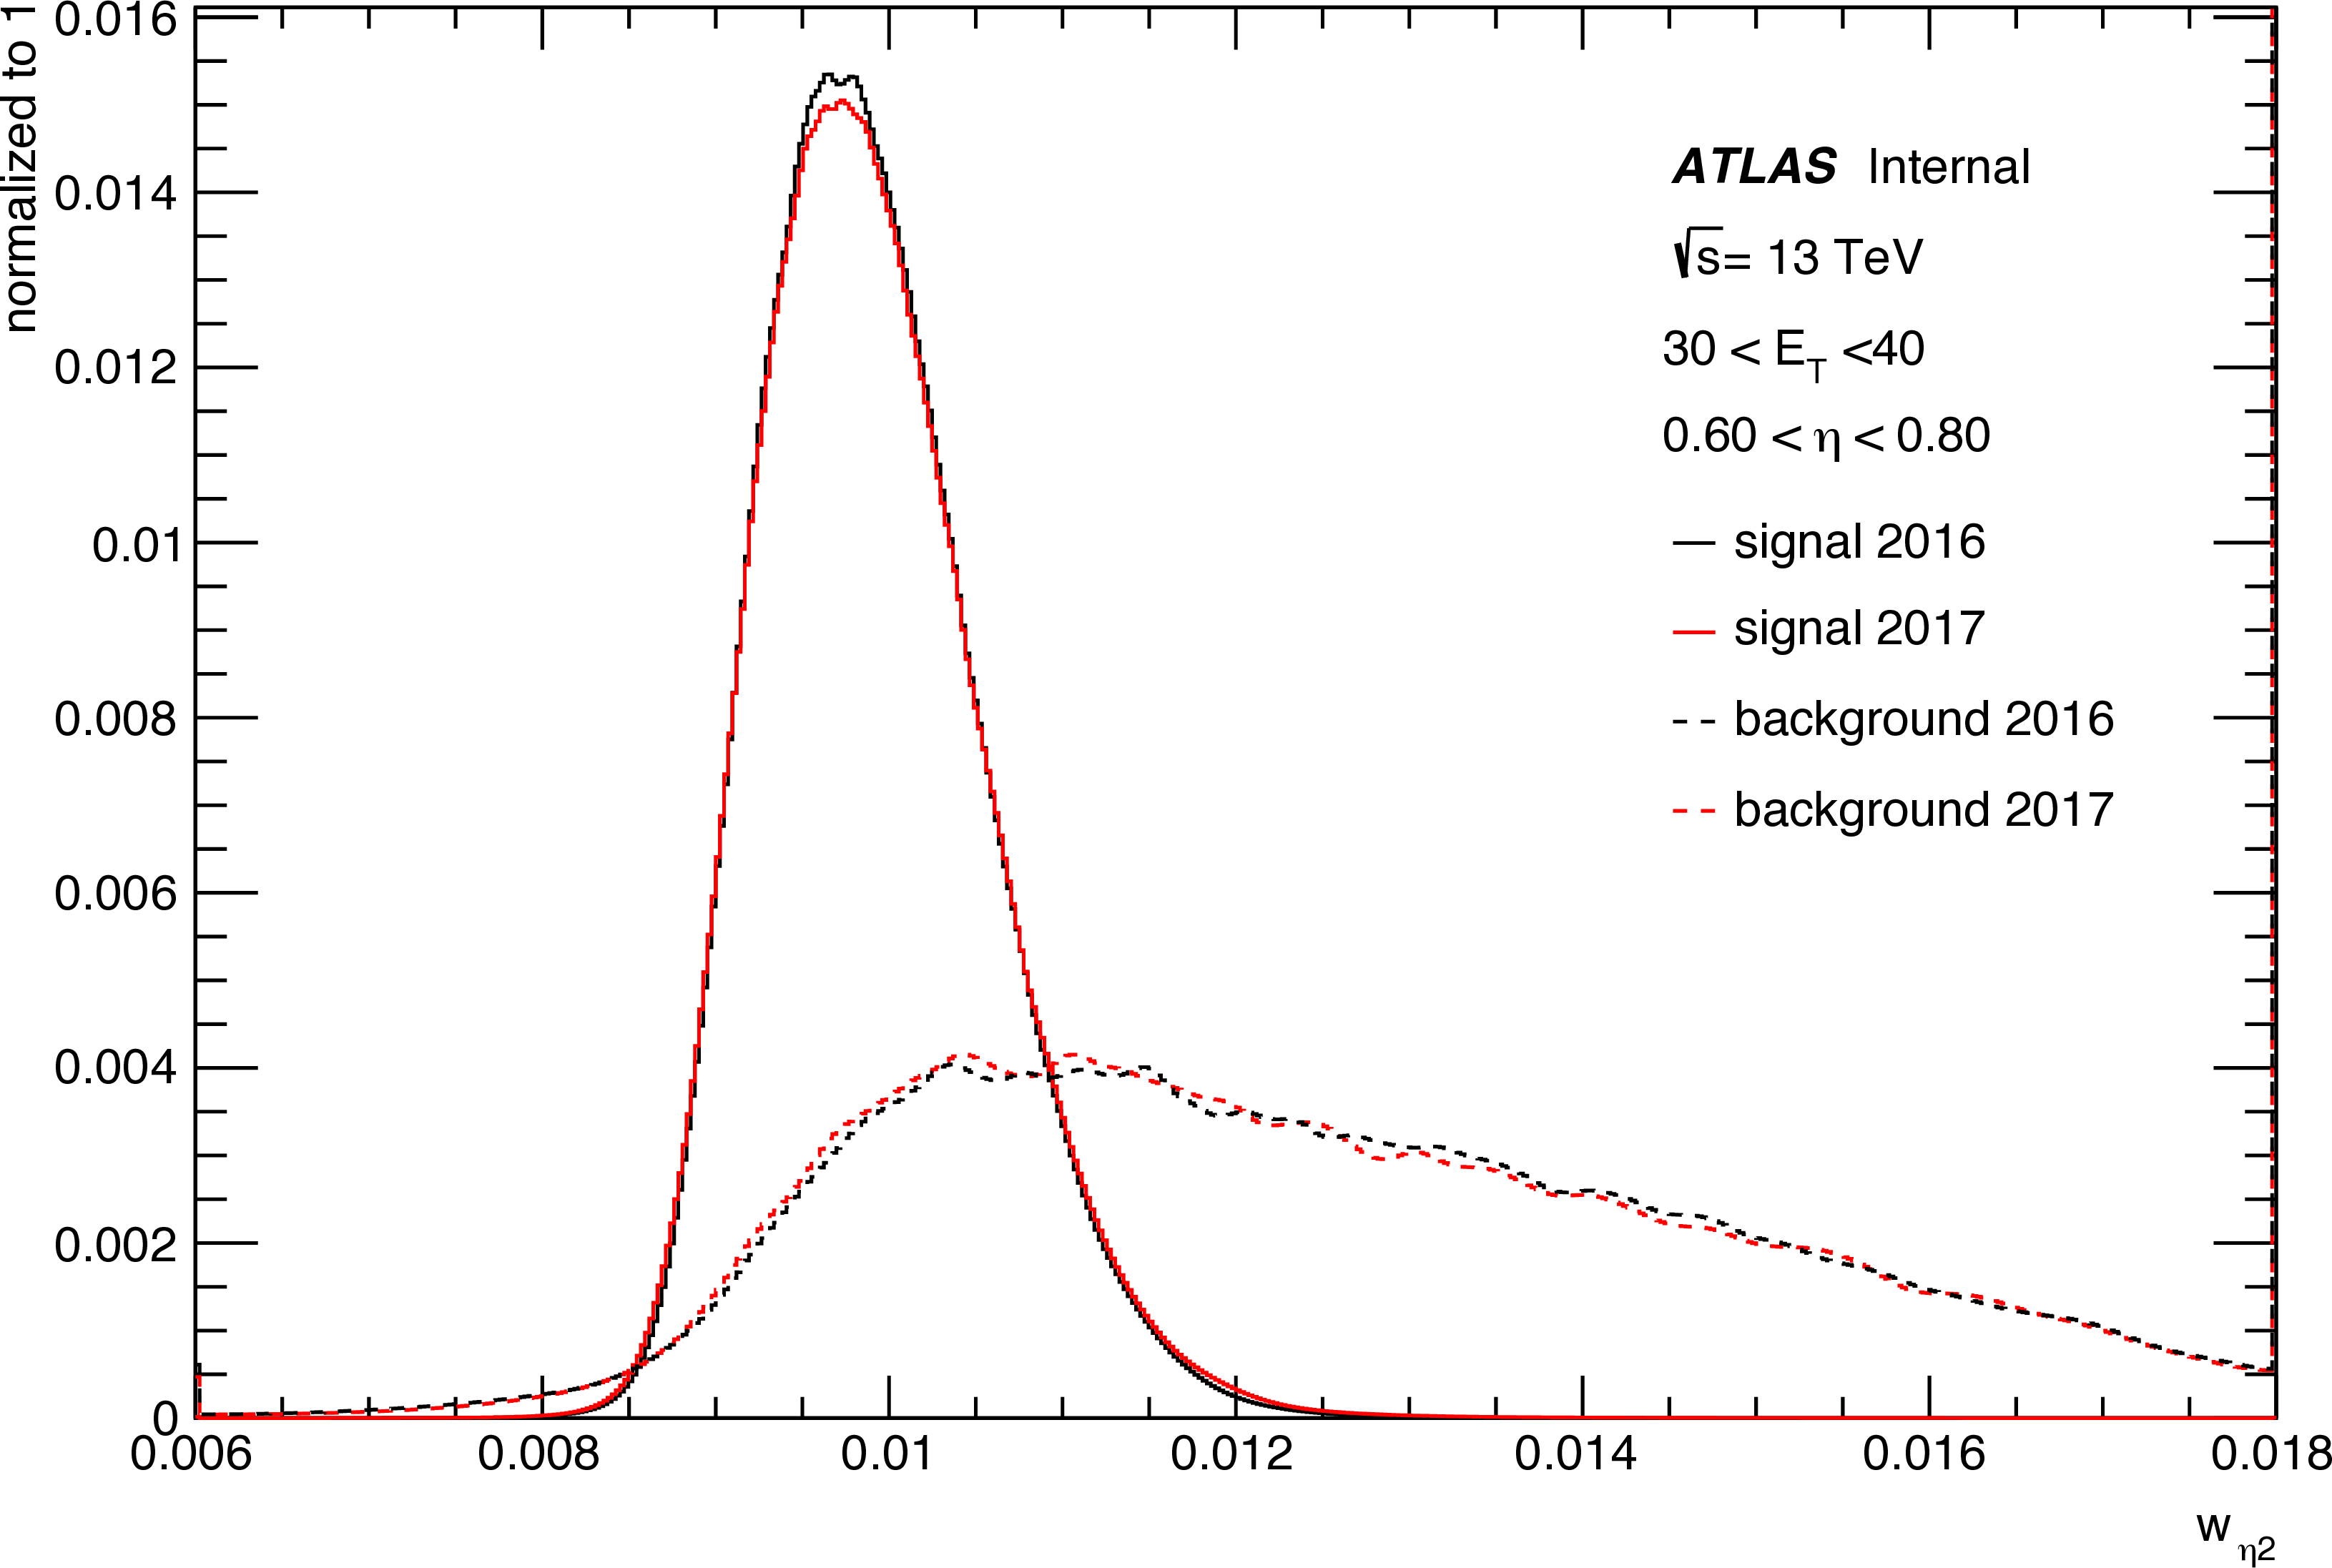
\includegraphics[width=1.0\textwidth]{figs/egamma/trig_weta2_highet.png} 
    \label{fig:egamma:trig_weta2}
  \end{subfigure}
  \begin{subfigure}[b]{0.49\textwidth}
      \centering
    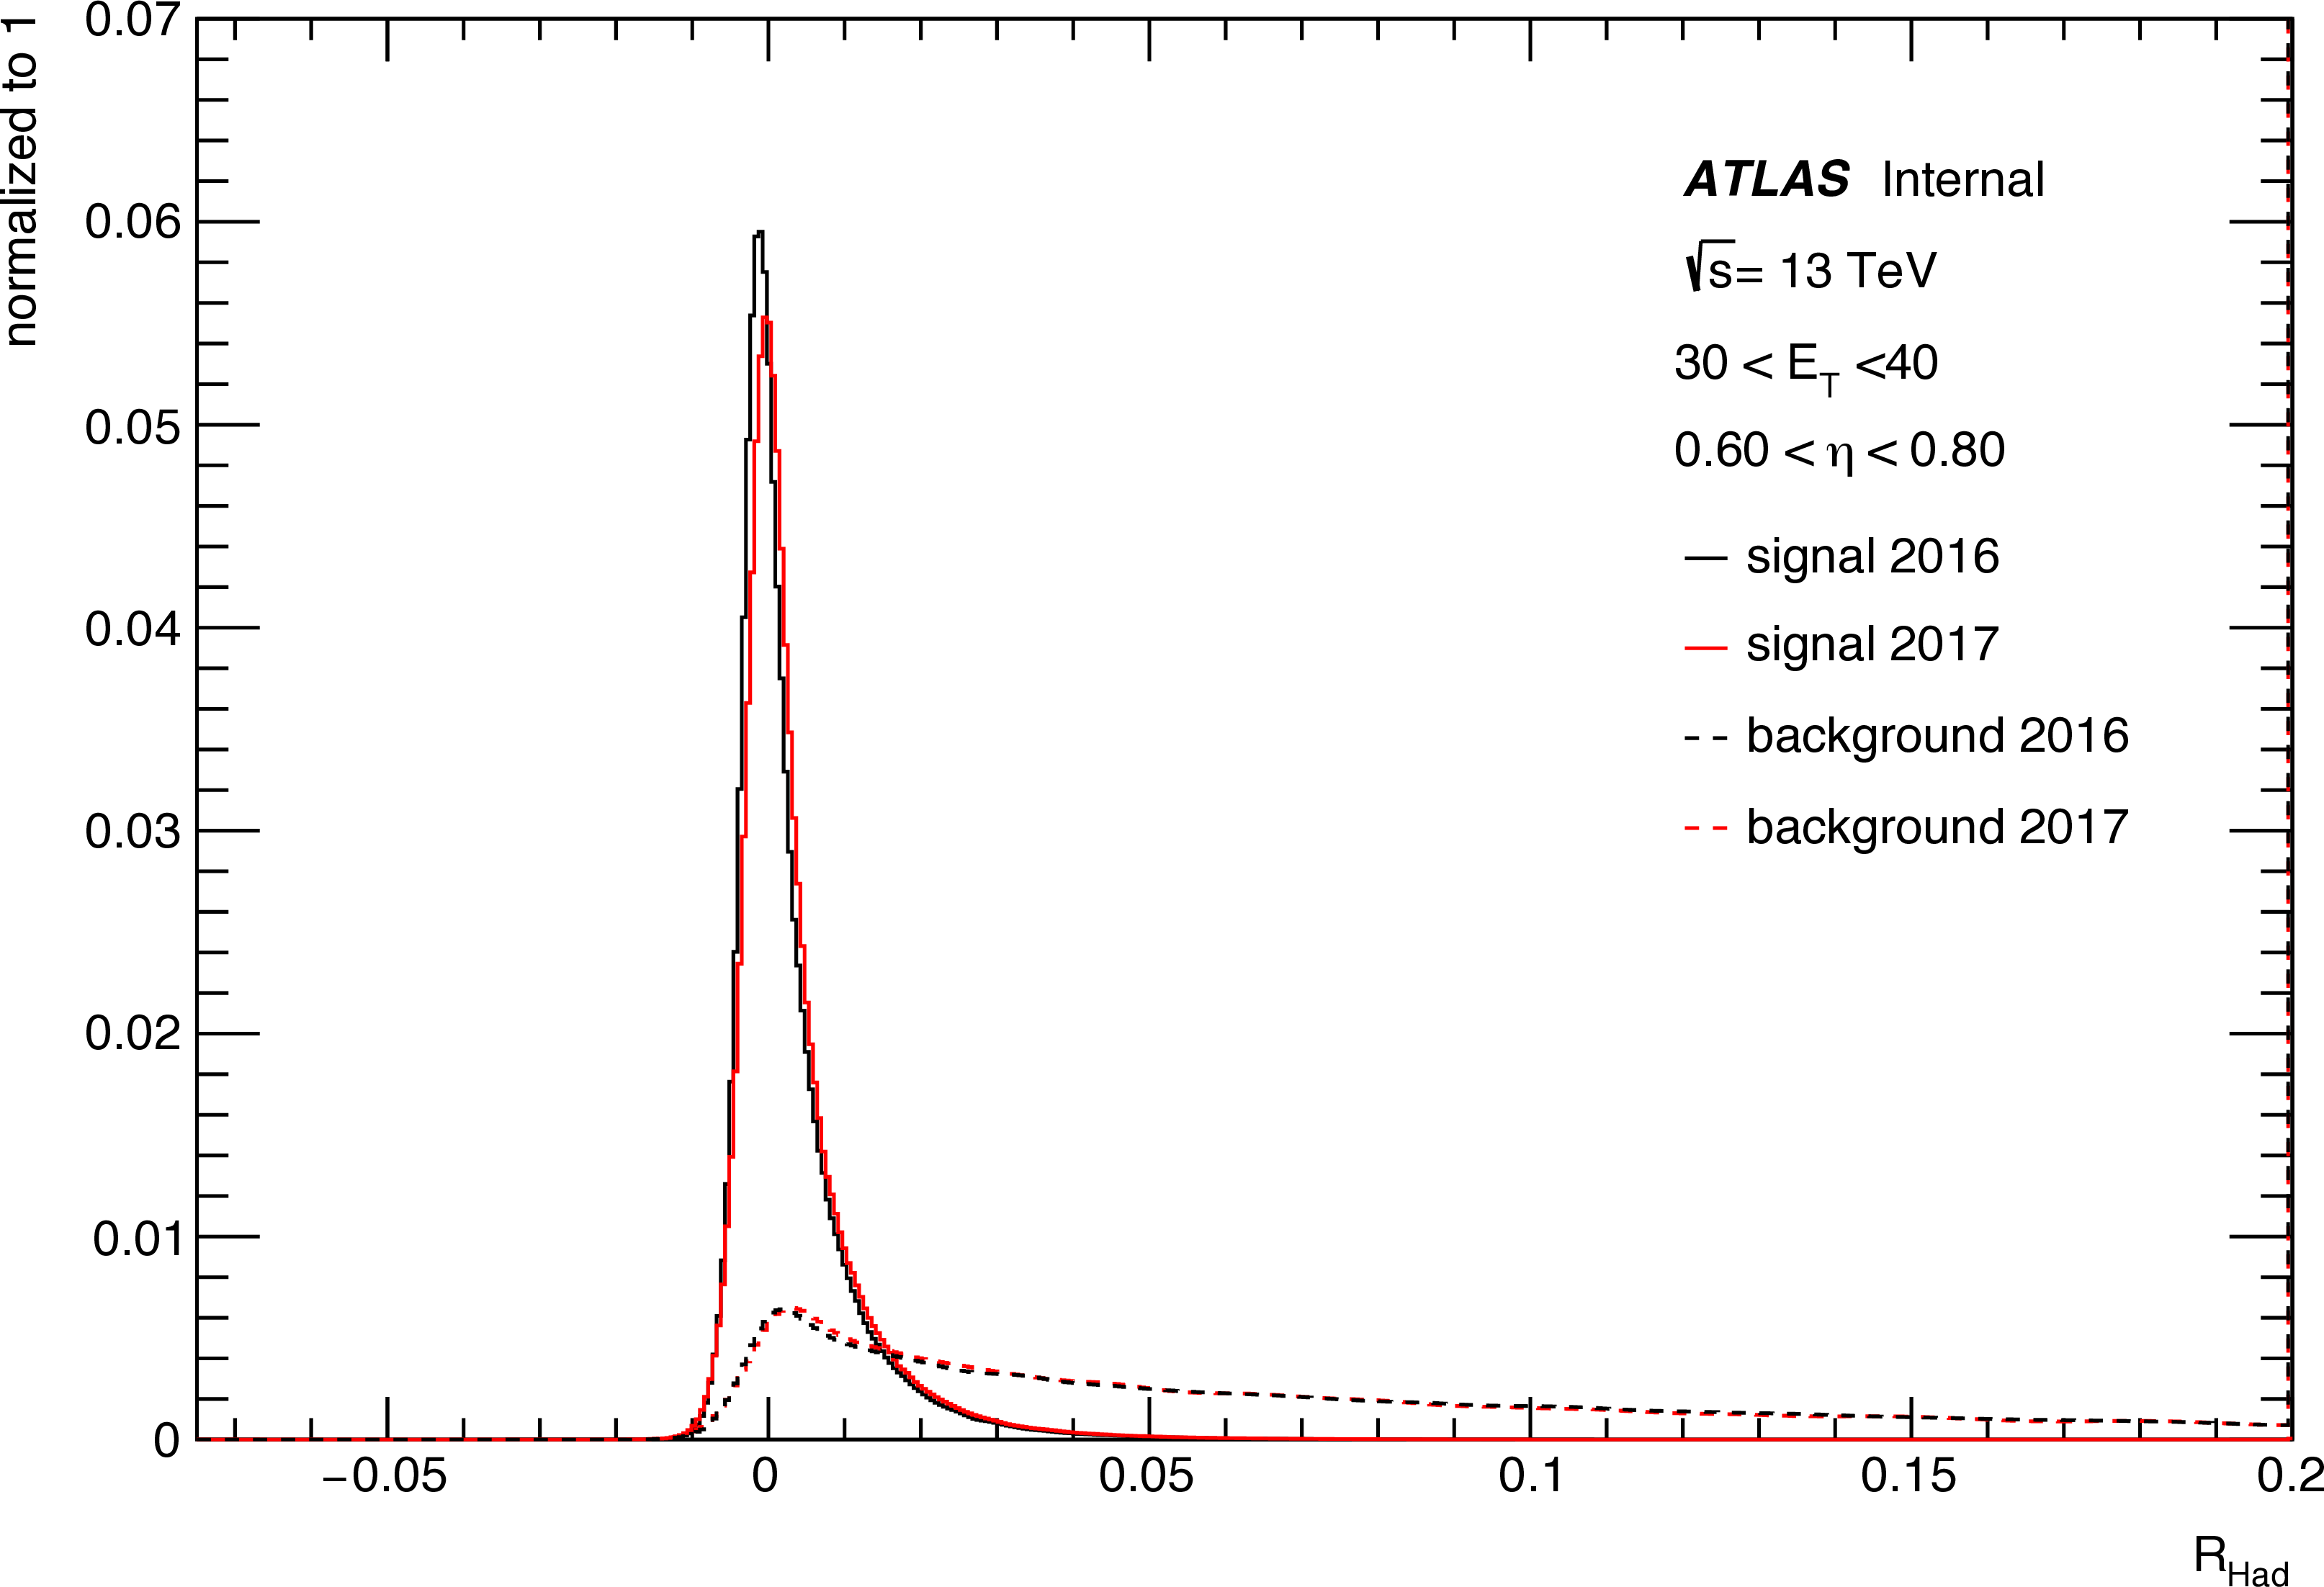
\includegraphics[width=1.0\textwidth]{figs/egamma/trig_rhad_highet.png} 
    \label{fig:egamma:trig_rhad}
  \end{subfigure}
  \hfill
  \begin{subfigure}[b]{0.49\textwidth}
    \centering
    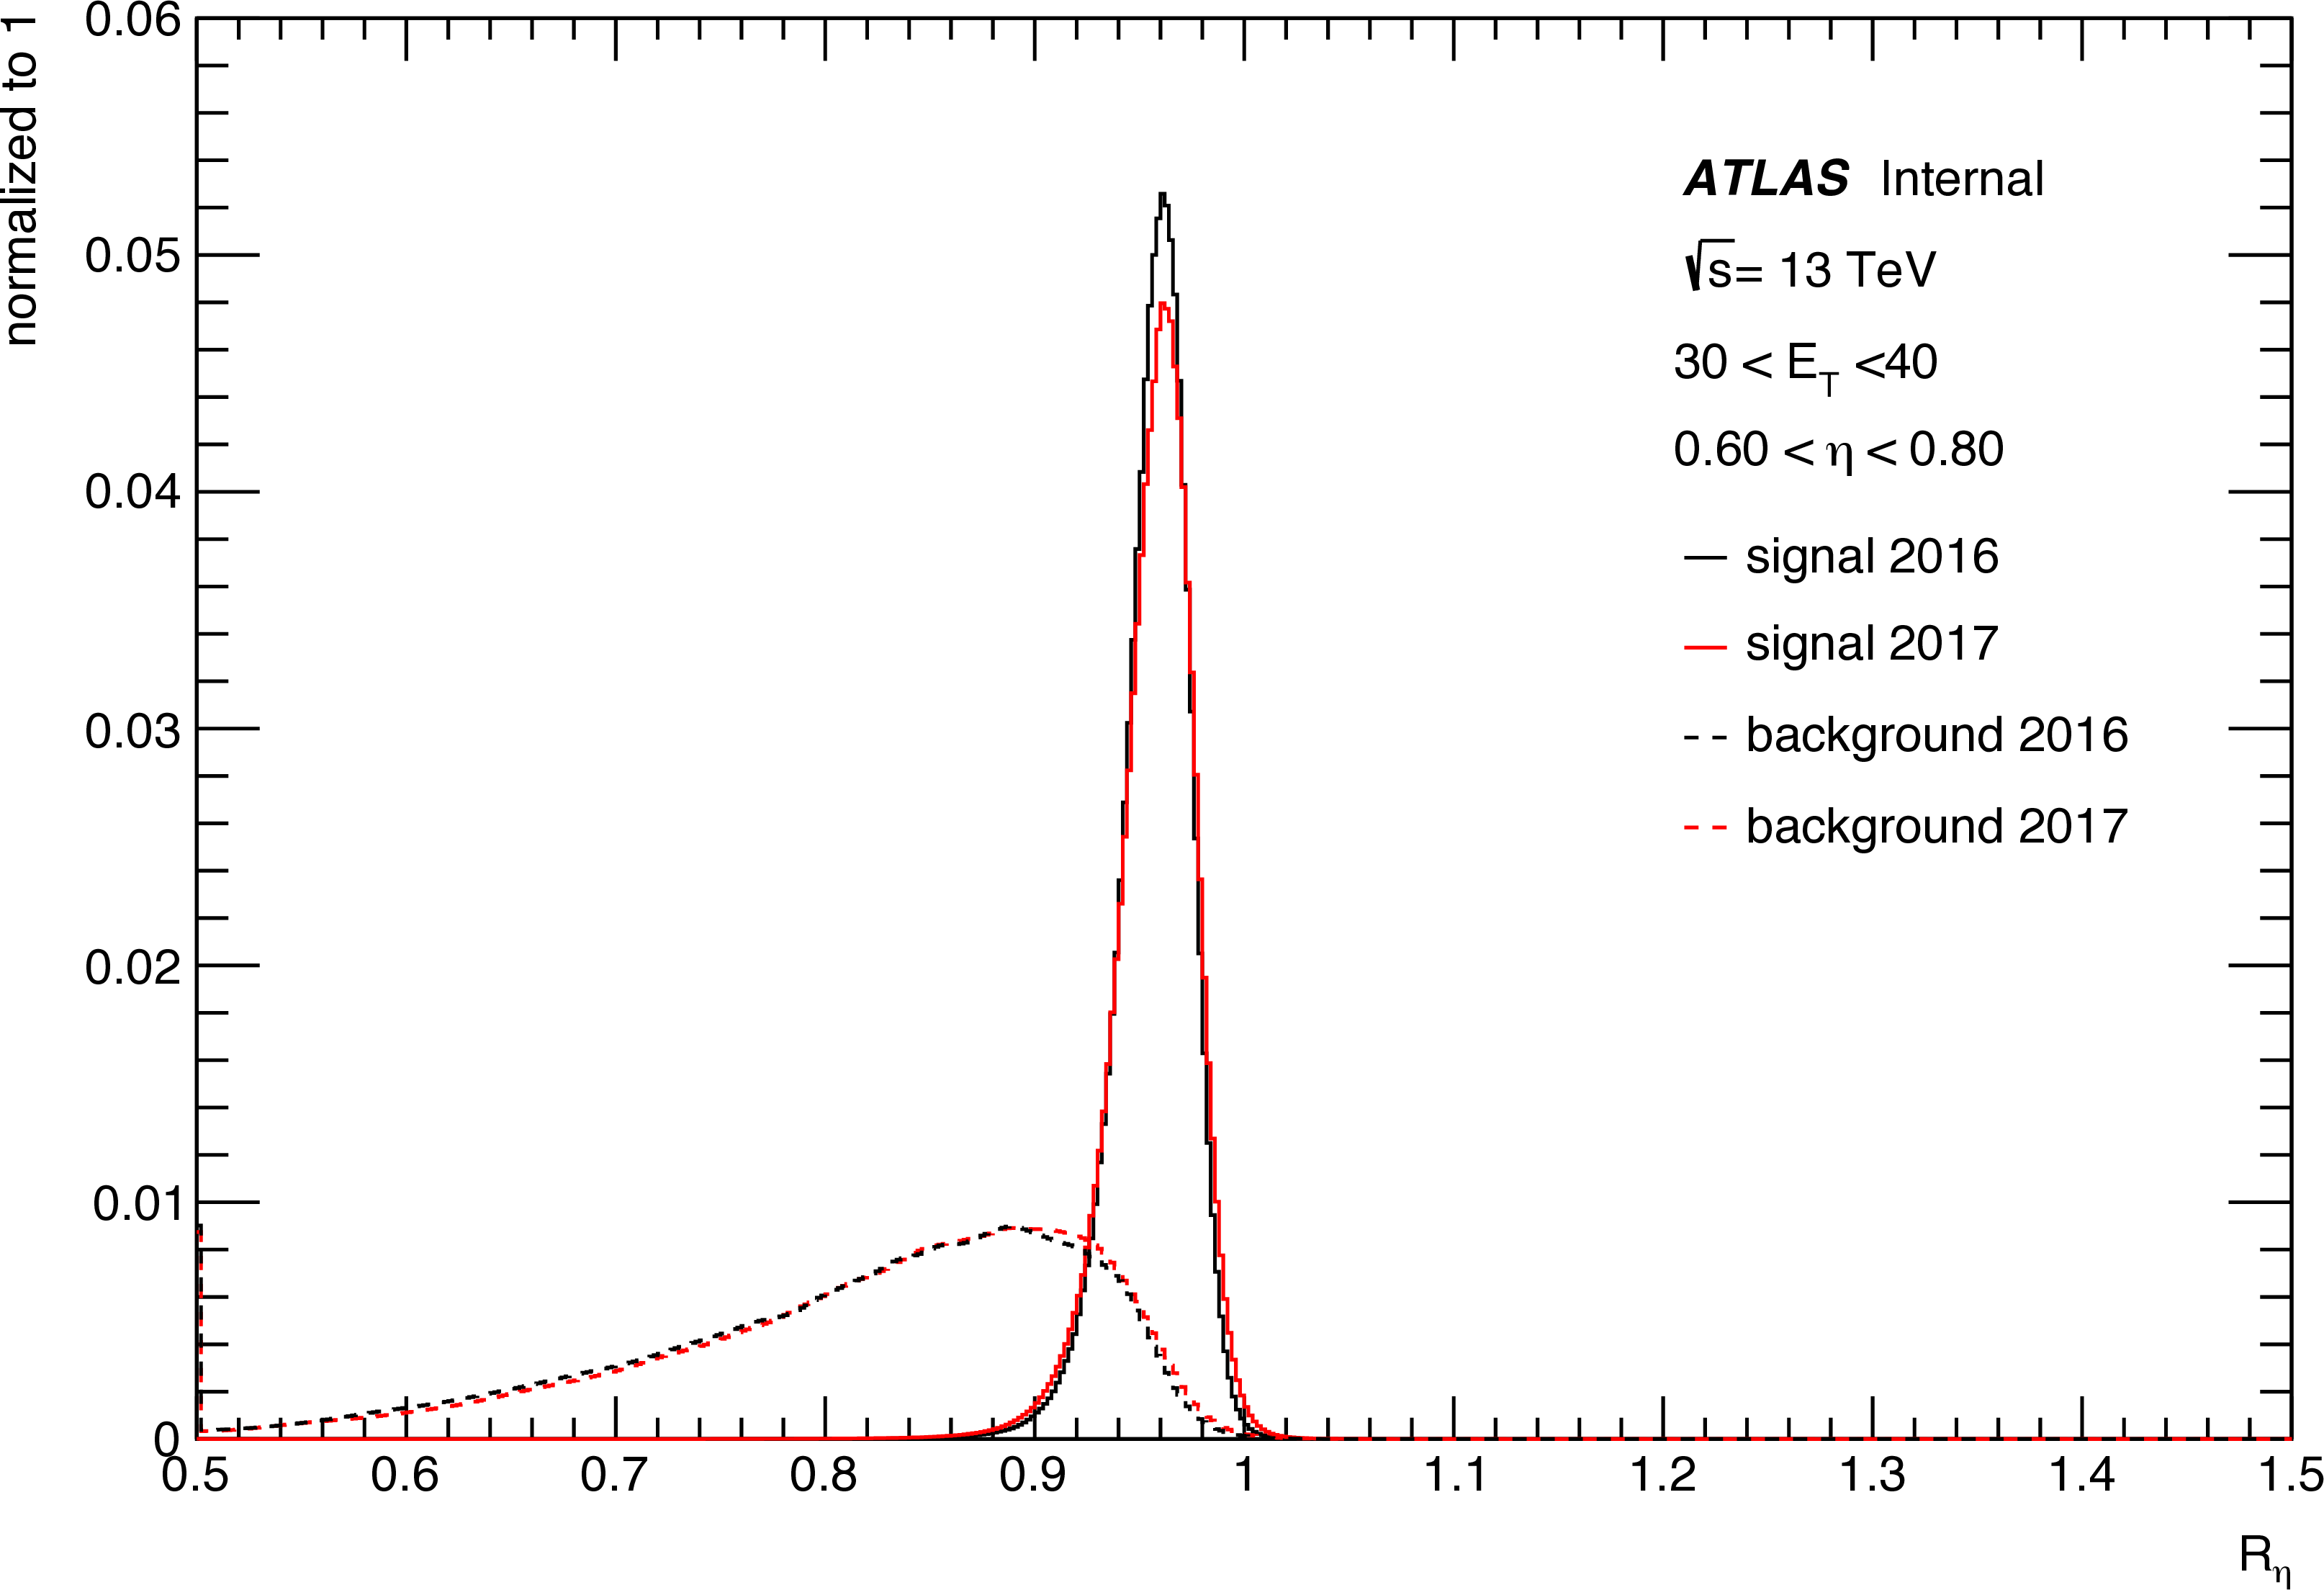
\includegraphics[width=1.0\textwidth]{figs/egamma/trig_reta_highet.png} 
    \label{fig:egamma:trig_reta}
  \end{subfigure}
  \caption[Pdfs of tracking and track-cluster matching variables \TRTPID, \deltaeta, \deltaphires, and the shower shape variables \weta, \rhad, and \reta.]{Pdfs of tracking and track-cluster matching variables \TRTPID, \deltaeta, \deltaphires, and the shower shape variables \weta, \rhad, and \reta.
  All of which are defined in Table~\ref{tab:IDcuts} and shown for
  30~\GeV $<$ \et\ $<$ 40~\GeV and $0.6<|\eta|<0.8$.
  The solid line distributions are determined from a background simulation sample and the dashed-line distributions are determined from a \Zee simulation sample.
  The black distributions are pdfs used in the trigger LH in 2016/2017 data taking years and the red are the pdfs developed for the 2018 year.
  These distributions are for reconstructed electron candidates before applying any identification.
  They are smoothed using an adaptive KDE and have been corrected for offsets or differences in widths between the distributions in data and simulation.
  }
\end{figure}
\begin{figure}[t]\ContinuedFloat
\centering
  \begin{subfigure}[b]{0.49\textwidth}
    \centering
    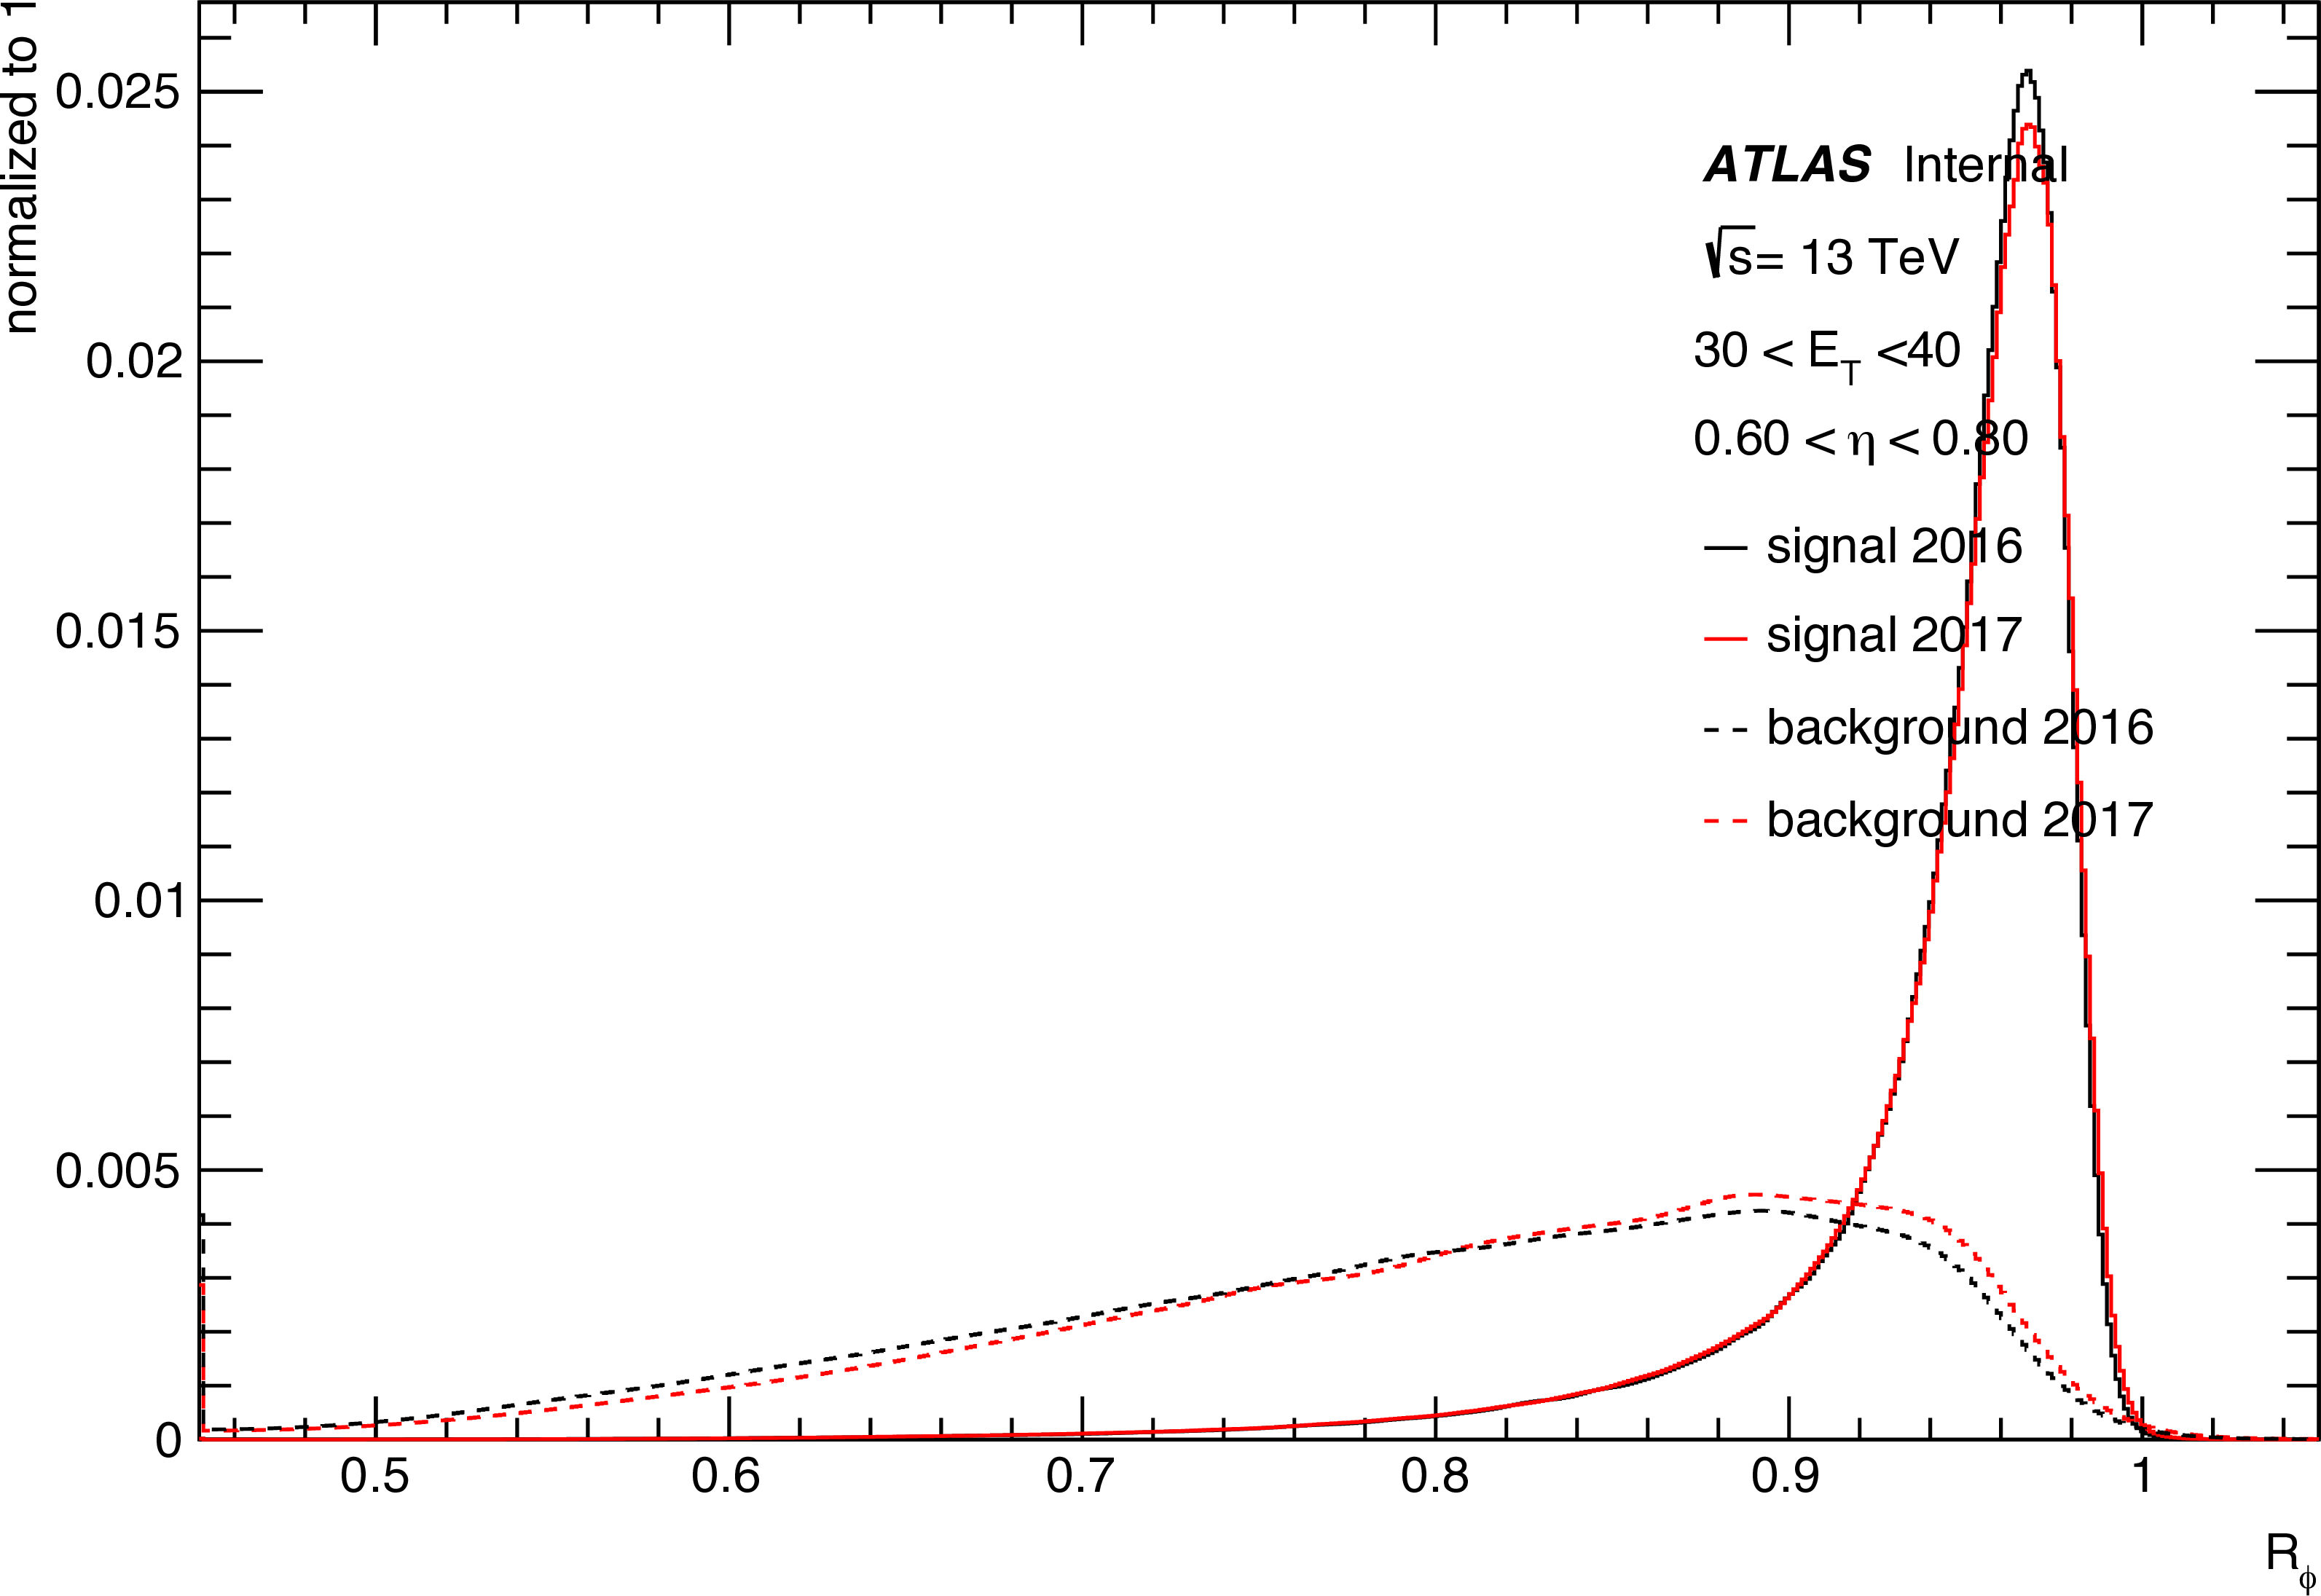
\includegraphics[width=1.0\textwidth]{figs/egamma/trig_rphi_highet.png} 
    \label{fig:egamma:trig_rphi}
  \end{subfigure}
  \hfill
  \begin{subfigure}[b]{0.49\textwidth}
    \centering
    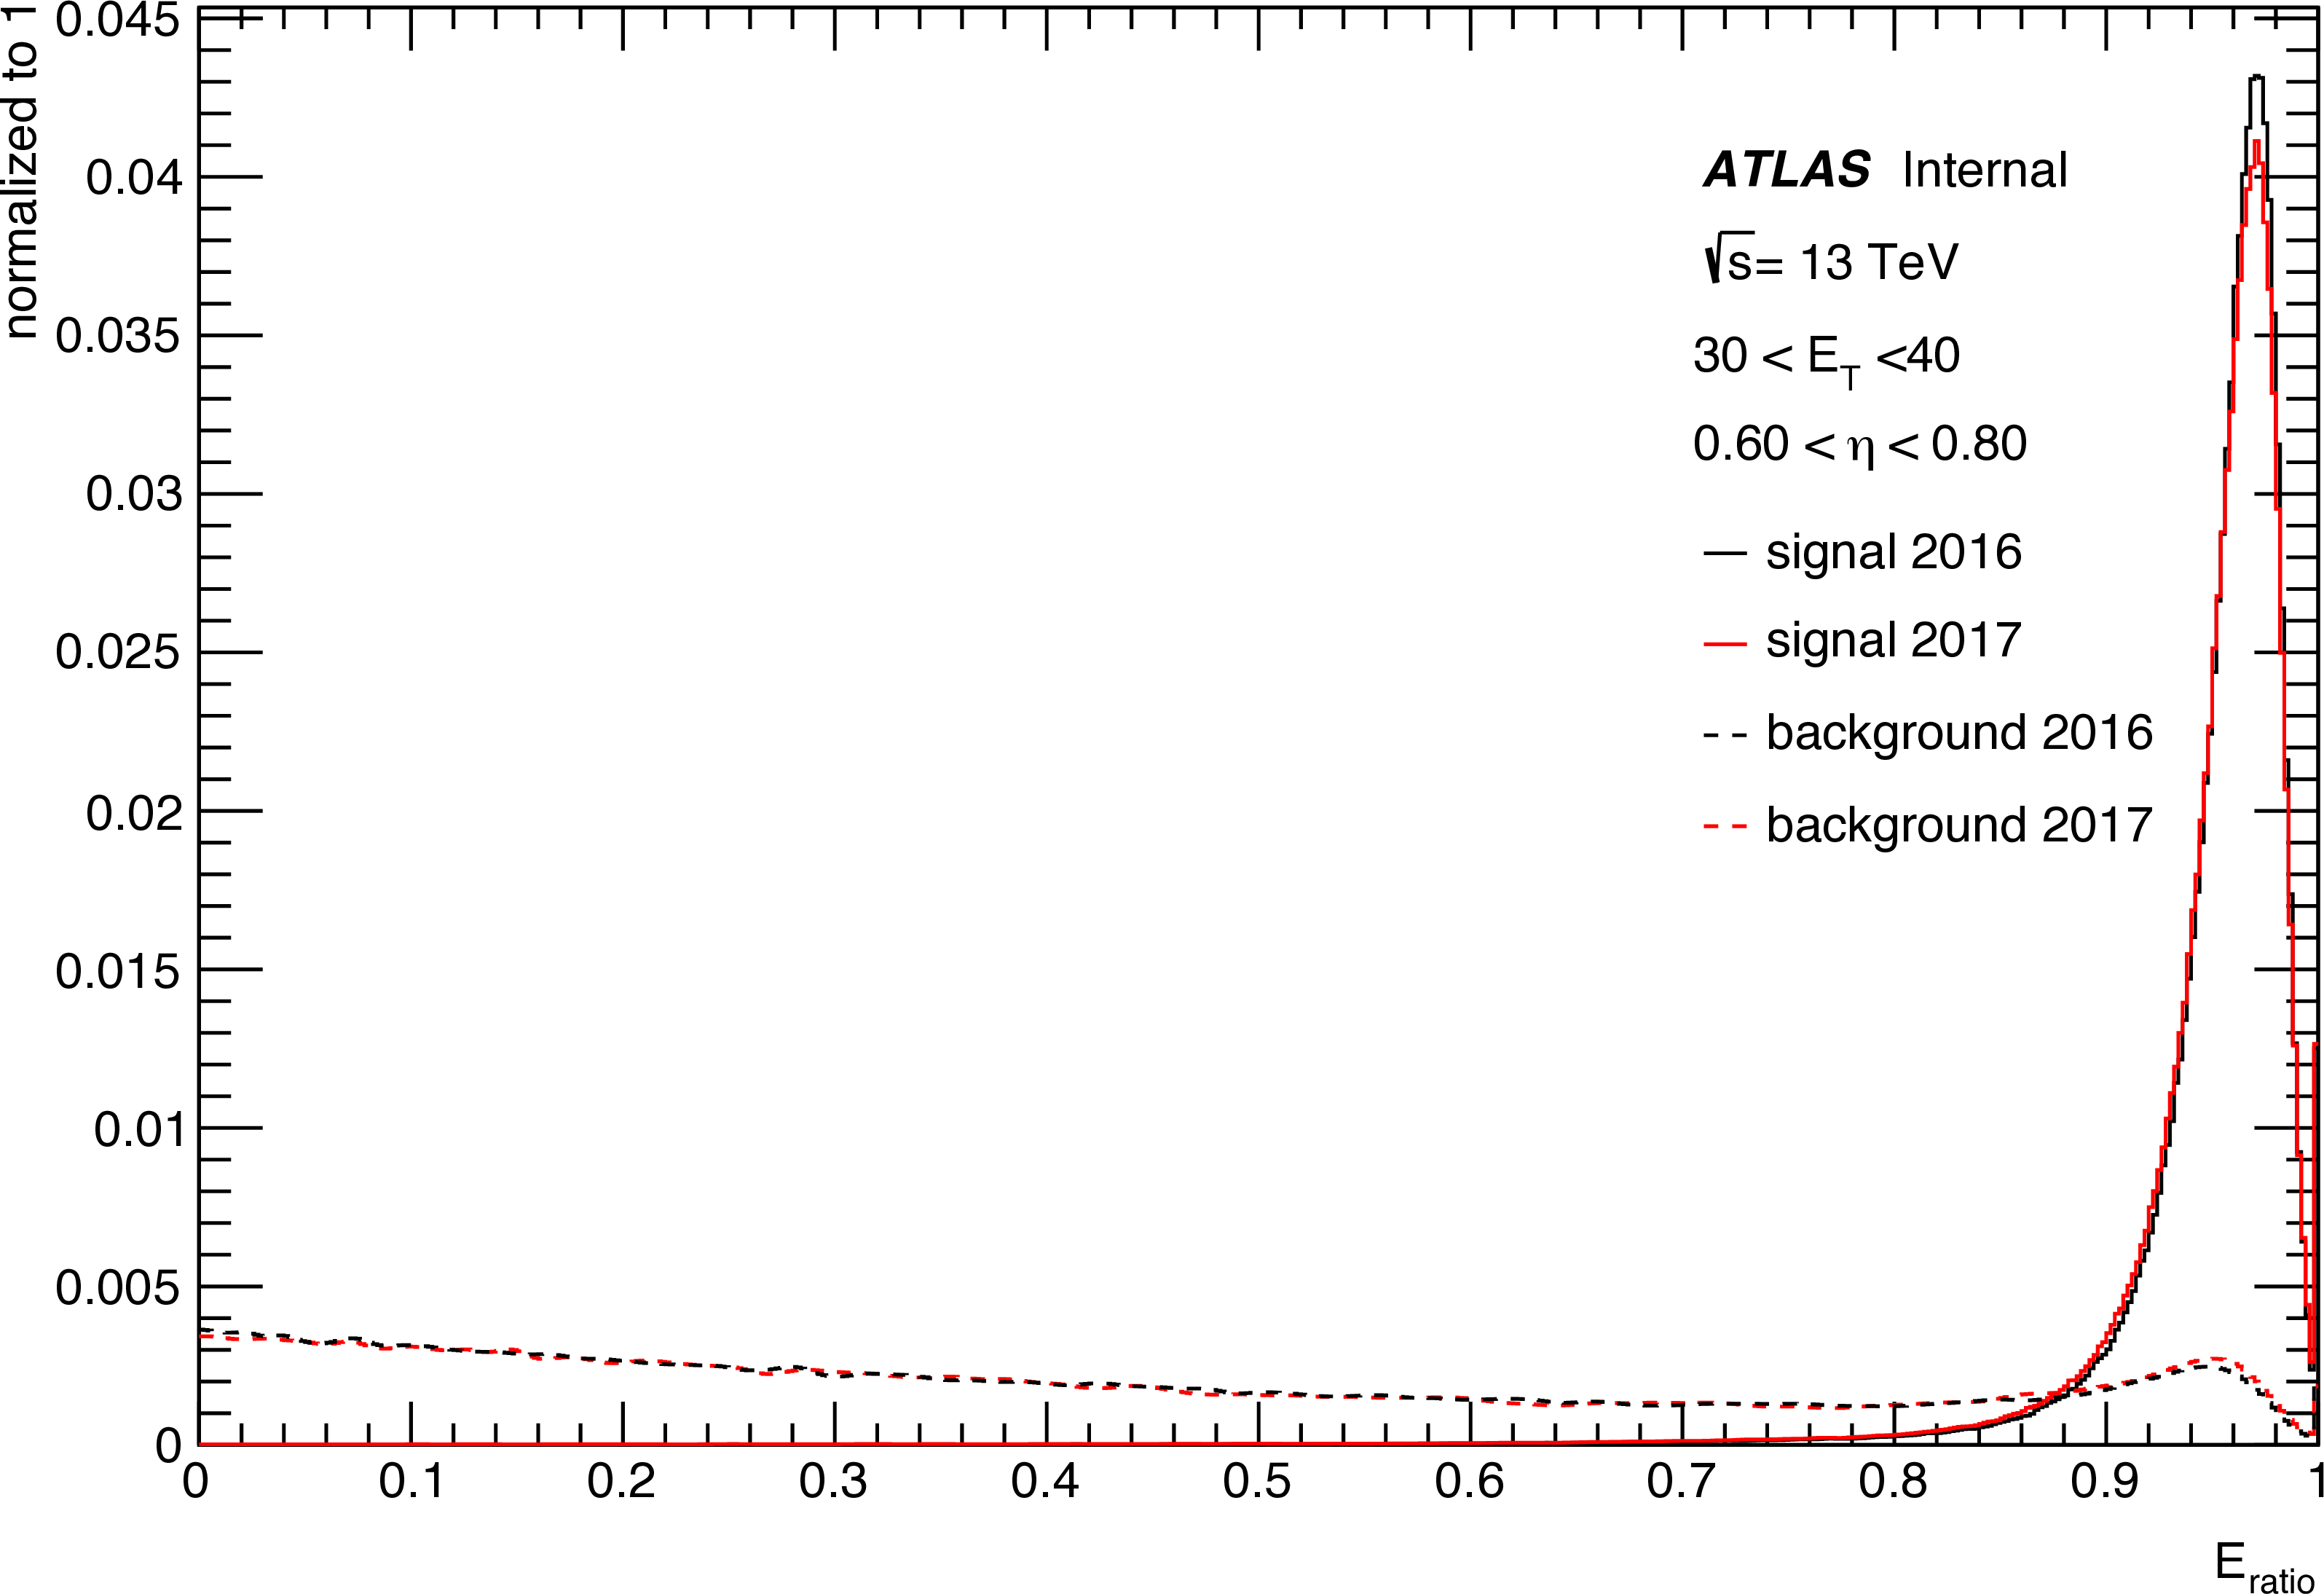
\includegraphics[width=1.0\textwidth]{figs/egamma/trig_eratio_highet.png} 
    \label{fig:egamma:trig_eratio}
  \end{subfigure}
  \hfill
  \begin{subfigure}[b]{0.49\textwidth}
    \centering
    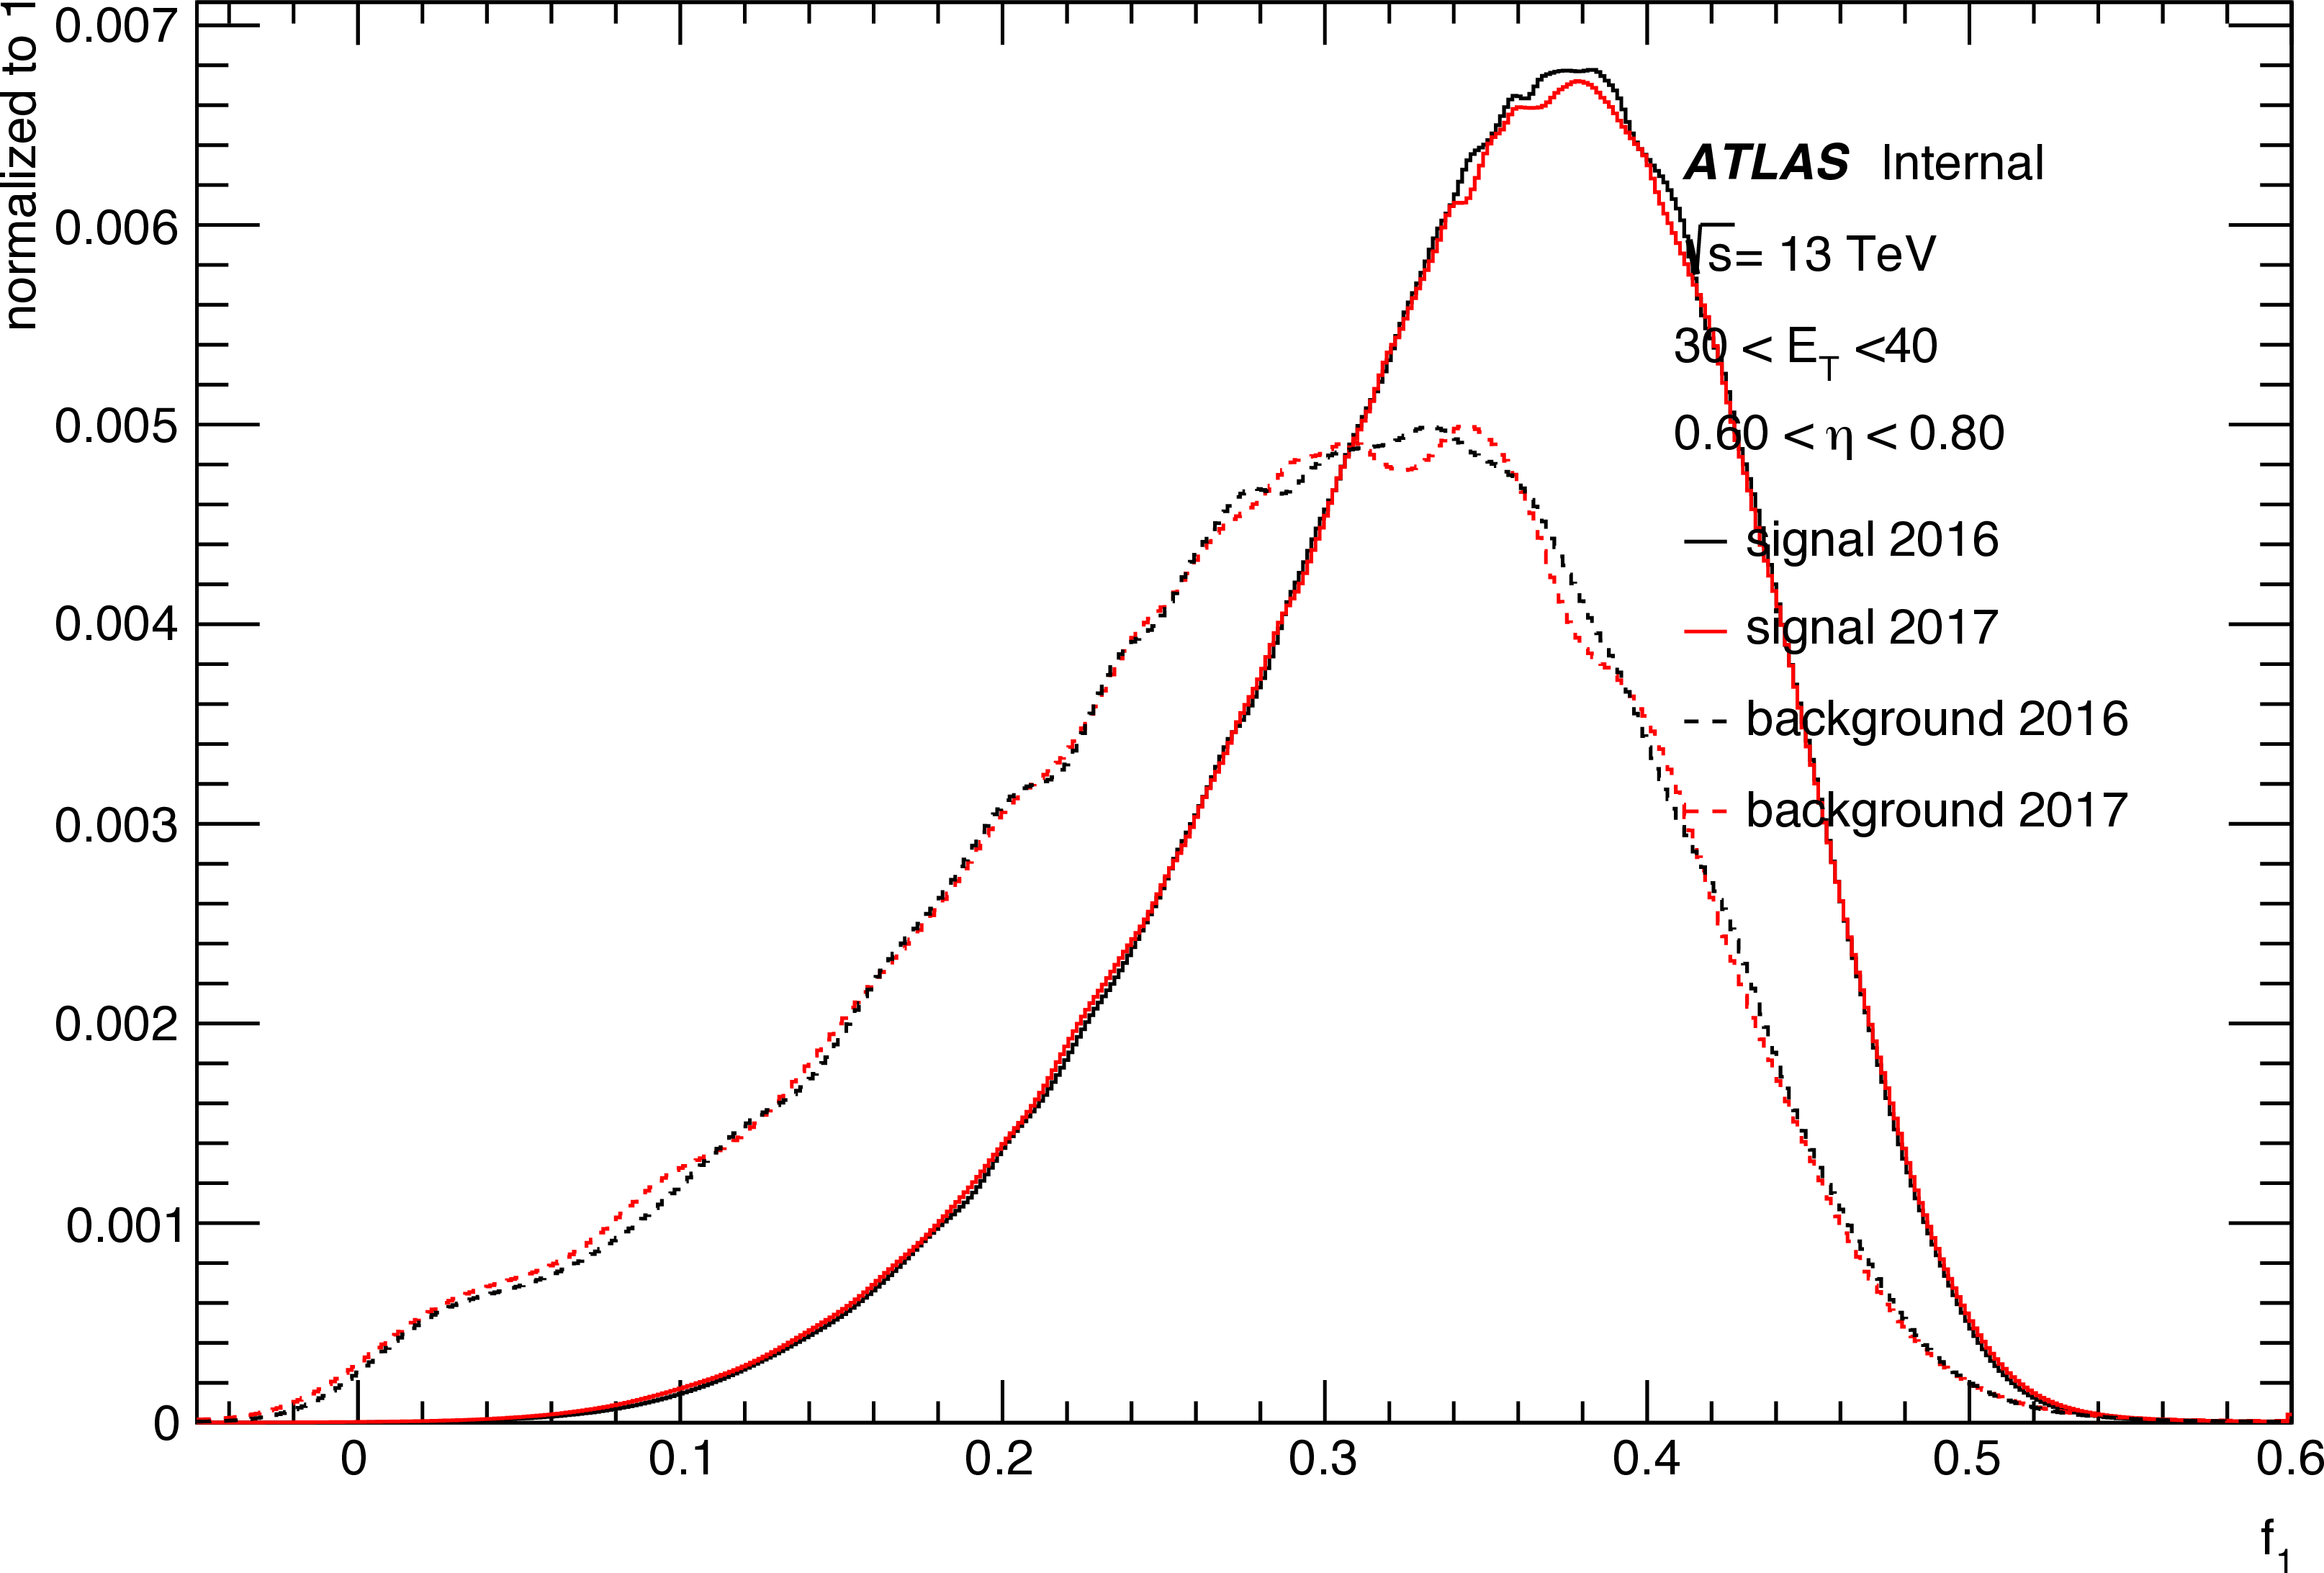
\includegraphics[width=1.0\textwidth]{figs/egamma/trig_f1_highet.png} 
    \label{fig:egamma:trig_f1}
  \end{subfigure}
  \hfill
  \begin{subfigure}[b]{0.49\textwidth}
    \centering
    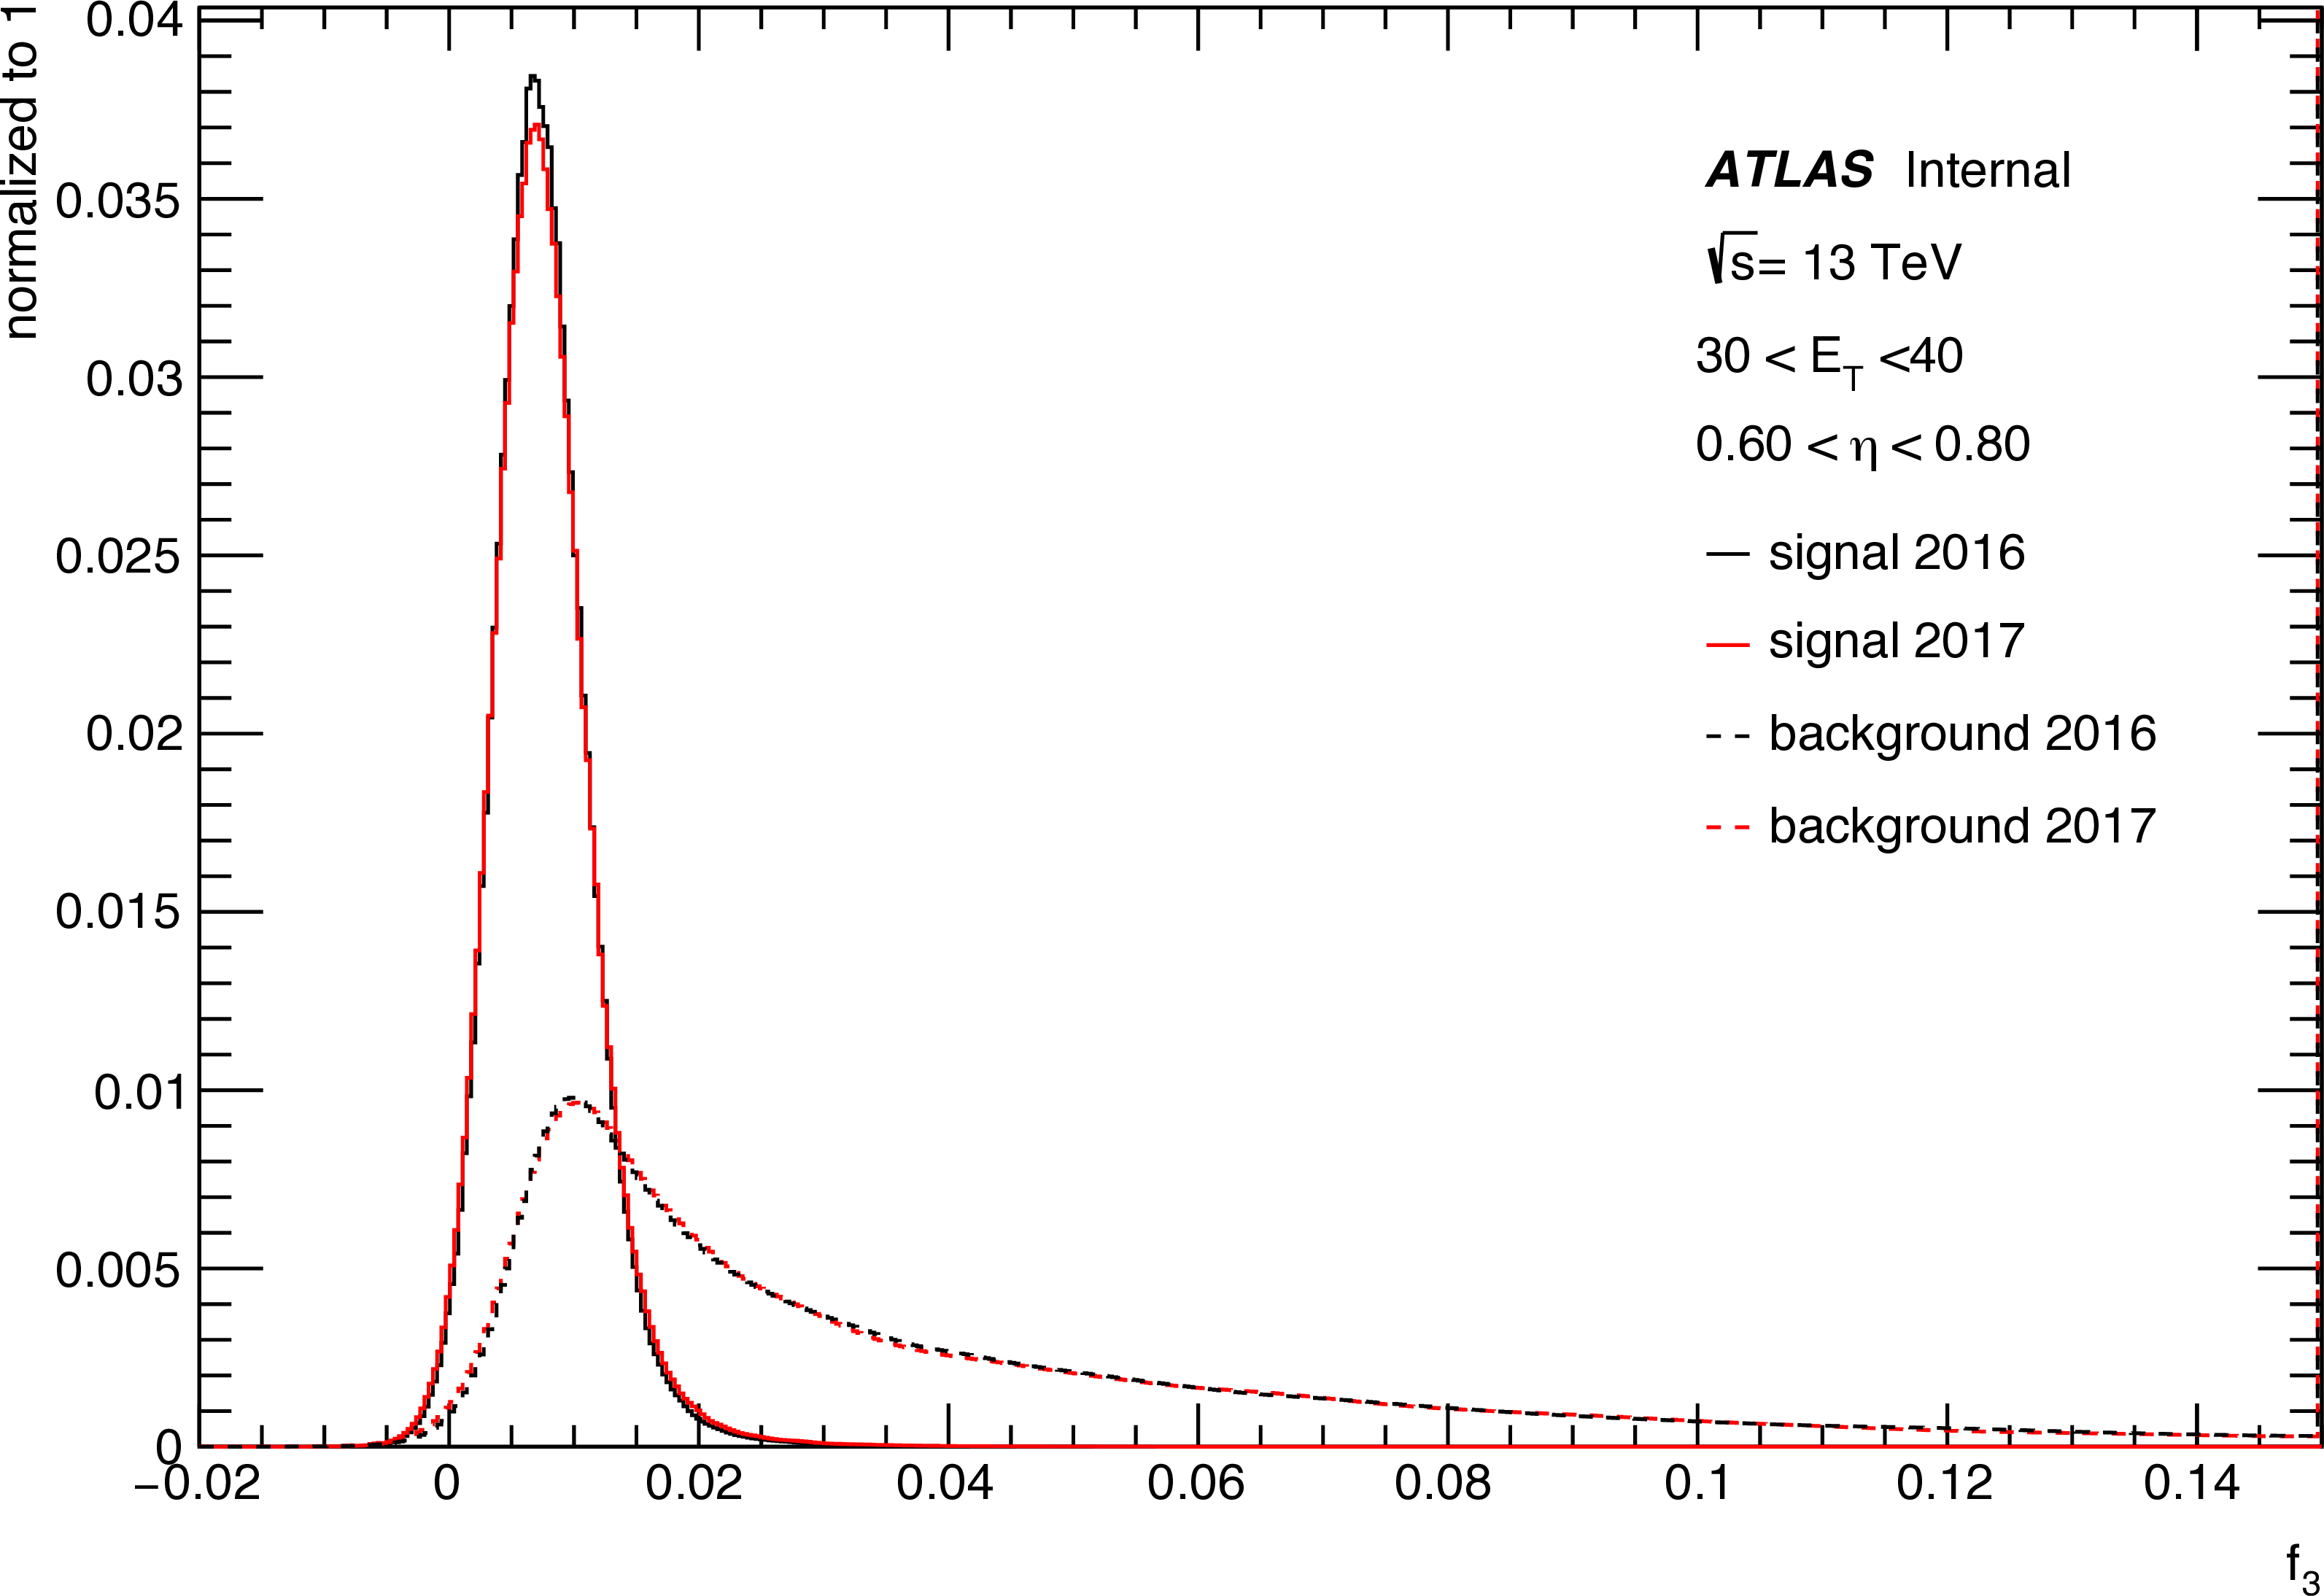
\includegraphics[width=1.0\textwidth]{figs/egamma/trig_f3_highet.png} 
    \label{fig:egamma:trig_f3}
  \end{subfigure}
  \caption[Pdfs of shower shape variables \rphi, $E_{\mathrm{ratio}}$, \fI, and \fIII]{Pdfs of shower shape variables \rphi, $E_{\mathrm{ratio}}$, \fI, and \fIII.
  All of which are defined in Table~\ref{tab:IDcuts} and shown for
  30~\GeV $<$ \et\ $<$ 40~\GeV and $0.6<|\eta|<0.8$.
  The solid line distributions are determined from a background simulation sample and the dashed-line distributions are determined from a \Zee simulation sample.
  The black distributions are pdfs used in the trigger LH in 2016/2017 data taking years and the red are the pdfs developed for the 2018 year.
  These distributions are for reconstructed electron candidates before applying any identification.
  They are smoothed using an adaptive KDE and have been corrected for offsets or differences in widths between the distributions in data and simulation.
}
\label{fig:egamma:trig_pdfs_highet}
\end{figure}
\begin{figure}[p]
\centering
  \begin{subfigure}[b]{0.49\textwidth}
    \centering
    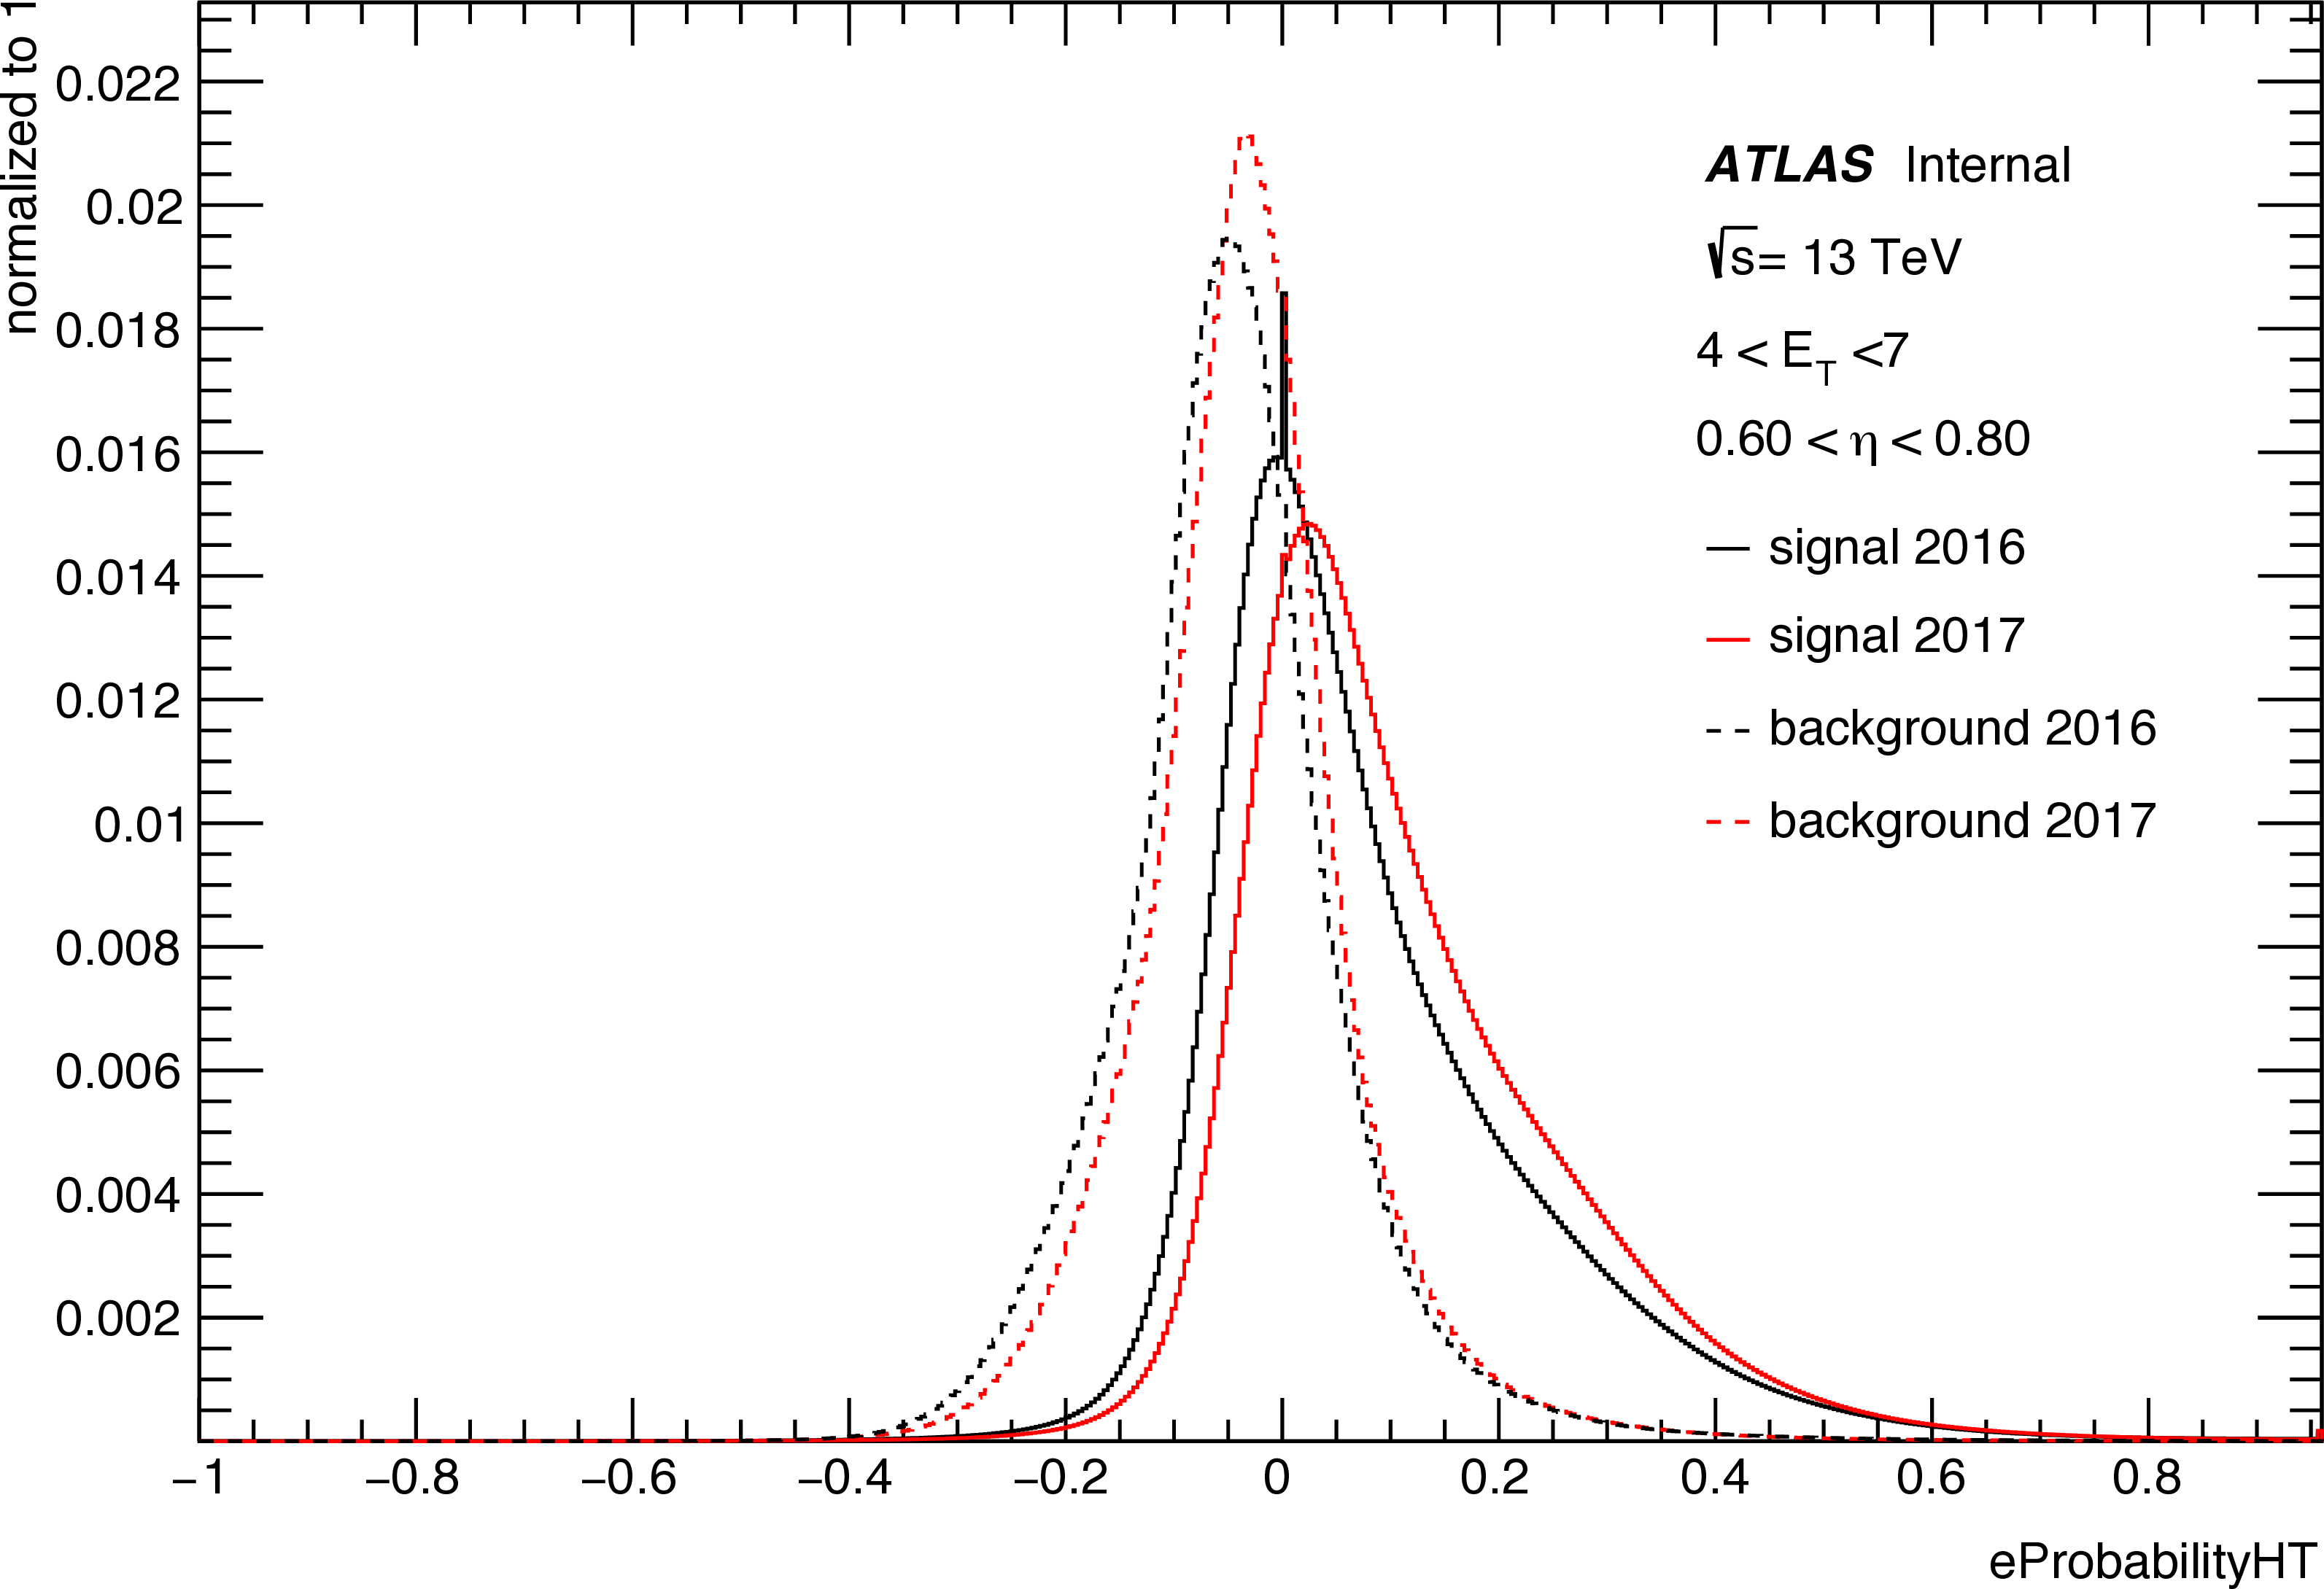
\includegraphics[width=1.0\textwidth]{figs/egamma/trig_eProb_lowet.png} 
    \label{fig:egamma:trig_eProbHT_lowet}
  \end{subfigure}
  \hfill
  \begin{subfigure}[b]{0.49\textwidth}
    \centering
    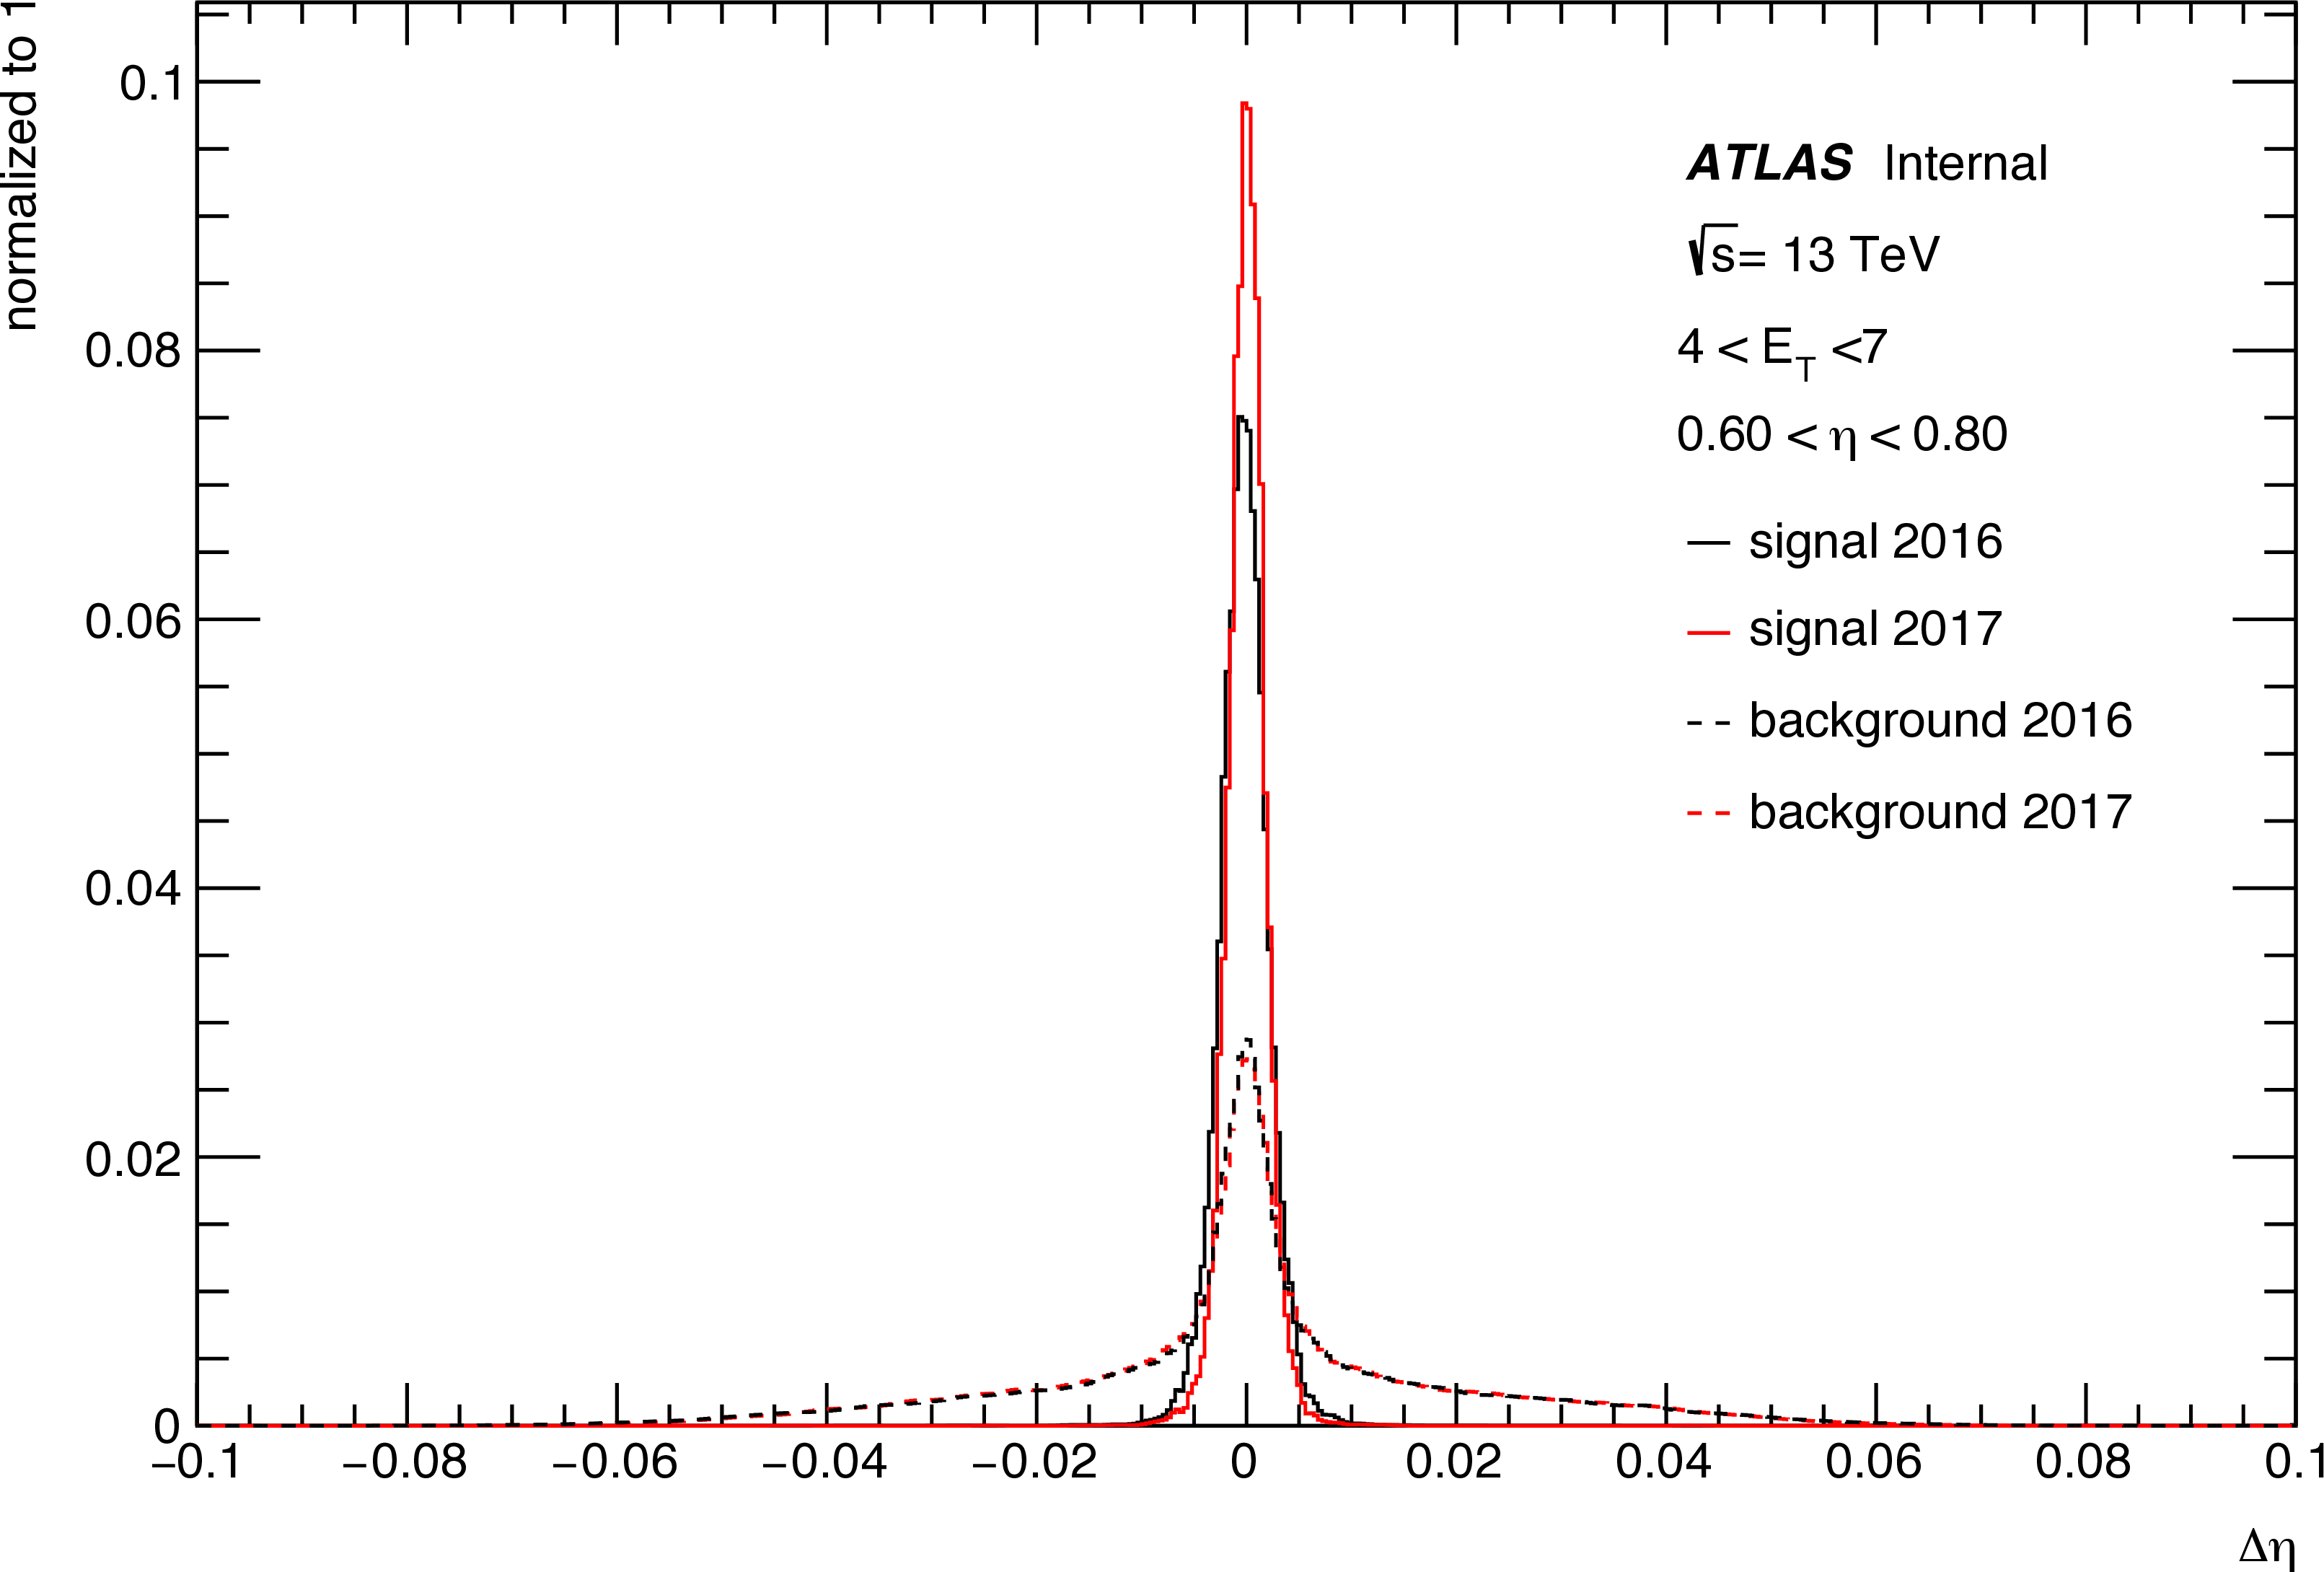
\includegraphics[width=1.0\textwidth]{figs/egamma/trig_deltaeta_lowet.png} 
    \label{fig:egamma:trig_deltaEta_1_lowet}
  \end{subfigure}
  \hfill
  \begin{subfigure}[b]{0.49\textwidth}
    \centering
    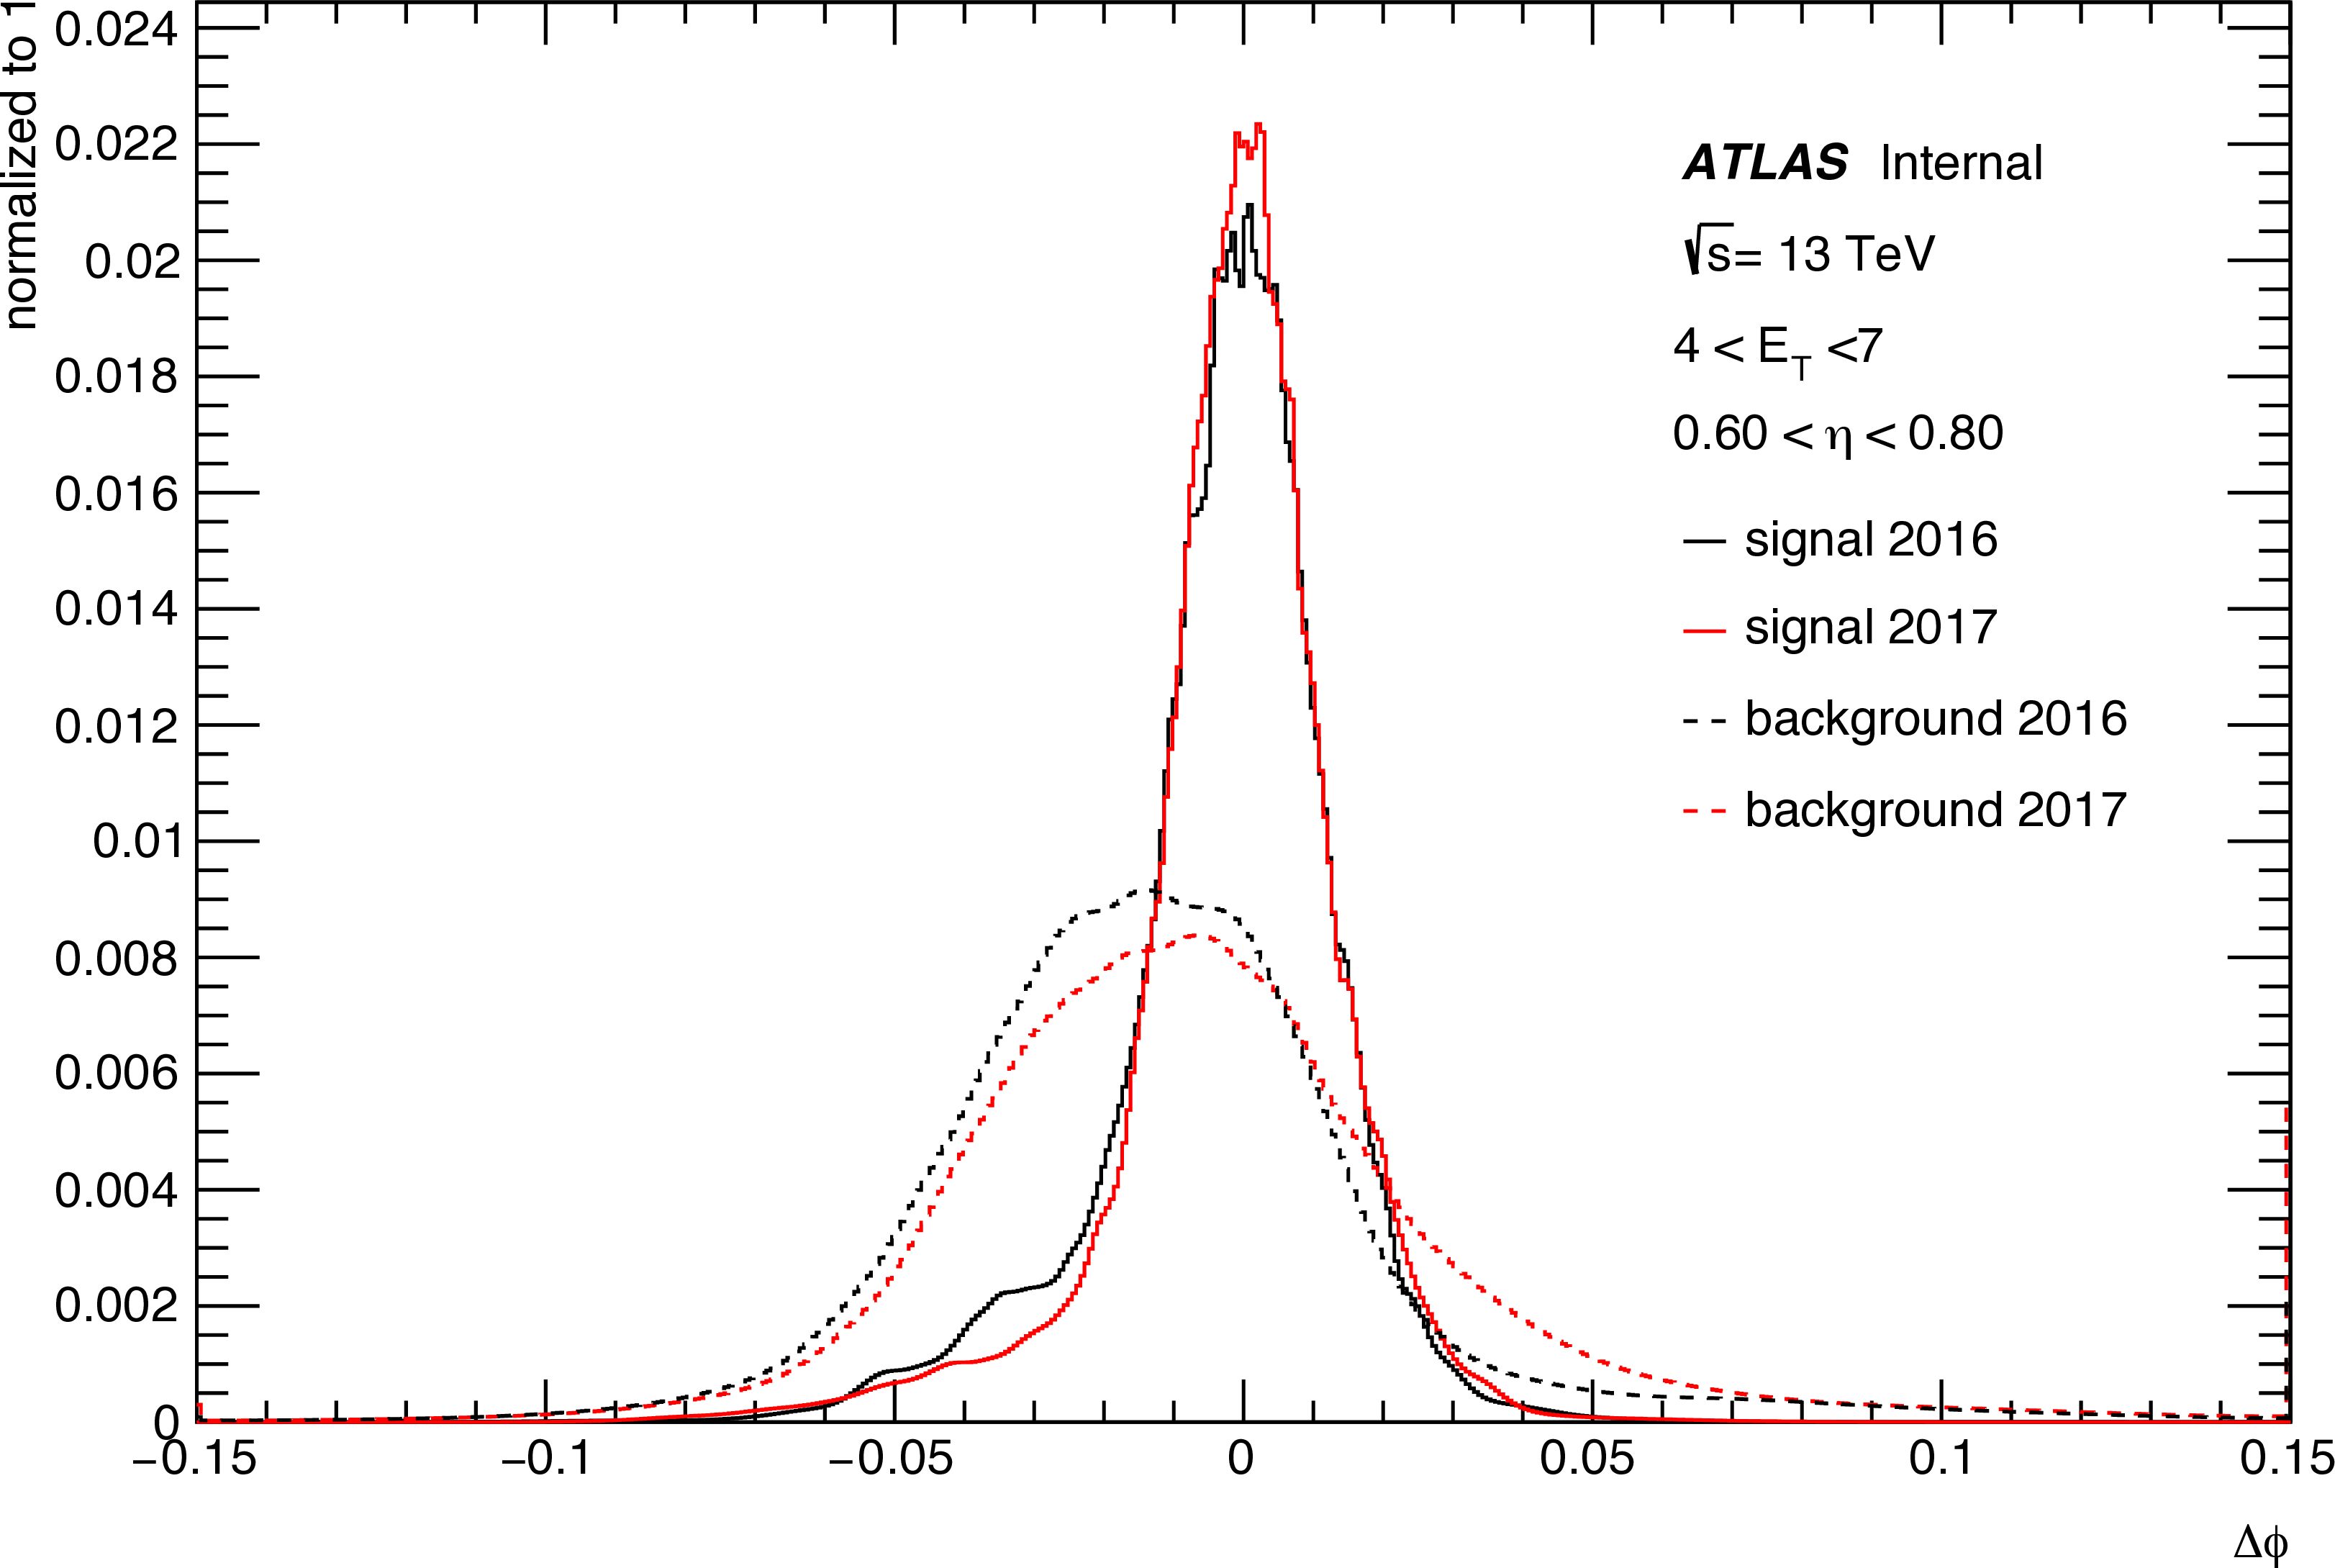
\includegraphics[width=1.0\textwidth]{figs/egamma/trig_deltaphi_lowet.png} 
    \label{fig:egamma:trig_deltaPhi_res_lowet}
  \end{subfigure}
  \hfill
  \begin{subfigure}[b]{0.49\textwidth}
    \centering
    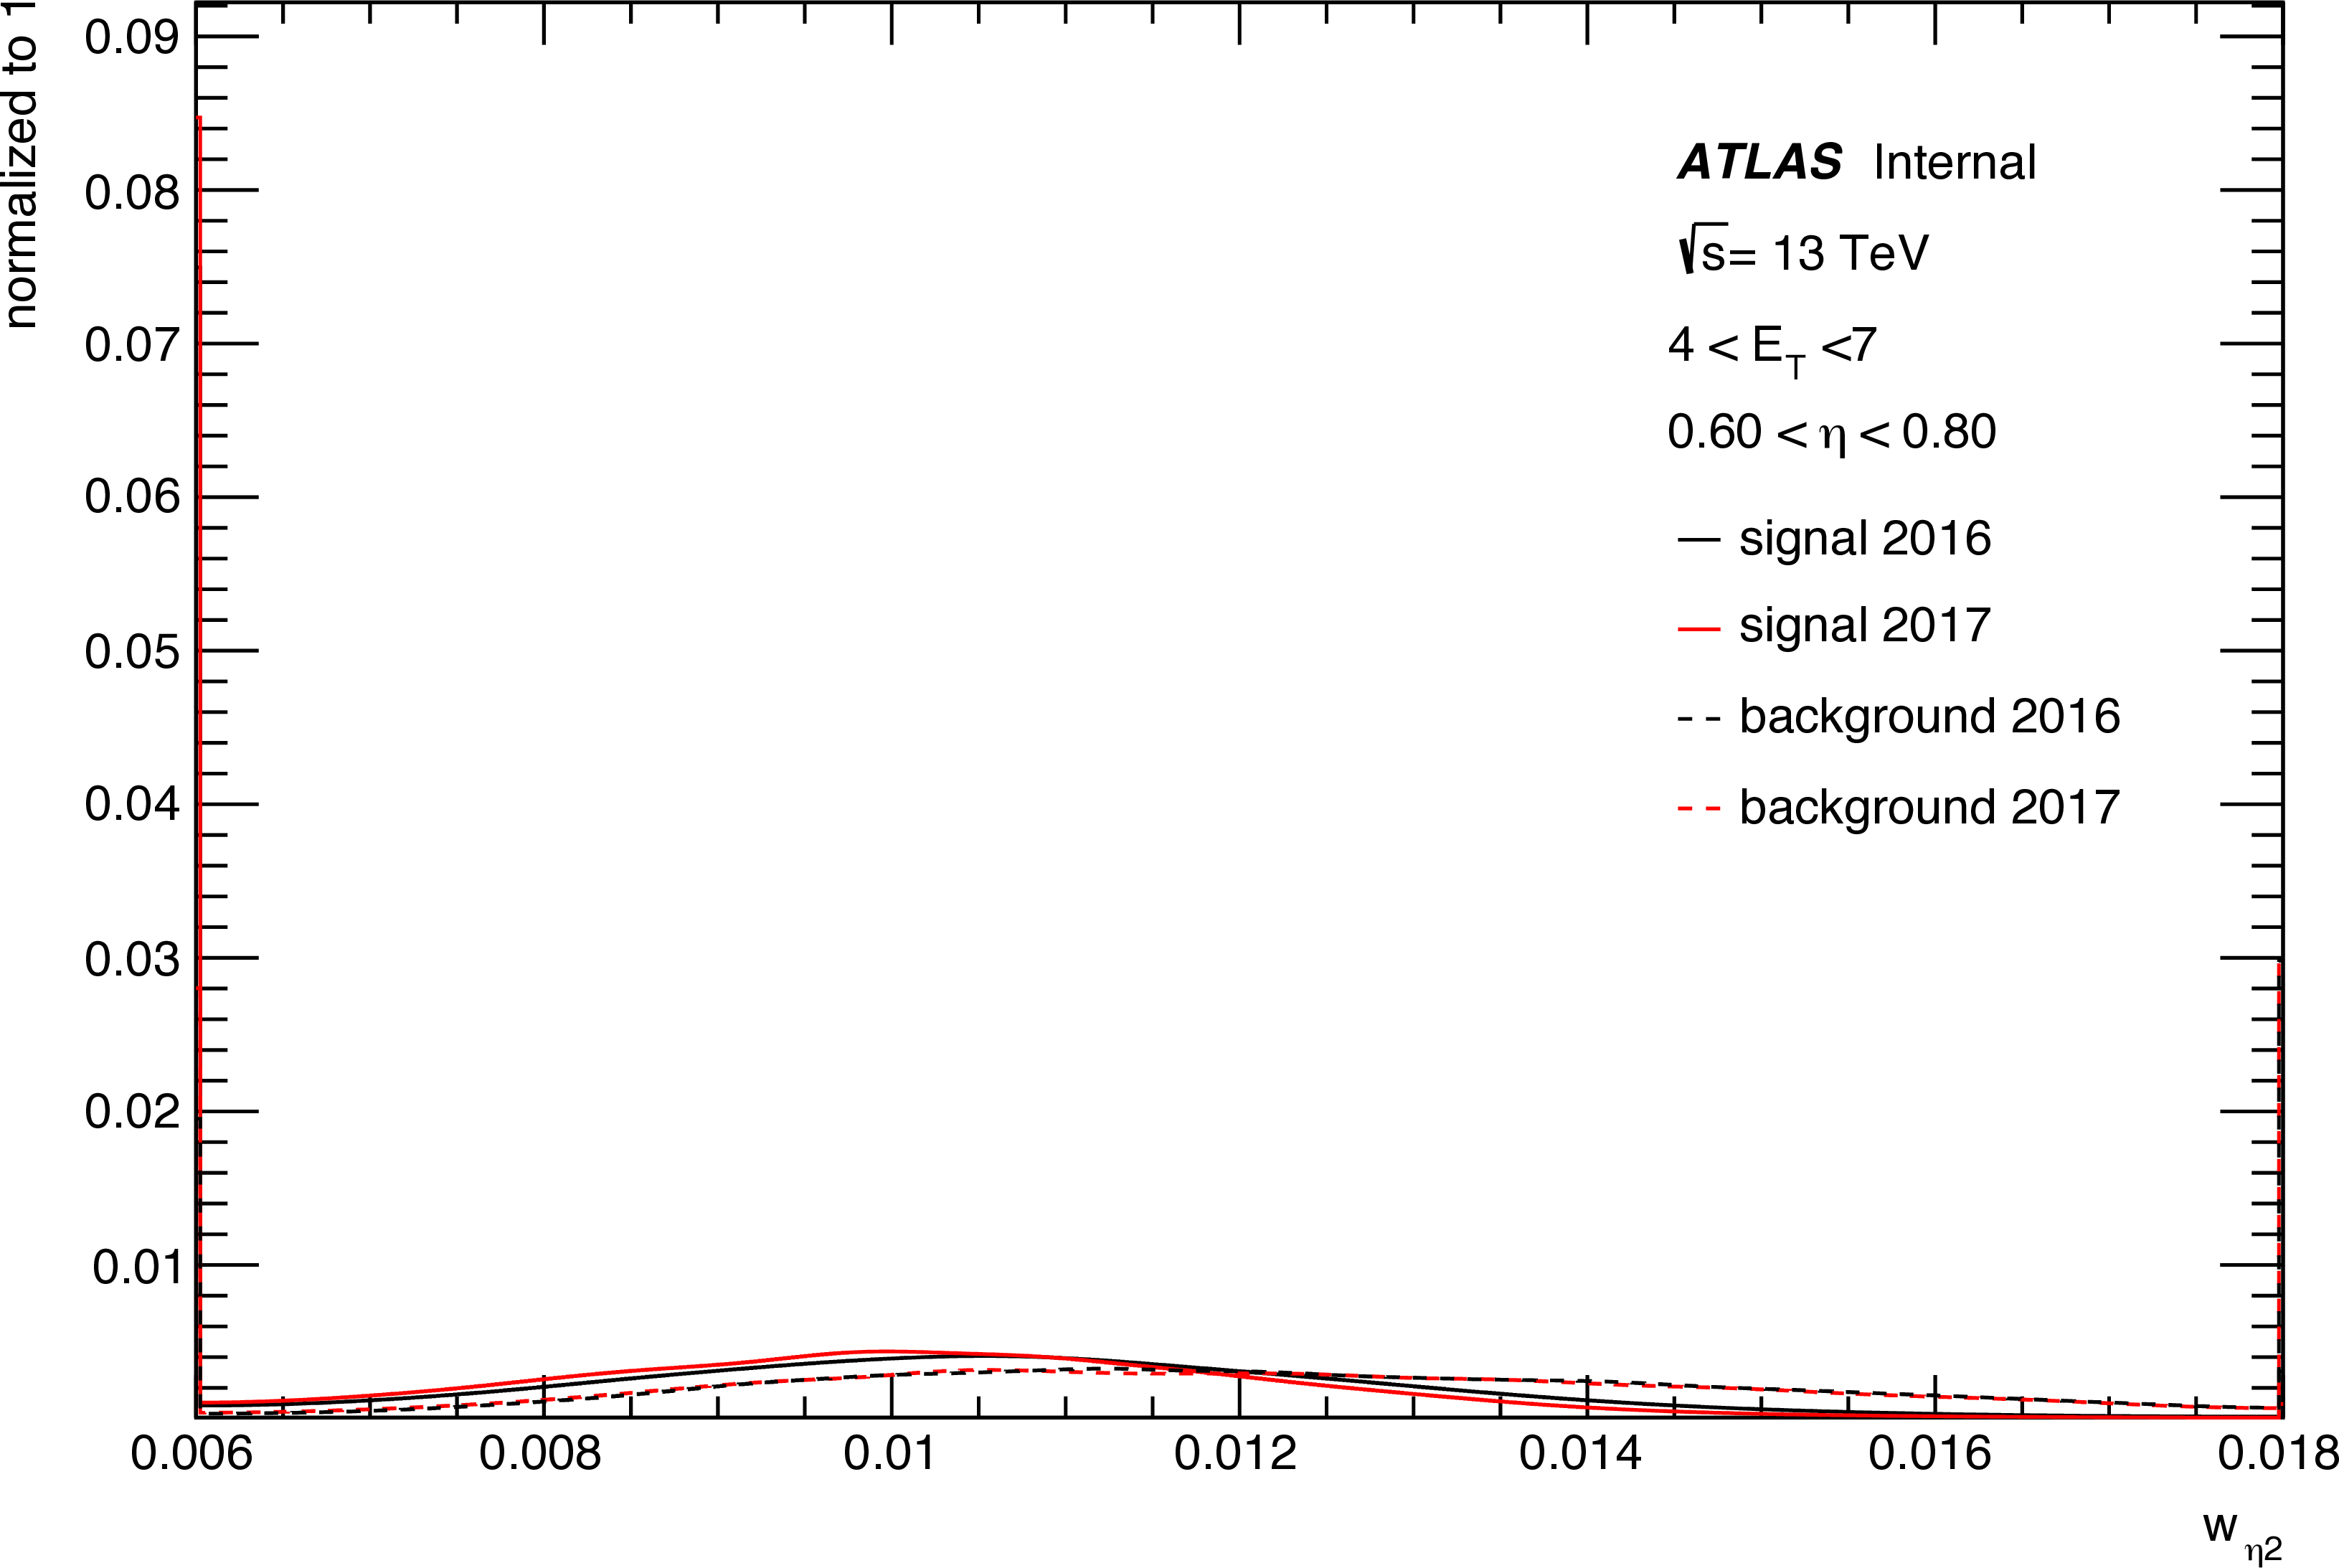
\includegraphics[width=1.0\textwidth]{figs/egamma/trig_weta2_lowet.png} 
    \label{fig:egamma:trig_weta2_lowet}
  \end{subfigure}
  \begin{subfigure}[b]{0.49\textwidth}
      \centering
    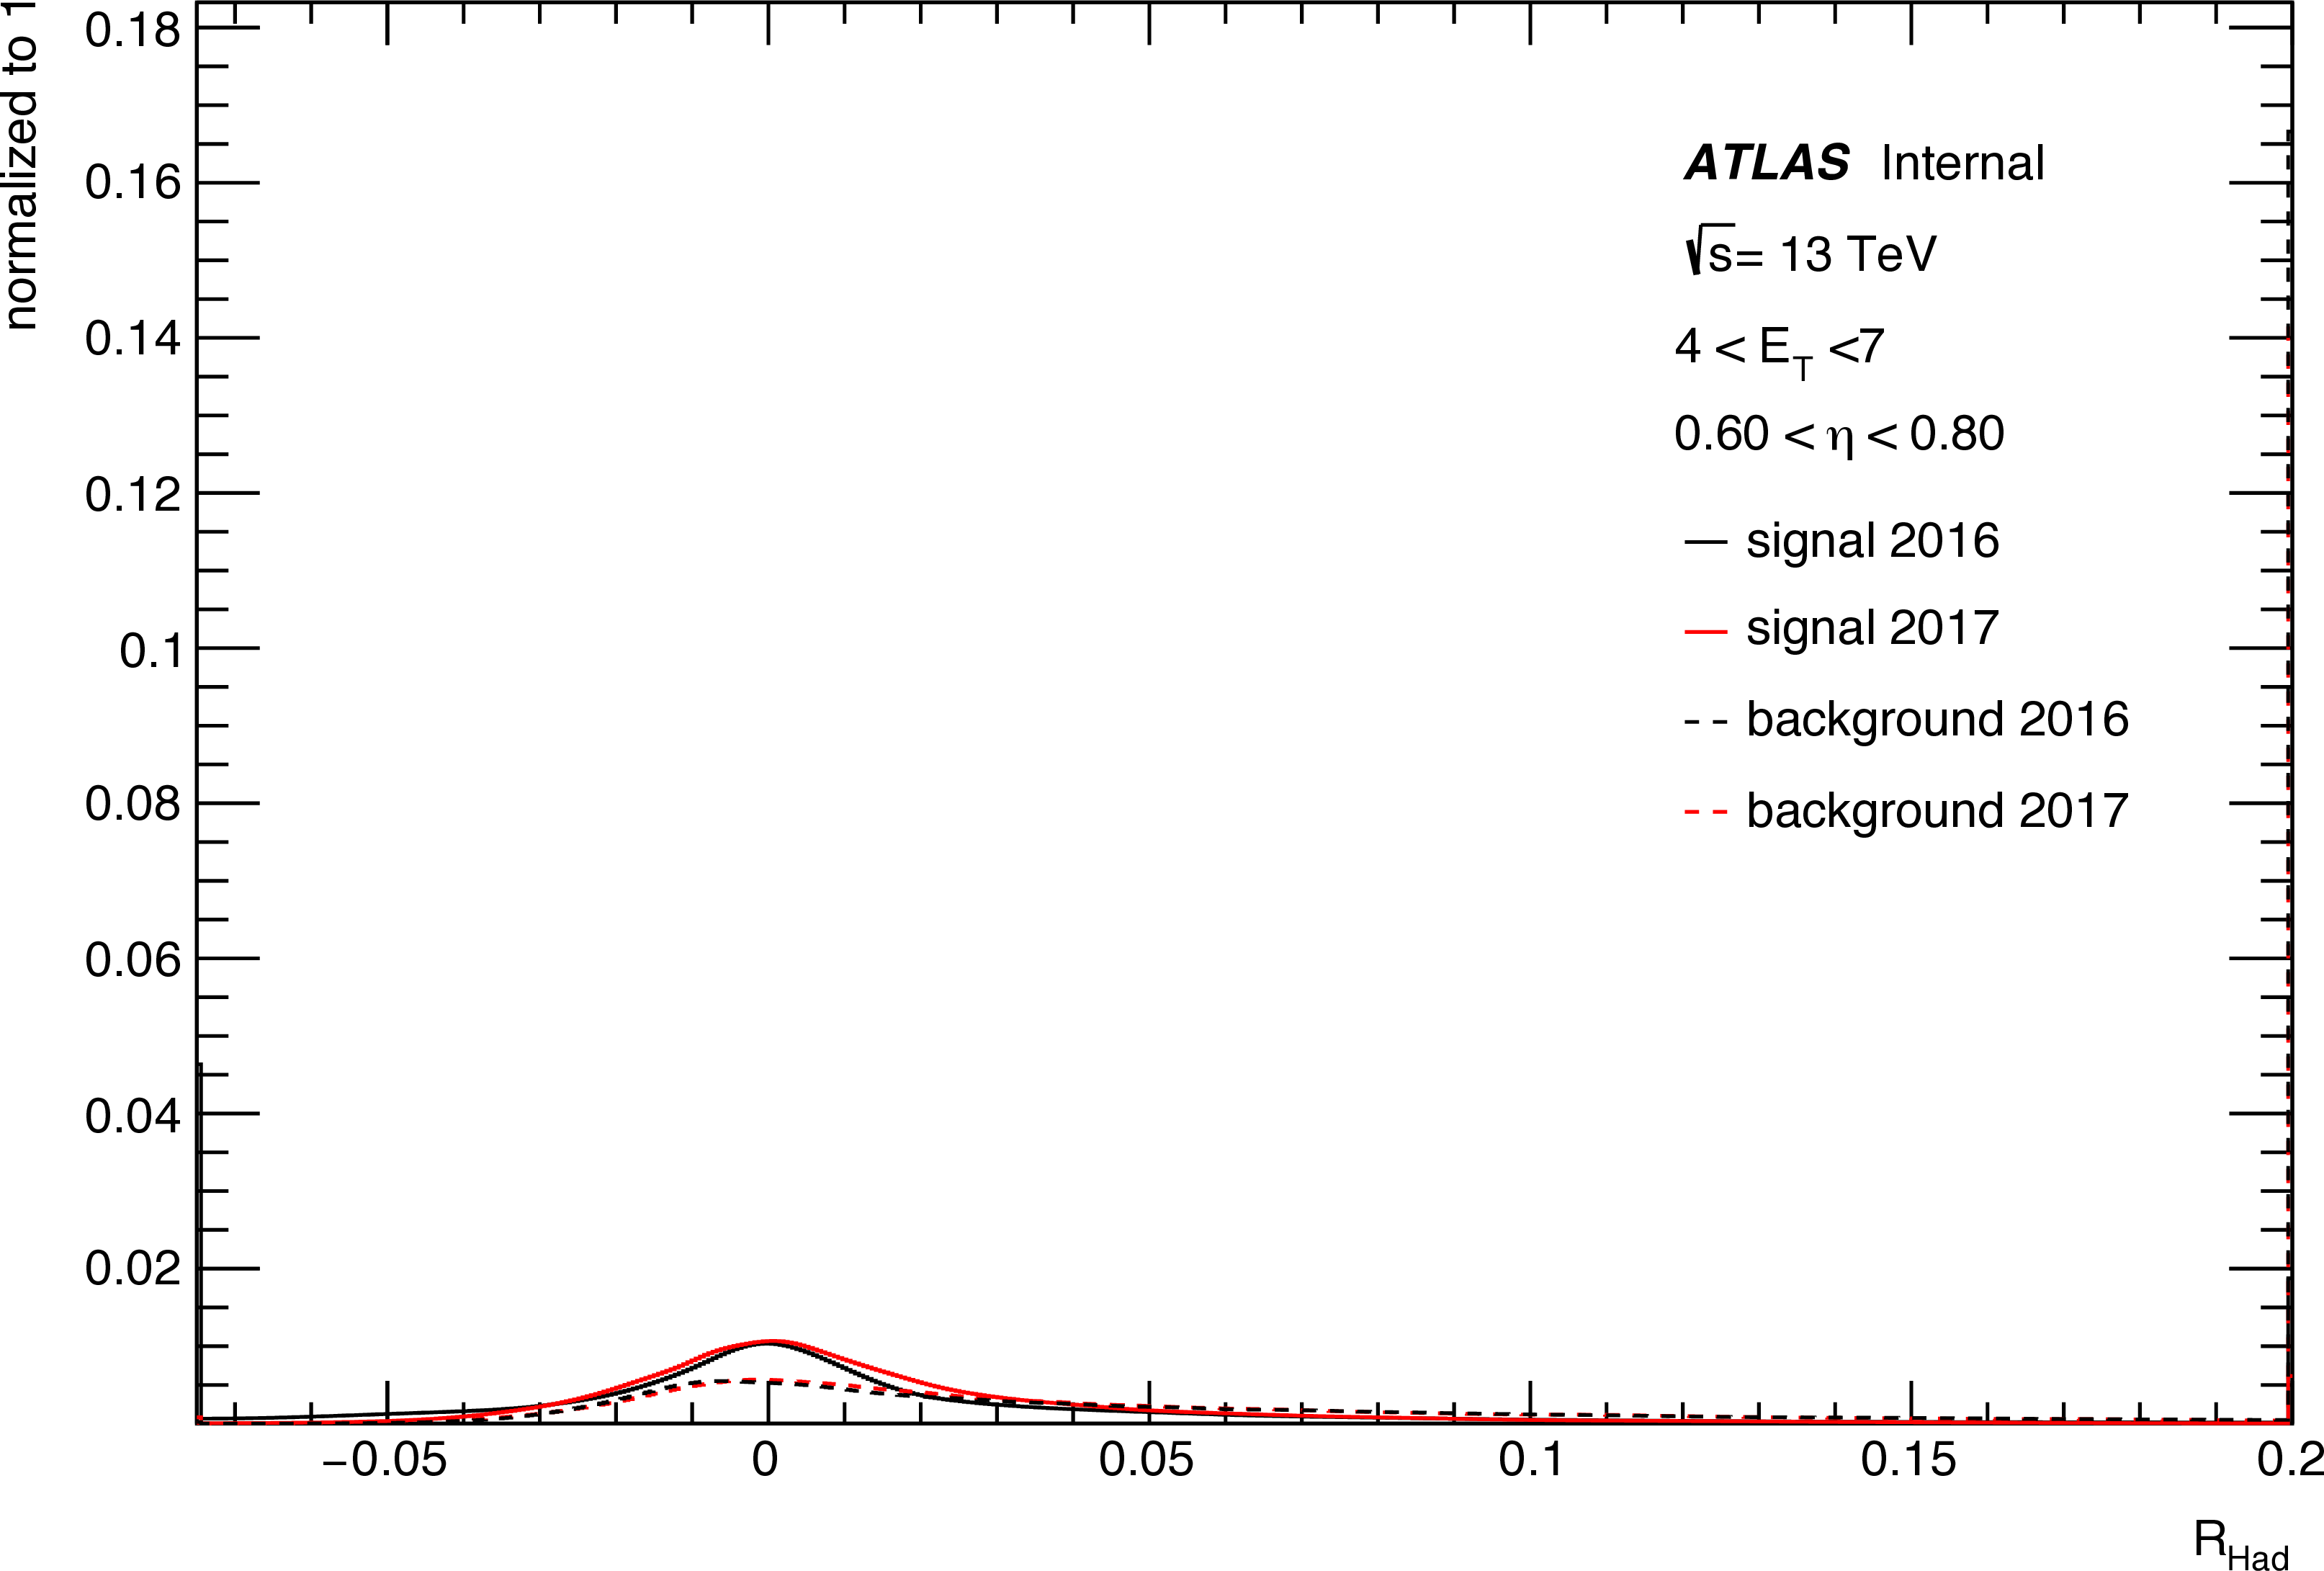
\includegraphics[width=1.0\textwidth]{figs/egamma/trig_rhad_lowet.png} 
    \label{fig:egamma:trig_rhad_lowet}
  \end{subfigure}
  \hfill
  \begin{subfigure}[b]{0.49\textwidth}
    \centering
    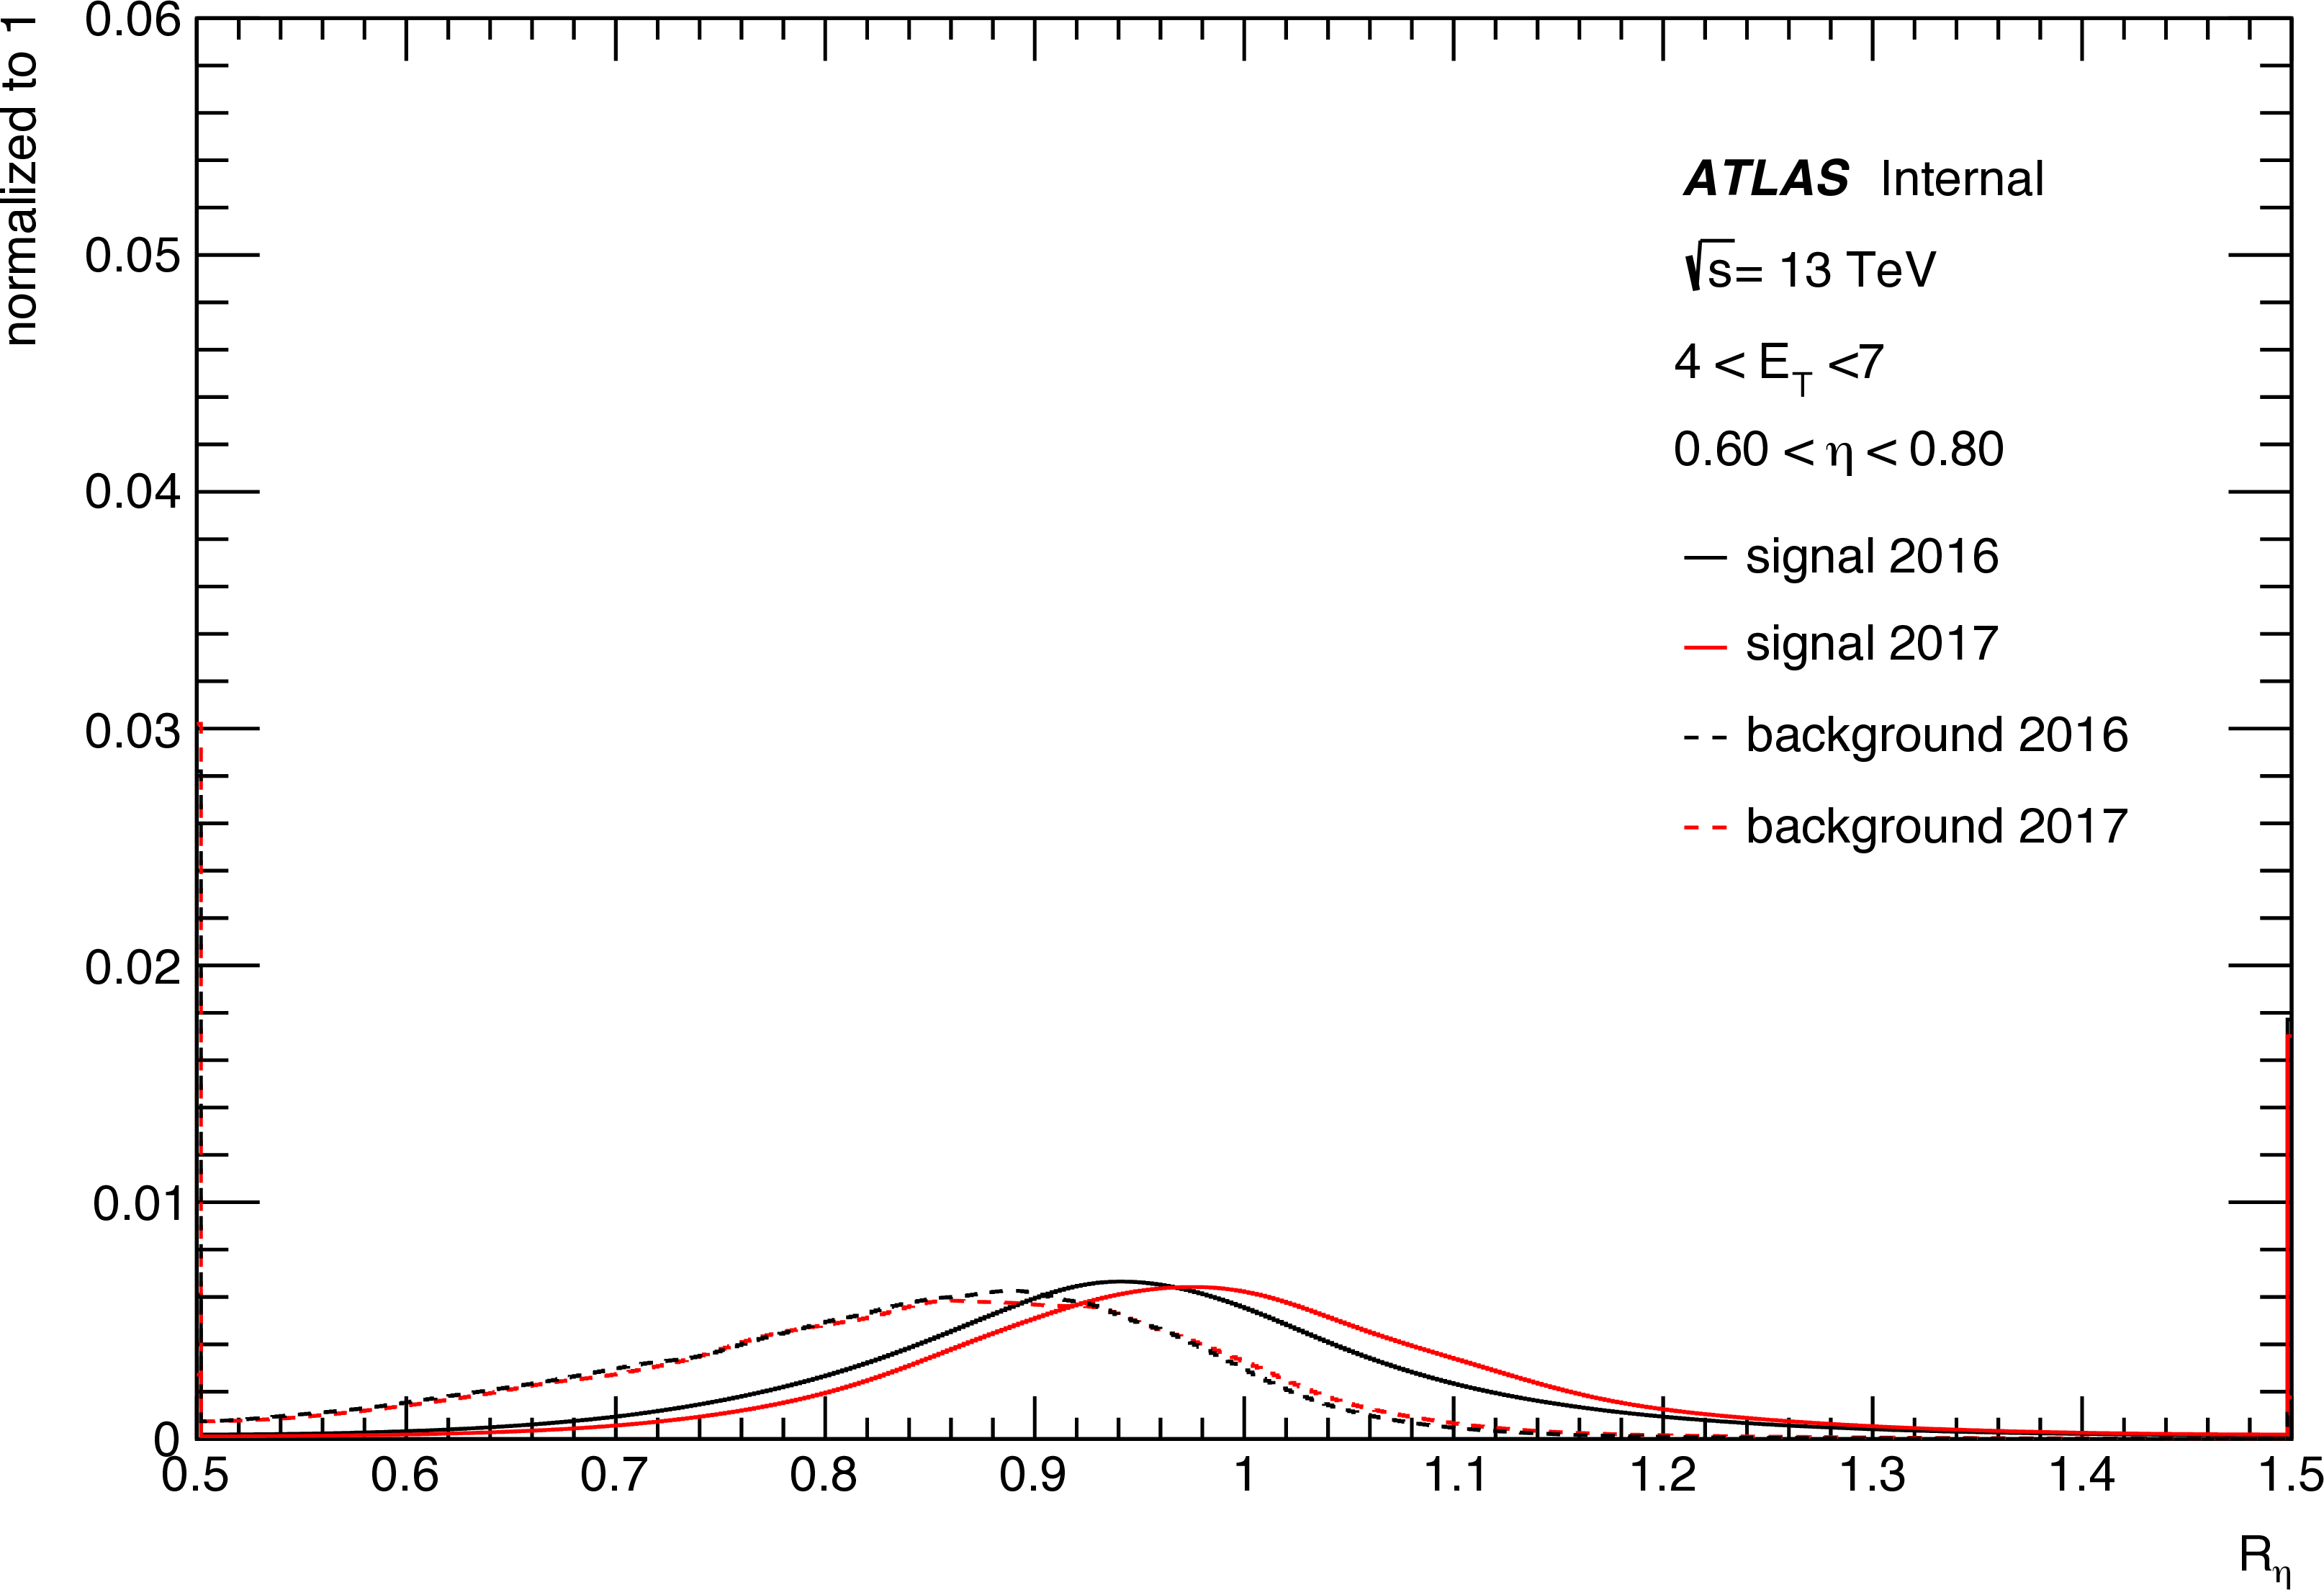
\includegraphics[width=1.0\textwidth]{figs/egamma/trig_reta_lowet.png} 
    \label{fig:egamma:trig_reta_lowet}
  \end{subfigure}
  \caption[Pdfs of tracking and track-cluster matching variables \TRTPID, \deltaeta, \deltaphires, and the shower shape variables \weta, \rhad, and \reta.]{Pdfs of tracking and track-cluster matching variables \TRTPID, \deltaeta, \deltaphires, and the shower shape variables \weta, \rhad, and \reta.
  All of which are defined in Table~\ref{tab:IDcuts} and shown for
  4~\GeV $<$ \et\ $<$ 7~\GeV and $0.6<|\eta|<0.8$.
  The solid line distributions are determined from a background simulation sample and the dashed-line distributions are determined from a \Zee simulation sample.
  The black distributions are pdfs used in the trigger LH in 2016/2017 data taking years and the red are the pdfs developed for the 2018 year.
  These distributions are for reconstructed electron candidates before applying any identification.
  They are smoothed using an adaptive KDE and have been corrected for offsets or differences in widths between the distributions in data and simulation.
  }
\end{figure}
\begin{figure}[t]\ContinuedFloat
\centering
  \begin{subfigure}[b]{0.49\textwidth}
    \centering
    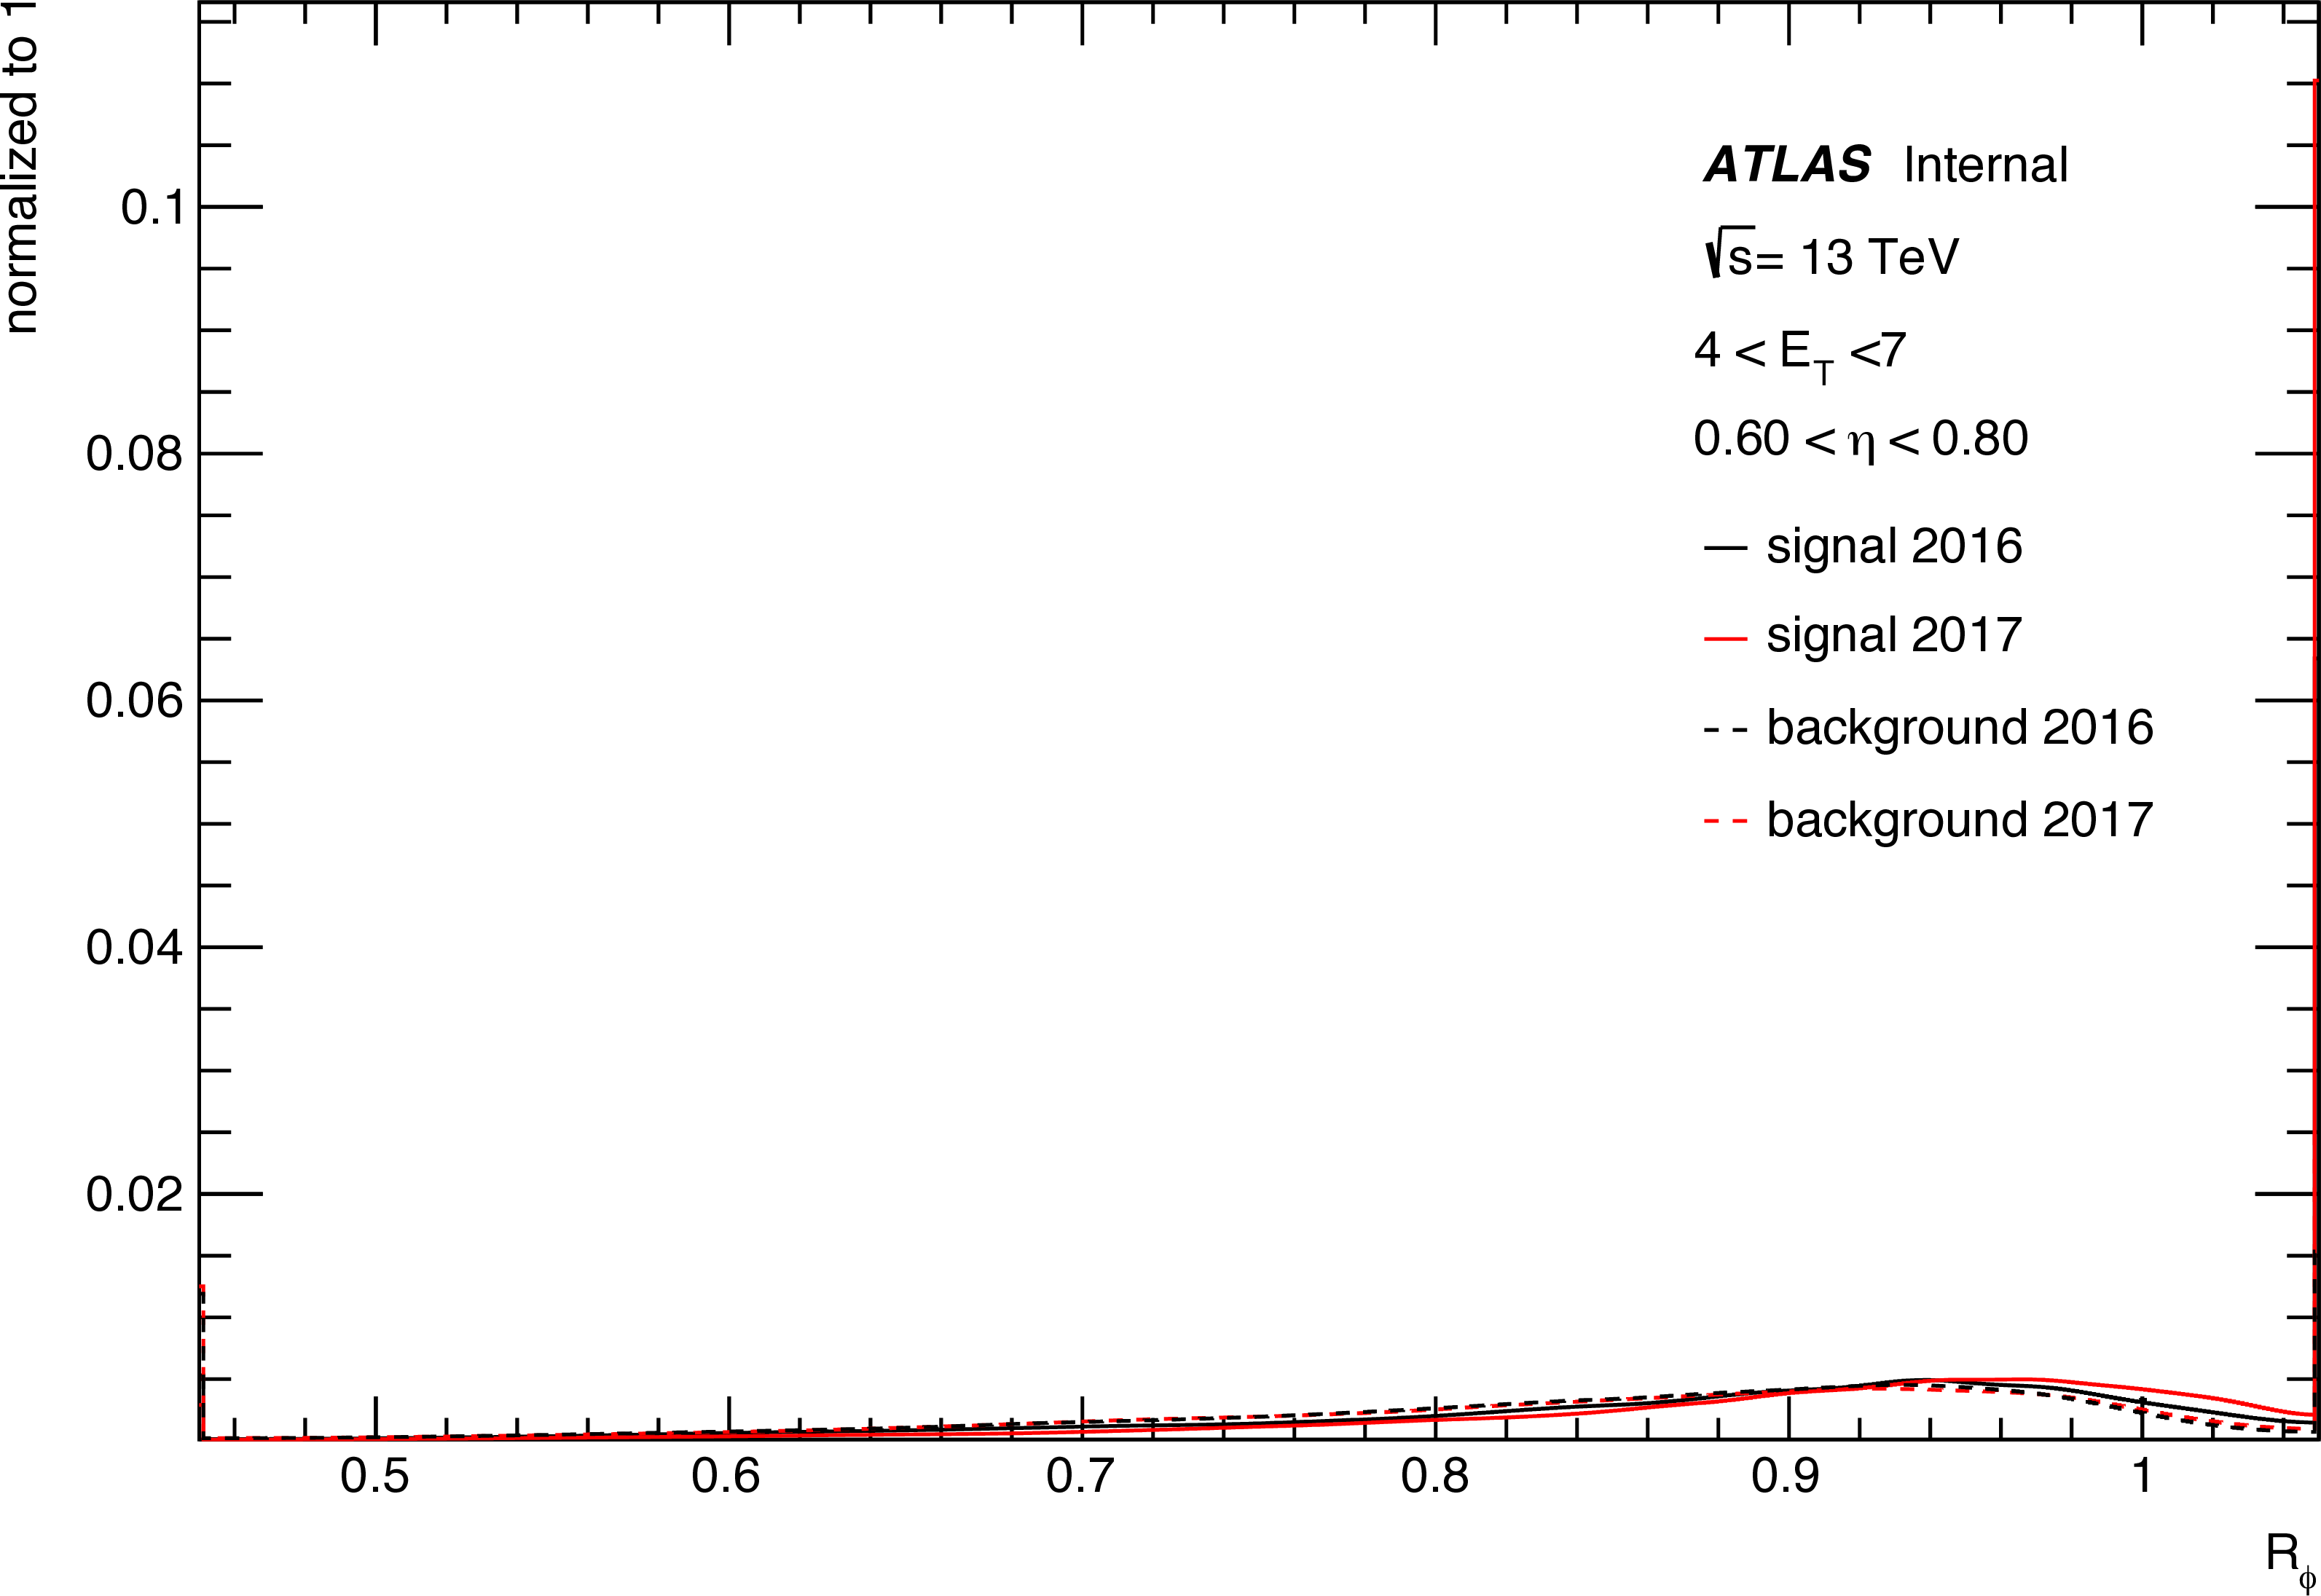
\includegraphics[width=1.0\textwidth]{figs/egamma/trig_rphi_lowet.png} 
    \label{fig:egamma:trig_rph_lowet}
  \end{subfigure}
  \hfill
  \begin{subfigure}[b]{0.49\textwidth}
    \centering
    \includegraphics[width=1.0\textwidth]{figs/egamma/trig_eratio_lowEt.png} 
    \label{fig:egamma:trig_eratio_lowet}
  \end{subfigure}
  \hfill
  \begin{subfigure}[b]{0.49\textwidth}
    \centering
    \includegraphics[width=1.0\textwidth]{figs/egamma/trig_f1_lowet.png} 
    \label{fig:egamma:trig_f1_lowet}
  \end{subfigure}
  \hfill
  \begin{subfigure}[b]{0.49\textwidth}
    \centering
    \includegraphics[width=1.0\textwidth]{figs/egamma/trig_f3_lowet.png} 
    \label{fig:egamma:trig_f3_lowet}
  \end{subfigure}
  \caption[Pdfs of shower shape variables \rphi, $E_{\mathrm{ratio}}$, \fI, and \fIII]{Pdfs of shower shape variables \rphi, $E_{\mathrm{ratio}}$, \fI, and \fIII.
  All of which are defined in Table~\ref{tab:IDcuts} and shown for
  4~\GeV $<$ \et\ $<$ 7~\GeV and $0.6<|\eta|<0.8$.
  The solid line distributions are determined from a background simulation sample and the dashed-line distributions are determined from a \Zee simulation sample.
  The black distributions are pdfs used in the trigger LH in 2016/2017 data taking years and the red are the pdfs developed for the 2018 year.
  These distributions are for reconstructed electron candidates before applying any identification.
  They are smoothed using an adaptive KDE and have been corrected for offsets or differences in widths between the distributions in data and simulation.
}
\label{fig:egamma:trig_pdfs_lowet}
\end{figure}

High \et\ pdfs in Figure~\ref{fig:egamma:trig_pdfs_highet} show very good agreement with the previous pdf set as well as an expected, with the exception of \TRTPID, systematic broadening of signal distributions due to the higher pileup data used to build the pdfs (2017 data vs. 2015-2016 data).
The large differences for \TRTPID\ are due to a re-optimization of the \TRTPID\ (a likelihood itself) for an updated gas configuration.
Low \et\ pdfs in Figure ~\ref{fig:egamma:trig_pdfs_lowet} also show good agreement with several distributions showing narrower signal distributions.
Note that here we are now comparing data pdfs (built of 2017 data) to MC pdfs with simple data-MC shift and width corrections applied and so we do expect differences coming from mis-modeling in MC.
Via the discriminant tuning procedure described in Section~\ref{sec:egamma:tuning} discriminant values are determined using the high-$\mu$ MC sample s.t. desired signal efficiencies are met.
Additionally the $n_{vtx,\text{max}}$ ($\mu_{\text{max}}$ for Trigger LH) value described in Section~\ref{sec:egamma:pileup}, and illustrated in Figure~\ref{fig:egamma:piecewise}, was increased from $\mu_{\text{max}}$ = 50 to $\mu_{\text{max}}$ = 100.

Trigger rates were determined using a trigger emulation tool for four standard electron triggers for the three cases, using the nominal (old) LH \tune, using the new updated LH \tune, and using the new updated LH \tune\ along with the new ``ringer'' fast calorimeter reconstruction algorithm\footnote{
The ringer algorithm is a neural-network based fast-calorimeter reconstruction algorithm that uses all calorimeter layers, centered in a window around the cluster barycenter. 
Each ring is the collection of cells around the previous one.
Ring value is the sum \ET\ of all cells of that ring. Achieves same signal efficiency as cut-based method but with a 50\% reduction in CPU demand for the lowest unprescaled single electron trigger.}.
These rates are shown in Table~\ref{tab:trig_rates}.

\begin{table}[h]
\footnotesize
\renewcommand{\arraystretch}{1.16}
\begin{center}
  \begin{tabular}{|l|l|l|l|}
\hline
\textbf{Trigger} & \textbf{Nominal Rate} & \textbf{Rate w/ new LH} & \textbf{Rate w/ new LH and Ringer} \\
\hline
e26\_lhtight\_nod0\_ivarloose & 201~Hz & 197~Hz & 197~Hz \\
\hline
e28\_lhtight\_nod0\_ivarloose & 175~Hz & 172~Hz & 172~Hz \\
\hline
e60\_lhmedium\_nod0\_L1EM24VHI & 23.5~Hz & 25.3~Hz & 25.3~Hz \\
\hline
2e17\_lhvloose\_nod0\_L12EM24VHI & 12.5~Hz & 12.3~Hz & 12.5~Hz \\
\hline
\end{tabular}
\end{center}
  \caption{Trigger rates determined using a trigger emulation tool for four standard electron triggers for the three cases; using the nominal (old) LH \tune, using the new updated LH \tune, and using the new updated LH \tune\ along with the new ``ringer'' fast calorimeter reconstruction algorithm.}
\label{tab:trig_rates}
\end{table}
Small improvement expected with the new \tune\ for electron
triggers but all changes are within statistical uncertainties.
No increase of rate expected with new \tune.
Efficiencies taken from a full data run reprocessed with Tier 0 monitoring were produced for standard electron triggers that use \Tight, \Medium, and \VeryLoose\ operating points are shown in Figure~\ref{fig:egamma:trig_eff}.
Three cases are compared: new offline LH \tune\ numerator and new online LH \tune\ denominator in black, old offline LH \tune\ numerator and old online LH \tune\ denominator in red, and new offline LH \tune\ numerator and old online LH \tune\ denominator in blue.

\begin{figure}[hp]
\centering
  \begin{subfigure}[b]{1.00\textwidth}
    \centering
    \includegraphics[width=1.0\textwidth]{figs/egamma/trig_eff_lhtight.png} 
    \label{fig:egamma:trig_eff_lhtight}
  \end{subfigure}
  \begin{subfigure}[b]{1.00\textwidth}
    \centering
    \includegraphics[width=1.0\textwidth]{figs/egamma/trig_eff_lhmedium.png} 
    \label{fig:egamma:trig_eff_lhmedium}
  \end{subfigure}
  \begin{subfigure}[b]{1.0\textwidth}
    \centering
    \includegraphics[width=1.0\textwidth]{figs/egamma/trig_eff_lhvloose.png} 
    \label{fig:egamma:trig_eff_lhvloose}
  \end{subfigure}
  \caption{Efficiencies taken from a full data run reprocessed with Tier0 monitoring as a function of $\langle\mu\rangle$ and \et\ produced for standard electron triggers that use the \Tight\ (top), \Medium\ (middle), and \VeryLoose\ (bottom) operating points.
  Three cases are compared: new offline LH \tune\ numerator and new online LH \tune\ denominator in black, old offline LH \tune\ numerator and old online LH \tune\ denominator in red, and new offline LH \tune\ numerator and old online LH \tune\ denominator in blue.}
\label{fig:egamma:trig_eff}
\end{figure}
The new online LH \tune\ performed better than previous \tune\ for all operating points with the exception of the \Medium\ operating point at high $\mu$.
While further investigation on this discrepancy was recommended, due to the short timeline associated with having a validated trigger menu in place before data taking, the decision was made to update all operating points except \Medium, which would retain the previous year's version for the trigger LH (the blue triangle markers).
This new Trigger LH \tune\ was implemented in March 2018.

%Photon and electron reconstruction at the HLT stage is performed on each EM RoI provided by L1, which satisfies \et{} and isolation requirements as specified by the trigger menu.
%It proceeds in a series of sequential steps as shown in Figure~\ref{fig-seq}. 
%In the HLT, fast algorithms are executed first, allowing precision algorithms  (which closely reproduce the offline algorithms and require more CPU time)  to run at a reduced rate later in the trigger sequence. 
%Fast algorithms are executed using calorimeter and ID information within the RoI to perform the initial selection and identification  of the photon and electron candidates, and achieve early background rejection.
%If a particle candidate satisfies the criteria defined for the fast selection, the precision algorithms are executed in the HLT, where access to detector information outside the RoI is possible.

%Another source of inefficiency is the L2 trigger decision. At L2, only a “fast algorithm” version of the cluster is available (in 2012—beginning in 2015 a track from a fast algorithm is available as well).
%The L2 trigger decision must take 100K events from L1 and reduce it to 10K events. Since tracking information is unavailable at L2, rectangular cuts are used to reduce the rate.
%In particular, the cuts mixed with a likelihood at HLT will cause inefficiencies. (These inefficiencies could be reduced in the future by replacing the rectangular cut approach with an MVA, such as a likelihood using only calorimeter variables.)

